%-----Преамбула
\documentclass[a4paper,12pt,oneside,openbib]{book}


%-----Используемые пакеты
%-общие пакеты
\usepackage{indentfirst}
\usepackage[cp1251]{inputenc}
\usepackage[T2A]{fontenc}
\usepackage[english,russian]{babel,varioref}
\usepackage{makeidx}
\usepackage[centerlast,small]{caption2}
\usepackage{textcomp}
%-графика
\usepackage[dvips]{graphicx}
\usepackage{color}
\usepackage{epic,bez123}
\usepackage{floatflt}
%\usepackage{wrapfig}
\usepackage{subfigure}
\usepackage{ifpdf}
\usepackage{pgf}
\usepackage{pstricks}%variant: \usepackage{pst-all}


%-математика
%\usepackage{theorem}
\usepackage[psamsfonts]{amssymb}
\usepackage{amsmath,amsfonts}
\usepackage{amsthm}
\usepackage[mathscr]{eucal}
\usepackage{enumerate}


%-----Стили математических переменных окружения

\newtheoremstyle{break}% name
  {9pt}%      Space above, empty = `usual value'
  {9pt}%      Space below
  {\itshape}% Body font
  {}%         Indent amount (empty = no indent, \parindent = para indent)
  {\bfseries}% Thm head font
  {.}%        Punctuation after thm head
  {\newline}% Space after thm head: \newline = linebreak
  {}%         Thm head spec


\newtheoremstyle{note}% name
  {9pt}%      Space above
  {9pt}%      Space below
  {\itshape}%         Body font
  {}%         Indent amount (empty = no indent, \parindent = para indent)
  {\bfseries}% Thm head font
  {.}%        Punctuation after thm head
  {.5em}%     Space after thm head: " " = normal interword space;
        %       \newline = linebreak
  {}%         Thm head spec (can be left empty, meaning `normal')


\newtheoremstyle{commnt}% name
  {9pt}%      Space above, empty = `usual value'
  {9pt}%      Space below
  {\slshape}  % Body font
  {}%         Indent amount (empty = no indent, \parindent = para indent)
  {\bfseries \slshape}% Thm head font
  {.}%        Punctuation after thm head
  {\newline}% Space after thm head: \newline = linebreak
  {}%         Thm head spec

%-----Математические переменные окружения
\theoremstyle{break}
\newtheorem{teo}{Теорема}[chapter]
\newtheorem{lem}[teo]{Лемма}
\newtheorem{sta}[teo]{Утверждение}
\newtheorem{prop}[teo]{Предложение}
\newtheorem{dfn}{Определение}[chapter]

\theoremstyle{plain}
\newtheorem{axi}{Предположение}[section]
\newtheorem*{corol}{Следствие}
\newtheorem{teop}[teo]{Теорема}
\newtheorem{lemp}[teo]{Лемма}

\theoremstyle{definition}
\newtheorem{exer}{Упражнение}[chapter]
\newtheorem*{note}{Замечание}

\theoremstyle{commnt}
\newtheorem*{comm}{Экономический комментарий}
\newtheorem*{exam}{Пример}

%-----Инициализация команд
\newcommand{\conts}{\usefont{T2A}{cmr}{m}{ui}}
\newcommand{\remrk}[1]{\bigskip\texttt{#1}\bigskip}
\newcommand{\R}{\mathbb{R}}
\newcommand{\Lgr}{\mathscr{L}}
\newcommand{\st}[1]{\mathbb{#1}}
\newcommand{\vc}[1]{\mathbf{#1}}
\newcommand{\dw}[1]{\textsl{\textbf{#1}}}

%-----Переинициализация команд
\renewcommand{\chaptername}{Модуль}
\renewcommand{\captionlabeldelim}{.}
%\renewcommand{\bibname}{Список основной литературы \\к книге\\<<Введение в математическую экономику>>}
%\renewcommand{\baselinestretch}{1.25}
\makeatletter
\renewcommand{\@seccntformat}[1]{\csname the#1\endcsname.\hspace{1em}}
\makeatother


%-----Настройки
%\makeindex

%\setlength{\intextsep}{50pt}

%\setlength{\abovecaptionskip}{-5pt}

\sloppy

\graphicspath{{pics/}}
\includeonly{predvelich, 02_Linear, convex, nelin-opt, Raznoe}

\title{Материалы для книги \\ <<Введение в математическую экономику>>}
\author{}
\date{\today}


%====================================НАЧАЛО ДОКУМЕНТА
\begin{document}
\maketitle


%-----Предисловие
\frontmatter
\chapter{�������� �����������}

\section*{�������}
����������� ��� ��������:

$i=1 \ldots m$ --- ������, ����������� �������� �� 1 �� $m$; �������� ���������� �������
\remrk{??????} ������;

$j=1 \ldots n$ --- ������, ����������� �������� �� 1 �� $n$; �������� ���������� ������
\remrk{??????} ������;

$k=1 \ldots q$ --- ������, ����������� �������� �� 1 �� $q$;

$l=1 \ldots r$ --- ������, ����������� �������� �� 1 �� $r$.

\section*{���������, �������, �����}

��������� � ������������ �������� ������������ \texttt{����������}
���������� ���������� �������, ��������, $\st{X}$ ��� $\st{Y}$.

    ����� $\mid$ � $:$ ������������ ��� �������� �������� ������ �������������� <<����� ���>>.
    ��������, ������
\[
    \{\vc{x}\in \st{X} \mid \vc{x}\in \st{Y}\},
\]
    ��� � ������
\[
    \{\vc{x}\in \st{X} : \vc{x}\in \st{Y}\},
\]
    ����� �������������� ��� ����������� ����������� $\st{X}\cap\st{Y}$ �������� $\st{X}$ �
    $\st{Y}$, � ������
\[
    \{x\in\R^{1} \mid \exists z\in\R^{1} : x=z^{2}+1\}
\]
    --- ��� ��������� ���������� �����������  ��������� $[1,+\infty)$.

�������� $\R^n$ ������������ $n$-������ ��������� ������������, ���������� �������� ��������
$n$-������������ ������� (������� ��� ������).

��� ����������� �������� ������������ ������������
\texttt{���������} �����. �������-������� ������������ $\R^n$
������������ ����������� ��������� �������, � �� ���������� ---
��������� ������� � ������� ���������:

\[
\vc{x} = \left( {\begin{array}{*{20}c}
   {x_1 }  \\
   {x_2 }  \\
    \vdots   \\
   {x_n }  \\
\end{array}} \right) \in \R^n
\]

\noindent �������-������ ����� ������������ ����������� ���������
������� (������� ����� ���������-��������� � ���������-��������
����� ���� �� ��������� ��� �������� ����������������):

\[
\vc{p} = (p_1 ,p_2 , \ldots ,p_n ) \in \R^n
\]

� ������� �� ��������, ��� ����������� ������� (������������) �����
������������ \texttt{���������} �����, ��������, $\alpha$, $\beta$,
$\gamma$, $\theta$, $\pi$. ��������������, ��� ��� ��� ����� �
��������� $\R$.


\section*{�������� ��� ���������}

����� $\vc{x},\vc{y} \in \st{X} \subset \R^n$. ����� ����������:

\begin{itemize}
  \item $\vc{y} \geqq \vc{x}$, ���� $y_i \geq x_i$, $i=1 \ldots n$;
  \item $\vc{y} \geq \vc{x}$, ���� $y_i \geq x_i$, $i=1 \ldots n$, � ���� �� ���� ��
���������� ��\-��������� ��� �������;
  \item $\vc{y} \gg \vc{x}$, ���� $y_i > x_i$, $i=1 \ldots n$.
\end{itemize}

����� $\vc{p}$ --- ������-������ �� $\R^n$, � $\vc{x}$ ---
������-������� �� $\R^n$. �����

\[
\vc{p} \cdot \vc{x} = p_1 x_1 + p_2 x_2 + \ldots + p_n x_n = \sum
\limits_{i=1}^n p_i x_i,
\]

\noindent ��� ����� ���������� ��� ������������ ������ �� �������
��� \emph{��������� ������������}\index{��������� ������������}.


\section*{�������}

������� ������������ ���������� ���������� �������.

$A$ --- ������� ������������� ��������������� ������; �����������
������� ����������� ������ ��������, ��������, $A_{m\times n}$.

������� ������� $A_{m\times n}$ (�������-�������) ������������
$\vc{a}^1, \vc{a}^2, \ldots, \vc{a}^n$. ������ ������� $A_{m\times
n}$ (�������-������) ������������ $\vc{a}_1, \vc{a}_2, \ldots,
\vc{a}_m$. ������� � ������ ����� ���������� ���������� �������.
��������� �������� ������� ������������ $a_{ij}$, ��� $i=1 \ldots
n$, $j=1 \ldots m$. (� ���� ��� ��������. ��� ���������???????)

����� �������, ������� $A$ ����� ���� ������������ ��� �����
��������-�����, ��������-�������� ��� ��������� ���������, ���
�������� ����:

\[
A = \left( {\begin{array}{*{20}c}
   {\vc{a}_1 }  \\
   {\vc{a}_2 }  \\
    \vdots   \\
   {\vc{a}_m }  \\
\end{array}} \right) = \left( {\vc{a}^1 ,\vc{a}^2 , \ldots ,\vc{a}^n } \right) = \left( {\begin{array}{*{20}c}
   {a_{11} } & {a_{12} } & {a_{13} } &  \ldots  & {a_{1n} }  \\
   {a_{21} } & {a_{22} } & {a_{23} } &  \ldots  & {a_{2n} }  \\
    \ldots  &  \ldots  &  \ldots  &  \ldots  &  \ldots   \\
   {a_{m1} } & {a_{m2} } & {a_{m3} } &  \ldots  & {a_{mn} }  \\
\end{array}} \right)
\]


��� ���������� ������� ����������� ������������ ����� ������,
��������, $B_{n}$.

��������� ������� ������������ ��� $E$.



%-----Основная часть
\mainmatter




\chapter{Предельные величины в экономике}

\section{ Максимумы и минимумы. Производные. Выпуклые и вогнутые функции}


\subsection{Простейшие задачи на максимум и минимум}


    Ключевая роль предельных величин в экономической науке определяется тем,
    что важнейшее предположение о поведении экономических агентов при построении
    тех или иных моделей  состоит в том, что ведут они себя рационально,  т.е.
    решают задачи на максимум или минимум. Понятия максимума и минимума
    объединены терминами <<оптимум>> и <<экстремум>>. Задачи на отыскание максимума
    и минимума называют оптимизационными или экстремальными
    задачами, а раздел математики, в котором
    изучают такие задачи, называется теорией оптимизации или теорией
    экстремальных задач.
    А анализ таких задач удобнее всего
    проводить именно на языке предельных величин, т.е. с помощью
    дифференциального исчисления. В этом пункте мы напомним
    читателю, как проводить этот анализ в самых простейших ситуациях.



    Напомним читателю основные определения.

    Пусть $\st{D}$ --- некоторое подмножество вещественной прямой
    $\R$, а функция $f$ определена на
    всей вещественной прямой или на некотором ее подмножестве,
    содержащем $\st{D}$ (быть может, только на самом $\st{D}$).
    Точка $x^{*}\in \st{D}$ называется точкой \emph{глобального
    максимума}, или просто точкой максимума, функции
     $f$ (на множестве $\st{D}$), если
    \[f(x^{*})\geqslant f(x) \ \forall x\in\st{D},\]
    и точкой \emph{глобального минимума}, или просто точкой минимума, если
     \[f(x^{*})\leqslant f(x) \ \forall x\in\st{D}.\]
     Если же существует  окрестность
     \[(\hat{x}-\epsilon,x^{*}-\epsilon), \  \epsilon>0,\]
     точки $x^{*}$, такая что
     \[f(x^{*})\geqslant f(x) \ \forall x\in\st{D}\cap(x^{*}-\epsilon,x^{*}-\epsilon)\]
     или
     \[f(x^{*})\leqslant f(x) \ \forall x\in\st{D}\cap(x^{*}-\epsilon,x^{*}-\epsilon),\]
     то эта точка называется точкой локального максимума или локального
     минимума соответственно.


     Точки (локального) максимума и минимума называются точками (локального) экстремума.
     Очевидно, что всякая точка максимума (минимума) является точкой
     локального максимума (минимума), но не наоборот.

     Задачу об отыскании максимума функции $f$ на множестве $\st{D}$
     записывают в виде
\begin{equation*}
\label{z-max-odnom}
     f(x)\rightarrow \max, \ x\in\st{D},
\end{equation*}
          а задачу об отыскании минимума --- в виде
\begin{equation}
\label{z-min-odnom}
     f(x)\rightarrow \min, \ x\in\st{D}.
\end{equation}


     При это зачастую не уточняют, идет ли речь о локальном или же
    о глобальном экстремуме. Из
     контекста всегда понятно, о чем идет речь. В экономических
     задачах обычно речь идет именно о глобальном экстремуме. Нас тоже будет
    интересовать глобальный максимум или минимум.
    Поэтому под
     решением задачи на максимум мы всегда будем понимать точку
     глобального максимума, а под решением задачи на минимум ---
     точку глобального минимума.

      Функция $f$,
     экстремум которой ищется, называется \emph{целевой функцией}, а
     множество $\st{D}$, на котором нужно найти этот экстремум,
     называют \emph{допустимым множеством}. Значение целевой функции в точке
    экстремума называется (оптимальным) \emph{значением задачи}.

     Первый вопрос, который заслуживает обсуждения после того, как
     сформулирована задача на экстремум, это вопрос о
     том, существует ли искомая точка максимума или минимума. Ответ
     на него зависит от устройства целевой функции и допустимого
     множества. Про целевую функцию почти всегда предполагают, что
     она непрерывна. Что касается допустимого множества, то чаще
     всего в содержательных задачах это множество является всей
     вещественной прямой $\R$ или замкнутым промежутком (например,
     отрезком $[\bar{x},\bar{\bar{x}}]$ или замкнутой полупрямой
     $[\bar{x},+\infty)$,
     первым примером которой является множество $\R_{+}$ всех
     неотрицательных чисел).

    На отрезке, представляющем собой компактное множество,
    непрерывная функция достигает своего максимума и минимума. Об
    этом говорит известная теорема Вейерштрасса (??????).

    Если же допустимое
    множество является хотя и замкнутым, но неограниченным, например всей вещественной
    прямой или полупрямой, то максимум или минимум непрерывной
    функции на этом множестве может и не достигаться. Например, на
    множестве $\R_{+}$ функция $f(x)=x^{1/2}$ достигает своего
    минимума (в нуле), но не достигает максимума, а функция
    $f(x)=x^{1/2}-x$ достигает своего максимума в некоторой положительной
    точке, но не достигает своего минимума.







\


    Как мы уже говорили, исследовать задачи на экстремум удобно с
    помощью дифференциального исчисления.
    Напомним, что функция $y=f(x)$, заданная в некоторой окрестности
    точки $\hat{x}\in\R$,  называется дифференцируемой в этой точке,
    если существует такая линейная функция $a\Delta x$
    (ее аргументом является $\Delta x$), что приращение
    \[\Delta y=f(x+\Delta x)-f(x)\]
    функции $f$ представимо в виде
\begin{equation}
\label{differents}
    \Delta y=a\Delta x+o(\Delta x) \ \text{при} \ \Delta x\rightarrow 0,
\end{equation}
    где, как обычно, символ $o(\cdot)$ используется для обозначения
    бесконечно малой.
    Иными словами, функция дифференцируема в точке $\hat{x}\in\R$,
    если изменение ее значения в окрестности исследуемой точки
    линейно с точностью до поправки, бесконечно малой по сравнению с
    величиной смещения от $\hat{x}\in\R$. Линейная функция $a\Delta x$,
    фигурирующая в (\ref{differents}), называется дифференциалом
    функции $f$ в точке $\hat{x}\in\R$ (ее аргументом является $\Delta x$).
    Читатель, несомненно помнит, что  дифференцируемость функции $f$ в
    точке $\hat{x}\in\R$ эквивалентна существованию конечной производной
    $f\,'(\hat{x})$, при этом последняя совпадает с числом $a$,
    задающим линейную функцию $a\Delta x$.

    Далее в этой главе мы иногда будем записывать соотношение (\ref{differents}) в
    виде
    \[\Delta y\approx a\Delta x=f\,'(\hat{x})\Delta x,\]
    а слова о том, что некоторое равенство выполняется с точностью
    до бесконечно малой, заменять словами о том, что равенство
    является примерным или приближенным. (\remrk{РИС ???????})
    При этом, мы зачастую будем
    проводить рассуждения, считая что что приращение  $\Delta x$
    задано, но что оно достаточно мало, а точность примерного
    равенства достаточно высока. Наши рассуждения будут
    не самыми строгими, но если читатель достаточно хорошо знаком с
    математическим анализом, он сможет перевести их на
    самый точный математический язык.

    В дальнейшем само по себе использование обозначения $f\,'(x)$
    будет автоматически подразумевать, что функция $f(x)$ дифференцируема в точке
    $x$, на всей области своего определения
    или на внутренности этой области. Соответственно,
    использование обозначения $f\,''(x)$ будет свидетельствовать о
    том, что речь идет о дважды дифференцируемой функции.

    Кроме
    того, мы будем допускать некоторую вольность и называть функцию
    дифференцируемой, если у нее имеется производная, быть может,
    даже бесконечная и, быть может, односторонняя. Например, функцию
    $f(x)=x^{1/2}$ мы будем считать дифференцируемой. Для нее
    $f'(0)=+\infty$.

    Теперь напомним, как производные применяются для анализа задач
    на экстремум.
    Далее в этом параграфе, если не оговорено противное, мы будем
    вести речь о задачах на максимум. С качественной точки зрения
    анализ задач на минимум ничем не отличается от задач на
    максимум, поскольку задачу на минимум
    (\ref{z-min-odnom}) можно переписать в виде
    \[-f(x)\rightarrow \max, \ x\in\st{X}.\]

    Рассмотрим следующую совсем простую задачу:
\begin{equation}
\label{monot-max}
    f(x)\rightarrow \max, \ x\in[\bar{x},\bar{\bar{x}}\,], \ -\infty<\bar{x}<\bar{\bar{x}}<+\infty,
\end{equation}
    где $f(x)=b+ax$.
    Очевидно, что ее решение зависит от того, чему равно $a$. Если
    $a>0$, то решением (точкой глобального максимума) является точка
    $\bar{\bar{x}}$, если $a<0$, то точка $\bar{x}$, а если $a=0$, то решением
    рассматриваемой задачи является любая точка отрезка $[\bar{x},\bar{\bar{x}}\,]$.
    Здесь ключевую роль играет то, что в случае $a>0$ функция $f$
    монотонно возрастает на всем отрезке $[\bar{x},\bar{\bar{x}}\,]$, а при $a<0$ она
    монотонно убывает. Для нас важно то, что в случае монотонно возрастающей
    функции никакая внутренняя точка отрезка не является точкой
    локального максимума.
    (\remrk{РИС ???????, a>0, a<0, a=0})

      Это простое рассуждение позволяет понять, почему при решении
    задачи на экстремум первое, что рекомендуется сделать, это взять
    производную и приравнять ее к нулю (хотя иногда эта
    рекомендация может оказаться неполной или даже неуместной).

    Напомним, что если $f\,'(\hat{x})>0$,
    то функция $f$ \emph{монотонно возрастает} в точке $\hat{x}$, т.е. при
    некотором достаточно малом $\epsilon>0$ выполняются неравенства
    \[f(x)<f(\hat{x}) \ \forall x\in(\hat{x}-\epsilon,\hat{x})\]
    и
    \[f(\hat{x})<f(x) \ \forall x\in(\hat{x},\hat{x}+\epsilon),\]
    поскольку при $b=f(\hat{x}), \ b=f\,'(\hat{x})>0$ и
    $x\in(\hat{x}-\epsilon,\hat{x}+\epsilon)$
    примерное  равенство
    \[f(x)\approx b+ax\]
    является достаточно точным (благодаря тому, что $\epsilon>0$ достаточно мало),
    а функция $b+ax$ монотонно возрастает.


    Если же $f\,'(\hat{x})<0$, то функция $f$ \emph{монотонно убывает}
    в точке $\hat{x}$, т.е. при
    некотором достаточно малом $\epsilon>0$ выполняются неравенства
    \[f(x)>f(\hat{x}) \ \forall x\in(\hat{x}-\epsilon,\hat{x})\]
    и
    \[f(\hat{x})>f(x) \ \forall x\in(\hat{x},\hat{x}+\epsilon).\]


     Заметим, что если $f\,'(\hat{x})=0$, то
    возможна как ситуация, когда функция $f$ не является монотонной
    в точке $\hat{x}$ (например, если $f(x)=x^{2}, \ \hat{x}=0$), так и ситуация,
    когда она монотонно возрастает ($f(x)=x^{3}, \ \hat{x}=0$) или
    убывает ($f(x)=-x^{3}, \ \hat{x}=0$).

    В случае, когда $f\,'(x)>0$ ($f\,'(x)<0$) для всех точек $x$ из
    некоторого интервала вещественной прямой, то функция $f$ возрастает
    (убывает) на всем интервале. (\remrk{Нужен ли этот абзац???????})
    (\remrk{РИС ??????? f'><=0})

    Читатель, несомненно знаком со следующей теоремой.


\begin{teo}
    Предположим, что функция $f$, заданная на некотором промежутке
    $\langle \bar{x},\bar{\bar{x}}\rangle$, дифференцируема в точке
    $\hat{x}\in(\bar{x},\bar{\bar{x}})$.
    Если $\hat{x}$ является точкой локального
    максимума (на $\R$), то
    \[f\,'(\hat{x})=0.\]
\end{teo}
    \textbf{Доказательство.} Достаточно заметить. что если $f'(\hat{x})>0$,
    то функция $f$ монотонно возрастает в точке $\hat{x}$,  а если
    $f\,'(\hat{x})<0$, то монотонно убывает. \ $\Box$


    Из этой теоремы следует, что в случае, когда множество $\st{D}$
    открыто, например, совпадает со всей вещественной прямой $\R$,
    а функция $f$ задана на этом множестве и
    дифференцируема на нем, то решение задачи (\ref{z-min-odnom})
    следует искать среди тех точек $x\in\st{D}$, для которых
    $f\,'(x)=0$. (\remrk{РИС ???????}) Такие точки называют \emph{подозрительными на
    экстремум}. При этом следует подчеркнуть, что среди этих точек
    находятся как все точки локального
    максимума, так и все точки локального минимума, а также точки,
    не являющиеся ни теми, не другими. Иными словами, равенство
    производной нулю не является достаточным условием максимума или
    минимума.

    Напомним, что необходимые и достаточные условия --- это не одно и то же.
    Например, равенство производной нулю в
    сформулированной только что теореме, является необходимым
    условием локального экстремума. Если некоторая точка из
    интервала  $\langle \bar{x},\bar{\bar{x}}\rangle$
    является точкой локального максимума или минимума, то она
    удовлетворяет этому условию. Когда речь идет о достаточном
    условии максимума или минимума, то это значит, что если некоторая точка
    удовлетворяет этому условию, то она обязательно является
    точкой максимума или минимума соответственно.

    Следует указать, что необходимые и/или достаточные условия
    экстремума, формулируемые в терминах первых производных,
    называют \emph{условиями первого порядка}.

    В случае, когда допустимое множество $\st{D}$ является отрезком
    $[\bar{x},\bar{\bar{x}}]$, замкнутой полупрямой (вида $[\bar{x},+\infty)$ или
    $(-\infty,\bar{\bar{x}}]$), точками, \emph{подозрительными на экстремум} являются
    также граничные точки $\st{D}$. А именно, если локальный
    максимум (минимум)
    функции $f$ на отрезке $[\bar{x},\bar{\bar{x}}]$ или
    полупрямой $[\bar{x},+\infty)$ достигается
    в точке $\bar{x}$, то $f\,'(\bar{x})\leqslant0$
    ($f\,'(\bar{x})\geqslant0$). Если же локальный
    максимум (минимум)
    функции $f$ на отрезке $[\bar{x},\bar{\bar{x}}]$ или
    полупрямой $(-\infty,\bar{\bar{x}}]$)
    достигается в точке $\bar{\bar{x}}$, то
    $f\,'(\bar{\bar{x}})\geqslant0$ ($f\,'(\bar{\bar{x}})\leqslant0$).
    (\remrk{РИС ???????})

    Более того, по  знаку производной на границе допустимого
    множества иногда можно с уверенностью сказать, являются ли они
    точкам локального максимума или минимума. А именно можно
    сформулировать достаточные условия максимума и минимума.


    Например, если $f\,'(\bar{x})<0$ ($f\,'(\bar{x})>0$), то
    точка $\bar{x}$ является точкой локального максимума (минимума) функции $f$ на
    отрезке $[\bar{x},\bar{\bar{x}}]$ или полупрямой $[\bar{x},+\infty)$.
    Если же $f\,'(\bar{\bar{x}})>0$ ($f\,'(\bar{\bar{x}})<0$), то
    точка $\bar{\bar{x}}$ является точкой локального максимума (минимума) функции $f$ на
    отрезке $[\bar{x},\bar{\bar{x}}]$ или полупрямой $(-\infty,\bar{\bar{x}}]$.
    (\remrk{РИС ???????})

    Здесь надо уточнить, что под производной на границе
    отрезка или полупрямой, например в точке $\bar{x}$,
    мы понимаем одностороннюю производную.
    В случае же, когда функция $f$ задана не только на самом отрезке
    $[\bar{x},\bar{\bar{x}}]$ или на полупрямой $[\bar{x},+\infty)$,
    но и в некоторой окрестности точки $\bar{x}$ и
    дифференцируема в этой точке, то читателю можно и не вспоминать, что такое
    односторонняя производная.


\subsection{Выпуклые и вогнутые функции}

    Выпуклые и вогнутые функции играют очень важную роль в
    экономическом анализе. Для случая функций нескольких переменных мы обсудим
    их свойства позднее, а здесь вкратце напомним, каковы основные свойства
    выпуклых и вогнутых функций одной переменной, предполагая, что
    эти свойства читателю уже знакомы из курса математического
    анализа.

    Пусть функция $f$ задана на некотором промежутке
    $\langle \bar{x},\bar{\bar{x}} \rangle$, где $\bar{x}$ может быть равным $-\infty$, а
    $\bar{\bar{x}}$ может быть равным $+\infty$.


    Эта функция называется \emph{выпуклой} (\remrk{РИС ???????}) (на промежутке
    $\langle \bar{x},\bar{\bar{x}} \rangle$), если для любых точек
    $x,y\in\langle \bar{x},\bar{\bar{x}} \rangle$ и любом числе
    $\alpha\in[0,1]$ имеет место неравенство
\begin{equation}
    \label{vipuk}
    f(\alpha x +(1-\alpha)y)\leqslant \alpha f(x)+(1-\alpha)f(y).
\end{equation}
    Если при $x\neq y$ и $\alpha\in(0,1)$ это неравенство является
    строгим, то функция $f$ \emph{строго выпуклой}.
    (\remrk{РИС ???????})

    Если же для любых точек
    $x,y\in\langle \bar{x},\bar{\bar{x}} \rangle$ и любом числе
    $\alpha\in[0,1]$ имеет место неравенство
\begin{equation}
    \label{vipuk}
    f(\alpha x +(1-\alpha)y)\geqslant\alpha f(x)+(1-\alpha)f(y),
\end{equation}
    то функция $f$ называется \emph{вогнутой}. Если при $x\neq y$ и
    $\alpha\in(0,1)$ последнее неравенство является
    строгим, то функция $f$ \emph{строго вогнутой}.
    (\remrk{РИС ???????})

    Иногда выпуклые функции называют выпуклыми вниз, а вогнутые ---
    выпуклыми вверх.

    Очевидно, что если функция $f(x)$ выпукла, то функция $-f(x)$
    вогнута. Отсюда следует, что функция $f(x)=b+ax$ является выпуклой
    и вогнутой одновременно. Конечно, эта функция не является строго выпуклой или строго
    выпуклой.
\begin{exer}
    Предположим, что функции $f(x)$ и $g(x)$ выпуклы.

    Докажите, что функция
    $h(x)=\max\{f(x),g(x)\}$ тоже выпукла. Может ли быть выпуклой
    функция $h(x)=\min\{f(x),g(x)\}$?

    Докажите, что если
    $\alpha\geqslant0$ и $\beta\geqslant0$, то функция $h(x)=\alpha f(x)+\beta g(x)$
    выпукла, а если $\alpha\leqslant0$ и $\beta\leqslant0$, то вогнута.
\end{exer}

\begin{exer}
    Докажите, что если функция выпукла, но не строго выпукла, то ее
    график содержит некоторый отрезок.
\end{exer}

\begin{exer}
    Докажите, что функция $f$ выпукла на промежутке
    $\langle \bar{x},\bar{\bar{x}}\rangle$
    тогда и только тогда, когда для каждого
    $t\in\langle \bar{x},\bar{\bar{x}}\rangle$ функция
    \[g_{t}(x)=\frac{f(x)-f(t)}{x-t},\]
    заданная на промежутке $\langle \bar{x},\bar{\bar{x}}\rangle$ за исключением точки
    $t$, монотонно не убывает.
\end{exer}


    Напомним, как характеризуются выпуклые и
    вогнутые функции в случае, когда они дифференцируемы и дважды дифференцируемы.
\begin{prop}
    Предположим, что функция $f$ непрерывна на промежутке
    $\langle \bar{x},\bar{\bar{x}} \rangle$
     и дифференцируема на внутренности этого промежутка, т.е. на
     интервале $(\bar{x},\bar{\bar{x}})$.

    Эта функция вогнута (выпукла) на $\langle \bar{x},\bar{\bar{x}} \rangle$
    тогда и только тогда, когда
    функция $f\,'$ монотонно не возрастает (не убывает) на $(\bar{x},\bar{\bar{x}})$.
    Функция $f$ строго вогнута (выпукла) на
    $\langle \bar{x},\bar{\bar{x}} \rangle$ тогда и только тогда, когда
     $f\,'$ монотонно убывает (возрастает) на $(\bar{x},\bar{\bar{x}})$.
\end{prop}                          (\remrk{здесь все правильно??????})

\begin{prop}
    \label{kasatel}
    Предположим, что функция $f$ дифференцируема на интервале
    $(\bar{x},\bar{\bar{x}})$.


    Эта функция выпукла (вогнута) на $(\bar{x},\bar{\bar{x}})$ тогда и
    только тогда, когда для любых точек $x,y\in(\bar{x},\bar{\bar{x}})$
    выполняется неравенство
    \[f(y)-f(x)\geqslant f\,'(x)(y-x)\]
    \[(f(y)-f(x)\leqslant f\,'(x)(y-x))\]
    и строго выпукла (строго вогнута) тогда и только тогда, когда
    для любых несовпадающих точек $x,y\in(\bar{x},\bar{\bar{x}})$
    выполняется неравенство
    \[f(y)-f(x)> f\,'(x)(y-x)\]
    \[(f(y)-f(x)< f\,'(x)(y-x)).\]
\end{prop}
    Геометрически это предложение говорит, что выпуклость
    (вогнутость) дифференцируемой на всем интервале
    $(\bar{x},\bar{\bar{x}})$ функции эквивалентна тому, что ее
    график лежит не ниже (выше) любой проведенной к нему касательной. При
    этом для строгой выпуклости (строгой вогнутости) функции
    необходимо и достаточно чтобы все точки графика, за исключением
    самой точки касания, лежали строго выше (строго ниже) этой
    касательной. (\remrk{РИС ???????})


\begin{prop}
    Предположим, что функция $f$ непрерывна на промежутке
    $\langle \bar{x},\bar{\bar{x}} \rangle$
     и дважды дифференцируема на внутренности этого промежутка, т.е. на
     интервале $(\bar{x},\bar{\bar{x}})$.

    Функция $f$ вогнута (выпукла) на
    $\langle \bar{x},\bar{\bar{x}} \rangle$ тогда и только тогда, когда
    \[f\,''(x)\leqslant0 \ \forall x\in(\bar{x},\bar{\bar{x}})\]
    \[(f\,''(x)\geqslant0 \ \forall x\in(\bar{x},\bar{\bar{x}})).\]
    Если
    \[f\,''(x)<0 \ \forall x\in(\bar{x},\bar{\bar{x}})\]
    \[(f\,''(x)>0 \ \forall x\in(\bar{x},\bar{\bar{x}})),\]
    то рассматриваемая функция строго вогнута (строго выпукла).
\end{prop}
    (\remrk{РИС ???????}) (\remrk{РИС ???????}) (\remrk{РИС ???????})

\begin{exer}
    Приведите пример строго выпуклой на $\R$ функции, вторая производная
    которой в некоторой точке обращается в ноль.
\end{exer}

\begin{exer}
    Проверьте следующие функции на (строгую) выпуклость и (строгую)
    вогнутость на множествах их определения при различных возможных
    значениях параметра $\alpha$:
    \begin{itemize}
      \item $f(x)=x^{\alpha}$;
      \item $f(x)=\alpha^{x}$;
      \item $f(x)=\log_{\alpha}x$.
    \end{itemize}
\end{exer}

\begin{exer}
    Докажите следующие соотношения:
    \begin{itemize}
      \item $e^{x}\geqslant1+x \ \forall x\in\R$, причем $e^{x}>1+x \  \forall   x\neq0$;
      \item $\ln x \leqslant x-1  \ \forall x\in\R$, причем $\ln x < x-1 \ \forall  x\neq1$.
    \end{itemize}

\end{exer}




    Перейдем к анализу задач на максимум и минимум для выпуклых и
    вогнутых функций.
    В следующем упражнении читателю предлагается доказать очень
    важное для экономической науки свойство выпуклых и вогнутых функций.


\begin{exer}
    Пусть $f$ представляет собой выпуклую (вогнутую) на интервале
    $\langle \bar{x},\bar{\bar{x}} \rangle$ функцию. Докажите, что любой локальный
    минимум (локальный максимум) функции $f$ на
    $\langle \bar{x},\bar{\bar{x}} \rangle$
    является глобальным минимумом (глобальным максимумом).
\end{exer}

    Другим важным свойством выпуклых и вогнутых функций является то,
    что для них равенство производной нулю в некоторой точке является достаточным
    условием минимума и максимума соответственно в случае, когда эта функция является
    внутренней. Более того, имеет
    место следующее предложение, для доказательства которого достаточно
    сослаться на предложение  \ref{kasatel}.
\begin{prop}
    Предположим, что $f$ --- это выпуклая (вогнутая) и дифференцируемая
    на промежутке $\langle \bar{x},\bar{\bar{x}} \rangle$ функция.

    Внутренняя точка $x^{*}$ промежутка  $\langle \bar{x},\bar{\bar{x}} \rangle$
    представляет собой точку локального и,
    следовательно, глобального минимума (максимума) функции $f$ на
    рассматриваемом промежутке тогда и только тогда, когда
    \[f\,'(x^{*})=0.\]

    В случае, когда промежуток $\langle \bar{x},\bar{\bar{x}} \rangle$ имеет
    вид $[\bar{x},\bar{\bar{x}})$ или $[\bar{x},\bar{\bar{x}}]$),
    точка $x^{*}=\bar{x}$ представляет собой точку локального и,
    следовательно, глобального минимума (максимума) функции $f$ на
    это промежутке
    тогда и только тогда, когда
    \[f\,'(\bar{x})\leqslant0 \ (f\,'(\bar{x})\geqslant0 ).\]

    В случае, когда промежуток $\langle \bar{x},\bar{\bar{x}} \rangle$
    имеет вид $(\bar{x},b]$ или
    $[\bar{x},\bar{\bar{x}}]$,
    точка $x^{*}=\bar{\bar{x}}$ представляет собой точку локального и,
    следовательно, глобального минимума (максимума) функции $f$ на
    рассматриваемом промежутке
    тогда и только тогда, когда
    \[f\,'(\bar{\bar{x}})\geqslant0 \ (f\,'(\bar{\bar{x}})\leqslant0).\]
\end{prop}

\begin{exer}
    Докажите, что если $g(x)$ --- монотонно возрастающая на
    $(-\infty,+\infty)$ функция, то функция $f(x)$ и $g(f(x))$ имеют
    одни и те же точки локального и глобального максимума и минимума.
\end{exer}

\begin{exer}
    Определите наибольшее значение произведения $m$-й и $n$-й
    степени ($m>0$, $n>0$) двух положительных чисел, сумма которых
    постоянна и равна $a$.
\end{exer}


\begin{exer}
    Из всех прямоугольников данной площади $S$ определите тот,
    периметр которого наименьший.
\end{exer}



\section{Спрос и предложение. Простейшие экономические задачи максимизации}

    В этом параграфе мы на некоторых важных примерах покажем, как
    можно применять только что приведенные математические
    конструкции к анализу экономических задач.

\subsection{Спрос и предложение. Цена равновесия}

    Рассмотрим рынок некоторого блага.
    Объем спроса на данное благо --- это то количество данного блага,
    которое один или несколько покупателей желают приобрести за некоторый единичный период времени.
    Этот объем зависит в первую очередь от цены данного блага, а также
    от многих иных факторов, включающих цены других благ, доходы
    потребителей и их вкусы. Объем предложения блага --- это количество блага,
    которое один или несколько продавцов желают продать за единичный период.
    Он тоже зависит от цены
    блага и других факторов, таких как имеющиеся в распоряжении производителей
    технологии по производству этого блага, а также от цен используемых в
    производстве ресурсов и их доступности. Далее мы будем все рассматриваемые блага
    считать товарами и считать понятия <<благо>> и <<товар>>
    взаимозаменяемыми синонимами. Зависимость спроса и предложения
    от различных факторов, которые их определяют, описывают с
    помощью функции спроса и предложения соответственно.

    В простейшей модели частичного равновесия, которую мы рассмотрим
    в этом пункте, предполагается,
    что все факторы, влияющие на спрос и предложение некоторого
    товара, за исключением его цены,  определяются экзогенно, т.е.
    вне рамок модели. В
    рамках этой модели исследуется  влияние  на спрос и предложение
    именно цены рассматриваемого товара.
    Зависимость между ценой товара $p$ и объемом спроса на этот товар
    задается функцией спроса $D(p)$, аргументом которой является
    только одна переменная --- его цена.
        Мы будем предполагать, что эта функция задана на всем множестве
    неотрицательных чисел $\R_{+}$ или некотором промежутке из этого множества,
    принимает неотрицательные значения и
    является убывающей в той области, где она принимает положительные значения,
    то есть что с ростом цены спрос падает (до тех пор пока не станет равной нулю).

    Функция предложения в $S(p)$ отражает зависимость предложения товара
    от его цены.
    Про нее мы тоже будем предполагать, что она задана на $\R_{+}$
    или некотором промежутке и
    принимает неотрицательные значения. Однако, в противоположность
    функции спроса, мы будем, как обычно, считать, что функция предложения
    является возрастающей в той области, где принимает положительные значения.

    В тех случаях, когда мы будем задавать функцию спроса или
    предложения с помощью некоторой формулы, то будем считать, что
    эта формула задает соответствующую функцию только при тех $p$,
    где значения функции, получаемые по формуле, неотрицательны или
    даже положительны, а
    при остальных $p$ значение функции спроса или предложения мы
    будем считать неопределенными либо равными нулю. Например, запись функции спроса в
    виде $D(p)=a-bp, \ a>0, \ b>0,$ означает, что этой формулой
    функция спроса задается этим равенством только при $0\leq p\leq a/b$
    и что при $p>a/b$ функция спроса либо не определена, либо  принимает
    нулевые значения.

    Под \emph{ценой равновесия} (равновесной ценой)
    понимается такая цена $p^{*}$, при которой объем суммарного спроса равен
    объему суммарного предложения. Иными словами, цена равновесия представляет
    собой решение уравнения
    \[S(p)=D(p),  \]
    где $D(p)$ и $S(p)$ --- функции суммарного спроса и предложения
    соответственно.
    (\remrk{РИС ???????})

    Если, например, функции суммарного спроса и предложения являются
    линейными и имеют вид
    \[D(p)=a-bp, \ a>0, \ b>0,\]
    \[S(p)=c+gp, \ 0<c<a, \ g>0,\]
    то ценой равновесия является величина
    \[p^{*}=\frac{a-c}{g+b}.\]

    В моделях частичного равновесия, когда идет речь о состоянии
    равновесия, обычно обычно имеется в виду либо просто сама по себе
    цена равновесия $p^{*}$, либо пара чисел $(p^{*},q^{*})$ где
    $q^{*}=D(p^{*})=S(p^{*})$ --- равновесное количество
    товара, продаваемого и покупаемого на рассматриваемом рынке.


    И еще одно замечание, объясняющее наше желание подчеркнуть то, что
    $D(p)$ и $S(p)$ --- это функции именно суммарного спроса и предложения
     Когда идет речь о функциях спроса и предложения на
    рынке какого-то товара, то имеют в виду, что спрос и предложение
    --- это суммарный спрос со стороны всех покупателей и суммарное
    предложение со стороны всех продавцов:
    \[D(p)=\sum_{i=1}^{n}D_{i}(p),\]
    \[S(p)=\sum_{j=1}^{m}S_{j}(p),\]
    где $n$ --- это общее количество покупателей, $m$ --- общее
    количество продавцов, $D_{i}(p)$ --- индивидуального функция
    спроса $i$-го потребителя, $S_{j}(p)$ ---
    функция индивидуального предложения $j$-го продавца.
    (\remrk{РИС ???????})

    Естественно под продавцом
    понимать производителя рассматриваемого продукта, а под
    покупателем --- потребителя (быть может производственного
    потребителя, использующего данный товар для производства какого-то другого
    товара). Функции спроса и предложения естественным образом
    возникают в результате решения задачи максимизации прибыли
    производителем и задачи максимизации полезности потребителем. К
    этим задачам мы перейдем чуть ниже, а сейчас скажем несколько
    слов о производственных функциях и функциях затрат.







\subsection{Однофакторная производственная функция. Функция затрат}

    Традиционным математическим аппаратом описания технологических
    возможностей фирмы или предприятия в микроэкономике являются
    \emph{производственные функции}, которые связывают затраты тех или иных
    факторов производства с выпуском продукции. В этом пункте мы
    обсудим однофакторные производственные  функции, т.е. такие, в
    которых аргументом являются затраты какого-то одного фактора.

    Предположим, что на некотором
    предприятии выпуск продукции зависит от количества имеющихся в
    его распоряжении зданий, станков и машин, а также от затрат еще
    одного фактора, например, труда. Предположим также, что количество
    зданий, станков и машин зафиксировано. В этом случае
    естественно предполагать, что объем выпускаемого продукта $q$
    (в натуральном или денежном выражении)
    зависит от затрат $x$ единственного оставшегося не зафиксированного фактора
    производства (в нашем случае --- от затрат труда). В этом случае мы можем записать:
    \[q=F(x).\]
    Функцию $F$ называют \emph{производственной функцией}. Поскольку
    в данном случае все факторы, за исключением одного,
    зафиксированы, мы ведем речь об \emph{однофакторной} производственной
    функции. Использование такой функции и интерпретация полученных
    результатов требует определенной  осторожности. Дело в том, что
    в данной ситуации мы вынуждены просто игнорировать другие факторы
    и проводить рассуждения так, как \emph{если бы} этих других
    факторов просто не было. Такого типа рассуждения в большинстве
    случаев вполне допустимы, но отдавать себе отчет в их большой
    степени условности нужно. Например, когда мы будем говорить о
    прибыли, нужно будет понимать, что затраты в рамках модели будут
    занижены, а прибыль завышена, поскольку затраты, связанные с использованием
    неучтенных факторов будут игнорироваться. Здесь сразу же надо подчеркнуть,
    что и само понятие прибыли, как разности доходов и расходов, не
    столь тривиально, как кажется на первый взгляд, ибо на вопрос
    о том, какие расходы нужно
    в явном виде вычитать из расходов, ответить совсем непросто.



    Итак, пусть нам дана однофакторная производственная функция
    $F(x)$.
    Мы <<забудем>> о существовании других факторов производства, а по
    поводу самой функции будем предполагать, что она непрерывна,
    монотонно не убывает (???????) и удовлетворяет естественному равенству
    $F(0)=0$.

    Величина $F(x)/x$
    называется \emph{средним продуктом}  ($AP$, average product), или
    средней производительностью
    рассматриваемого переменного фактора производства, а  величина
    $F\,'(x)$
    --- \emph{предельным продуктом} ($MP$, marginal product), или
    предельной производительностью этого фактора.

    В случае, когда функция $F\,'(x)$ является монотонно убывающей (?????),
    говорят об убывающей предельной производительности фактора
    (убывающем предельном продукте), а когда монотонно
    возрастающей --- о возрастающей. Возможна ситуация, когда при
    некоторых значениях $x$ производственная функция демонстрирует
    возрастающую предельную производительность, а при других ---
    убывающую.

     Если функция $F(x)$ дважды
    дифференцируема, то неравенство $F\,''(x)<0$ гарантирует убывающую
    предельная производительность (в точке $x$), а неравенство $F\,''(x)>0$
    --- возрастающую.
    (\remrk{РИС ???????}) (\remrk{РИС ???????})

\begin{exer}
    Объясните, почему производная $F\,'$ производственной функции $F$
    называется предельным продуктом. Какие доводы можно привести в пользу
    предположения об убывающей предельной производительности?
    \emph{Указание.} Используйте приближенное равенство
    \[F\,'(x)\approx\Delta q/\Delta x,\]
    где  $\Delta q=F(x+\Delta x)-F(x)$.
\end{exer}

\begin{exer}
    Постройте график производственной функции, вычислите средний и
    предельный продукт, постройте графики среднего и пердельного
    продукта, укажите, при каких значениях $x$ будет выполняться неравенства
    $F(x)/x>F\,'(x)$,
     $F(x)/x<F\,'(x)$, установите, имеет ли место убывающая предельная
     производительность для следующих производственных функций:
    \[F(x)=ax^{\alpha} , a>0, 0<\alpha<1;\]
    \[F(x)=x/(a+bx), a>0, b>0;\]
    \[F(x)=a\ln(bx+c), a>0, b>0, c\geqslant1;\]
    \[F(x)=a(b_{1}x^{\rho}+b_{2})^{-\rho}, a>0, b_{1}>0, b_{2}>0,  \rho<1;\]

    \[F(x)=\left\{
      \begin{array}{ll}
        0, & 0\leqslant x<v; \\
        (x-v)^{\alpha}, & x\geqslant v.
      \end{array}
    \right.\]

    \[F(x)=ae^{b-c/x}, a>0, b>0, c>0.\]
\end{exer}


    В некоторых случаях для описания производственных возможностей
    предприятия удобно использовать функцию
    затрат (функцию издержек) $C(q)$, которая в простейшем случае показывает, каковы у
    предприятия затраты в денежном выражении в зависимости
    от объема выпуска $q$ в натуральном выражении.
       Как обычно, мы будем предполагать, что функция затрат задана
    на некотором промежутке вида $[0,\tilde{q}), \ \tilde{q}\leqslant+\infty$,
    непрерывна, монотонно возрастает. Величина $C(0)$, называемая
    \emph{постоянными затратами} ($FC$, fixed cost), предполагается
    неотрицательной (при этом допускается, что $C(0)>0$).
    Величина $C(q)/q$ называется \emph{средними затратами} ($AC$, average cost), а величина
    $C\,'(q)$ --- \emph{предельными затратами} ($MC$, marginal cost).
    В случае, когда функция $C\,'(q)$
     являются монотонно возрастающей, говорят о
    возрастающих предельных затратах, а если монотонно убывающая, то об убывающих.

\begin{exer}
    Постройте график функции затрат, вычислите средние и предельные продукт,
    постройте графики средних и предельных затрат, укажите, при каких значениях $q$
     будет выполняться неравенства $C(q)/q>C\,'(q)$, $C(q)/q<C\,'(q)$, установите, выполняется ли закон
     возрастающих предельных затрат для следующих функций затрат:
    \[C(q)=aq^{\alpha}, a>0,  \alpha>1;\]
    \[C(q)=aq^{\alpha}+b, a>0, b>0,  \alpha>1;\]
    \[C(q)=ae^{bq}+c, c\geq0, a>0, b>0;\]
    \[C(q)=q/(a-bq)+c, a>0, b>0, c\geqslant0;\]
    \[C(q)=a/\ln(c-bq)+d, a>0, b>0, c\geqslant0, d\geqslant0;\]
    \[C(q)=q^{3}-9q^{2}+43q+6.\]
\end{exer}


    Если производственные возможности предприятия описываются
    некоторой монотонно возрастающей однофакторной производственной
    функцией $F(x)$, выпуск $q$ измеряется в натуральном выражении, а цена
    переменного фактора задана на некотором
    фиксированном уровне $\bar{p}$, то в качестве функция затрат
    может выступать функция
    \[C(q)=\bar{p}F^{-1}(q)+C(0).\]

\begin{exer}
    Объясните содержательный смысл каждого из слагаемых суммы
$pF^{-1}(q)+C(0)$.
\end{exer}
    (\remrk{РИС ???????})


\subsection{Валовой доход}

    Предположим, что фирма производит некоторый продукт в количестве
    $q$ в натуральном выражении, и
    продает его на рынке по цене $p$. В этом случае ее валовой доход
    $R(q)$ равен объему продаж в денежном выражении:
\begin{equation}
\label{val-prod}
    R=R(q)=pq.
\end{equation}
    По поводу цены $p$ на производимый продукт либо предполагается,
    что она является экзогенно заданной с точки зрения
    производителя:
\begin{equation}
\label{sov-knk}
    p=\text{const},
\end{equation}
    либо, что производитель в явном виде может влиять на цену,
    учитывая ее зависимость от объема его производства (продаж):
\begin{equation}
\label{nesov-knk}
    p=P^{D}(q).
\end{equation}
    Экономические агенты, потребители и производители, действующие
    на рынке некоторого продукта или ресурса, которые рассматривают
    цену этого продукта или ресурса как экзогенно заданную,
    называются ценополучателями (price takers). В случае, когда на
    некотором рынке все потребители и производители являются
    \emph{ценополучателями}, говорят, что имеет место
    \emph{совершенная конкуренция} (perfect competition). В противном
    случае хотя бы некоторые производители или потребители обладают некоторой рыночной
    властью (market power) и имеет место \emph{несовершенная конкуренция}
    (imperfect competition). Например, если наш производитель
    является монополистом на рынке производимого товара, то
    соотношение между объемом его производства и продаж $q$ с одной
    стороны, и ценой $p$, по которой этот товар будет продаваться,
    задается функцией спроса, т.е. равенством $q=D(p)$. В
    этом случае функция $P^{D}(q)$, которая фигурирует в
    (\ref{nesov-knk}), --- это просто обратная к $D(p)$ функция:
    \[P^{D}(q)=D^{-1}(q).\]    (\remrk{РИС ???????})
    Она называется обратной функцией спроса. Естественно, при
    использовании обратной функции спроса следует проявлять
    определенную осторожность, связанную с тем, что задать обратную
    к некоторой функции можно задать только в том случае, если прямая
    функция обратима, например
    монотонно убывает на некотором промежутке. Из контекста всегда
    будет понятно, о чем идет речь.
    Например, когда функция спроса задается равенством
    $D^{D}(p)=a-bp, \ a, b>0$ (при
    $0\leqslant p\leqslant a/b$),
    обратная функция спроса имеет вид
    $P^{D}(q)=(a-q)/b$ и определена при $0\leqslant q\leqslant a$. Конечно, ее
    можно доопределить на все множество неотрицательных чисел,
    положив $P^{D}(q)=0$ для $q>a$.




    Качественное различие между случаями совершенной и несовершенной
    конкуренции очень важно и его следует
    всегда учитывать, хотя, формально говоря, равенство (\ref{sov-knk})
    можно считать частным случаем соотношения (\ref{nesov-knk}).



    Обычно считается, что совершенная конкуренция имеет место тогда,
    когда на рынке присутствует довольно много продавцов и
    покупателей, причем каждый из них занимает незначительную долю
    рынка. Однако это не мешает простоты ради моделировать ситуацию
    совершенной  конкуренции, включая в модель совсем небольшое количество
    участников. Например, можно считать, что на рынке присутствует
    только два продавца или даже один. Важно только в явном виде сделать
    предположение, что каждый из них рассматривает цену как экзогенно заданную.







    Величина  $R\,'(q)$
    называется \emph{предельным доходом} ($MR$, marginal revenue).




\begin{exer}
Вывести функцию $R(q)$ и предельный доход в случае, когда
производитель является монополистом, а функция спроса задается
равенствами
    \[D(p)=a/p, a>0;\]
    \[D(p)=ap^{-\alpha} , a>0,  \alpha>0;\]
    \[D(p)=a-p^{1/2}, a>0;\]
    \[D(p)=(-a)\ln p, a>0;\]
    \[D(p)= ae^{-\alpha p}, a>0,  \alpha>0.\]
\end{exer}






\subsection {Максимизация прибыли}
    В простейших версиях теории фирмы предполагается, что при определении
    объема производства ее менеджеры
     пытаются максимизировать прибыль $\pi$, определяемую как  разность суммарного
      дохода фирмы и полных затрат (в дальнейшем мы обсудим и уточним это предположение).
     Предположим, что и суммарный доход и полные затраты являются
    функциями только одной переменной, а именно, объема выпуска
    $q$ в натуральном выражении.
    В этом случае и прибыль $\pi$ тоже можно рассматривать как  функцию объема
    выпуска:
    \[ \pi=\pi(q)=R(q)-C(q).\]
    Мы будем считать, что областью определения функций $R(q)$  и $C(q)$
    является $\R_{+}$, а также, что функции $R(q)$ и $C(q)$
    являются дважды дифференцируемыми при положительных $q$.

    Предположим, что при нулевом выпуске суммарный доход не больше
    полных затрат, т.е. выполняется неравенство
    \[R(0)\leqslant C(0),\]
    при этом для некоторого уровня выпуска $\bar{q}$ суммарный доход выше
    полных затрат:
    \[R(q_{1})>C(\bar{q}),\]
    а также, что при всех достаточно больших $q$ затраты превосходят
    валовой доход:
    \[C(q)>R(q).\]

    Из сделанных предположений следует, что максимум  $\pi(q)$ на $\R_{+}$
    достигаться в некоторой ненулевой точке. В нуле он не может
    достигаться, поскольку
    \[\pi(\bar{q})>\pi(0).\]
    Поэтому необходимым условием максимума прибыли является равенство
    \[ \pi\,'(q)=R\,'(q)-C\,'(q)=0,\]
    которое можно переписать в виде
    \[R\,'(q)=C\,'(q).\]
    (\remrk{РИС ???????})

\begin{exer}
    Предположим, что рассматриваемая фирма является монополией
    на рынке некоторого продукта. Функция спроса на этот продукт имеет
    следующий вид:
    \[D(p)=10-p/4,\]
    а функция затрат этой фирмы задается равенством
    \[C(q)=q^{3}-9q^{2}+43q+6.\]
    Найти максимальное значение прибыли, которое может получить фирма,
    указать уровень выпуска $q^{*}$ и цену $p^{*}$, которые обеспечивают максимум прибыли.
\end{exer}

    В случае, когда рассматриваемый производитель является ценополучателем,
    т.е. цена продукта $p$ воспринимается им
    как заданная, задача о максимизации прибыли может быть записана
    в виде
\begin{equation}
    \label{max-prib1}
    pq-C(q)\rightarrow\max, \ q\geqslant0.
\end{equation}
    Необходимые условия максимума для этой задачи имеют вид
\begin{equation}
    \label{max-prib1-uslopt}
    C\,'(q)=p.
\end{equation}                 (\remrk{РИС ???????})
    Если, кроме того, в дополнение к сделанным предположениям мы постулируем,
    что функция затрат имеет возрастающие предельные затраты, т.е.
    является строго выпуклой, то последнее равенство является не только
    необходимым, но и достаточным условием максимума прибыли.

    Запись задачи о максимизации прибыли в виде (\ref{max-prib1})
    позволяет вывести функцию предложения того продукта, который
    производит рассматриваемая фирма со стороны этой фирмы. Для
    этого достаточно рассмотреть цену продукта $p$ как параметр, а
    решение задачи (\ref{max-prib1}) --- как зависящее от этого
    параметра.
    Функция $S(p)$, которая ставит в соответствие цене $p$
    решение задачи (\ref{max-prib1}),
    и представляет собой искомую функцию предложения. Конечно, эта
    функция определена только при тех $p$, для которых решение
    существует и единственно.

    В случае, когда функция затрат $C(q)$, заданная
    на промежутке вида $[0,\tilde{q}), \ \tilde{q}\leq+\infty$, строго вогнута на нем
    функция предложения задается на промежутке
    $[C\,'(0),\lim_{Q\rightarrow+\tilde{C}}C\,'(q))$
    равенством
    \[S(p)=(C\,')^{-1}(p).\]          (\remrk{РИС ???????})
    Естественно, что $S(p)=0$ при $p<C\,'(0)$.




    Мы уже отмечали, что иногда вместо функции затрат удобно
    использовать не саму функцию предложения $S(p)$, а обратную функцию
    предложения $P^{S}(q)$. В рассматриваемом нами
    случае, когда предложение рассматриваемого продукта выводится из задачи
    максимизации прибыли (\ref{max-prib1}), такая функция устроена
    совсем просто:
    \[P^{S}(q)=C\,'(q).\]
    Более того, последнее равенство определяет обратную функцию
    спроса и тогда, когда функция затрат вогнута, но не строго
    вогнута. Важным примером такой функции является линейная функция
    затрат вида $C(q)=cq, \ c>0.$          (\remrk{РИС ???????})


\begin{exer}
    Для каких функций затрат $C(q)$ функция предложения, порожденная
    задачей (\ref{max-prib1}) является линейной?
\end{exer}





    В случае, когда мы описываем производственные возможности
    предприятия с помощью однофакторной производственной функции
    $F(x)$, прибыль $\pi$ удобно считать функцией переменной $x$,
    а задача о максимизации прибыли может быть записана в
    следующем виде:
\begin{equation}
\label{max-prib-2}
    P^{D}(F(x))F(x)-px\rightarrow\max.
\end{equation}
    Здесь предполагается, что предприятие является ценополучателем
    на рынке ресурса.
     Мы уже указывали, что
    поскольку использование однофакторной производственной функции
    означает, что в своих рассуждениях мы <<забываем>> обо всех
    факторах производства, за исключением переменного. Поэтому
    интерпретировать величину $P^{D}(F(x))F(x)-px$ как прибыль можно
    только со значительной долей условности, хотя вполне уместно с
    точки зрения тех задач, которые мы здесь перед собой ставим.





    С помощью решения задачи
    (\ref{max-prib-2}) мы можем вывести
    функцию спроса со стороны рассматриваемого предприятия на этот
    ресурс. А именно, в качестве такой функции мы можем взять
    функцию $D(p)$, которая ставит в соответствие цене ресурса
    $p$ решение задачи (\ref{max-prib-2}) (с учетом оговорок о
    существовании и единственности). В случае, когда цена выпускаемого
    продукта рассматривается производителем как экзогенно заданная
    ($P(F(x))=\tilde{p}$) и, следовательно, задача (\ref{max-prib-2})
    записывается в виде
    \begin{equation}
\label{max-prib-3}
    \tilde{p}F(x)-px\rightarrow\max,
\end{equation}
    а функция $F(x)$ дифференцируема и строго вогнута,
    причем $F'(0)=+\infty$ то необходимым и
    достаточным условием максимума прибыли является равенство
    \[\tilde{p}F\,'(x)=p,\]
    а функция спроса $D(p)$ задается равенством
    \[D(p)=(F\,')^{-1}(p/\tilde{p}),\]
    причем если выпуск измеряется в денежном выражении, т.е. $\tilde{p}=1$,
    то последнее равенство приобретает следующий вид:
    \[D(p)=(F\,')^{-1}(p).\]

\begin{exer}
    Как выглядит функция спроса, если $F'(0)<+\infty$.
\end{exer}




\subsection{Простейшая задача потребителя}
    В предыдущем пункте мы увидели, как из задачи максимизации
    прибыли можно вывести функцию предложения некоторого продукта со
    стороны отдельного производителя этого продукта и
    функцию спроса на некоторый ресурс, который выступает в качестве
    фактора производства.

    Функцию спроса на некоторое потребительское благо со стороны отдельного
    потребителя тоже можно вывести из некоторой задачи на максимум.
    Предположим, что потребление некоторого блага
    приносит рассматриваемому потребителю полезность, которую он
    оценивает с помощью функции $u(c)$, заданной на $\R_{+}$. Эта функция
    ставит  в соответствие объему потребления $c$ рассматриваемого
    блага полезность $u(c)$ от этого потребления. При этом эта полезность
    измеряется нашим потребителей в денежных единицах (безусловно,
    это предположение является очень сильным и ограничительным).
    Допуская некоторую вольность мы можем называть функцию $u(c)$
    функцией полезности (вскоре читатель поймет, в чем здесь состоит
    вольность).


    Мы будем считать, что функция $u(c)$, заданная на $\R_{+}$ или на некотором
    промежутке вида $[0,\tilde{c}], \ \tilde{c}<+\infty$, дифференцируема
    (причем
    мы допускаем, что $u\,'(0)=+\infty$), монотонно возрастает,
    строго вогнута (и, следовательно, $u\,'(c)$ монотонно убывает), а также,
    что $u\,'(\tilde{c})=0$ или $u\,'(c)\rightarrow 0$ при $c\rightarrow+\infty$. Если
    называть величину $u\,'(c)$ предельной полезностью, то строгая
    вогнутость функции $u(c)$ и убывающая предельная полезность суть
    одно и то же.

    Предположим, что нашему потребителю рассматриваемое
    благо достается не даром и его надо приобретать по некоторой
    цене $p>0$. Тем самым его расходы на приобретение $c$ единиц
    блага составят $pc$ денежных единиц. Естественно,
    тот факт, что за приобретение блага надо платить, не может
    радовать потребителя и поэтому можно считать, что факт покупки
    наносит ему <<ущерб>> в размере расходов, т.е. $pc$ денежных единиц.
    Предположим также, что потребитель является
    ценополучателем на рынке рассматриваемого блага.

    Вопрос о том, в каком количестве $c$ покупать и потреблять благо,
    наш потребитель решает на основе соизмерения полезности $u(c)$ от
    потребления и <<ущерба>> от покупки. Поскольку мы предположили,
    что полезность от потребления измеряется в денежных единицах, то
    совокупный эффект от покупки и потребления $c$ единиц блага
    составит $u(c)-pc$ денежных единиц, а спрос $D(p)$ нашего
    потребителя на рассматриваемое благо в зависимости от цены
    последнего $p$ естественно определяется как решение задачи
\begin{equation}
    \label{z-p}
    u(c)-pc\rightarrow\max, c\geqslant0.
\end{equation}
    Если $p<u\,'(0)$, то необходимыми и достаточными условиями
    максимума для этой задачи является равенство \[u\,'(c)=p.\]
    Отсюда следует, что функция спроса задается следующим образом:
\begin{equation}
    \label{f-sp-odn}
    D(p)=\left\{
             \begin{array}{ll}
               (u\,')^{-1}(p), & {p<u\,'(0);} \\
               0, & {p\geqslant u\,'(0).}
             \end{array}
           \right.
\end{equation}


\begin{exer}
    Для каких функций $u(c)$ функции спроса, построенные с помощью
    решения задачи (\ref{z-p}), является линейными?
\end{exer}

    Читатель, наверно помнит из начального курса микроэкономики, что
    стандартное предположение о поведении потребителя состоит в
    том, что он решает задачу о максимизации полезности при бюджетном
    ограничении, а совсем не задачу (\ref{z-p}) (именно поэтому называть
    $u(c)$ функцией полезности --- это некоторая вольность). В дальнейшем мы
    увидим, что решение этой последней задачи эквивалентно решению
    задачи максимизации некоторой специальной функции полезности при
    бюджетном ограничении.

    И еще одно важное замечание. Мы не делали предположения, что функция
    $u(c)$ принимает только неотрицательные значения. Мы это сделали
    совершенно сознательно, поскольку задача (\ref{z-p}) вполне
    осмысленна и без этого предположения. Кроме того, зачастую
    удобно предполагать, что функция $u(c)$ задана только на
    множестве положительных чисел причем $u(c)\rightarrow-\infty$ и
    $u\,'(c)\rightarrow+\infty$ при $c\rightarrow 0$, как, например, в случае
    \[u(c)=\ln c\]
    или
    \[u(c)=\frac{c^{\,\rho}}{\rho}, \ \rho<0\]
    (в этом последнем случае функция $u(c)$ вообще принимает только отрицательные
    значения).
    Для таких функций все проведенные рассуждения тоже верны. При этом с
     формальной точки зрения мы можем просто считать, что функция
    $u(c)$ (как и $u\,'(c)$) задана на всем множестве $\R_{+}$, но принимает значения
    на расширенной вещественной прямой $\bar{\R}=\R\cup\{-\infty\}\cup\{+\infty\}$. В
    этом случае мы просто можем считать, что $u(0)=-\infty$ и
    $u\,'(0)=+\infty$. При этом мы не потеряем ни непрерывность, ни
    выпуклость, ни дифференцируемость функции $u(c)$.












\subsection{Эластичность}
    Понятие эластичности предназначено для того, чтобы отразить степень
    чувствительности значения той или иной функции к изменению значения
    аргумента. Если, например, значение некоторой функция $f(x)$ не меняется с
    изменением аргумента, т.е.
    \[f(x)=\text{const},\]
    то про эту функцию естественно говорить как об абсолютно
    неэластичной. Если некоторая функция очень быстро возрастает или
    убывает с ростом аргумента, то такую функцию естественно назвать
    эластичной. На первый взгляд, удобно оценивать степень эластичности
    функции по величине ее производной.
    Однако, это впечатление обманчиво, поскольку величина производной
    зависит от единиц измерения в которых мы меряем величину как аргумента,
    так и значение функции. Предположим, например, что мы хотим ответить на вопрос,
    какая из функций спроса более чувствительна к изменению цен, функция
    спроса на зерно или функция спроса на чайники. Брать производные в
    данном случае просто бессмысленно, в частности, потому, что количество
     зерна, скорее всего, измеряется в тоннах, а количество чайников --- в
     штуках, да и измерение чайников в тоннах делу не поможет.


     В связи с этим в качестве показателя, отражающего степень
     чувствительности значения функции $f(x)$ к изменению
     аргумента $x$ часто используется показатель эластичности $\varepsilon_{f}$,
     который определяется следующим образом (????????):
    \[\varepsilon_{f}=\varepsilon_{f}(x)=f'(x)\left/\frac{f(x)}{x}\right. .\]
    Здесь предполагается, что функция $f(x)$ дифференцируема (иначе
    эластичность на может быть определена). Легко заметить, что
    поскольку величина $f'(x)$ имеет те же единицы измерения,
    что и величина $f(x)/x$,  эластичность является безразмерной величиной,
    т.е. не зависит от единиц измерения. Важно
    также подчеркнуть, что значение эластичности зависит от значения
    аргумента, т.е. $\varepsilon_{f}(x)$ --- это функция переменной $x$, хотя в тех
    случаях, когда используется обозначение $\varepsilon_{f}$, это может оказаться
    незамеченным. Областью определения функции $\varepsilon_{f}(x)$, вообще говоря,
    меньше области определения функции $f(x)$, поскольку в нее не входит
    $x=0$. Кроме того, обычно эластичность определяют для функций,
    принимающих только положительные значения.




\begin{exer}
        Предположим, что функции спроса и предложения
    на некоторый продукт линейны:
    \[D(p)=a-bp, \ S(p)=c+dp.\]
    Являются ли эластичности этих функций монотонно возрастающими
    или монотонно убывающими функциями цены $p$?
\end{exer}

\begin{exer}
    Вычислите эластичность производственной функции
    \[F(x)=ax^{\alpha}, \ a>0, \ \alpha>0,\]
    и объясните содержательный смысл полученного результата.
\end{exer}

\begin{exer}
    Докажите, что если для некоторой функции
    $g$, заданной на $(0,+\infty)$ и принимающей положительные значения
    эластичность постоянна:
    \[\varepsilon_{g}(x)=\gamma \ \forall x>0,\]
    то эта функция имеет вид
    \[g(x)=bx^{\gamma}, \ b>0.\]
\end{exer}

\begin{exer}
    Приведите пример функции затрат $C(q)$, для которой функция предложения, порожденная
    задачей (\ref{max-prib1}), имеет постоянную эластичность.
\end{exer}

\begin{exer}
    Приведите пример функции $u(c)$, для которой функция спроса, построенная с помощью
    решения задачи (\ref{z-p}), имеет постоянную эластичность.
\end{exer}







    Иногда говорят, что эластичность функции $f(x)$ в
    некоторой точке $\hat{x}>0$ показывает, на сколько процентов
    изменится значение функции при увеличении значения аргумента
    на один процент. Объясним это утверждение.


         Пусть $\hat{y}=f(\hat{x})$. Нам известно, что при
         <<малом>> приращении аргумента  $x$ для приращения значения
         функции  $\Delta y=f(\hat{x}+\Delta x)-\hat{y}$ выполняется следующее
         приближенное равенство:
     \[\Delta y/\Delta x\approx f'(\hat{x}).\]
    Тем самым, для эластичности $\varepsilon_{f}(\hat{x})$ выполняются следующие
    соотношения:
    \[\varepsilon_{f}(\hat{x})=f'(\hat{x})\left/\frac{\hat{y}}{\hat{x}} \right.\approx
    \frac{\Delta y}{\Delta x}\left/\frac{\hat{y}}{\hat{x}} \right.=
    \frac{\Delta y}{\hat{y}}\left/\frac{\Delta x}{\hat{x}} \right. .\]


    Если мы считаем, что приращение  $\Delta x$ <<достаточно мало>>, то
    последнее приближенное равенство даст нам достаточно точное
    значение эластичности. Если в качестве <<малого приращения>>
    аргумента мы возьмем однопроцентное приращение  $\Delta x=0.01\hat{x}$,
    тогда это приближенное равенство приобретет следующий вид:
    \[\varepsilon_{f}(\hat{x})\approx100\frac{\Delta y}{y} \]
    а величина $100\Delta y/\hat{y}$ как раз и показывает процентное изменение
    значения функции.

    Формально говоря, про функцию говорят, что она \emph{эластична} (в некоторой точке), если
    абсолютное значение показателя эластичности (в этой точке) больше
    единицы, и что \emph{неэластична}, если это значение меньше единицы.









\subsection{Оптимальное распределение выпуска между двумя предприятиями}

    Хотя задача о максимизации прибыли является важнейшей задачей
    для фирмы, некоторые другие задачи на максимум тоже могут
    оказаться для фирмы важными. Одну из задач
    такого типа мы рассмотрим здесь.

    Предположим, что некоторая фирма состоит из двух предприятий,
    производящих одинаковый продукт. Предположим далее, что нам заданы
    функции затрат этих предприятий: функция затрат первого предприятия
     $C_{1}(x)$ и функция затрат второго предприятия $C_{2}(y)$, где $x$ и $y$ --- это
     объемы выпуска на первом и втором предприятиях соответственно.
    Будем считать, что обе функции затрат дифференцируемы и строго
    выпуклы.

В случае,
     когда известен суммарный объем выпуска $q$, то самая естественная
     задача, которую необходимо решить --- это задача распределения объемов
     выпуска между предприятиями, т.е. задача об отыскании таких неотрицательных
      чисел $x\geqslant0$ и $y\geqslant0$, которые удовлетворяют равенству
\begin{equation}
    \label{sum-vip1}
    x+y=q.
\end{equation}
    Из каких соображений будут исходить руководители фирмы при решении этой задачи?
    По-видимому, в первую очередь им нужно заботиться о том, чтобы распределение
    объемов выпуска было таким, чтобы суммарные затраты фирмы оказались наименьшими.
    Именно такое распределение объемов выпуска будет оптимальным для фирмы в целом.
    Иными словами, им необходимо отыскать такие числа
    $x^{*}\geqslant0$ и $y^{*}\geqslant0$, которые
    удовлетворяют равенству
\begin{equation}
    \label{sum-vip2}
    x^{*}+y^{*}=q
\end{equation}
    и при этом обеспечивали бы наименьшее значение суммы
    \[C_{1}(x)+C_{2}(y)\]
    среди всех таких $x\geqslant0$ и $y\geqslant0$, которые
    удовлетворяют равенству (\ref{sum-vip1}).
    Если заметить, что равенство (\ref{sum-vip1}) можно переписать в виде
    \[y=q-x,\]
    то мы увидим, что необходимо решать следующую задачу:
\begin{equation}
\label{tsel-fun}
    F(x)=C_{1}(x)+C_{2}(q-x)\rightarrow\min, \ x\in[0,q].
\end{equation}
\begin{exer}
    Докажите, что из строгой выпуклости обеих функций затрат
    вытекает строгая выпуклость функции $F(x)$ (??????????).
\end{exer}

 В этом случае решением задачи (\ref{tsel-fun}) является либо решение уравнения
\begin{equation}
    \label{sum-vip3}
    F\,'(x)=0
\end{equation}
    (если оно найдется на интервале $(0,q)$), либо одна из граничных
    точек отрезка $[0,q]$: $x=0$ или $x=q$.

    Поскольку
    \[F\,'(x)=C_{1}'(x)-C_{2}'(q-x),\]
    уравнение (\ref{sum-vip3}) можно переписать в следующем виде
    \[C^{\,\prime}_{1}(x)=C^{\,\prime}_{2}(q-x).\]                 (\remrk{РИС ???????})
    Это уравнение имеет естественную экономическую интерпретацию.
    Если $x^{*}\in(0,1)$ является решением этого уравнения, то в случае когда
    объем производства на первом предприятии равен $x^{*}$, а выпуск на
    втором --- $y^{*}=q-x^{*}$, то предельные затраты на предприятиях будут совпадать.
    Итак, для того чтобы числа $x^{*}>0$ и $y^{*}>0$, удовлетворяющие равенству (\ref{sum-vip2}),
    представляли собой оптимальное распределение объемов выпуска для фирмы
    в целом, необходимо и достаточно, чтобы они удовлетворяли равенству
    \[C_{1}^{\,\prime}(x^{*})=C_{2}^{\,\prime}(y^{*}).\]
    Что касается граничных случаев, то необходимым и достаточным условием того, что пара
    чисел $x^{*}=0$, $y^{*}=q$ представляла собой оптимальное распределение объемов
    выпуска для фирмы в целом, необходимо чтобы выполнялось неравенство
    \[F\,'(0)\geqslant0,\]
    которое можно переписать в виде
    \[C_{1}^{\,\prime}(0)\geqslant C_{2}^{\,\prime}(q).\]
    Симметрично, необходимым и достаточным условием того, что пара
    $x^{*}=q$, $y^{*}=0$ задавала
    оптимальное распределение выпуска, является неравенство
    \[F\,(q)\leqslant0,\]
    которое можно переписать в виде
    \[C_{1}^{\,\prime}(q)\leqslant C_{2}^{\,\prime}(0).\]         (\remrk{РИС ???????})

\begin{exer}
    Объясните экономический смысл сформулированных условий
оптимальности для задачи распределения выпуска.
\end{exer}

\begin{exer}
    Предположим, что функция затрат первого предприятия имеет вид
    \[C_{1}(x)=x^{2}+1,\]
    а функция затрат второго предприятия ---
    \[C^{\,2}(y)=2y^{2}+3.\]
    Каким будет оптимальное распределение объемов выпуска между
    предприятиями в зависимости от объема выпуска?
\end{exer}

\begin{exer}
    Предположим, что некоторая фирма состоит из двух предприятий.
     Предположим далее, что нам заданы однофакторные производственные функции
    первого и второго предприятия: $F_{1}(x)$ и $F_{2}(y)$,
    показывающие выпуск в денежном выражении в зависимости от затрат
    некоторого вида одинакового для обоих предприятий ресурса,
     который имеется в распоряжении фирмы в некотором фиксированном количестве $b$.
     Сформулируйте задачу распределения этого ресурса в целях
    максимизации суммарного выпуска, а также сформулируйте и проинтерпретируйте
    необходимые и достаточные условия максимума в предположении, что
    производственные функции дифференцируемы, монотонно возрастают и
    строго вогнуты. Решите ее для случая, когда
    $F_{1}(x)=3\sqrt{x}$, $F_{2}(y)=4\sqrt{y}$ и $b=100$.
\end{exer}




















\subsection{Эффективная заработная плата}

    В этом пункте мы рассмотрим содержательную с экономической точки зрения
    задачу на максимум, целевая функция которой заведомо не вогнута
    (\remrk{квазивогнута????}), но
    локальный максимум является глобальным и равенство нулю
    производной является необходимым и достаточным условием
    максимума.

    Одним из важнейших
    факторов производства является рабочая сила, затраты которой которой можно
    измерять, например, в отработанных работниками человеко-часах.
    Однако, такое описание не всегда адекватно моделируемой
    ситуации, поскольку выпуск продукции зависит не только от
    количества  отработанных человеко-часов $L$, но и от усилий $\varphi$,
    предпринимаемых работниками. С учетом этого обстоятельства фактором
    производства следует считать величину \emph{эффективной рабочей силы},
    определяемой как произведения $\varphi L$ (здесь предполагается, что
    каждый работник в каждый час своей работы предпринимает одинаковые усилия
    $\varphi$).

    В некоторых моделях предполагают, что эти усилия
    зависят от размера ставки заработной платы $w$:
    \[\varphi=\varphi(w),\]
    где $\varphi(w)$ --- это некоторая непрерывная
    монотонно неубывающая функция. В этом предположении естественно
    возникает задача об отыскании \emph{эффективной заработной
    платы} (efficiency wage), которая обеспечивает наилучшее с точки
    зрения работодателя соотношение между оплатой труда и
    предпринимаемыми усилиями. Иными словами, речь идет об отыскании
    ставки заработной платы, обеспечивающей максимальное значение
    величине $\varphi(w)/w$.

    Мы рассмотрим эту задачу в предположении, что функция $\varphi(w)$
    задана на  множестве $[\tilde{v},+\infty)$, где $\tilde{v}>0$, дифференцируема,
    удовлетворяет соотношениям  $\varphi(\tilde{v})=0$,
    $\varphi\,'(w)>0 \ \forall w\geqslant \tilde{v}$, строго вогнута
    ($\varphi\,'(w)$ монотонно убывает),  и обладает тем
    свойством, что $\varphi\,'(w)\rightarrow+0$ при
    $w\rightarrow+\infty$.



\begin{exer}
    Объясните содержательный смысл сделанных предположений.
\end{exer}

    Итак, рассмотрим задачу
\begin{equation}
\label{e-w}
    \frac{\varphi(w)}{w}\rightarrow\max, \ w\geqslant \tilde{v}
\end{equation}
    и докажем следующее предложение.
\begin{prop}
\label{e-w1}
    Решение задачи (\ref{e-w}) существует и единственно. Число $w^{*}$ является
    таким решением тогда и только тогда, когда оно представляет
    собой решение уравнения
\begin{equation}
\label{e-w2}
    \varphi\,'(w)=\frac{\varphi(w)}{w}.
\end{equation}
\end{prop}                  (\remrk{РИС ???????})

    Заметим, что уравнение (\ref{e-w2}) можно переписать в следующим
    образом с использованием понятия эластичности:
    \[\varepsilon_{\varphi}(w)=1.\]

    \emph{Доказательство.} Поскольку функция $\varphi(w)$ непрерывна,
    $\varphi(\tilde{v})=0$ и $\varphi(w)>0$ при некоторых $w$, то для доказательства
    существования решения задачи (\ref{e-w}) достаточно показать,
    что
    \[\frac{\varphi(w)}{w}\rightarrow0 \ \text{при} \ w\rightarrow+\infty,\]
    т.е. что для любого $\epsilon>0$ при всех достаточно больших $x$
    выполняется неравенство
    \[\frac{\varphi(w)}{w}<\epsilon,\]
    которое можно переписать в следующем виде:
\begin{equation}
    \label{ner-e-w}
    \varphi(w)-\epsilon w<0.
\end{equation}
    Зафиксируем $\epsilon\in(0,\varphi\,'(0))$ и обозначим через
    $w_{\epsilon}$  решение уравнения
    \[\varphi\,'(w)=\frac{\epsilon}{2}.\]
    В силу строгой вогнутости функции $\varphi(w)$ для любого $w\neq w_{\epsilon}$ мы имеем
    \[\varphi(w)-\varphi(w_{\epsilon})<\varphi\,'(w_{\epsilon})(w-w_{\epsilon})
    =\frac{\epsilon}{2}(w-w_{\epsilon}),\]
    или, что то же,
    \[\varphi(w)-\epsilon w<\varphi(w_{\epsilon})
    -\frac{\epsilon}{2}w_{\epsilon}-\frac{\epsilon}{2}w.\]
    При достаточно больших $w$ правая часть последнего неравенства
    становится отрицательной и следовательно, выполняется требуемое
    неравенство (\ref{ner-e-w}).

    Мы показали, что решение $w^{*}$ задачи (\ref{e-w}) существует.
    Оно, очевидно, является решением уравнения
    \[\left(\frac{\varphi(w)}{w}\right)'=0,\]
    эквивалентного уравнению (\ref{e-w2}).
    Наоборот, если $w^{*}$ представляет собой решение уравнения
    (\ref{e-w2}), то в силу строгой вогнутости функции $\varphi(w)$ для любого
    $w\neq w^{*}$ мы имеем:
    \[\varphi(w)-\varphi(w^{*})<\varphi'(w^{*})(w-w^{*})=\frac{\varphi(w^{*})}{w^{*}}(w-w^{*})\]
    и, значит,
    \[\frac{\varphi(w^{*})}{w^{*}}>\frac{\varphi(w)}{w}. \ \blacksquare\]

\begin{exer}
    Вычислите $w^{*}$ в случае, когда
    \[\varphi(w)=\ln(\lambda w).\]
\end{exer}


\begin{exer}
    \label{e-w-primer1}
    Покажите, что в в случае, когда
    \[\varphi(w)=\kappa(w-\tilde{v})^{\eta}, \ v>0, \ \kappa>0, \ 0<\eta<1.\]
    решением задачи (\ref{e-w}) является
    \[w^{*}=\frac{\eta}{1-\eta}\tilde{v}.\]
\end{exer}





















































\section{Элементарное введение в теорию экстремальных задач}


    В предыдущем параграфе мы рассматривали экстремальные задачи для
    функций одной переменной.
      В этом параграфе мы дадим читателю некоторое первоначальное
    представление о задачах на максимум и минимум функций нескольких
    переменных.





    Наша цель в этом параграфе состоит не в том, чтобы самым
    аккуратным образом исследовать тот или иной класс задач, а в
    том, чтобы дать почувствовать читателю <<вкус>> к простейшим
    оптимизационным задачам и развить его интуицию в надежде
    на то, что к тому моменту, когда он перейдет к изучению
    соответствующих общих математических конструкций, у него не
    будет перед ними никакого страха.

    Мы проведем свое изложение на примере стилизованных, но
    вполне содержательных экономических задач и будем формулировать
    некоторые утверждения достаточно строго,
    однако приводить формальные доказательства не будем, заменяя их
    рассуждениями, позволяющими понять по-существу, почему то или
    иное утверждение верно. Подчеркнем в то же время, что эти
    рассуждения достаточно строги и читатель хоть мало-мальски
    знакомый с математическим анализом сможет превратить их во
    вполне строгие доказательства. Хочется подчеркнуть, что хотя нами
    рассматриваются задачи с несколькими переменными, для понимания
    проводимых рассуждений достаточно знакомство с дифференциальным
    исчислением функций одной переменной.

    Читателю, не знакомому с теорией экстремальных задач, мы
    рекомендуем прочитать этот параграф внимательно. Такое чтение
    очень поможет ему в дальнейшем при чтении всех остальных глав книги. Мы также
    советуем проглядеть этот параграф и хорошо знакомому с теорией
    оптимизации математику. Это поможет ему научиться думать о
    задачах на максимум и минимум с точки зрения экономиста.







\subsection{Простейшая задача распределения ресурса}


Рассмотрим фирму, включающую в себя два предприятия (подразделения), которые обозначаются с
помощью  индекса $i$, принимающего значения 1 и 2. Для производства продукции на этих
предприятиях необходим ровно один вид ресурса. Зависимость между количеством $x$ ресурса,
доставшегося предприятию $i$, и выпуском продукции на этом предприятии в денежном выражении
задается производственной функцией $f_i(x)$, заданной на  $\R_+$ и принимающей
неотрицательные значения. Мы предполагаем, что функция $f_{i}(x)$, $i=1,2$, является дважды
дифференцируемой на на множестве положительных чисел, монотонно возрастает, строго вогнутой и
даже $f_{i}''(x)<0 \ \forall x>0$, а также что $f'_{i}(0)=\infty$, $i=1,2$,. Кроме того,
естественно считать, что $f_{i}(0)=0$, $i=1,2$, но это равенство нами использоваться нигде не
будет.

Весь требуемый для производства ресурс в заданном количестве $y>0$
единиц распределяется из центрального офиса предприятия (мы будем
называть его Центром). Будем считать (это важно), что ресурс, о
котором идет речь, полностью расходуется или выбывает в течение
одного производственного цикла. Обозначим через $x_{i}$ то
количество ресурса, которое центральный офис выделяет $i$-му
подразделению, и подчеркнем. что это количество должно быть
неотрицательным, т.е. для $i=1,2$ должно выполняться неравенство
$x_{i}\geqslant0$. Поскольку распределять центр может не больше
того, что у него есть, то должно выполняться соотношение

\[x_{1}+x_{2}\leqslant y.\]

Естественно считать, что мы и будем делать, что целью Центра
является отыскание таких значений $x_{1}$ и $x_{2}$, которые
обеспечивают ему максимальное значение суммарного дохода
$f_{1}(x_{1})+f_{2}(x_{2})$, получаемого на двух предприятиях. Мы
можем записать задачу, решаемую центром, в следующем виде:

\begin{equation}
\label{a0} f_{1}(x_{1})+f_{2}(x_{2})\rightarrow\max,
\end{equation}
\begin{equation}
\label{b0}
 x_{1}+x_{2}\leqslant y,
\end{equation}
\begin{equation}
\label{c0}
 x_{1}\geqslant0, x_{2}\geqslant0.
\end{equation}

Формально говоря, можно было бы не уточнять, что $x_{1}$ и $x_{2}$
должны быть неотрицательными, поскольку функции $f_{1}(x)$ и
$f_{2}(x)$ заданы только на $\R_{+}$, но это лучше все-таки сделать.
Мы будем называть пару чисел $(x_{1},x_{2})$, удовлетворяющую
неравенствам (\ref{b0})-(\ref{c0}) допустимым распределением
ресурса.


Под \emph{решением} задачи (\ref{a0})--(\ref{c0}) мы понимаем такое
допустимое распределение $(x_{1}^{*},x_{2}^{*})$, которое обладает
тем свойством, что для любого другого допустимого распределения
$(x_{1},x_{2})$ выполняется неравенство
\[f_{1}(x_{1})+f_{2}(x_{2})\leqslant f_{1}(x^{*}_{1})+f_{2}(x^{*}_{2}).\]

Пусть пара чисел $(x_{1}^{*},x_{2}^{*})$ представляет собой решение
рассматриваемой задачи. Это решение мы будем называть
\emph{оптимальным распределением ресурса}. Попытаемся описать его
устройство. В первую очередь отметим, что при оптимальном
распределении ресурса между предприятиями весь ресурс должен быть
распределен полностью, поскольку обе производственные функции
являются монотонно возрастающими. Иными словами, должно выполняться
равенство
\begin{equation}
\label{a}
x_{1}^{*}+x_{2}^{*}=y.
\end{equation}


Теперь покажем, что должно выполняться равенство
\begin{equation}
\label{b}
f'_{1}(x_{1}^{*})=f'_{2}(x_{2}^{*}).
\end{equation}        (\remrk{РИС ???????})
Для этого сначала заметим, что ни  $x_{1}^{*}$, ни $x_{2}^{*}$ не может быть нулем. Например,
не может являться решением пара $x_{1}=0$ и $x_{2}=y$. Действительно, в силу сделанного нами
предположения, $\infty=f'_{1}(0)>f'_{2}(y)$. Поэтому при некотором небольшом $\Delta x>0$
выполняется неравенство $f_{1}(\Delta x)+f_{2}(y-\Delta x)>f_{1}(0)+f_{2}(y).$ Тем самым
$x_{1}^{*}>0$ и $x_{2}^{*}>0$.

Теперь покажем, что не может быть справедливым, например,
неравенство \[f'_{1}(x_{1}^{*})<f'_{2}(x_{2}^{*}).\] Действительно,
если бы оно выполнялось, то, поскольку

  \begin{multline*}
    f_{1}(x_{1}^{*}-\Delta x)+f_{2}(x_{2}^{*}+\Delta x)\approx \\
    \approx f_{1}(x_{1}^{*})-f'_{1}(x_{1}^{*})\Delta x
    +f_{2}(x_{2}^{*})+f'_{2}(x_{2}^{*})\Delta x= \\
    =f_{1}(x_{1}^{*})+f_{2}(x_{2}^{*})
    +(f'_{2}(x_{2}^{*})-f'_{1}(x_{1}^{*}))\Delta x > \\
    >f_{1}(x_{1}^{*})+f_{2}(x_{2}^{*}),
  \end{multline*}
нашлось бы  такое положительное число ${\Delta x<x_{1}^{*}}$, что
\[f_{1}(x_{1}^{*})+f_{2}(x_{2}^{*})<f_{1}(x_{1}^{*}-\Delta x)+f_{2}(x_{2}^{*}+\Delta x).\]
А это неравенство противоречит оптимальности
$(x_{1}^{*},x_{2}^{*})$, поскольку пара
    $(x_{1}^{*}-\Delta x,x_{2}^{*}+\Delta x)$
представляет собой допустимое распределение.

Мы видим, что равенства (\ref{a})--(\ref{b}) являются необходимыми
условиями оптимальности для задачи (\ref{a0})--(\ref{c0}). Покажем,
что эти же условия являются и достаточными. Рассмотрим пару
неотрицательных чисел $(x_{1}^{*},x_{2}^{*})$, удовлетворяющую
(\ref{a})--(\ref{b}) и покажем, что для любого другого допустимого
распределения ресурса $(x_{1}^{**},x_{2}^{**})$ выполняется
неравенство
\begin{equation}
\label{nerav}
    f_{1}(x_{1}^{**})+f_{2}(x_{2}^{**})\leqslant f_{1}(x_{1}^{*})+f_{2}(x_{2}^{*}).
\end{equation}
    Теперь мы воспользуемся вогнутостью функций $f_{1}(x)$ и
    $f_{2}(x)$, благодаря которой справедливы (?????????) следующие неравенства:
\[f_{1}(x_{1}^{**})\leqslant f_{1}(x_{1}^{*})+f\,'_{1}(x_{1}^{*})(x_{1}^{**}-x_{1}^{*})\]
и
\[f_{2}(x_{2}^{**})\leqslant f_{2}(x_{2}^{*})+f_{2}\,'(x_{2}^{*})(x_{2}^{**}-x_{2}^{*}).\]
    Сложив эти неравенства, с учетом равенства (\ref{b}) и
    очевидного неравенства
    $(x_{1}^{**}+x_{2}^{**})-(x_{1}^{*}+x_{2}^{*})\leqslant0$,
    получим (\ref{nerav}).



Мы можем подытожить наши рассуждения с помощью следующего
предложения.



\begin{prop}
\label{qq} Пара неотрицательных чисел $(x_{1}^{*},x_{2}^{*})$
является решением задачи (\ref{a0})--(\ref{c0}) тогда и только
тогда, когда она удовлетворяет соотношениям (\ref{a})--(\ref{b}).
\end{prop}
    (\remrk{РИС ???????})




\subsection{Равновесие и оптимальность}
 Данное предложение не только полезно само по себе, но и позволяет
провести важное и содержательное с экономической точки зрения рассуждение. Предположим, что
Центр решил децентрализировать процесс принятия решений и перевести подразделения на
<<хозрасчет>>. Новые правила игры будут следующими. Вместо того, чтобы централизованно
распределять ресурс посредством решения задачи (\ref{a0})--(\ref{c0}), Центр имитирует рынок.
Он просто назначает цену $p$ на ресурс в предположении, что подразделения в зависимости от
цены предъявляют на него спрос. И задачей центра является такое назначение цены, при котором
суммарный спрос на ресурс совпал бы с имеющимся его количеством $y$, которое рассматривается
как фиксированное неэластичное предложение. Здесь только нужно уточнить, каким образом
подразделения задают свой спрос на ресурс. Они делают это посредством решения задачи о
максимизации своей прибыли, т.е. разницы между доходом и затратами на приобретение ресурса и
ведет себя как ценополучатель на условном рынке ресурса. При этом, что очень важно, при
решении этой задачи подразделения совершенно не беспокоятся о том, хватит ли им ресурса или
нет.

Итак, при заданной цене ресурса $p$ предприятие $i=1,2$ \ решает
задачу
\begin{equation}
\label{max-pribili}
 f_{i}(x)-px\rightarrow\max,\ x\geqslant0.
\end{equation}


Обозначим решение этой задачи как $x_{i}(p)$ и будем рассматривать
его как спрос на ресурс со стороны подразделения $i$ в зависимости
от цены. Иными словами, $x_{i}(p)$ --- это функция спроса $i$-го
подразделения на распределяемый ресурс. Очевидно, что при каждом
заданном $p$ величина $x_{i}(p)$ представляет собой решение
уравнения
\[f'_{i}(x)=p.\]                (\remrk{РИС ???????})
Тем самым функция $x_{i}(p)$ является обратной к функции $f'_{i}(x)$:
\begin{equation}
\label{fun-sprosa}
 x_{i}(p)=(f'_{i})^{-1}(p).
\end{equation}
Поскольку функция $f'_{i}(x)$ является монотонно убывающей,
монотонно убывающей является и функция спроса $x_{i}(p)$.

Функция суммарного спроса $x(p)$ на нашем условном рынке
распределяемого ресурса определяется очевидным образом:
\[x(p)=x_{1}(p)+x_{2}(p).\]
Она тоже является монотонно убывающей. Напомним, что предложение на
этом рынке нам известно. Оно зафиксировано на уровне $y$. Поэтому мы
естественным образом определим цену равновесия $p^{*}$ как такую
цену при которой спрос и предложения выравниваются, т.е. как решение
уравнения
\[x(p)=y.\]
А пару чисел $(x_{1}^{*},x_{2}^{*})$, задаваемую  равенствами
\[x_{1}^{*}=x_{1}(p^{*}),\  x_{2}^{*}=x_{2}(p^{*}),\]
назовем \emph{равновесным} распределением ресурса.

Из предложения \ref{qq} автоматически вытекает тот факт, что
оптимальное и равновесное распределение ресурса суть одно и то же.
Нужно только указать, что если нам задано оптимальное распределение
ресурса $(x_{1}^{*},x_{2}^{*})$, то равновесная его цена равна
\[p^{*}=f'_{1}(x_{1}^{*})=f'_{2}(x_{2}^{*}).\]
Итак, мы можем сформулировать следующую теорему.

\begin{teo}
\label{teorema1} Пара неотрицательных чисел $(x_{1}^{*},x_{2}^{*})$
является решением задачи (\ref{a0})--(\ref{c0}) тогда и только
тогда, когда она представляет собой равновесное распределение
ресурса.
\end{teo}

\begin{exer}
    \label{CES1}
    Решите задачу распределения ресурса (\ref{a0})--(\ref{c0}) при
\[f_{i}(x)=\alpha_{i}\sqrt{x_{i}}, \alpha_{i}>0, \ i=1,2.\]
Выведите функции спроса $x_{i}(p)$, $i=1,2$. Найдите равновесную
цену ресурса и равновесное распределение ресурса. Сравните его с
оптимальным распределение ресурса.
\end{exer}

\begin{exer}
    Переформулируйте задачу (\ref{a0})--(\ref{c0}), определение
    равновесия и теорему \ref{teorema1}, для случая, когда распределяемый
    ресурс не расходуется в процессе производства в течение одного
    производственного цикла, а выбывает только наполовину.
\end{exer}

Читатель, знакомый с теорией экстремальных задач, по-видимому, уже
узнал в числе $p^{*}$ множитель Лагранжа, или двойственную оценку
ограничения (\ref{b0}). И этот читатель, наверно, отметит, что с
помощью множителя Лагранжа можно анализировать чувствительность
оптимального значения целевой функции к изменениям $y$. Так оно и
есть.
 Действительно, видоизменим слегка наш взгляд на задачу
(\ref{a0})--(\ref{c0}). А именно, будем считать, что количество
распределяемого ресурса является параметром, которым можно
варьировать. В этом случае числа $x_{1}^{*}$ и $x_{2}^{*}$, задающие
оптимальное распределение ресурса,  можно рассматривать как
зависящие от $y$:
\[x_{1}^{*}=x_{1}^{*}(y),\ x_{2}^{*}=x_{2}^{*}(y).\]
Соответственно, оптимальное значение задачи (\ref{a0})--(\ref{c0})
можно рассматривать как функцию от $y$. Обозначим эту функцию как
$\Phi(y)$:
\begin{equation}
\label{fi} \Phi(y)=f_{1}(x_{1}^{*}(y))+f_{2}(x_{2}^{*}(y)).
\end{equation}
Нетрудно заметить, что функция $\Phi(y)$ является монотонно
возрастающей. Можно также доказать, что она дифференцируема. В связи
с этим интересным представляется вычисление ее производной. Она
вычисляется очень несложно. А именно,
\begin{equation}
\label{dd}
\Phi'(y)=p^{*},
\end{equation}
где, как мы совсем недавно увидели,
\[p^{*}=f'_{1}(x_{1}^{*}(y))=f'_{2}(x_{2}^{*}(y)).\]
Если читатель успешно сдал экзамен по курсу математического анализа,
то он без труда докажет справедливость этого равенства (что и
оставляется ему в качестве упражнения). А мы же попытаемся только
объяснить, почему оно справедливо.

Предположим, что суммарное количество распределяемого ресурса
увеличилось с некоторого первоначального значения $y$ до значения
$y+\Delta y$. Пусть $(x_{1}^{*},x_{2}^{*})$ --- первоначальное
оптимальное распределение ресурса, а $(x_{1}^{*}+\Delta
x_{1},x_{2}^{*}+\Delta x_{2})$ --- оптимальное распределение ресурса
после увеличения его запаса. Очевидно, что $\Delta x_{1}+\Delta
x_{2}=\Delta y$. Поэтому
\[\Phi(y)-\Phi(y+\Delta y)\approx
f'_{1}(x_{1}^{*}(y))\Delta x_{1} +f'_{2}(x_{2}^{*}(y))\Delta x_{2}=
p^{*}\Delta y.\]
 А отсюда и вытекает справедливость
равенства (\ref{dd}), которое локально характеризует зависимость
оптимального значения задачи (\ref{a0})--(\ref{c0}) от имеющегося
запаса распределяемого ресурса. А именно, оно говорит о том, что
если этот запас увеличится с уровня $y$ на одну (малую) единицу, то
суммарный доход рассматриваемой нами фирмы, состоящей из двух
предприятий, увеличится примерно на $p^{*}$ денежных единиц. Мы,
конечно, исходим из предположения, что вся выпущенная продукция
будет продана.

\begin{exer}
    \label{fun-zatrat}

Рассмотрим фирму, включающую в себя два предприятия (подразделения),
которые обозначаются с помощью с помощью индекса $i$, принимающего
значения 1 и 2. Оба предприятия производят один и тот же вид
продукта. Пусть $C_{1}(y)$ --- это функция затрат (????????) первого
предприятия, показывающая, каковы будут его затраты в денежном
выражении на производство продукта в зависимости объема
производства, а $C_{2}(y)$ --- это функция затрат второго
предприятия. Мы предполагаем, что функции $C_{i}(y)$, $i=1,2$,
заданы на множестве неотрицательных чисел $\R_{+}$, непрерывны
дважды непрерывно дифференцируемы на множестве положительных чисел
$\R_{++}$ (???????). Кроме того, мы предполагаем, что они монотонно
возрастают ($C\,'_{i}(y)>0$), строго выпуклы и даже
$C\,''_{i}(y)>0$, что при нулевом выпуске затраты тоже будут равны
нулю ($C_{i}(0)=0$, $i=1,2$) и, более того, что $C\,'_{i}(0)=0$,
$i=1,2$.


    Рассмотрим следующую ситуацию. Фирма заключили контракт на производство и поставку
    $z>0$ единиц продукта и ей необходимо дать задание каждому из входящих в нее
    предприятий на производство продукта таким образом, чтобы
    обеспечить необходимые поставки и при этом сделать это с
    минимальными суммарными затратами.

    Сформулируйте задачу на отыскание минимума, которую должна решать
    в такой ситуации фирма. Сформулируйте по аналогии с предложением
    \ref{qq} необходимые и достаточные условия оптимальности.
    Объясните, каким образом можно в данной ситуации сымитировать рынок
    выпускаемого продукта, чтобы задача о минимизации суммарных затрат
    оказалась равносильной задаче об отыскании равновесия на этом
    рынке. Сформулируйте утверждение, аналогичное теореме
    \ref{teorema1}.

\end{exer}

\subsection {Агрегирование}

Соотношение (\ref{dd}) интересно само по себе. Но оно поможет нам
проанализировать ситуацию, которая отличается от только что
рассмотренной тем, что фирма, о которой идет речь, состоит не из
двух предприятий, а из трех. Будем, как и выше, считать, что каждое
из предприятий $i=1,2,3$ \ задается производственной функцией
$f_{i}(x)$, обладающей теми же свойствами, что выше. В данной
ситуации задача оптимального оптимального распределения ресурса,
имеющегося в количестве $\hat{x}>0$, записывается следующим образом:
\begin{equation}
\label{a3} f_{1}(x_{1})+f_{2}(x_{2})+f_{3}(x_{3})\rightarrow\max,
\end{equation}
\begin{equation}
\label{b3}
 x_{1}+x_{2}+x_{3}\leqslant\hat{x},
\end{equation}
\begin{equation}
\label{c3}
 x_{1}\geqslant0,\ x_{2}\geqslant0,\ x_{3}\geqslant0.
\end{equation}

Читатель без труда перенесет на данный случай понятие решения и,
повторив проведенные выше рассуждения, легко докажет, что набор
неотрицательных чисел
 $(x_{1}^{*},x_{2}^{*},x_{3}^{*})$
 представляет собой решение этой задачи тогда и только тогда, когда
 выполняются следующие соотношения:
 \[x_{1}^{*}+x_{2}^{*}+x_{3}^{*}=\hat{x},\]
 \[f'_{1}(x_{1}^{*})=f'_{2}(x_{2}^{*})=f'_{3}(x_{3}^{*}).\]

Эту задачу можно решить в два этапа, сагрегировав первые два
слагаемых. А именно, можно сначала посредством равенства (\ref{fi})
определить функцию $\Phi(y)$, а затем решить задачу


\begin{equation}
\label{a4}
 \Phi(y)+f_{3}(x_{3})\rightarrow\max,
\end{equation}
\begin{equation}
\label{b4}
 y+x_{3}\leqslant\hat{x},
\end{equation}
\begin{equation}
\label{c4}
 y\geqslant0,\ x_{3}\geqslant0.
\end{equation}
 Такую последовательность решения можно протрактовать следующим
 образом. Принимается решение об объединении первого и второго
 подразделения в некоторую объединенную структуру (с точки зрения
 внешнего наблюдателя происходит их агрегирование). После этого
 Центру
 нужно будет посредством решения задачи (\ref{a4})--(\ref{c4}) поделить
 ресурс в количестве $\hat{x}$  между этой объединенной
 структурой (ей достается $y$ единиц ресурса) и третьим
 подразделением (ему будет выделено $x_{3}$ единиц ресурса).
 Что касается структуры, объединяющей первое и второе подразделения,
 то она должна поделить между этими подразделениями то количество ресурса
 $y$, которое ему выделяется Центром. Она сделает это посредством
 решения задачи (\ref{a3})--(\ref{c3}).


Несложно проверить, что справедливо следующее предложение.
\begin{prop}
\label{qq1} Если набор $(x_{1}^{*},x_{2}^{*},x_{3}^{*})$ является
решением задачи (\ref{a3})--(\ref{c3}), то пара чисел
$(y^{*},x_{3}^{*})$ является решением задачи (\ref{a4})--(\ref{c4})
при $y^{*}=x_{1}^{*}+x_{2}^{*}$.

Если $(y^{*},x_{3}^{*})$ представляет собой решение задачи
(\ref{a4})--(\ref{c4}), а $(x_{1}^{*},x_{2}^{*})$ --- это решение
задачи (\ref{a0})--(\ref{c0}) при $y=y^{*}$, то
$(x_{1}^{*},x_{2}^{*},x_{3}^{*})$ является решением задачи
(\ref{a3})--(\ref{c3}).
\end{prop}

 Надо признать, что децентрализация, о которой идет речь в
 проведенном рассуждении, является некоторой видимостью.
 Действительно, задача (\ref{a4})--(\ref{c4}) ничуть не проще задачи
 (\ref{a3})--(\ref{c3}), поскольку она предполагает, что Центр знает
 устройство функции $\Phi(y)$, которая сама по себе получается
 посредством решения экстремальной задачи. Представляется, что
 децентрализация принятия решений посредством имитации рынка, о
 которой идет речь в теореме \ref{teorema1}, более действенна.

 Можно ожидать, что в рассматриваемом случае, когда рассматриваемая
 фирма состоит из трех предприятий, ситуация будет
 такой же, как и в случае с двумя предприятиями. Здесь, правда,
 следует в первую очередь ответить на вопрос, будут ли различаться
 равновесие в случае, когда каждое предприятие действует
 самостоятельно и в случае, когда первые два предприятия объединены.
 В первом случае функция спроса каждого предприятия $i=1,2,3$ \
 задается, как и раньше, равенством  (\ref{fun-sprosa}), а функция
 суммарного спроса получается сложением функций спроса трех
 предприятий.
 Во втором же
 случае функция спроса третьего предприятия, очевидно, останется той
 же, функция спроса $y(p)$ структуры, объединяющей первое и второе
 предприятия, выводится из решения задачи
\begin{equation}
\label{y(p)}
 \Phi(y)-py\rightarrow\max,\ y\geqslant0,
\end{equation}
 а функция суммарного спроса получается сложением $y(p)$ и $x_{3}(p)$.
 Однако, если мы взглянем на соотношение (\ref{dd}), то поймем, что
 справедливо очень важное равенство
\begin{equation}
\label{y(p)=summa}
 y(p)=x_{1}(p)+x_{2}(p).
\end{equation}
 Оно говорит о том, что спрос со стороны первого и второго
 предприятия вместе взятых не зависит от того, действуют ли они в условиях
 имитации рынка самостоятельно или объединены в некоторую единую
 структуру. А отсюда следует, что не важно, будем ли мы имитировать
 рынок для решения задачи (\ref{a3})--(\ref{c3}), или для решения
 задачи (\ref{a4})--(\ref{c4}). В обоих случаях естественным образом
 определяемая равновесная цена
 окажется одной и той же. Но этого и следовало ожидать, поскольку
 задача (\ref{a4})--(\ref{c4}) --- это та же задача
 (\ref{a3})--(\ref{c3}), только записанная в несколько иной форме.

\subsection{Репрезентативный производитель}

 До сих пор наши рассуждения касались того, как можно проводить
 посредством имитации рынка  решение задачи о распределении
 некоторого ресурса между несколькими
 предприятиями, составляющими единую фирму.
 Но практически те же рассуждения можно проводить и в обратную
 сторону.

 Рассмотрим следующую ситуацию. Пусть на рынке некоторого
  ресурса спрос предъявляют три
 предприятия, каждое из которых действует вполне самостоятельно.
 Для производства предприятию $i=1,2,3$ \ необходим только
 рассматриваемый ресурс, а зависимость между затратами этого ресурса
 и выпуском продукции в денежном выражении задается той же
 производственной функцией $f_{i}(x)$, что и выше. Целью его
 функционирования является извлечение прибыли. Это значит, что при
 заданной цене ресурса $p$ объем затрат ресурса и выпуска продукции
  на рассматриваемом предприятии определяется посредством решения
  задачи (\ref{max-pribili}). Отсюда вытекает, что его функция спроса
  на ресурс $x_{i}(p)$ задается равенством (\ref{fun-sprosa}). А
  функция суммарного спроса $x(p)$ на ресурс со стороны трех предприятий
  задается как
\begin{equation}
\label{summ spros}
  x(p)=x_{1}(p)+x_{2}(p)+x_{3}(p).
\end{equation}
  Теперь предположим, что первые два предприятия объединились в
  единую фирму, внутри которой управление централизовано в целях
  максимизации прибыли. Эта фирма будет описываться производственной
  функцией $\Phi(y)$, задаваемой равенством (\ref{fi}), а функция
  спроса этой объединенной фирмы будет определяться равенством
  (\ref{y(p)}).

  Но при этом выполняется равенство (\ref{y(p)=summa}). А оно означает,
  что с точки зрения внешнего наблюдателя, которого
  интересует только то, что происходит на рынке ресурса в целом,
  совершенно безразлично, максимизируют ли ли предприятия 1 и 2
  прибыль независимо друг от друга, или в составе единой фирмы. В
  таком рассуждении можно пойти еще дальше и рассмотреть ситуацию,
  когда все три предприятия объединены в некую централизованно
  управляемую фирму, целью которой тоже является максимизация
  прибыли. Производственная функция $\Psi(x)$ такой фирмы должна,
  очевидно, задаваться равенством
   \[\Psi(y)=f_{1}(x_{1}^{*}(y))+f_{2}(x_{2}^{*}(y))+f_{3}(x_{3}^{*}(y)),\]
   где $(x_{1}^{*}(y),x_{2}^{*}(y),x_{3}^{*}(y))$ --- это решение
    задачи


  \[f_{1}(x_{1})+f_{2}(x_{2})+f_{3}(x_{3})\rightarrow\max,\]
   \[ x_{1}+x_{2}+x_{3}\leqslant y,\]
    \[x_{i}\geqslant0,\ i=1,2,3.\]
   Если при этом предположить, что при заданной цене $p$ рассматриваемого
   нами ресурса эта объединенная фирма решает задачу
\begin{equation}
\label{Psi}
   \Psi(x)-px\rightarrow\max,\ x\geqslant0,
\end{equation}
   то ее функция спроса будет просто совпадать с функцией суммарного
   спроса $x(p)$, которая фигурирует в равенстве
   (\ref{summ spros}).

   Здесь сразу же надо сделать важное замечание.
   Предположение о том, что объединенная фирма решает
   именно задачу (\ref{Psi}), является не единственно возможным и
   даже несколько сомнительным. Дело в том, что в этой задаче цена
   ресурса $p$ рассматривается фирмой как величина для нее заданная,
    т.е. фирма ведет себя на рынке ресурса как ценополучатель.
   Однако фирма, о которой идет речь, является единственным
   покупателем на рассматриваемом нами рынке, а значит, она она
   вполне может пытаться воздействовать на цену. Такую ситуацию мы
   рассмотрим  ???????.

   Однако, для нас важно не то,
   сколь реалистичным является предположение о том, что объединенной фирмой
   решается именно задача (\ref{Psi}). Для нас важно другое. Если
   со стороны спроса на рынке некоторого ресурса представлено много
   предприятий (конечно, три --- это много), то про функцию спроса
   мы можем рассуждать так, \emph{как если бы} она была порождена одной большой
   фирмой, решающей задачу (\ref{Psi}). Такое рассуждение позволяет
   в некоторых ситуациях использовать понятие \emph{репрезентативного}
   производителя, представляющего какую-нибудь отрасль экономики или
   производственный сектор в целом. Такой репрезентативный
   производитель часто фигурирует в макроэкономических моделях, где
   весь производственный сектор описывается с помощью одной
   макроэкономической производственной функции.


    \subsection{Простейшие обобщения}
   Теперь вернемся немного назад к задаче (\ref{a0})--(\ref{c0}) и
   посмотрим, какую роль играли предположения, в рамках
   которых мы проводили свои рассуждения, в частности, предположения о том, что
   при $i=1,2$ выполняются соотношения $f'_{i}(x)>0 \ \forall x>0$, $f'_{i}(0)=\infty$ и
   $f''_{i}(x)<0 \ \forall x>0$. Первое из них гарантирует нам, что при своем оптимальном
   распределении ресурс будет распределен полностью, второе --- что
   при оптимальном распределении ресурса $(x_{1}^{*},x_{2}^{*})$
   каждому из двух подразделений достанется положительное
   его количество и что выполняется
   равенство (\ref{b}), а третье --- что функция спроса определяется равенством
   (\ref{fun-sprosa}) вполне корректно. Однако эти предположения могут
   показаться слишком жесткими. В частности, они исключают из рассмотрения
   линейные функции. Оказывается, их вполне можно до определенной степени ослабить.
   Правда, при этом нам придется несколько видоизменить формулировку
   некоторых утверждений.

   Итак, рассмотрим задачу
\begin{equation}
\label{a0-1} f_{1}(x_{1})+f_{2}(x_{2})\rightarrow\max,
\end{equation}
\begin{equation}
\label{b0-1}
 x_{1}+x_{2}\leqslant y,
\end{equation}
\begin{equation}
\label{c0-1}
 x_{1}\geqslant0, x_{2}\geqslant0.
\end{equation}
    в предположении,
   что функции $f_{i}(x)$, $i=1,2$, заданные на $\R_{+}$, дважды
   непрерывно дифференцируемы на множестве положительных чисел и вогнуты
   ($f''_{i}(x)\leqslant0$). Если мы в данных предположениях будем проводить
   рассуждения, которые привели нас к предложению \ref{qq}, то
   обнаружим, что при оптимальном распределении ресурса $(x_{1}^{*},x_{2}^{*})$,
   во-первых, не весь ресурс будет обязательно распределен
   полностью между двумя подразделениями, а что-то останется у Центра, а во-вторых,
   что какому-то подразделению (или даже обеим подразделениям) ресурс не достанется вовсе.

   Рассмотрим эти возможности подробнее. Сначала заметим, что
   ситуация, когда обоим подразделениям ресурс не будет выделен
   вовсе возможен только в том случае, когда выполняются неравенства
   $f_{i}'(0)\leqslant0$, $i=1,2$. Сделанные нами
   предположения такую возможность, формально говоря, не отвергают.
   Возможность, что какому-то подразделению ресурс выделяется, а
   другому нет, тоже допустима. В этом случае будет выполняться следующее
   соотношение между производными $f'_{1}(x_{1}^{*})$ и $f'_{2}(x_{2}^{*})$:
   \[\text{если} \ x_{1}^{*}>0\ \text{и}\  x_{2}^{*}=0,\ \text{то}\ f'_{1}(x_{1}^{*})\geqslant f'_{2}(x_{2}^{*});\]
   \[\text{если} \ x_{1}^{*}=0\ \text{и}\  x_{2}^{*}>0,\ \text{то}\ f'_{1}(x_{1}^{*})\leqslant f'_{2}(x_{2}^{*}).\]
   При этом, очевидно, если распределяется весь ресурс полностью, то
   \[\max_{i}\{f'_{i}(x_{i}^{*})\}\geqslant0.\] Ситуация, когда,
   например, $x_{1}^{*}>0$ и $x_{2}^{*}>0$ и при этом
   $x_{1}^{*}+x_{2}^{*}<y$, тоже возможна. В этом случае, очевидно,
   будут выполняться равенства
   $f'_{1}(x_{1}^{*})=f'_{2}(x_{2}^{*})=0$.
   Это рассуждение позволяет нам сформулировать следующее
   предложение.

   \begin{prop}
   \label{qq-1}
    Если пара  $(x_{1}^{*},x_{2}^{*})$, представляет собой решение задачи
    (\ref{a0-1})--(\ref{c0-1}), то найдется
    такое число $p^{*}\geqslant0$, что выполняются следующие
    условия:
    \[f'_{i}(x_{i}^{*})\leqslant p^{*},\ i=1,2,\]
    \[x_{1}^{*}+x_{2}^{*}<y \Rightarrow  p^{*}=0,\]
    \[f'_{i}(x_{i}^{*})<p^{*}\Rightarrow  x_{i}^{*}=0,\ i=1,2.\]
    \end{prop}

    Чтобы сформулированное предложение было совсем прозрачным,
    отметим, что фигурирующее в нем число $p^{*}$ просто задается равенством
    \[p^{*}=\max_{i}\{f'_{i}(x_{i}^{*})\}.\]

    Читатель уже, наверно, по аналогии с предложением \ref{qq} предположил, что условия,
    сформулированные в этом предложении, являются не только
    необходимыми, но и достаточными. Так оно и есть. Для доказательства
    следующего предложения достаточно несколько уточнить рассуждения,
    проведенные по соответствующему поводу перед формулированием предложения \ref{qq}.

    \begin{prop}
   \label{qq-2}
    Предположим, что для допустимого распределения ресурса
    $(x_{1}^{*},x_{2}^{*})$ и числа $p^{*}\geqslant0$ выполняются
    следующие условия:
    \[f'_{i}(x_{i}^{*})\leqslant p^{*},\ i=1,2,\]
    \[x_{1}^{*}+x_{2}^{*}<y \Rightarrow p^{*}=0,\]
    \[f'_{i}(x_{i}^{*})<p^{*} \Rightarrow x_{i}^{*}=0,\ i=1,2.\]
        Тогда пара $(x_{1}^{*},x_{2}^{*})$ является решением задачи
    (\ref{a0-1})--(\ref{c0-1}).
    \end{prop}

\begin{exer}
    Докажите это предложение.
\end{exer}


    Теперь сформулируем обобщение теоремы \ref{teorema1}. Для этого
    сначала заметим, что при сделанных нами здесь предположениях
    решением задачи (\ref{max-pribili}) может быть ноль. Поэтому некоторое число $x$
    является ее решение тогда и только тогда, когда выполняются
    следующее условие:
    \[f'_{i}(x)\leqslant p,\ \text{причем если}\ f'_{i}(x)<p,\ \text{то}\  x=0.\]
    Кроме того, подчеркнем, что в данном случае решение задачи
    (\ref{max-pribili}) может быть неединственным. Поэтому мы не
    можем определить функцию спроса на ресурс со стороны предприятия
    $i$ посредством (\ref{fun-sprosa}). Однако это не помешает нам
    определить \emph{состояние равновесия как набор}
    $[p^{*},(x_{1}^{*},x_{2}^{*})]$, \emph{состоящий из равновесной цены}
    $p^{*}$ \emph{и равновесного распределения ресурса}
    $(x_{1}^{*},x_{2}^{*})$,
    \emph{удовлетворяющий следующим условиям}:

    \begin{itemize}
    \item [---]
        \emph{для обоих} $i=1,2$ \emph{число} $x_{i}^{*}$
        \emph{является решением задачи} (\ref{max-pribili})
        \emph{при} $p=p^{*}$;
    \item [---]
    $x_{1}^{*}+x_{2}^{*}\leqslant y$, \emph{причем если} $x_{1}^{*}+x_{2}^{*}<y$, \emph{то}
    $p^{*}=0$.

    \end{itemize}

    Теперь читателю не составит труда доказать следующую теорему.
    \begin{teo}
    \label{teorema2}
    При сделанных
    предположениях пара $(x_{1}^{*},x_{2}^{*})$ является  решением
    задачи (\ref{a0-1})--(\ref{c0-1}) тогда и
    только тогда, когда найдется число $p^{*}\geqslant0$, такое что набор
    $[p^{*},(x_{1}^{*},x_{2}^{*})]$ представляет собой состояние
    равновесия.
    \end{teo}

\begin{exer}
    Докажите эту теорему.
\end{exer}

    Как мы уже отмечали, те предположения по поводу функций
    $f_{i}(x)$, $i=1,2$, которые сделаны в этом пункте, допускают, что эти функции
    являются линейными, т.е.
    \[f_{i}(x)=a_{i}x, \ a_{i}>0, \ i=1,2.\]
    Остановимся на этом поучительном частном случае подробнее.
    Здесь задача о максимизации прибыли (\ref{max-pribili})
    приобретает следующий вид:
    \begin{equation}
    \label{max-prib-lin}
    a_{i}x-px=(a_{i}-p)x\rightarrow\max, \ x\geqslant0.
    \end{equation}
    Ее решение зависит от соотношения между $a_{i}$ и $p$. Возможны
    три случая: 1) $a_{i}<p$, 2) $a_{i}>p$, 3) $a_{i}=p$. Рассмотрим
    их.
\begin{enumerate}[1)]
\item
    Если $a_{i}<p$, то решением задачи (\ref{max-prib-lin}) является
    $x=0$.
\item
    Если $a_{i}<p$, то задача (\ref{max-prib-lin}) не имеет решения,
    поскольку, увеличивая  $x$ до бесконечности, можно получить сколь угодно большое
    значение целевой функции $a_{i}x-px$.
\item
    Если $a_{i}=p$, то задача (\ref{max-prib-lin}) имеет бесконечно
    много решений, а именно ее решением будет любое неотрицательное
    число.
\end{enumerate}

    Может возникнуть впечатление, что из этих трех случаев третий не играет никакой
    роли, поскольку, казалось бы, совпадение $a_{i}$ и $p$ возможно
    разве что случайно, причем, вероятность этого совпадения должна
    равняться нулю. Но в рассматриваемой ситуации величина $a_{i}$
    является заданной, а цена $p$ формируется не случайным образом и
    именно третий из рассмотренных случаев играет ключевую роль.
    Дело в том, что нас интересует не любая цена, а равновесная цена
    $p^{*}$, которая, очевидно,
    формируется не случайно, а совпадает с $\max\{a_{1}, a_{2}\}$.
    Пусть для определенности $a_{1}<a_{2}$ и, следовательно, $p^{*}=a_{2}$.
    Тем самым множеством решений  задачи
    \[a_{2}x-p^{*}x=(a_{2}-p^{*})x\rightarrow\max, \ x\geqslant0,\]
    является все множество неотрицательных чисел $\R_{+}$. Однако,
    это не противоречит тому, что равновесное распределение ресурса
    $(x_{1}^{*},x_{2}^{*})$ задается однозначно: $x_{1}^{*}=0$,
    $x_{2}^{*}=y$.

\begin{exer}
    Решите задачу (\ref{a0-1})--(\ref{c0-1}) и проверьте справедливость
    теоремы \ref{teorema2} в случае, когда $f_{1}(x)=a_{1}x^{1/2}$, $f_{2}(x)=a_{2}x$.
\end{exer}


\subsection{Задача максимизации полезности при бюджетном ограничении}

    Задачи оптимального распределения ресурсов в том или ином виде
    решают не только на предприятиях. Современная экономическая
    теория исходит из того, что отдельного потребителя или отдельное
    домохозяйство тоже можно описывать в терминах оптимизационных
    задач. В частности, предполагается, что потребитель максимизирует
    свою функцию полезности на бюджетном ограничении. Именно такого
    типа задачу мы сейчас и рассмотрим, хотя и не в самом общем виде,
    а при некоторых не очень обременительных предположениях. Сразу
    же подчеркнем, что с формально-математической точки зрения та задача,
    которая сейчас будет рассмотрена, является несколько более общей,
    чем задача (\ref{a0})--(\ref{c0}). Это и не удивительно,
    поскольку она  тоже является задачей
    распределения ресурса, только ресурс этот особый --- деньги.

    Мы рассматриваем следующую ситуацию. Некоторый потребитель имеет в своем
    распоряжении некоторую сумму денег $m>0$, которую он
    предполагает потратить на на приобретение $n$ видов различных
    продуктов. От приобретения (и потребления) $x_{i}$ единиц $i$-го он извлекает
    полезность в количестве $u_{i}(x_{i})$ некоторых условных единиц
    (которые иногда даже называют утилами или ютилями). Цена $p_{i}>0$ каждого продукта
    $i=1,\ldots,n$ рассматривается нашим потребителем как экзогенно заданная
    величина.




    Для каждого $i=1,\ldots,n$ функция $u_{i}(x)$ задана на
    множестве неотрицательных чисел $\R_{+}$. Мы
    предполагаем, что она дважды непрерывно дифференцируема на
    множестве положительных чисел $\R_{++}$ и вогнута
    ($u\,''_{i}(x)\leqslant0$), но не требуем, чтобы она принимала
    только неотрицательные значения. Кроме того, мы даже допускаем,
    что в нуле она принимает значение $-\infty$. Заметим, что в этом
    случае выполняется (проверьте это) соотношение
    $\lim_{x\rightarrow0}u'_{i}(x)\rightarrow\infty$, которое часто
    записывают как $u'_{i}(0)=\infty$.

    Положим
\begin{equation}
\label{add-fup}
    U(x_{1},...,x_{n})=u_{1}(x_{1})+\ldots+u_{n}(x_{n}).
\end{equation}
    Функция $n$ переменных $U(x_{1},...,x_{n})$  показывает,
    какую полезность извлекает потребитель из потребления набора
    (вектора) продуктов $(x_{1},...,x_{n})$. Такая называется функцией
    полезности. Теорию потребителя в достаточно общем виде с более общими
    функциями полезности мы рассмотрим в главе ????, а пока рассмотрим тот
    частный случай, когда функция полезности является аддитивной, т.е. имеет вид
    (\ref{add-fup}).


    Потребитель не может тратить на приобретение продуктов больше денег,
    чем у него есть. Это значит, что тот набор продуктов $(x_{1},\ldots,x_{n})$, который он
    приобретет, должен удовлетворять неравенству
    \[p_{1}x_{1}+\ldots+p_{n}x_{n}\leqslant m.\]
    Кроме того, нужно помнить, что приобретать можно только неотрицательное количество
    каждого продукта и поэтому для всех $i=1,\ldots,n$ должно выполняться
    неравенство $x_{i}\geqslant0$.
    Цель потребителя состоит в том, чтобы таким образом потратить
    имеющиеся у него деньги, чтобы получить максимально возможную
    суммарную полезность
       от потребления всех приобретенных продуктов.

    Итак, задачу потребителя можно записать в следующем виде:
    \begin{equation}
    \label{Zadacha potrebitelia1}
    U(x_{1},...,x_{n})=\sum_{i=1}^{n}u_{i}(x_{i})\rightarrow\max,
    \end{equation}
    \begin{equation}
    \label{Zadacha potrebitelia2}
    \sum_{i=1}^{n}p_{i}x_{i}\leqslant m,
    \end{equation}
    \begin{equation}
    \label{Zadacha potrebitelia3}
    x_{i}\geqslant0,\ i=1,\ldots,n.
    \end{equation}

    Справедливо следующее предложение.
\begin{prop}
    \label{opt-potreb}
    Набор неотрицательных чисел $(x^{*}_{1},\ldots,x^{*}_{n})$
    является решением задачи
    (\ref{Zadacha potrebitelia1})--(\ref{Zadacha potrebitelia3})
    тогда и только тогда, когда найдется  число $\lambda\geqslant0$
    (множитель Лагранжа), такое что выполняются следующие условия:
\begin{enumerate}
    \item
    $\sum_{i=1}^{n}p_{i}x^{*}_{i}\leqslant M,$
    \item
    $\sum_{i=1}^{n}p_{i}x^{*}_{i}<M \Rightarrow \lambda=0,$
    \item
    $u'_{i}(x^{*}_{i})/p_{i}x^{*}_{i}\leqslant\lambda,\ i=1,\ldots,n,$
    \item
    $u'_{i}(x^{*}_{i})/p_{i}x^{*}_{i}<\lambda \Rightarrow x^{*}_{i}=0,\ i=1,\ldots,n.$
\end{enumerate}
    \end{prop}

    В этом предложении нет практически ничего нового по сравнению с
    предложениями \ref{qq-1} и \ref{qq-2}. И сама задача
    (\ref{Zadacha potrebitelia1})--(\ref{Zadacha potrebitelia3}),
    по существу, отличается от задачи (\ref{a0})--(\ref{c0})
    только тем, что в ней переменных не две, а <<много>>, а также
    в том, что вместо ограничения на сумму используемых ресурсов в натуральном
    выражении стоит ограничение на сумму продуктов в денежном
    выражении. Поэтому читатель без труда проведет все
    необходимые для доказательства рассуждения самостоятельно.
\begin{exer}
    Докажите предложение \ref{opt-potreb}.
\end{exer}



    Нужно, пожалуй, сделать пару замечаний. Во-первых, отметим, что
     решение может быть таким, что не все деньги тратятся
    на приобретение продуктов. Однако, если хотя бы для одного
    $i$ функция $u_{i}(x)$ монотонно
    возрастает ($u'_{i}(x)>0 \ \forall x>0$), то деньги
    будут истрачены полностью, а условия (1)--(2)
    (\remrk{нумерацию сделать 1)-2) здесь и в других местах}) в формулировке
    предложения сведутся к равенству
    $\sum_{i=1}^{n}p_{i}x^{*}_{i}=M$.
    Во-вторых, очевидно, что условия (3)--(4) выполняются
    тогда и только тогда, когда для всех $i=1,\ldots,n$ число
    $x^{*}_{i}$ является решением задачи

    \[u_{i}(x)-\lambda p_{i}x\rightarrow\max, \ x\geqslant0.\]

    Отметим также, что оптимальное значение целевой функции
    в задаче (\ref{Zadacha potrebitelia1})--(\ref{Zadacha potrebitelia3})
    можно рассмотреть
    как функцию величины $m$. При некоторых предположениях можно
    проверить, что производная этой функции совпадает с множителем Лагранжа
    $\lambda$, фигурирующем в этом предложении.
    Это дает повод назвать $\lambda$ предельной полезностью денег.

\begin{exer}
    \label{Kobb-Douglas1}

    Решите задачу
\[\alpha \ln x_{1}+(1-\alpha)\ln x_{2}\rightarrow\max,\]
\[p_{1}x_{1}+p_{2}x_{2}\leqslant m,\]
\[x_{1}\geqslant0,\ x_{2}\geqslant0,\]
    где $0<\alpha<1$, $p_{1}>0$, $p_{2}>0$, $m>0$.

\end{exer}




\begin{exer}
    \label{Kobb-Douglas2}

    Решите задачу
\[\sum_{i=1}^{n}\alpha_{i}\ln x_{i}\rightarrow\max,\]
\[\sum_{i=1}^{n}p_{i}x_{i}\leqslant m,\]
\[x_{i}\geqslant0,\ i=1,\ldots,n,\]
где $m>0$, $\alpha_{i}>0$, $p_{i}>0$, $i=1,\ldots,n$.

\end{exer}


\begin{exer}
    \label{CES2}

    Решите задачу
\[\sum_{i=1}^{n}\alpha_{i}(x_{i})^{\rho}\rightarrow\max,\]
\[\sum_{i=1}^{n}p_{i}x_{i}\leqslant m,\]
\[x_{i}\geqslant0,\ i=1,\ldots,n,\]
где  $m>0$, $0\neq \rho\leqslant1$, $\alpha_{i}>0$, $p_{i}>0$,
$i=1,\ldots,n$.

\end{exer}

\begin{exer}
    Предполагая, $p_{n}=1$, решите задачу
(\ref{Zadacha potrebitelia1})--(\ref{Zadacha potrebitelia3})
    в случае, когда
    \[U(x_{1},...,x_{n})=a\sum_{i=1}^{n-1}\alpha_{i}\ln x_{i}+x_{n}, \ a>0, \ \alpha_{i}>0, \
     i=1,\ldots,n-1, \ \sum_{i=1}^{n-1}\alpha_{i}=1.\]

\end{exer}


    Рассмотрим случай, когда $n=2$ и $u(x_{2})=x_{2}$, т.е.
    \[U(x_{1},x_{2})=u_{1}(x_{1})+x_{2}.\]
    Функция полезности такого вида называется \emph{квазилинейной} и часто
    используется при анализе частичного равновесия. Она имеет
    естественную
    экономическую интерпретацию в предположении, что $p_{2}=1$.
    Величина $u_{1}(x_{1})$
    показывает, какую полезность извлекает потребитель из
    потребления некоторого блага, рынок которого мы изучаем,
    в количестве $x_{1}$, а величина $x_{2}$ показывает объемы
    <<потребления>> условного $2$-го блага, представляющего собой ту
    сумму денег, которая тратится на все блага, за исключение первого. При этом здесь
    неявно предполагается, что полезность $u_{1}(x_{1})$
    измеряется в денежных единицах. Такое предположение является
    крайне сильным, но очень удобным с аналитической точки зрения,
    особенно, если отказаться от требования неотрицательности переменной $x_{2}$, т.е.
    допустить, что потребитель может <<залезать в долги>>. В этом
    случае задача потребителя приобретает следующий вид:
\begin{equation}
\label{max-pol-dop}
  \left\{
    \begin{array}{l}
      u_{1}(x_{1})+x_{2}\rightarrow\max, \\
      p_{1}x_{1}+x_{2}\leqslant m, \\
      x_{1}\geqslant0.
    \end{array}
  \right.
\end{equation}
    Ее решение $(x_{1}^{*},x_{2}^{*})$ устроено следующим образом:
    число $x_{1}^{*}$ представляет собой решение задачи

\begin{equation}
\label{max-pol-dop1}
    u_{1}(x_{1})-p_{1}x_{1}\rightarrow\max,
\end{equation}
    а число $x_{2}^{*}$ задается следующим очевидным образом:
    \[x_{2}^{*}=m-p^{*}_{1}x^{*}_{1}.\]

    Напомним, что ранее, в предыдущем параграфе, мы под задачей
    потребителя понимали именно задачу вида (\ref{max-pol-dop1}),
    сделав оговорку по поводу того, что под задачей
    потребителя обычно понимается задача о максимизации полезности
    на бюджетном ограничении. Сейчас мы видим, что задачи
    (\ref{max-pol-dop}) и (\ref{max-pol-dop1}), по-существу, эквивалентны. Тем самым
    задачу вида (\ref{max-pol-dop1}) тоже можно называть в случае квазилинейной
    функции полезности задачей потребителя.


\subsection{Репрезентативный потребитель,
репрезентативный производитель и оптимальность конкурентного равновесия}


    В заключение данного параграфа мы рассмотрим три взаимосвязанных модели
    экономического равновесия, анализ которых позволит до
    определенной степени подытожить наши предыдущие соображения о связи между
    конкурентным  равновесием и оптимальностью на рынке одного
    продукта, а также еще раз сравнить конкурентное равновесие с
    монопольным. В своем изложении мы будет очень краткими
    в надежде на то, что читатель
    уже освоился с принятым в этом параграфе способом  рассуждения.

    Начнем с модели конкурентного равновесия с несколькими
    потребителями и производителями, которую мы обозначим как
    $\mathfrak{M}_{c}$.
    Предположим, что на рынке рассматриваемого блага присутствует $m$
    потребителей, и каждый из потребителей $j=1,...,m$ формирует свою функцию
    спроса $D_{j}(p)$ на это благо
    в зависимости от его цены $p$ посредством решения задачи
    \[u_{j}(c)-pc\rightarrow\max, \ c\geqslant0.\]
    Мы считаем, что функции $u_{j}(c)$ дважды непрерывно дифференцируемы,
    а также что $u'_{j}(c)>0 \ \forall c>0$ и $u''_{j}(c)<0 \ \forall c>0$. Тем самым
    функция спроса $D_{j}(p)$ задается равенством
    \[D_{j}(p)=(u'_{j})^{-1}(p), \ j=1,...,m.\]




    Теперь предположим, что на том же рынке присутствует $n$
    производителей. Производитель $i=1,...,n$ описывается дважды непрерывно
    дифференцируемой функцией затрат $C_{i}(q)$, для которой
    $C\,'_{i}(q)>0 \ \forall q>0$ и $C\,''_{i}(q)>0 \ \forall q>0$.
    Функция предложения продукта $S_{i}(p)$ со стороны производителя
    $i$ выводится из решения задачи на максимум прибыли

    \[pq-C_{i}(q)\rightarrow\max, \ q\geqslant0\]
    Иными словами, эта функция задается равенством
    \[S_{i}(p)=(C\,'_{i})^{-1}(p).\]

    Далее мы предполагаем, что $\max_{j}u_{j}'(0)>\min_{i}C_{i}'(0)$.


    Рассмотрим \emph{состояние равновесия} в модели $\mathfrak{M}_{c}$,
    под которым мы понимаем набор
    $\{p^{*}, \ (c_{1}^{*},...,c_{m}^{*}), \
    (q_{1}^{*},...,q_{n}^{*})\},$
    где $p^{*}$ --- цена равновесия, т.е. решение уравнения
    \[\sum_{i=1}^{n}S_{i}(p)=\sum_{j=1}^{m}D_{j}(p);\]
    $c_{j}^{*}$ --- равновесный уровень потребления
    $j$-го потребителя:
    \[c_{j}^{*}=D_{j}(p^{*}), \ j=1,...,m;\]
    $q_{i}^{*}$ --- равновесный уровень выпуска $i$-го
    производителя:
    \[q_{i}^{*}=S(p^{*}), \ i=1,...,n.\]


    По аналогии с нашими предыдущими рассуждениями, можно ожидать,
    что состояние равновесия в рассматриваемой модели является,
    по-существу, решением некоторой экономически осмысленной задачи
    на максимум или минимум. Читатель без труда проверит, что
    таковой является задача
\begin{equation}
 \label{max-pol-zat1}
      \sum_{j=1}^{m}u_{j}(c_{j})-\sum_{i=1}^{n}C_{i}(q_{i})\rightarrow\max,
\end{equation}
\begin{equation}
 \label{max-pol-zat2}
      \sum_{j=1}^{m}c_{j}\leqslant\sum_{i=1}^{n}q_{i},
\end{equation}
\begin{equation}
 \label{max-pol-zat3}
      c_{j}\geqslant0, \ j=1,...,m, \ q_{i}\geqslant0, \ i=1,...n.
\end{equation}


    Итак, справедлива следующая теорема.
\begin{teo}
    Набор $\{(c_{1}^{*},...,c_{m}^{*}), \ (q_{1}^{*},...,q_{n}^{*})\}$
    является решением задачи
(\ref{max-pol-zat1})-(\ref{max-pol-zat3})
    тогда и только тогда, когда при некотором $p^{*}>0$ набор
    $\{p^{*}, \ (c_{1}^{*},...,c_{m}^{*}), \ (q_{1}^{*},...,q_{n}^{*})\}$
    является состоянием равновесия в модели $\mathfrak{M}_{c}$.
\end{teo}

    Теперь введем в рассмотрение репрезентативного потребителя и
    репрезентативного производителя. Первый из них характеризуется
    функцией <<полезнсти>> $u(x)$, которая задается равенством
    \[u(x)=\sum_{j=1}^{m}u_{j}(c_{j}(x)),\]
    где $(c_{1}(x),...,c_{m}(x))$ --- решение задачи
    \[\sum_{j=1}^{m}u_{j}(c_{j})\rightarrow\max, \ \sum_{j=1}^{m}c_{j}\leqslant x, \
    c_{j}\geqslant 0, \ j=1,...,m.\]
    Здесь нужно заметить, что сделанных по поводу функций
    $u_{j}(c)$ предположений
    достаточно для того, чтобы функция $u(x)$ была монотонно возрастающей и
    дифференцируемой, а ее производная $u'(x)$ была монотонно убывающей.





    Что касается второго, репрезентативного производителя,
    то он полностью задается функцией затрат $C(y)$,
    определяемой равенством
    \[C(y)=\sum_{i=1}^{n}C_{i}(q_{i}(y)),\]
    где $(q_{1}(y),...,q_{n}(y))$ --- решение задачи
    \[\sum_{i=1}^{n}C_{i}(q_{i})\rightarrow\min, \ \sum_{i=1}^{n}q_{i}=y,
    \ q_{i}\geqslant0.\]
    Сделанных по поводу
    функций $C_{i}(q)$ предположений достаточно
    для того, чтобы функция $C(y)$ была дифференцируемой и монотонно возрастающей,
    а ее производная $C\,'(y)$ --- монотонно убывающей.
    Легко заметить также, что $u'(0)>C'(0)$.

    В случае, когда мы используем в своих рассуждениях
    репрезентативных производителя и потребителя, то имеет смысл и
    следующая задача:

\begin{equation}
 \label{max-pol-zat4}
    u(x)-C(y)\rightarrow\max,
\end{equation}
\begin{equation}
 \label{max-pol-zat5}
    x\leqslant y,
\end{equation}
\begin{equation}
 \label{max-pol-zat6}
    x\geqslant0, \ y\geqslant0.
\end{equation}

    Связь между задачами (\ref{max-pol-zat1})-(\ref{max-pol-zat3}) и
    (\ref{max-pol-zat4})-(\ref{max-pol-zat6}) описывается следующей
    теоремой.

\begin{teo}
    Если набор $\{(c_{1}^{*},...,c_{m}^{*}), \ (q_{1}^{*},...,q_{n}^{*})\}$
    является решением задачи
    (\ref{max-pol-zat1})-(\ref{max-pol-zat3}),
    то пара $(x^{*},y^{*})$, задаваемая равенствами
    \[x^{*}=\sum_{j=1}^{m}c_{j}^{*}, \ y^{*}=\sum_{i=1}^{n}q_{i}^{*},\]
    является решением задачи
    (\ref{max-pol-zat4})-(\ref{max-pol-zat6}). При этом выполняются
    следующие соотношения:
    \[\max_{j}u'_{j}(c_{j}^{*})=\min_{i}C\,'_{i}(q_{i}^{*})=u'(x^{*})=C\,'(y^{*}).\]

    Наоборот, если пара $(x^{*},y^{*})$ представляет собой решение
    задачи (\ref{max-pol-zat4})-(\ref{max-pol-zat6}), то набор
    $\{(c_{1}(x^{*}),...,c_{m}(x^{*})), \ (q_{1}(y^{*}),...,q_{n}(y^{*}))\}$
    является решением задачи
    (\ref{max-pol-zat1})-(\ref{max-pol-zat3}) и выполняются соотношения
    \[\max_{j}u'_{j}(c_{j}(x^{*}))=\min_{i}C\,'_{i}(q_{i}(y^{*}))=u'(x^{*})=C\,'(y^{*}).\]

\end{teo}

    В свою очередь решение задачи
(\ref{max-pol-zat4})-(\ref{max-pol-zat6})
    практически совпадает с состоянием равновесия в модели
    конкурентного равновесия $\mathfrak{M}_{r}$, в которой только
    два репрезентативных агента: репрезентативный потребитель и
    репрезентативный производитель.

    В этой модели репрезентативный потребитель решает при заданной цене $p$
    на единственный присутствующий в модели продукт следующую
    задачу о максимизации своей полезности:
    \[u(x)-px\rightarrow\max.\]
    Из решения этой задачи вытекает функция спроса $D(p)$ со стороны
    репрезентативного потребителя:
    \[D(p)=(u')^{-1}(p).\]


    Что касается репрезентативного производителя, то он при заданной цене $p$ на
    продукт решает свою задачу о максимизации прибыли
    \[py-C(y)\rightarrow\max,\]
    из решения которой вытекает функция $S(p)$  его предложения:
    \[S(p)=(C\,')^{-1}(p).\]


    Под состоянием равновесием в модели $\mathfrak{M}_{r}$ понимается набор
    $\{p^{*},x^{*},y^{*}\}$, состоящий из равновесной цены $p^{*}$,
    представляющий собой решение уравнения
    \[S(p)=D(p),\]
    равновесного потребления $x^{*}=D(p^{*})$ репрезентативного
    потребителя и равновесного выпуска $y^{*}=S(p^{*})$
    репрезентативного производителя.

    Подчеркнем, что хотя в модели $\mathfrak{M}_{r}$ присутствует
    только по одному потребителю и производителю, эта модель
    представляет собой именно модель конкурентного равновесия,
    поскольку и репрезентативный потребитель, и репрезентативный
    потребитель при решении своей задачи на максимум воспринимают
    цену продукта $p$ как экзогенно заданную.

    Соотношение между решением задачи
    (\ref{max-pol-zat4})-(\ref{max-pol-zat6}) и равновесием в модели
    $\mathfrak{M}_{r}$ находит свое отражение в следующей теореме.


\begin{teo}
    Пара $(x^{*},y^{*})$ является решением задачи
    (\ref{max-pol-zat4})-(\ref{max-pol-zat6}) тогда и только тогда,
    когда найдется $p^{*}$ такое, что набор $\{p^{*},x^{*},y^{*}\}$
    представляет собой состояние равновесия в модели
    $\mathfrak{M}_{r}$.
\end{teo}


    А отсюда вытекает теорема, показывающая, что состояния
    равновесия в моделях $\mathfrak{M}_{c}$ и $\mathfrak{M}_{r}$
    суть одно и то же.


\begin{teo}
    Если набор $\{p^{*}, \ (c_{1}^{*},...,c_{m}^{*}), \ (q_{1}^{*},...,q_{n}^{*})\}$
    является равновесием в модели $\mathfrak{M}_{с}$, то набор
    $\{p^{*},x^{*},y^{*}\}$, где
    \[x^{*}=\sum_{j=1}^{m}c_{j}^{*}, \ y^{*}=\sum_{i=1}^{n}q_{i}^{*},\]
    представляет собой состояние равновесия в модели
    $\mathfrak{M}_{r}$.

    Наоборот, если набор $\{p^{*},x^{*},y^{*}\}$ представляет собой
    равновесие в модели $\mathfrak{M}_{r}$, то набор
    $\{p^{*}, \ (c_{1}(x^{*}),...,c_{m}(x^{*})), \ (q_{1}(y^{*}),...,q_{n}(y^{*}))\}$
    --- это равновесие в модели $\mathfrak{M}_{c}$.
\end{teo}


    Эта теорема станет читателю особенно прозрачной с учетом
    следующего предложения.

\begin{prop}
    \[D(p)=\sum_{j=1}^{m}D_{j}(p) \ \forall p\geqslant0,
    \ S(p)=\sum_{i=1}^{n}S_{i}(p) \ \forall p\geqslant0.\]
\end{prop}

\begin{exer}
    Докажите все утверждения, сформулированные выше в этом пункте.
\end{exer}





\


\subsection{Монопольное равновесие}
    В условиях совершенной конкуренции производитель при решении
    задачи на максимум прибыли рассматривает цену выпускаемого
    продукта как экзогенно заданную. В этом пункте мы рассмотрим ситуацию,
    когда на рынке  некоторого  продукта присутствует только один
    поставщик (он же и производитель), а потребителей на этом рынке достаточно много
    для того, чтобы каждый из них при принятии решения о
    приобретении продукта воспринимал цену последнего как экзогенно
    заданную величину. В такой ситуации производитель будет скорее
    всего вести себя как \emph{монополист}, т.е. при решении задачи
    о максимизации прибыли он в явном виде будет учитывать  связь
    между объемом производства $y$ и ценой $p$, по которой выпущенный продукт
    можно продать.

    Мы будем считать, что эта связь задается дифференцируемой и
    монотонно убывающей функцией
    спроса $D(p)$, заданной на промежутке вида $[0,\tilde{p}]$  или
     вида $[0,+\infty)$. :
    \[y=D(y).\]
    Здесь предполагается, что либо $\tilde{p}$ задается равенством
    $D(\tilde{p})=0$, либо $D(p)\rightarrow 0$ при $p\rightarrow
    +\infty$.

    Формально говоря, при решении задачи о максимизации прибыли
    монополисту необходимо определять как объем производства, так и
    цену. Однако, поскольку они однозначным образом связаны между
    собой функцией спроса, достаточно считать переменной одну из
    этих величин.
    Сейчас нам будет удобнее взять в качестве переменной объем выпуска $y$
    и использовать не саму функцию спроса, а обратную функцию спроса
    $P^{D}(y)$, задаваемую равенством
    \[P^{D}(y)=D^{-1}(y),\]
    заданную на соответствующем промежутке.
    Напомним, что обратная функция спроса ставит в соответствие
    объему продаж $y$ максимально возможную цену, по
    которой потребители готовы весь этот объем приобрести.

    Задача максимизации прибыли производителем выглядит следующим
    образом:
\begin{equation}
\label{max-prib-monop}
    P^{D}(y)y-C(y)\rightarrow\max,
\end{equation}
    где $C(y)$ --- это дифференцируемая выпуклая монотонно
    неубывающая функция затрат производителя.
    В предположении, что величина $P^{D}(y)y-C(y)$ при некоторых значениях
    положительна, но принимает
    неположительные значения при $y=0$ и при достаточно больших
    значениях $y$, то решение задачи (\ref{max-prib-monop}), которое мы
    обозначим как $y^{m}$, существует и удовлетворяет необходимому условию максимума:
    \[(P^{D}(y^{m})y^{m}-C(y^{m}))'=0.\]

    Последнее равенство можно переписать в следующем виде:
    \[\left(1+\frac{P^{D}\,'(y^{m})y^{m}}{P^{D}(y^{m})}\right)P^{D}(y^{m})=C\,'(y^{m}).\]
    Величина $\frac{P^{D}\,'(y^{m})y^{m}}{P(y^{m})}$ представляет собой эластичность
    обратной функции спроса $P^{D}(y)$  в точке $y^{m}$. Поскольку, по правилу
    дифференцирования обратных функций, $P^{D}\,'(y^{m})=1/D\,'(p^{m})$ при
    $p^{m}=P^{D}(y^{m})$, то, как читатель уже заметил,
    $\frac{P^{D}\,'(y^{m})y^{m}}{P^{D}(y^{m})}=1/\varepsilon_{D}(p^{m})$,
    где функция $\varepsilon_{D}(p)$ --- это эластичность функции спроса,
    задаваемая равенством
\[
    \varepsilon_{D}(p)=\frac{D'(p)}{D(p)/p}.
\]
    Тем самым необходимое условия максимума для задачи
    (\ref{max-prib-monop}) можно записать в следующем виде:
\begin{equation}
\label{max-prib-monop1}
    \left(1+\frac{1}{\varepsilon_{D}(p^{m})}\right)p^{m}=C\,'(y^{m}),
\end{equation}
    что обычно в учебниках микроэкономики и делают.
    Очевидно, что если уравнение
    \[\left(1+\frac{1}{\varepsilon_{D}(P(y))}\right)P^{D}(y)=C\,'(y)\]
    имеет ровно одно решение, то оно и является решением задачи
    (\ref{max-prib-monop}).

    В важном частном случае, когда функция спроса имеет постоянную
    эластичность $-\sigma$, где $\sigma>1$, равенство
    (\ref{max-prib-monop1}) выглядит очень просто:
    \[\left(1-\frac{1}{\sigma}\right)p^{m}=C\,'(y^{m}),\]
    а $y^{m}$ представляет собой решение уравнения
    \[\left(1-\frac{1}{\sigma}\right)P^{D}(y)=C\,'(y).\]
 (\remrk{РИС ???????})



    Назовем величину $y^{m}$ монопольным выпуском, величину
    $p^{m}=P^{D}(y^{m})$ --- монопольной ценой, а пару этих чисел
    $(p^{m},y^{m})$ --- \emph{монопольным равновесием}.

    Сравним монопольное равновесие с конкурентным равновесием
    $(p^{c},y^{c})$, где $y^{c}$ --- конкурентный выпуск,
    определяемый как решение уравнения
    \[P^{D}(y)=C\,'(y),\]
    а $p^{c}=P^{D}(y^{c})$ --- конкурентная цена.




\begin{exer}
    В каком смысле можно называть пару $(p^{c},y^{c})$ конкурентным равновесием?
\end{exer}

    Справедливо неравенство $C\,'(y^{m})>0$. Следовательно,
    \[\left(1+\frac{1}{\varepsilon_{D}(p^{m})}\right)p^{m}=C\,'(y^{m})>0.\]
    Тем самым
    $\left(1+\frac{1}{\varepsilon_{D}(p^{m})}\right)>0.$
    При этом,
    поскольку функция спроса монотонно убывает, мы имеем:
\begin{equation}
    \label{otr-el}
    \varepsilon_{D}(p^{m})<0 .
\end{equation}
    Отсюда вытекает неравенство
    \[|\varepsilon_{D}(p^{m})|>1,\]
    которое говорит, что максимум прибыли монополиста достигается при таком
    значении цены, где функция спроса эластична.

\begin{exer}
    Объясните содержательный смысл последнего утверждения. Поясните,
    почему оно справедливо. Как устроено решение задачи максимизации
    прибыли монополиста в случае, когда функция спроса абсолютно
    неэластична: $D(p)=\text{const}$.
\end{exer}

    Из неравенства (\ref{otr-el}) вытекает, что
\begin{equation}
    \label{ner-mon-con}
    \left(1+\frac{1}{\varepsilon_{D}(P^{D}(y^{m}))}\right)P^{D}(y^{m})<P^{D}(y^{m}).
\end{equation}
    Отсюда следует,  что монопольная цена выше конкурентной цены,
    а монопольный выпуск меньше конкурентного выпуска:
        \[ p^{m}>p^{c}, \ y^{m}<y^{c}.\]


    Очевидно, что прибыль производителя при монопольных цене и выпуске
    выше, чем при конкурентных. С другой стороны, с точки зрения
    потребителей монопольная ситуация на рынке представляется менее
    предпочтительной, чем конкурентная. Можно ли сравнить конкурентное
    ($p^{c}, \ y^{c}$) и монопольные ($p^{m}, \ y^{m}$) равновесия
    с точки зрения общественного благосостояния?


    Такое сравнение легко осуществить в предположении, что функция
    спроса $D(p)$ определяется на основе решения
    репрезентативным производителем, введенным в предыдущем пункте, задачи
    \[u(x)-px\rightarrow\max,\]
    т.е. если эта функция задается равенством
    \[D(p)=(u')^{-1}(p).\]

    В этом случае в качестве возможного показателя общественного
    благосостояния в зависимости от объема  выпуска и потребления $y$
    может выступать величина
    \[u(y)-C(y).\]
    Из рассуждений, проведенных в предыдущем пункте, мы знаем, что
    максимум этой величины достигается при конкурентном объеме
    выпуска  $y^{c}$ (и только при нем). Поскольку $y^{m}<y^{c}$, мы имеем:
    \[u(y^{m})-C(y^{m})<u(y^{c})-C(y^{c}).\]


    Величина $(u(y^{c})-C(y^{c}))-(u(y^{m})-C(y^{m}))$
    называют безвозвратными потерями (deadweight loss). С ее помощью
    оценивают общественные потери, вызванные монополизацией рынка.
    (\remrk{РИС ???????})

\begin{exer}
    Вычислите монопольные цену и выпуск, а также безвозвратные
    потери в случае, когда $D(p)=a-bp, \ a,b>0,$ и $C(y)=cy, \
    0<c<a$. Проиллюстрируйте свои вычисления с помощью графиков.
\end{exer}




\subsection{Заключительные замечания к параграфу}

    Те предположения, в рамках которых мы проводили свои рассуждения
    в этом параграфе, очень ограничительны. В частности, мы
    рассматривали задачу распределения только одного ресурса. Если
    читатель знаком с теорией дифференцирования функций нескольких
    переменных, то он без труда обобщит все проведенные рассуждения
    по поводу оптимального распределения ресурса между предприятиями
    на случай, когда распределяется не один,  а несколько различных
    видов ресурсов. Мы настоятельно рекомендуем сделать это до того,
    как будут прочитаны последующие главы.

    Однако, можно поступить и иначе, вернувшись к задаче
    оптимального распределения ресурсов после того, как будет
    освоена теория нелинейного программирования, которая излагается
    в главе ??????.

\include{02_Linear}
\chapter{Выпуклые структуры}

\section{Выпуклые множества}

\subsection{Выпуклые множества и теоремы отделимости}


    Выпуклые множества, а также выпуклые и вогнутые функции,
    играют важнейшую роль в теории экстремальных задач
    и многих важнейших разделах
    математической экономики. Глубокое знакомство с теорией выпуклых
    множеств является необходимым для всякого, кто желает стать
    специалистом в области экономической теории.

    Дадим основные определения.

    \emph{Отрезком}, соединяющим две точки $\vc{x}'$ и $\vc{x}''$ из
    пространства $\R^{n}$, называется множество
    \[\{\vc{x}\in\R^{n} \ | \ \vc{x}=(1-\theta)\vc{x}'+\theta\vc{x}'', \ \theta\in[0,1]\}\]
    всех векторов вида
    $(1-\theta)\vc{x}'+\theta\vc{x}''$
    при $\theta$, пробегающем все
    значения от $0$ до $1$ (включая $0$ и $1$).
    Если некоторая точка $\vc{x}\in\R^{n}$ представима в виде
    $\vc{x}=(1-\theta)\vc{x}'+\theta\vc{x}''$ при некотором фиксированном
    $\theta\in[0,1]$, то эта точка называется \emph{выпуклой комбинацией} $\vc{x}'$ и
    $\vc{x}''$ (с весами $1-\theta$ и $\theta$). Тем самым отрезок, соединяющий $\vc{x}'$ и
    $\vc{x}''$ представляет собой множество всех выпуклых комбинаций
    $\vc{x}'$ и $\vc{x}''$.

    Выпуклая комбинация векторов $\vc{x}'$ и $\vc{x}''$ с весами
    $1-\theta=0$ и $\theta=1$ --- это, очевидно, вектор $\vc{x}''$,
    который можно для иллюстративности представить как
    \[\vc{x}'+\theta(\vc{x}''-\vc{x}'), \ \theta=1,\]
    (см. Рис.??????), а выпуклая комбинация $\vc{x}'$ и
    $\vc{x}''$ с весами
    $1-\theta=1/2$ и $\theta=1/2$ --- это вектор
\[
    \frac{\vc{x}'+\vc{x}''}{2}=\vc{x}'+\frac{1}{2}(\vc{x}''-\vc{x}'),
\]
    лежащий ровно посередине отрезка, соединяющего точки $\vc{x}'$ и $\vc{x}''$.
    (см. Рис. ?????).


    Множество $\st{X}\subset\R^{n}$ называется \emph{выпуклым}, если с
    любыми своими двумя точками $\vc{x}'$ и $\vc{x}''\!$ оно
    содержит весь отрезок, соединяющий эти две точки.













\input{pics/segment.TpX}












Примеры выпуклого и невыпуклого множества приведены на Рис.~
\ref{fig:nonconvex}.

\begin{figure} \centering
\includegraphics[width=13cm,height=5cm]{convex}
\caption{Выпуклые и невыпуклые множества \cite{Gale:1963}}
\label{fig:nonconvex}
\end{figure}

\begin{exer}
Убедитесь в том, что пересечение  любого (конечного или
бесконечного) числа выпуклых множеств также является выпуклым
множеством, а объединение может и не быть выпуклым множеством.
\end{exer}

\begin{exer}
    Пусть $a(\vc{x})$ --- линейный функционал, заданный на $\R^{n}$.
    Проверьте, что при заданном  $\gamma\in\R$
    выпуклы следующие множества:
    \[\{\vc{x}\in\R^{n} \ | \ a(\vc{x})=\gamma\},\]
    \[\{\vc{x}\in\R^{n} \ | \ a(\vc{x})>\gamma\},\]
    \[\{\vc{x}\in\R^{n} \ | \ a(\vc{x})\leq\gamma\}.\]
\end{exer}



    Пусть нам заданы ненулевой линейны функционал $p(\vc{x})$, заданный на $\R^{n}$,
    и число $\gamma $.
    Множество $\st{H}$, определяемое как
\[
\st{H}_{p,\gamma}= \{ \vc{x}\in \R^n: p(\vc{x}) = \gamma\}
\]
    называется гиперплоскостью в $\R^n$, а множества
\[
\st{H}_{p,\gamma}^{-}= \{ \vc{x}\in \R^n: p(\vc{x})\leq\gamma\}
\]
    и
\[
\st{H}_{p,\gamma}^{+}= \{ \vc{x}\in \R^n: p(\vc{x})\geq\gamma\}
\]
    --- (замкнутыми) полупространствами, ею порождаемыми.


    Примерами гиперплоскостей в двумерном и трехмерном пространства
    являются соответственно \emph{прямая} и \emph{плоскость} (см. Рис.
    ~\ref{fig:Hplanes_exam} ВТОРОЙ РИСУНОК НЕХОРОШ!!!!). Очевидно, что вектор $\vc{p}$, задающий
    линейный функционал $p(\vc{x})$, перпендикулярен соответствующей прямой или плоскости и
    направлены в сторону возрастания функции $p(\vc{x})$.

\begin{figure}
\centering
\renewcommand{\thesubfigure}{\asbuk{subfigure})}
\subfigure[Прямая]{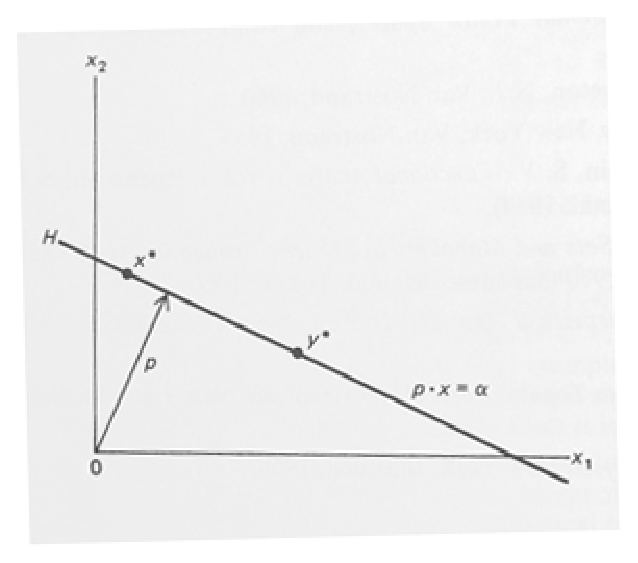
\includegraphics[width=0.47\textwidth]{line}}\hfill
\subfigure[Плоскость]{\includegraphics[width=0.47\textwidth]{3dplane}}
\caption{Примеры гиперплоскостей}\label{fig:Hplanes_exam}
\end{figure}



Изменяя значение $\gamma$ (сдвигая гиперплоскость), мы получаем
целое семейство гиперплоскостей (см. Рис.~\ref{fig:hypermap}).

\input{pics/hypermap.TpX}


    Важнейшая роль выпуклых множество в математической экономике и теории экстремальных задач
    обусловлена тем, что для них справедливы так называемые теоремы отделимости.
    Есть несколько различных формулировок теорем отделимости. Мы приведем здесь только те из них,
    которые понадобятся нам в дальнейшем. Их доказательства мы приводить не будем в надежде на то,
    что геометрически они выглядят довольно правдоподобными.

    Два множества $\st{X}$ и $\st{Y}$ из $\R^n$ называются
    \emph{отделимыми}, если существует такая гиперплоскость
    $\st{H}_{p,\gamma}$, называемая \emph{разделяющей}, что множество
    $\st{X}$ лежит в одном
    из замкнутых полупространств, порожденных этой гиперплоскостью,
    а множество $\st{Y}$ --- во втором. Иными словами, множества $\st{X}$ и
    $\st{Y}$ отделимы, если существуют такой ненулевой линейный функционал $p(\vc{x})$,
    и число $\gamma$, что
\[
    p(\vc{x})\leq\gamma\leq p(\vc{y}) \ \forall \vc{x}\in\st{X} \ \forall \vc{y}\in\st{Y}.
\]




\begin{teo}[отделимости]
  \label{teo-otd-1}
    Предположим, что $\st{X}$ и $\st{Y}$ --- выпуклые множества из
    $\R^n$, причем хотя бы одно из них, скажем, $\st{Y}$, имеет
    непустую внутренность (\remrk{что такое внутренность????}) $\emph{int}\st{Y}$. Если
    $\st{X}\cap\emph{int}\st{Y}=\emptyset$, то множества $\st{X}$ и
    $\st{Y}$ отделимы.
\end{teo}

     Подчеркнем, что в
    сформулированной теореме не требуется, чтобы множества не пересекались. Важно, чтобы
    одно из двух множеств не пересекалось с внутренностью другого, если, конечно, эта
    внутренность сама не являлась пустым множеством (см. \remrk{РИС}).
    Безусловно, предположение о том, что оба множества, $\st{X}$ и $\st{Y}$,
    являются выпуклыми, является крайне существенным, что проиллюстрировано \remrk{РИС}.


    Пусть $\st{X}$ --- некоторое множество из $\R^{n}$ и точка
    $\vc{\hat{x}}$ принадлежит границе этого множества. Гиперплоскость
    $\st{H}_{p,\gamma}$ называется \emph{опорной} к множеству $\st{X}$
    в точке $\vc{\hat{x}}$, если эта точка принадлежит
    данной гиперплоскости, а само множество $\st{X}$ содержится в
    полупространстве $\st{H}_{p,\gamma}^{-}$, т.е. если
    \[\gamma=p(\vc{\hat{x}})\geq p(\vc{x}) \ \forall x\in\st{X}.\]

    Заметим, что последнее неравенство говорит, в частности, что
    если точка $\vc{\hat{x}}$  принадлежит множеству $\st{X}$
    (а это действительно так, если это множество замкнуто),
    то она  представляет собой решение задачи
\begin{equation}
    \label{max-lin-na-vip}
    p(\vc{x})\rightarrow\max, \ \vc{x}\in\st{X},
\end{equation}
    причем значением этой задачи является число $\gamma$. Подчеркнем также,
    что, формально говоря, опорная к множеству $\st{X}$
    в точке $\vc{\hat{x}}$ гиперплоскость представляет собой
    гиперплоскость, разделяющую множество $\st{X}$ и множество,
    состоящее из единственной точки $\vc{\hat{x}}$ (\remrk{РИС}).

\begin{teo}[об опорной гиперплоскости]
    \label{teo-op-gip}
    Если $\st{X}$ --- выпуклое множество, то для любой его граничной (\remrk{????})
    точки $\vc{\hat{x}}$  найдется гиперплоскость, опорная в этой точке
    к данному множеству.
\end{teo}

    Из теоремы об опорной гиперплоскости следует, что любая
    граничная точка выпуклого замкнутого множества $\st{X}$ представляет
    собой решение некоторой задачи вида (\ref{max-lin-na-vip}). В то
    же время, очевидно, что любое решение такой задачи является
    граничной точкой $\st{X}$. Заметим, что в случае, когда
    множество $\st{X}$ имеет непустую внутренность, теорема об
    опорной гиперплоскости вытекает из теоремы отделимости.

    Далее нам понадобится еще одна теорема, которая говорит, что
    если точка $\vc{\hat{x}}$ не принадлежит выпуклому замкнутому
    множеству $\st{X}$, то $\vc{\hat{x}}$ <<строго>> отделима от
    $\st{X}$ с помощью некоторой гиперплоскости $\st{H}_{p,\gamma}$ (\remrk{РИС ?????}).


\begin{teo}\label{strog-otdotochki}
    Пусть $\st{X}$ --- выпуклое замкнутое множество, а точка
    $\vc{\hat{x}}$  не принадлежит $\st{X}$. Тогда существует такой
    ненулевой линейный функционал $p(\vc{x})$ и число
     $\gamma$, такие что
    \[p(\vc{x})<p(\vc{\hat{x}}) \ \forall \vc{x}\in\st{X}.\]
\end{teo}

\begin{exer}
    Докажите, что любое замкнутое выпуклое множество $\st{X}$ представляет
    собой пересечение всех полупространств
    $\st{H}_{p,\gamma}^{-}$, порождаемых опорными к $\st{X}$
    гиперплоскостями.


\end{exer}


\section{Лемма Фаркаша}

    В качестве приложения одной из только что сформулированных теорем, докажем важную
    лемму Фаркаша, которую мы уже использовали в предыдущей главе для доказательства
    некоторых теорем линейного программирования.


    Множество $\st{X}\subset\R^{n}$ называется \emph{\textbf{конусом}}, если для
    любого вектора $\vc{x}\in\st{X}$ и любого числа
    $\lambda\geqslant0$ справедливо включение
     $\lambda\vc{x}\in\st{X}$, т.е. если вместе с любой своей точкой множество
     $\st{X}$ вместе с любой своей точкой содержит проходящий через
     нее луч с началом в нуле (см. рис. ?????, а)
     Если конус $\st{X}$ является выпуклым
     множеством, то он называется \emph{\textbf{выпуклым конусом}} (см. рис. ?????, b).
     Простейшим примером выпуклого конуса является множество $\R_{+}^{n}$.


\begin{exer}
    Докажите, что
    \begin{itemize}
      \item множество $\st{X}$ является выпуклым конусом
    тогда и только тогда, когда для любых векторов $\vc{x'}\in\st{X}$
    и $\vc{x''}\in\st{X}$ и любых чисел $\lambda'\geqslant0$ и
    $\lambda''\geqslant0$ справедливо включение
    $\lambda'\vc{x'}+\lambda''\vc{x''}\in\st{X}$;
      \item пересечение любого числа выпуклых конусов является выпуклым
      конусом;
      \item объединение любого числа выпуклых конусов является конусом,
      но необязательно выпуклым.
    \end{itemize}

\end{exer}


    Пусть $\vc{a^{1}},\ldots,\vc{a^{m}}$ --- конечный набор векторов из
    $\R^{n}$. Вектор вида
    \[\lambda_{1}\vc{a^{1}}+\ldots+\lambda_{m}\vc{a^{m}}\] называется
    \textbf{\emph{линейной комбинацией}} этих векторов. Эта
    линейная комбинация называется \emph{\textbf{неотрицательной}}, если
    $\lambda_{1}\geqslant0,\ldots,\lambda_{m}\geqslant0$ и \emph{\textbf{выпуклой}},
    если $\lambda_{1}\geqslant0,\ldots,\lambda_{m}\geqslant0$ и
    $\lambda_{1}+\ldots+\lambda_{m}=1$. Напомним, что понятие выпуклой комбинации двух точек
    мы уже использовали.




\begin{exer}\label{vipukl-konus}
    Докажите, что
\begin{itemize}
      \item
      множество всевозможных неотрицательных линейных комбинаций конечного набора
      векторов является выпуклым конусом;
      \item
      множество всевозможных выпуклых комбинаций конечного набора
      векторов является выпуклым множеством;
 \end{itemize}
\end{exer}

    Множество всевозможных линейных неотрицательных комбинаций
    конечного набора векторов $\vc{a^{1}},\ldots,\vc{a^{m}}$
    называется конусом, \emph{\textbf{натянутым}} на эти вектора.


    Для доказательства леммы Фаркаша нам понадобится следующая
    техническая лемма. Доказательство этой леммы является несложным, но
    довольно длинным. Поэтому мы его опускаем в надежде на то, что
    сама ее формулировка представляется читателю вполне
    естественной.

\begin{lem}\label{zamkn-konus}
    Конус, натянутый на любой конечный набор векторов, является
    замкнутым множеством.
\end{lem}


    Перейдем к формулировке и доказательству леммы Фаркаша.


\begin{teop}(лемма Фаркаша) \label{lemma-F1}
    Предположим, что нам задан конечный набор векторов
    \[\vc{a_{1}},\ldots,\vc{a_{m}},\]
    лежащих в конечномерном пространстве ${\R}^{n}$. Для любого
    вектора $\vc{d}$ из ${\R}^{n}$ справедлива одна и только одна из двух
    следующих альтернатив:
\begin{itemize}
    \item [1)\ ] либо найдутся числа
    $v_{1}\geq0,\ldots,v_{m}\geq0$, такие что
    \[\vc{d}=v_{1}\vc{a_{1}}+\ldots+v_{m}\vc{a_{m}};\]

    \item [2)\ ] либо существует такой линейный функционал $h(\cdot)$,
    заданный на ${\R}^{n}$, что одновременно выполняются следующие неравенства:
    \[h(\vc{a_{1}})\leq0,\ldots,h(\vc{a_{m}})\leq0,\]
    \[h(\vc{d})>0.\]
\end{itemize}
\end{teop}

    \emph{\textbf{Доказательство.}}
    Рассмотрим конус $\mathbb{K}$, натянутый на вектора
    $\vc{a_{1}},\ldots,\vc{a_{m}}$. Этот конус является выпуклым
    (см. упражнение \ref{vipukl-konus}) и, по
    лемме \ref{zamkn-konus}, замкнутым.

    Возможно одно и только одно из двух следующих соотношений: либо $\vc{d}\in\mathbb{K}$,
    либо $\vc{d}\notin\mathbb{K}$. Включение  $\vc{d}\in\mathbb{K}$
    эквивалентно существованию (\remrk{РИС ?????}) таких неотрицательных чисел
    $v_{1}\geq0,\ldots,v_{m}\geq0$, что
    \[\vc{d}=v_{1}\vc{a_{1}}+\ldots+v_{m}\vc{a_{m}}.\]

    Что касается соотношения $\vc{d}\notin\mathbb{K}$, то с учетом
    теоремы \ref{strog-otdotochki}, оно эквивалентно существованию
    такого линейного функционала $h(\vc{x})$ (\remrk{РИС ?????}), заданного на пространстве $\R^{n}$,
    для которого выполняется следующее соотношение:
\[
    h(\vc{x})< h(\vc{d}) \ \forall \vc{x}\in\mathbb{K}.
\]
    Поскольку $\vc{0}\in\mathbb{K}$, мы имеем: $h(\vc{d})>0$.

    Покажем, что
\[
    h(\vc{x})\leqslant0 \ \forall \vc{x}\in\mathbb{K}.
\]
    Действительно, предположим, что $h(\vc{\bar{x}})>0$ для некоторого
    $\vc{\bar{x}}\in\mathbb{K}$. В этом случае при достаточно
    большом $\lambda>0$ одновременно выполняется неравенство
    $h(\lambda\vc{\bar{x}})>h(\vc{d})$ и включение
    $\lambda\vc{\bar{x}}\in\mathbb{K}$, чего быть не может.

    Нам осталось заметить, что $\vc{a_{j}}\in\mathbb{K}, \ j=1,\ldots,m$ и, значит,
    $h(\vc{a_{j}})\leqslant0, \ j=1,\ldots,m$.
    $\Box$

    Важным следствием доказанной теоремы является следующая лемма.

\begin{lem}\label{lemma-F2}
    Предположим, что нам заданы $r\times s$ матрица $\vc{A}$ и
    $r$-мерный вектор-столбец $\vc{d}$. Справедлива ровно одна из двух
    следующих альтернатив:
\begin{itemize}
    \item [1)\ ] либо найдется $s$-мерный вектор-столбец $\vc{v}\geqq\vc{0}$,
    такой что
    \[\vc{d}=\vc{A}\vc{v};\]

    \item [2)\ ] либо существует такая вектор-строка $\vc{h}$, что
    одновременно выполняются следующие неравенства:
    \[\vc{h}\vc{A}\leqq0, \ \vc{h}\vc{d}>0.\]
    \end{itemize}
\end{lem}
    \textbf{\emph{Доказательство.}}
    Рассмотрим набор $r$-мерных
    вектор-столбцов $\vc{a_{1}},\ldots,\vc{a_{s}}$,  из которых состоит матрица
    $\vc{A}$, и $r$-мерный вектор-столбец $\vc{d}$. По теореме
    \ref{lemma-F1} выполняется ровно одна из двух следующих
    альтернатив:

    --- либо существует такой неотрицательный $s$-мерный
    вектор-столбец
    $\vc{v}=\left(
              \begin{array}{c}
                v_{1} \\
                \vdots \\
                v_{s} \\
              \end{array}
            \right)$,
            что
       \[\vc{d}=v_{1}\vc{a_{1}}+\ldots+v_{s}\vc{a_{s}}=\vc{A}\vc{v},\]
    --- либо найдется такой линейный функционал $h(\vc{x})$,
    заданный на ${\R}^{r}$, что одновременно выполняются следующие неравенства:
    \[h(\vc{d})>0,\]
  \[h(\vc{a_{1}})\leq0,\ldots,h(\vc{a_{m}})\leq0.\]
    Рассмотрим вторую альтернативу.
    Как мы помним, всякий линейный функционал, заданный на пространстве
    $\R^{r}$, состоящем из вектор-столбцов, однозначным образом
    задается некоторой $r$-мерной вектор-строкой. Применительно к
    линейному функционалу $h(\vc{x})$ это значит, что существует
    такая вектор-строка $\vc{h}=(h_{1},\ldots,h_{r})$, что для любого
    вектора $\vc{x}\in\R^{r}$ выполняется равенство
    $\vc{h}\vc{x}=h(\vc{x})$. Для этой вектор-строки мы имеем:
\[
    \vc{h}\vc{d}>0,
\]
\[
    \vc{h}\vc{a_{1}}\leq0,\ldots,\vc{h}\vc{a_{s}}\leq0,
\]
    причем последний набор неравенств мы компактно можем переписать
    в следующем виде:
\[
    \vc{h}\vc{A}\leqq0. \Box
\]

\begin{exer}
    Докажите следующую лемму.
\end{exer}


\begin{lem}\label{lemma-F3}
    Предположим, что нам заданы $s\times r$ матрица $\vc{A}$ и
    $r$-мерный вектор-столбец $\vc{d}$. Справедлива ровно одна из двух
    следующих альтернатив:
\begin{itemize}
    \item [1)\ ] либо найдется $s$-мерный вектор-строка $\vc{v}\geqq\vc{0}$,
    такая что
    \[\vc{d}=\vc{v}\vc{A};\]

    \item [2)\ ] либо существует такой вектор-столбец $\vc{h}$, что
    одновременно выполняются следующие неравенства:
    \[\vc{A}\vc{h}\leqq0, \ \vc{d}\vc{h}>0.\]
    \end{itemize}
\end{lem}

    Заметим, что в научной и учебной литературе иногда под леммой Фаркаша понимают не теорему
    \ref{lemma-F1}, а лемму \ref{lemma-F2} или лемму \ref{lemma-F3}










\newpage

\section{Эффективные точки}

Важную роль в экономическом анализе играет понятие эффективности,
которое несколько отличается от обыденного представления об
эффективности.


УТОЧНИТЬ ОПРЕДЕЛЕНИЯ!!!!!

\begin{dfn}

    Точка ${\vc{\hat x}} \in \st{X} \subset \R^n$ называется

\begin{enumerate}
  \item \textbf{эффективной} точкой множества $\st{X}$, если не существует другой точки $\vc{x} \in
\st{X}$, такой, что $\vc{x} \geq \vc{\hat x}$;

  \item \textbf{слабо эффективной} точкой
множества $\st{X}$, если не существует другой точки $\vc{x} \in
\st{X}$, такой, что $\vc{x} \gg \vc{\hat x}$.

\end{enumerate}
\end{dfn}

    Чтобы пояснить введенные определения, напомним, какой смысл
    имеют неравенства $\geq$ и $\gg$ применительно к векторам. Для
    векторов $\vc{x}=(x_{1},...,x_{n})$ и $\vc{y}=(y_{1},...,y_{n})$
    из пространства $\R^{n}$ неравенство $\vc{x}\gg\vc{y}$
    означает, что
\[
    x_{i}>y_{i}, \ i=1,...,n,
\]
    неравенство $\vc{x}\geqq\vc{y}$ говорит о том, что
\[
    x_{i}\geqslant y_{i}, \ i=1,...,n,
\]
    а соотношение $\vc{x}\geq\vc{y}$ --- о том, что выполняются последние неравенства и $x_{i}>y_{i}$
    хотя бы для одного $i$.
    Мы видим, что точка
    ${\vc{\hat x}} \in \st{X}$ является слабо эффективной, если \emph{не
    найдется} другой точки $\vc{x}$ из множества $\st{X}$,
    превосходящей ${\vc{\hat x}}$ по всем координатам. Точка
    ${\vc{\hat x}} \in \st{X}$ является эффективной, если не найдется другой
    точки $\vc{x}\in\st{X}$, которая не меньше ${\vc{\hat x}}$ по
    всем координатам, причем хотя бы по одной --- строго больше.






Из приведенного выше определения нетрудно видеть, что любая эффективная точка является и
слабо эффективной. Если точка не является слабо эффективной, то она не может быть и
эффективной. В то же время, из того факта, что точка ${\vc{\hat x}}$ является слабо
эффективной, не следует, что она эффективна. (\remrk{РИС?????})





\begin{prop}\label{vzvesh-summa}

Пусть $\st{X} \subset \R^n$ и пусть вектор $\vc{\hat x}$ представляет собой решение задачи

\begin{equation}\label{eq:eff_conditions}
\left\{ \begin{array}{l}
 \vc{p}\vc{x} = p_1x_1 + \ldots + p_n x_n\to \max  \\
 \vc{x} \in \st{X}, \\
 \end{array} \right.
\end{equation}



\begin{enumerate}
\renewcommand{\theenumi}{(\roman{enumi})}
  \item Если $\vc{p} \geq \vc{0}$, то точка $\vc{\hat x} \in \st{X}$ является
  слабо эффективной.
  \item Если $\vc{p} \gg \vc{0}$, то точка $\vc{\hat x} \in \st{X}$ является
  эффективной.
\end{enumerate}

\end{prop}

\begin{proof}

(i) Предположим, что утверждение данного пункта не выполняется. В
этом случае существует $\vc{\bar x} \in \st{X}$ такой, что $\vc{\bar
x} \gg \vc{\hat x}$. Тогда, поскольку $\vc{p} \geq \vc{0}$, получаем
$\vc{p}\vc{\bar x} > \vc{p}\vc{\hat x}$. Однако это противоречит
тому факту, что $\vc{\hat x}$ есть решение задачи
(\ref{eq:eff_conditions}).

(ii) Докажите самостоятельно в качестве \textbf{упражнения}.

\end{proof}



Отметим, что в приведенном предложении не накладывается никаких требований к устройству
множества $\st{X}$. В некотором смысле обратное утверждение требует выпуклости множества
$\st{X}$.



\begin{prop}\label{usl-eff}

Пусть $\st{X} \subset \R^n$ --- выпуклое множество. Если точка ${\vc{\hat x} \in \st{X}}$
является слабо эффективной точкой множества $\st{X}$, то существует вектор ${\vc{p} \geq
\vc{0}}$ из $\R^n$, такой что
\[\vc{p}\vc{\hat x}\geq\vc{p}\vc{x} \ \forall \vc{x}\in\st{X},\]
т.е. $\vc{\hat x}$ есть решение задачи (\ref{eq:eff_conditions}).
\end{prop}

\begin{proof}
Положим
\[
    \st{Y}=\{\vc{y} \in \R^n: \vc{y} \geqq \vc{\hat x}\}.
\]
Множество $\st{Y}$ является выпуклым, причем, как легко проверить,
\[
    \text{int}\st{Y}=\{\vc{y} \in \R^n: \vc{y} \gg \vc{\hat x}\}.
\]

 Поскольку $\vc{\hat x}$
является слабо эффективной точкой множества $\st{X}$, то, как легко заметить,
 $\st{X}\cap\text{int}\st{Y}=\emptyset$. Таким образом, мы имеем два непересекающихся
 выпуклых множества, $\st{X}$ и $\st{Y}$, причем таких, что первое из них не пересекается
 с непустой внутренностью второго (\remrk{РИС?????}).

Значит, по теореме отделимости (теореме \ref{teo-otd-1}) найдутся
ненулевой вектор $\vc{p}=(p_{1},...,p_{n})\in \R^n$ и число
    $\gamma\in \R$ такие, что для любого $\vc{x} \in \st{X}$ и любого $\vc{y}
\in \st{Y}$ выполняются следующие соотношения:

\[
\vc{p} \cdot \vc{x} \leq \gamma \leq \vc{p} \cdot \vc{y}.
\]

    Проверим, что $\vc{p} \geq \vc{0}$. Для этого предположим, что
 это не так и, тем самым, $p_i <0$ для некоторого $i$. Обозначим
 через $\vc{e_{i}}$ вектор из $\R^{n}$, все координаты
 которого, за исключением $i$-й, равны $0$, а $i$-я координата равна
 $1$. Очевидно, $\vc{p}\vc{e_{i}}=p_{i}<0$
    и, следовательно, $\vc{p}(\vc{\hat x}+\vc{e_{i}})<\vc{p}\vc{\hat x}$.
    А этого быть не может, поскольку вектор $\vc{\hat x}+\vc{e_{i}}$ содержится в $\st{Y}$.

    Нам осталось заметить, что, поскольку $\vc{\hat x}$ содержится как в $\st{X}$, так и в
    $\st{Y}$, мы имеем
    $\vc{p} \cdot \vc{\hat x}=\gamma$.
    А это означает, что
    $\vc{\hat x}$ есть решение задачи (\ref{eq:eff_conditions}).
\end{proof}

    Из двух сформулированных предложений вытекает следующая теорема.

\begin{teop}\label{neob-dosti-usl-eff}
    Пусть $\st{X} \subset \R^n$ --- выпуклое замкнутое множество.
    Вектор ${\vc{\hat x} \in \st{X}}$ является слабо эффективной точкой
    множества $\st{X}$ тогда и только тогда, когда то существует вектор
    ${\vc{p} \geq \vc{0}}$, $\vc{p} \in \R^n$, такой что
    \[\vc{p}\vc{\hat x}\geq\vc{p}\vc{x} \ \forall \vc{x}\in\st{X},\]
    т.е. $\vc{\hat x}$ есть решение задачи (\ref{eq:eff_conditions}).
\end{teop}



  Напомнив, что всякая эффективная точка
  является и слабо эффективной, отметим, что нельзя сформулировать аналогичные
  необходимые и достаточные условия эффективности.
  Действительно, из того факта, что точка
  является эффективной, вовсе не следует, что соответствующий вектор $\vc{p} \gg \vc{0}$. В
  качестве примера на Рис.~\ref{fig:circle_eff} приведем окружность (выпуклое
  множество), точка $A$ которой очевидным образом является
  эффективной, но $\vc{p} \geq \vc{0}$. (В качестве \textbf{упражнения}
  аккуратно докажите этот факт).

\input{pics/circle_eff.TpX}




\begin{exer}
  \label{neper-pol-ort}
    Докажите, что выпуклое множество $\st{X}$ не пересекается с множеством
    $\{\vc{x}\in \R^{n} \mid  \vc{x}\gg \vc{0} \}$ тогда и только тогда, когда существует
    вектор
    ${\vc{p} \geq \vc{0}}$, $\vc{p} \in \R^n$, такой что
\[
    \vc{p}\vc{x}\leq 0 \ \forall \vc{x}\in \st{X}.
\]


\end{exer}

\begin{exer}
    Пусть
    $\st{X}=\{\vc{x}=(x_{1},x_{2})\in\R_{+}^{2}\mid
    x_{1}^{2}+x_{2}^{2}\leqslant25\}$,
    $\vc{\hat{x}}=(3,4)$. Докажите, что точка $\vc{\hat{x}}$
    эффективна и укажите коэффициенты $p_{1}$ и $p_{2}$ при которых
    эта точка является решением задачи (\ref{eq:eff_conditions}).


\end{exer}






Стандартный пример выпуклого множества, приводимый в элементарных учебниках по экономической
теории --- множество производственных возможностей экономики, ограниченное \dw{кривой
производственных возможностей} (англ., \emph{production possibility
frontier}\footnote{\cite{McConnell:1996}}). См. Рис.~\ref{fig:ppfrontier}, где изображены
множество производственных возможностей и граница производственных возможностей экономики,
производящей два вида товаров: пушки и масло. Граница производственных возможностей --- это,
как уже заметил читатель, множество всех слабо эффективных точек множества производственных
возможностей. Теорема \ref{neob-dosti-usl-eff} применительно к данному примеру говорит о том,
что некоторый вектор выпускаемых продуктов принадлежит границе производственных возможностей
тогда и только тогда, когда этот вектор доставляет максимум валового внутреннего продукта на
всем множестве производственных возможностей экономики при некотором векторе цен на
выпускаемые продукты. Очевидно, что разным векторам цен соответствуют, вообще говоря,
различные точки на границе производственных возможностей.


\input{pics/ppfrontier.TpX}


Рис.~\ref{fig:ppfrontier} \emph{а)},

На Рис.~\ref{fig:ppfrontier} \emph{б)}  Рис.~\ref{fig:ppfront_max}.

\input{pics/ppfront_max.TpX}






\subsection{Выпуклые и вогнутые функции}

    Теперь перейдем к описанию основных свойств выпуклых и вогнутых функций, которые играют
    ключевую роль в математической экономике и экономической теории в целом.


\begin{dfn}
Пусть нам дано выпуклое множество $\st{X} \subset \R^n$. Функция
    $f: \st{X} \to \R$ называется

\begin{enumerate}
\renewcommand{\theenumi}{(\asbuk{enumi})}

  \item  \dw{вогнутой}\index{вогнутая функция},
если для любых $\vc{x}', \vc{x}'' \in \st{X}$ и $0 \leq \theta \leq
1$ выполняется (см. Рис. \ref{fig:concave-function})

\[
    f[\theta \vc{x}' + (1-\theta)\vc{x}'] \geq \theta f(\vc{x}') +
    (1-\theta)f(\vc{x}'').
\]

  \item \dw{строго вогнутой}\index{строго вогнутая функция},
если для любых $\vc{x}', \vc{x}'' \in \st{X}$, $\vc{x}' \neq
\vc{x}''\!$, и $0 < \theta < 1$ выполняется

\[
f[\theta \vc{x}' + (1-\theta)\vc{x}''] > \theta f(\vc{x}') +
(1-\theta)f(\vc{x}'').
\]

  \item \dw{выпуклой}\index{выпуклая функция},
если для любых $\vc{x}', \vc{x}'' \in \st{X}$ и $0 \leq \theta \leq
1$ выполняется

\[
f[\theta \vc{x}' + (1-\theta)\vc{x}''] \leq \theta f(\vc{x}') +
(1-\theta)f(\vc{x}'').
\]

\item \dw{строго выпуклой}\index{строго выпуклая функция},
если для любых $\vc{x}', \vc{x}'' \in \st{X}$, $\vc{x}' \neq
\vc{x}''\!$, и $0 < \theta < 1$ выполняется

\[
f[\theta \vc{x}' + (1-\theta)\vc{x}''] < \theta f(\vc{x}') +
(1-\theta)f(\vc{x}'').
\]

\end{enumerate}
\end{dfn}


\begin{figure} \centering
   \includegraphics[width=10cm]{concave_function}\\
  \caption{Вогнутая функция}\label{fig:concave-function}
\end{figure}


    \remrk{НА РИС} изображены строго выпуклая и строго вогнутая функции, а выпуклая функция,
    не являющаяся строго выпуклой, и вогнутая функция, не являющаяся строго вогнутой.



\begin{dfn}
    Пусть $\st{X}\subset\R^{n}$.
 \dw{Надграфиком} функции $f:\st{X}\rightarrow \R$ называется множество
    \[
    \st{G}_{f}^+=\{ (\vc{x}, \gamma) \in \R^{n+1}: \vc{x}\subset\st{X}, \
    f(\vc{x}) \leq \gamma \},
    \]
    а \dw{подграфиком} --- множество
    \[
    \st{G}_{f}^- =\{ (\vc{x}, \gamma) \in \R^{n+1}: \vc{x}\subset\st{X}, \
    f(\vc{x}) \geq \gamma \}.
    \]
\end{dfn}

\remrk{? Как обозначить лебегово множество}



\begin{exer}
Докажите следующие утверждения.


\begin{enumerate}
\renewcommand{\theenumi}{(\roman{enumi})}

  \item Функция $f(\vc{x})$ является выпуклой
(строго выпуклой) тогда и только тогда, когда функция $-f(\vc{x})$
является вогнутой (строго вогнутой).

  \item Линейная функция является и вогнутой, и выпуклой, но не является строго вогнутой или
  строго выпуклой.

  \item
  Если функции $f_{j}(\vc{x}), \ j=1,...,m,$ вогнуты (выпуклы), то
  при любых неотрицательных числах $\lambda_{1},...,\lambda_{m}$
  вогнута (выпукла) и функция
  $f(\vc{x})=\lambda_{1}f_{1}(\vc{x})+...+\lambda_{m}f_{m}(\vc{x})$
  (неотрицательная линейная комбинация вогнутых функций также
  вогнута, а выпуклых --- выпукла).


  \item Функция является выпуклой (вогнутой) тогда и только тогда,
  когда ее надграфик (подграфик) является выпуклым множеством.

  \item Функция $f(\vc{x})$, заданная на выпуклом множестве $\st{X}$,
  является выпуклой (вогнутой) тогда и только тогда,
  когда для любого целого числа $m \geq 1$, для любых векторов
  $\vc{x}^j \in \st{X}, \ j=1,..,m,$ и любых таких неотрицательных чисел
  $\theta_j \geq 0, \ j=1,\ldots,m,$ что
  $\theta_{1}+...+\theta_{m}=1$, выполняется \emph{неравенство Йенсена}:
  \[
    f(\theta_1 \vc{x}^1 +...+\theta_m
    \vc{x}^m) \leq \theta_1 f(\vc{x}^1)+\ldots +\theta_m
    f(\vc{x}^m)
  \]
  \[
    (f(\theta_1 \vc{x}^1 +...+\theta_m
    \vc{x}^m) \geq \theta_1 f(\vc{x}^1) + \ldots +\theta_m
    f(\vc{x}^m))
  \]

    \item Функция $f:\st{X}\rightarrow \R$ является вогнутой тогда и только тогда, когда
    выпуклым является множество
\[
    \st{G}_{f}^+=\{ (\vc{x}, \gamma) \in \R^{n+1}: \vc{x}\subset\st{X}, \
    f(\vc{x}) \leq \gamma \},
\]
    (оно называется надграфиком функции $f$)

    \item Функция $f:\st{X}\rightarrow \R$ является выпуклой тогда и только тогда, когда
    выпуклым является множество
\[
    \st{G}_{f}^- =\{ (\vc{x}, \gamma) \in \R^{n+1}: \vc{x}\subset\st{X}, \
    f(\vc{x}) \geq \gamma \}.
\]
    (оно называется подграфиком функции $f$)

  \item Если функции $f_{j}(\vc{x}), \ j=1,...,m,$ являются
  выпуклыми, то функция
  $f(\vc{x})=\min\limits_{j}f_{j}(\vc{x})$
  тоже выпукла.
  Если функции $f_j (\vc{x}), j=1, \ldots, m$, являются
  вогнутыми, то функция
  $f(\vc{x}) = \mathop {\min }\limits_j f_j(\vc{x})$ также вогнута.

\end{enumerate}

\end{exer}

\remrk{ПЕРЕНЕСТИ В СЛЕД ГЛАВУ:}

\remrk{Следующее предложение иллюстрируется РИС???}



\begin{prop}
    Если в некоторой точке $\vc{\hat x}$ выпуклого множества $\st{X}$
    достигается локальный максимум (минимум) вогнутой  (выпуклой)
    функции $f(\vc{x})$, то в этой же
  точке достигается и глобальный максимум  (минимум).
\end{prop}
    \textbf{Доказательство.} Мы проведем доказательство для случая локального
    максимума вогнутой функции. Пусть $\vc{\hat x}$ --- точка
    локального максимума. Это означает, что существует такая
    $\epsilon$-окрестность $\mathcal{U}_{\epsilon}(\vc{\hat x})$ ($\epsilon>0$) точки
    $\vc{\hat x}$, что
\[
    f(\vc{\hat x})\geqslant f(\vc{x}) \
    \forall \vc{x}\in\st{X}\cap\mathcal{U}_{\epsilon}(\vc{\hat x})
\]
    Возьмем произвольную точку $\vc{x}\in\st{X}$. Поскольку и
    $\vc{\hat x}$, и $\vc{x}$ принадлежит множеству $\st{X}$, причем
    это множество выпукло,
\[
    \vc{\bar{x}}=(1-\lambda)\vc{\hat{x}}+\lambda\vc{x}
    \in\st{X}\cap\mathcal{U}_{\epsilon}(\vc{\hat x})
\]
    при достаточно малом $\lambda>0$ и, следовательно, с учетом
    определения вогнутой функции,
\[
    f(\vc{\hat{x}})\geqslant f(\vc{\bar{x}})= f((1-\lambda)\vc{\hat{x}}+\lambda\vc{x})
    \geqslant(1-\lambda)f(\vc{\hat{x}})+\lambda f(\vc{x}),
\]
    откуда вытекает неравенство $\lambda f(\vc{\hat{x}})\geqslant \lambda f(\vc{x}).$

    Тем самым, с учетом произвольности выбора точки $\vc{x}$,
\[
    f(\vc{\hat{x}})\geqslant f(\vc{x}) \ \forall \vc{x}\in\st{X},
\]
    что и требуется. $\Box$

\remrk{Следующее предложение иллюстрируется РИС???}

\begin{prop}
    Предположим, что функция $f(\vc{x})$ задана на выпуклом множестве
    $\st{X}$  и дифференцируема в точке $\vc{\hat x} \in \st{X}$.
    Если функция $f(\vc{x})$ выпукла, то
\[
    f(\vc{x}) \geqslant f(\vc{\hat x}) + \nabla f(\vc{\hat x}) \cdot
    (\vc{x}-\vc{\hat x}) \ \forall \vc{x} \in  \st{X},
\]
    а если вогнута, то
\[
    f(\vc{x}) \leqslant f(\vc{\hat x}) + \nabla f(\vc{\hat x}) \cdot
    (\vc{x}-\vc{\hat x}) \ \forall \vc{x} \in  \st{X}.
\]
\end{prop}
    \textbf{Доказательство.} Мы рассмотрим случай, когда функция $f(\vc{x})$
    выпукла.
    Зафиксируем $\vc{x} \in  \st{X}$ и положим $\vc{h}=\vc{x}-\vc{\hat x}$.
    Поскольку множество $\st{X}$ выпукло, точка
    $\vc{\hat x}+\alpha\vc{h}=\alpha\vc{x}+(1-\alpha)\vc{\hat x}$
    принадлежит этому множеству при всех $\alpha\in(0,1)$. В силу
    дифференцируемости (\remrk{ЧТО ЕСТЬ ДИФФЕРЕНЦИРУЕМОСТЬ???}) функции $f(\vc{x})$  в точке $\vc{\hat x}$, при
    достаточно малых $\alpha\in(0,1)$ мы имеем:
\begin{multline*}
    f(\alpha\vc{x}+(1-\alpha)\vc{\hat x})
    =f(\vc{\hat x}+\alpha\vc{h})= \\
    =f(\vc{\hat x})+\nabla f(\vc{\hat x})(\alpha\vc{h})+o(\|\alpha\vc{h}\|)
    =f(\vc{\hat x})+\alpha\nabla f(\vc{\hat x})\vc{h}+o(\alpha)\|\vc{h}\|,
\end{multline*}
    а в силу выпуклости этой функции,
\[
    f(\alpha\vc{x}+(1-\alpha)\vc{\hat x})\leqslant
    \alpha f(\vc{x})+(1-\alpha)f(\vc{\hat x})
\]
    и, следовательно,
\[
    \alpha f(\vc{x})+(1-\alpha)f(\vc{\hat x})
    \geqslant f(\vc{\hat x})+\alpha\nabla f(\vc{\hat x})\vc{h}+o(\alpha)\|\vc{h}\|,
\]
    т.е.
\[
    \alpha(f(\vc{x})-f(\vc{\hat x}))
    \geqslant \alpha\nabla f(\vc{\hat x})(\vc{x}-\vc{\hat x})+o(\alpha)\|(\vc{x}-\vc{\hat x})\|.
\]
    Переходя в этом неравенстве к пределу при $\alpha\rightarrow 0$,
    получаем неравенство
\[
    f(\vc{x})-f(\vc{\hat x})\geqslant \nabla f(\vc{\hat x})(\vc{x}-\vc{\hat
    x}),
\]
    откуда и вытекает требуемое.    $\Box$

    Справедливо и в некотором смысле обратное утверждение, а именно,
    имеет место следующее предложение.

\begin{prop}
    Предположим, что функция $f(\vc{x})$ задана  на выпуклом открытом множестве
    $\st{X}$  и дифференцируема на этом множестве. Если для любых
    точек $\vc{x}$ и $\vc{y}$ из $\st{X}$ выполняется неравенство
\[
    f(\vc{x}) \geqslant f(\vc{y}) + \nabla f(\vc{y}) \cdot
    (\vc{x}-\vc{y}) \ \forall \vc{x} \in  \st{X},
\]
    то функция $f(\vc{x})$ выпукла, то а если неравенство
\[
    f(\vc{x}) \leqslant f(\vc{y}) + \nabla f(\vc{y}) \cdot
    (\vc{x}-\vc{y}) \ \forall \vc{x} \in  \st{X},
\]
    то вогнута. $\Box$
\end{prop}


\begin{exer}
    Докажите это предложение.
\end{exer}






\remrk{ПЕРЕНЕСТИ В СЛЕД ГЛАВУ:}



    Напомним, что, согласно теореме \ref{nul-grad-neobh}, если внутренняя точка
    $\vc{x^{*}}$ некоторого множества $\st{D}$ является точкой локального
    максимума или точкой локального минимума дифференцируемой функции $f(\vc{x})$,
    то выполняется равенство $\nabla f(\vc{x^{*}})=\vc{0}$. Из
    доказанного предложения вытекает, что равенство градиента нулю
    представляет собой и достаточное условия максимума в случае,
    когда функция $f(\vc{x})$ вогнута или минимума, если эта функция
    выпукла. А именно, как мы видим, имеет место следующая теорема.

\begin{teo}\label{grad-nul}
    Предположим, что $\st{D}\subset\R^{n}$ --- это выпуклое
    множество, а $\vc{x^{*}}$ --- его внутренняя точка. Предположим
    далее, что функция $f(\vc{x})$, заданная на $\st{D}$, дифференцируема в
    точке $\vc{x^{*}}$.

    Если функция $f(\vc{x})$ вогнута, то
    $\vc{x^{*}}$ представляет собой решение задачи
\[
    f(\vc{x})\rightarrow\max, \ \vc{x}\in\st{D},
\]
    тогда и только тогда, когда $\nabla f(\vc{x^{*}})=\vc{0}$.

    Если функция $f(\vc{x})$ выпукла, то
    $\vc{x^{*}}$ представляет собой решение задачи
\[
    f(\vc{x})\rightarrow\min, \ \vc{x}\in\st{D},
\]
    тогда и только тогда, когда $\nabla f(\vc{x^{*}})=\vc{0}$.
\end{teo}


    Вогнутые и выпуклые функции могут быть и недифференцируемыми. Что касается непрерывности,
    то следует помнить, что справедливо следующее предложение, которые мы приведем без
    доказательства.

\begin{prop}
    Если функция $f(\vc{x})$, заданная на выпуклом множестве $\st{X}$, выпукла или вогнута,
    то она непрерывна на внутренности $\text{\emph{int}}\st{X}$ этого множества.
\end{prop}

\subsection{Квазивыпуклость и квазивогнутость}

    Кроме выпуклых и вогнутых функций экономисту нужно уметь работать с квазивыпуклыми и
    квазивогнутыми функциями.


\begin{dfn}
 Функция $f(\vc{x})$, заданная на выпуклом множестве $\st{X} \in
  \R^n$, называется \dw{квазивогнутой}\index{квазивогнутая функция},
  если для любого $\gamma \in \R$ выпукло множество
\[
    \st{L}^{+}_{f,\gamma}=\{ \vc{x}\in\st{X}: f(\vc{x}) \geq \gamma\},
\]
    и \dw{квазивыпуклой}\index{квазивыпуклая функция},
  если для любого $\gamma \in \R$ выпукло множество
\[
    \st{L}^{-}_{f,\gamma}= \{ \vc{x}\in\st{X}: f(\vc{x}) \leq \gamma \}.
\]
\end{dfn}

    Множество $\st{L}^{+}_{f,\gamma}$, как и множества $\st{L}^{-}_{f,\gamma}$,
    иногда называют \emph{лебеговым множеством} функции $f$. Множество
\[
    \st{L}^{=}_{f,\gamma}= \{ \vc{x}\in\st{X}: f(\vc{x})=\gamma \},
\]
    называют \emph{множеством уровня}. В случае, когда $n=2$,
    множество уровня по понятным причинам называют \emph{линией уровня}.

\remrk{РИС, РИС}


\begin{exer}
Докажите следующие утверждения.


\begin{enumerate}
\renewcommand{\theenumi}{(\roman{enumi})}

  \item Функция $f(\vc{x})$ является квазивыпуклой
    тогда и только тогда, когда функция $-f(\vc{x})$ является
    квазивогнутой.

  \item Всякая выпуклая функция квазивыпукла, а всякая вогнутая ---
  квазивогнута. Обратное, вообще говоря, неверно.



  \item Если функции $f_{j}(\vc{x}), \ j=1,...,m,$ являются
  квазивыпуклыми, то функция
  $f(\vc{x})=\min\limits_{j}f_{j}(\vc{x})$
  тоже квазивыпукла.
  Если функции $f_j (\vc{x}), j=1, \ldots, m$, являются
  квазивогнутыми, то функция
  $f(\vc{x}) = \mathop {\min }\limits_j f_j(\vc{x})$ также квазивогнута.


  \item
  Если функции $f_{1}(\vc{x})$ и $f_{2}(\vc{x})$ квазивогнуты (квазивыпуклы), то
  из этого не следует, что функция
  $f(\vc{x})=f_{1}(\vc{x})+f_{2}(\vc{x})$
  тоже является квазивогнутой (квазивыпуклой).


  \item
  Функция $f(\vc{x})$, заданная на выпуклом множестве $\st{X} \subset
  \R^n$, является квазивыпуклой (квазивогнутой) тогда и только
  тогда, когда для любых векторов $\vc{x'}\in\st{X}$ и
  $\vc{x''}\in\st{X}$ и любого числа $\alpha\in[0,1]$ выполняется
  неравенство
\[
    f(\alpha\vc{x'}+(1-\alpha)\vc{x''})\leqslant\max\{f(\vc{x'}),f(\vc{x''})\}
\]
\[
    f(\alpha\vc{x'}+(1-\alpha)\vc{x''})\geqslant\min\{f(\vc{x'}),f(\vc{x''})\}.
\]

    \item
    Функция $f(x)$, заданная на некотором интервале $(a,b)$ числовой прямой
    $\R$ квазивогнута тогда и только тогда, когда она

    --- либо не убывает на этом промежутке,

    --- либо монотонно не возрастает,

    --- либо существует точка $\hat{x}\in(a,b)$, такая что на
    промежутке $(a,\hat{x}]$ она монотонно не убывает, а на
    промежутке $[\hat{x},b)$ монотонно не возрастает.

    \item Функция
\begin{multline*}
    F(x_{1},\ldots,x_{n})=ax_{1}^{\alpha_{1}}x_{2}^{\alpha_{2}}\ldots x_{n}^{\alpha_{n}}, \ a>0, \\
    \alpha_{1}>0, \ \alpha_{2}>0, \ldots, \alpha_{n}>0, \
    \alpha_{1}+\alpha_{2}+\ldots+\alpha_{n}>1,
\end{multline*}
    является квазивогнутой, но не является вогнутой.


\end{enumerate}


\end{exer}





\subsection{Производственные функции}

        Предположим, что некоторое предприятие производит ровно один вид
         продукции или что выпуск измеряется в денежном выражении.
         Предположим далее, что при производстве продукции необходимо использование
         $n$ различных факторов. В этом случае технологию предприятия удобно
          описывать с помощью производственной функции $F(\vc{x})=F(x_{1},x_{2},...,x_{n})$,
          где $\vc{x}=(x_{1},x_{2},...,x_{n})$. Эта функция показывает максимально возможное
           количество продукции, которое может в течение единичного промежутка времени
           произвести данное предприятие,
           если оно использует первый фактор в количестве $x_{1}$ единиц, второй
           фактор --- в количестве $x_{2}$ единиц, ..., $n$-й фактор --- в количестве $x_{n}$.

           Говоря о какой-нибудь производственной функции $F(\vc{x})$,
           обычно предполагают, и мы тоже будем
           это всегда делать, что она задается на
           множестве  $\R^{n}_{+}$ при некотором целом $n$, принимает
           неотрицательные значения, непрерывна, удовлетворяет равенству
           и \textbf{\emph{монотонно не убывает}} в следующем смысле:
\[
    \vc{x}\geqq\vc{y}\Rightarrow F(\vc{x})\geq F(\vc{y}).
\]
           Иногда (но не всегда) предполагают, что она
           \textbf{\emph{монотонно возрастает}} в следующем смысле:
\[
    \vc{x'}\gg\vc{x''}\Rightarrow F(\vc{x'})>F(\vc{x''}).
\]

\begin{exer}
    Докажите, что всякая монотонно возрастающая производственная
    функция монотонно не убывает.
\end{exer}



            Очень часто берут $n=2$ и используют производственные
            функции вида $F(K,L)$, где $K$ --- это используемый капитал, а $L$ --- это труд.
            Так описывают производственный сектор экономики при
            построении макроэкономических моделей.


             Чаще всего в экономических исследованиях используют производственные
             функции следующих видов:



\begin{multline*}
    F(\vc{x})=F(x_{1},x_{2},...,x_{n})=a_{1}x_{1}+a_{2}x_{2}+...+a_{n}x_{n},
    \\
    a_{1}\geq0,...,a_{n}\geq0, \ \sum_{i=1}^{n}a_{i}>0,
\end{multline*}
     --- линейная производственная функция;
\begin{multline*}
    F(\vc{x})=F(x_{1},x_{2},...,x_{n})=\min\{x_{1}/a_{1},x_{2}/a_{2},...,x_{n}/a_{n}\},     \\
    a_{1}\geq0,...,a_{n}\geq0, \ \sum_{i=1}^{n}a_{i}>0,
\end{multline*}
    --- леонтьевская производственная функция (функция Леонтьева);

\begin{multline*}
    F(\vc{x})=F(x_{1},x_{2},...,x_{n})=
    ax_{1}^{\alpha_{1}}x_{2}^{\alpha_{2}}\ldots x_{n}^{\alpha_{n}},
     \ a>0, \ \alpha_{1}>0,..., \alpha_{n}>0,
\end{multline*}
     --- функция Кобба-Дугласа;

\begin{multline*}
    F(\vc{x})=F(x_{1},x_{2},...,x_{n})
    =(a_{1}x_{1}^{\rho}+\ldots+a_{n}x_{n}^{\rho})^{\alpha/\rho},
    \\ 0\neq\rho<1, \ \alpha>0, \ a_{1}>0,...,a_{n}>0,
\end{multline*}
     --- функция постоянной эластичности замещения (constant elasticity of substitution, CES).



\begin{exer}
    Покажите, что для леонтьевской производственной функции $F(\vc{x})$ справедливо равенство
\[
    \st{L}^{+}_{F,\gamma}=\{\vc{x}\in\R^{n} \mid \vc{x}\geqq \gamma \vc{a}\}
\]
    где $\vc{a}=(a_{1},\ldots,a_{n})$, а саму функцию
    можно эквивалентным образом определить посредством равенства
    \[F(\vc{x})=\min\{\lambda \ | \lambda\vc{x}\geqq \vc{a}\}.\]
\end{exer}

\begin{exer}
    Предположим, что $n=2$. Нарисуйте линии уровня
\[
    \st{L}^{=}_{F,1}= \{ \vc{x}\in\st{X}: F(\vc{x})=1 \} \ \text{и} \
    \st{L}^{=}_{F,2}= \{ \vc{x}\in\st{X}: F(\vc{x})=2 \},
\]
    в случае, когда $F(\vc{x})$ --- это
\begin{enumerate}

\item
    леонтьевская функция, $a_{1}=2, \ a_{2}=3$;
\item
    функция Кобба-Дугласа, $a=1, \ \alpha_{1}=\alpha_{2}=1/2$;
\item
    CES-функция, $\rho=1/2, \ \alpha=1, \ a_{1}=a_{2}=1$;
\item
    CES-функция, $\rho=-1, \ \alpha=1, \ a_{1}=a_{2}=1$.





\end{enumerate}


\end{exer}


    Говорят, что производственная функция удовлетворяет свойству
    \emph{постоянной отдачи} от расширения масштаба производства, если
    \[F(\lambda\vc{x})= \lambda F(\vc{x})
    \ \forall \lambda\geqslant0, \forall \vc{x}\in\R_{+}^{n}.\]
    Такие функции называют также \emph{положительно однородными} (первой
    степени).
    Если для любого $\vc{x}\in\R_{+}^{n}$, такого что $F(\vc{x})>0$, выполняется соотношение
\[
    F(\lambda\vc{x})> \lambda F(\vc{x})
\]
    то говорят, что функция демонстрирует \emph{возрастающую отдачу} от
    расширения масштаба производства. Если же
    для любого $\vc{x}\in\R_{+}^{n}$, такого что $F(\vc{x})>0$, выполняется соотношение
\[
    F(\lambda\vc{x})< \lambda F(\vc{x})
\]
    то говорят, что функция обладает свойством \emph{убывающей отдачи} от расширения
    масштаба производства.

\begin{exer}
    Может ли демонстрировать возрастающую отдачу от расширения
    масштаба производства вогнутая или квазивогнутая
    производственная функция?

\end{exer}

        Чтобы объяснить эти определения, предположим, что что объем всех
        используемых факторов производства увеличивается
        на 20\%. В случае постоянной отдачи от расширения масштаба
        производства это приведет к 20\% увеличению выпуска. Если имеет
        место убывающая отдача от расширения масштаба производства,
        то выпуск увеличится меньше чем на 20\%, а если имеет место
        возрастающая отдача, то больше, чем на 20\%.


\begin{exer}
    Покажите, что если для производственной функции Кобба-Дугласа
    выполняется равенство
     \[\alpha_{1}+\alpha_{2}+...+\alpha_{n}=1,\]
    то функция демонстрирует постоянную отдачу от расширения масштаба
    производства, если
     \[\alpha_{1}+\alpha_{2}+...+\alpha_{n}<1,\]
    то убывающую отдачу, а если
     \[\alpha_{1}+\alpha_{2}+...+\alpha_{n}>1,\]
    то возрастающую.
\end{exer}

\begin{exer}
    Докажите, что  функция
    Леонтьева демонстрируют постоянную отдачу от расширения масштаба.
\end{exer}

\begin{exer}
    При каких значениях параметра $\alpha$  функция постоянной
    эластичности замещения демонстрирует постоянную, убывающую
    и возрастающую отдачу от расширения масштаба производства?
\end{exer}








    Производственная функция $F:\R_{+}^{n}$ называется супераддитивной, если
    \[F(\vc{x}+\vc{y})\geq F(\vc{x})+F(\vc{y}) \ \forall  \vc{x},\vc{y} \in\R_{+}^{n}.\]
    Поясним экономический смысл супераддитивности. Предположим, что
     в распоряжении предприятия имеется вектор факторов $\vc{z}=(z_{1},z_{2},...,z_{n})$,
      который можно представить как сумму векторов $\vc{x}=(x_{1},x_{2},...,x_{n})$
      и $\vc{y}=(y_{1},y_{2},...,y_{n})$:
    \[\vc{z}=\vc{x}+\vc{y}.\]
    Технологические возможности предприятия таковы, что имея в своем
    распоряжении вектор ресурсов $\vc{x}$, можно произвести $F(\vc{x})$ единиц
    продукции, а имея $\vc{y}$, можно произвести $F(\vc{y})$ единиц продукции.
    Если ничто не препятствует раздельному применению векторов ресурсов
    $\vc{x}$ и $\vc{y}$, причем таким образом, чтобы одновременно, но по отдельности произвести
    $F(\vc{x})$ и $F(\vc{y})$ единиц продукции, то мы можем быть уверены в том,
    что, имея в своем распоряжении вектор ресурсов $\vc{z}=\vc{x}+\vc{y}$,
    предприятие может произвести не меньше, чем $F(\vc{x})+F(\vc{y})$
    единиц продукции.

\begin{exer} \label{superadd}
    Покажите, что если производственная функция $F(\vc{x})$ положительно однородна
     первой степени и супераддитивна, то она вогнута, а также, что
     если она вогнута и положительно однородна, то она
     супераддитивна.
\end{exer}

    Предположение о том, что производственная функция вогнута и
    положительно однородна делается довольно часто. Поясним, почему
    эти предположения имеют право на существование и даже
    представляются вполне оправданными.

    В первую очередь, конечно, надо подчеркнуть, что эти
    предположения можно делать только в том случае, если при описании с
    помощью производственной функции того или иного
    производственного процесса для нас не важна проблема
    целочисленности выпускаемой продукции. Безусловно, если мы
    пытаемся с помощью производственной функции описать процесс
    выпуска ледоколов, то ни вогнутость, ни положительная
    однородность не кажутся правдоподобными предположениями.
    Хотя, конечно, если бы некоторое предприятие предприятие
    производило бы ледоколы сотнями или хотя бы десятками тысяч, то
    в этом случае проблема целочисленности нас бы просто не волновала.


    Кроме того, очень важно понять, включили ли мы в набор факторов
    производства, фигурирующих в качестве аргументов производственной функции,
     все действительно существенные для производства факторы. Если
    если это сделано, то в качестве первого приближения действительно можно
    предполагать, что производственная функция положительно
    однородна и супераддитивна. Но если мы что-то <<забыли>>, то
    такое предположение делать уже нельзя.


    Если, например, для некоторого производственного процесса необходимы
    станки двух различных видов и рабочая сила, а число факторов мы включили только
    станки одного вида и рабочую силу, то требовать от
    производственной функции вогнутости и супераддитивности уже
    нельзя. При этом, если некоторый существенный фактор
    производства, как, например, воздух, находится в распоряжении производителя в
    неограниченном количестве, то его можно и не включать
    в набор аргументов производственной функции без боязни <<потерять>>
    супераддитивность и положительную однородность.

    В то же время, если в перечень аргументов производственной
    функции включены не все существенные факторы, то это не
    противоречит возможности считать ее вогнутой. Поясним эту мысль.
    Предположим, что полный перечень существенных для производства
    факторов состоит из $n$ факторов, а производственная функция
    $F(\vc{x})=F(x_{1},\ldots,x_{n})$, в в список аргументов которой все эти
    факторы включены, положительно однородна, супераддитивна и,
    следовательно, вогнута.
    Зачастую для целей моделирования нам удобно
    считать, что затраты некоторых факторов являются заданными и интереса для
    нас не представляют.  Пусть, например, это касается факторов
    $i=k+1,\ldots,n$, где $1<k<n$, затраты которых зафиксированы на
    уровнях $\bar{x}_{k+1}>0,\ldots,\bar{x}_{n}>0$ соответственно.
    В это случае, положив $\vc{x_{1}}=(x_{1},\ldots,x_{k})$ и
    $\vc{\bar{x}_{2}}=(\bar{x}_{k+1},\ldots,\bar{x}_{n})$,
    естественно рассматривать функцию
    $f(\vc{x_{1}})=f(x_{1},\ldots,x_{k})$, заданную на $\R^{k}_{+}$
    и определенную посредством равенства
\begin{equation} \label{fun-ub-otd}
    f(\vc{x_{1}})=F(\vc{x_{1}},\vc{\bar{x}_{2}}).
\end{equation}
    Легко заметить, что $f(\vc{x_{1}})$ является
    положительно однородной только при очень ограничительных
    предположениях на функцию $F(\vc{x})$. В
    то же время, очевидно, функция $f(\vc{x_{1}})$ вогнута,
    как и функция $F(\vc{x})$.

\begin{exer}
    Покажите, что если найдется вектор $\vc{x_{1}}$ при
    котором
    $F(\vc{x_{1}},\vc{\bar{x}_{2}})
    >F(\vc{x_{1}},\vc{0})$,
    то функция $f(\vc{x_{1}})$ не является положительно
    однородной. Сформулируйте условия на функцию
    $F(\vc{x})$, гарантирующие положительную
    однородность функции $f(\vc{x_{1}})$.
\end{exer}

    Если нам дана
    производственная функция $f(\vc{x_{1}})=f(x_{1},\ldots,x_{k})$, заданная на
    $\R_{+}^{k}$,
     демонстрирующая убывающую отдачу от расширения масштаба
    производства, то иногда удобно считать, что
    что некоторые существенные факторы производства не включены в
    список аргументов функции $f(\vc{x_{1}})$, т.е. что
    <<настоящая>> положительно однородная
    производственная функция $F(\vc{x})$ задана на $\R_{+}^{n}$ при
    некотором $n>k$, а функция $f(\vc{x_{1}})$ получена с помощью
    равенства (\ref{fun-ub-otd}) при некотором
    $\vc{\bar{x}_{2}}=(\bar{x}_{k+1},\ldots,\bar{x}_{n})$.

    Здесь следует подчеркнуть, что, вообще говоря,
    зная функцию  $f(\vc{x_{1}})$, однозначно восстановить
    $F(\vc{x})$ нельзя, хотя это можно сделать в случае, когда
    $n=k+1$. Действительно, в последнем случае с учетом
    положительной однородности $F(\vc{x})$ для любого
    $\vc{x}=(\vc{x_{1}},x_{n})$ из $\R^{n}_{+}$ мы имеем:
\[
    F(\vc{x_{1}},x_{n})=F(\vc{x_{1}},\frac{x_{n}}{\bar{x}_{n}}\bar{x}_{n})
    =\frac{x_{n}}{\bar{x}_{n}}F(\frac{\bar{x}_{n}}{x_{n}}\vc{x_{1}},\bar{x}_{n})
    =\frac{x_{n}}{\bar{x}_{n}}f(\frac{\bar{x}_{n}}{x_{n}}\vc{x_{1}}).
\]


    Мы объяснили, какие  логические основания есть у предположений о
    том, что производственная функция положительно однородна и
    вогнута, но еще не коснулись вопроса о том, как проверять,
    обладает ли та или иная функция этими свойствами. Что касается
    проверки положительной однородности, то проще всего просто проверить, выполняется
    ли для интересующей нас функции равенство, фигурирующее в
    определении. А вот проверять вогнутость, просто используя
    определение, было бы довольно сложно. Очень часто для дважды
    дифференцируемых функций используют критерии вогнутости
    используют критерии второго порядка, в которых применяется
    матрица вторых производных исследуемой функции. Критериями
    второго порядка мы заниматься не будем, а приведем следующее
    полезное утверждение.



\begin{prop}
\label{vognut-prod-f}
    Если монотонно неубывающая производственная функция $F$ положительно
    однородна первой степени и квазивогнута, то она вогнута.
\end{prop}

    \textbf{Доказательство.} В силу утверждения, содержащегося в упражнении
    \ref{vognut-prod-f}, нам достаточно показать что при сформулированных
    условиях производственная функция $F$ супераддитивна.
    Возьмем произвольные $\vc{x}$ и $\vc{y}$ из $\R_{+}^{n}$  и покажем, что
    \[F(\vc{x}+\vc{y})\geqslant F(\vc{x})+F(\vc{y}). \]
    Если $F(\vc{x})=0$ или $F(\vc{y})=0$, то требуемое неравенство вытекает из
    монотонности, ибо $\vc{x}+\vc{y}\geqq\vc{x}$ и $\vc{x}+\vc{y}\geqq\vc{y}$.

    Рассмотрим случай, когда $F(\vc{x})>0$ или $F(\vc{y})>0$. Положим
    \[\vc{x}^{*}=\vc{x}/F(\vc{x}), \ \vc{y}^{*}=\vc{y}/F(\vc{y}).\]
    Мы имеем:
    \[F(\vc{x}^{*})=F(\vc{x}/F(\vc{x}))=F(\vc{x})/F(\vc{x})=1,\]
   \[F(\vc{y}^{*})=F(\vc{y}/F(\vc{y}))=F(\vc{y})/F(\vc{y})=1.\]
    Из квазивогнутости функции $F$ вытекает, что
    \[F(\alpha \vc{x}^{*} +(1-\alpha)\vc{y}^{*})\geq1  \  \forall\alpha\in[0,1]. \ (5)\]
    В частности, последнее неравенство верно при
    \[\alpha=\frac{F(\vc{x})}{F(\vc{x})+F(\vc{y})} \ (\text{и} \
    1-\alpha=\frac{F(\vc{y})}{F(\vc{x})+F(\vc{y})}).\]
       При таком выборе числа $\alpha$  неравенство (5) влечет с учетом
    положительной однородности функции $F$ следующие соотношения:
\begin{multline*}
    1\leq F(\alpha\vc{x}^{*}+(1-\alpha)\vc{y}^{*}))= \\
    =F\left(\frac{F(\vc{x})}{F(\vc{x})+F(\vc{y})}\frac{\vc{x}}{F(\vc{x})}+
    \frac{F(\vc{y})}{F(\vc{x})+F(\vc{y})}\frac{\vc{y}}{F(\vc{y})}\right)=
    \\ F\left(\frac{\vc{x}+\vc{y}}{F(\vc{x})+F(\vc{y})}\right)=
    \frac{F(\vc{x}+\vc{y})}{F(\vc{x})+F(\vc{y})}.
\end{multline*}
    А отсюда и вытекает требуемое неравенство (4). $\Box$


\begin{exer}
    Покажите, что для положительно однородной первой степени функции
    $F:\R_{+}^{n}\rightarrow\R_{+}$, не равной тождественно нулю,
    квазивогнутость эквивалентна выпуклости множества
    $\{\vc{x}\in\R^{n}_{+} \ | \ F(\vc{x})\geq\gamma\}$ хотя
    бы при одном $\gamma>0$, например, при $\gamma=1$.
\end{exer}


      Докажем что функция Кобба-Дугласа вогнута при выполнении (1).
    Для этого,сначала отметим, что, как мы уже видели, при выполнении
    (1) функция Кобба-Дугласа является положительно однородной первой
     степени. Следовательно, с учетом предложения \ref{vognut-prod-f},
     нам достаточно доказать, что она квазивогнута, т.е., с учетом приведенного
      выше предложения, что множество $\{\vc{x}\in\R^{n}_{+} \ | \ F(\vc{x})\geq1\}$
     является выпуклым. Иными словами, нам надо доказать, что выпуклым
      является множество
    \[\{\vc{x}=(x_{1},\ldots,x_{n})\in\R^{n}_{+} \ | \
    ax_{1}^{\alpha_{1}}x_{2}^{\alpha_{2}}\ldots x_{n}^{\alpha_{n}}\geq1\}. \]
Если мы прологарифмируем неравенство
      \[ax_{1}^{\alpha_{1}}x_{2}^{\alpha_{2}}\ldots x_{n}^{\alpha_{n}}\geq1,   \]
то получим неравенство
    \[\ln a+\alpha_{1}\ln x_{1}+\alpha_{2}\ln x_{2}+\ldots+\alpha_{n}\ln x_{n}\geq0.\]
Тем самым, нам достаточно проверить, что выпуклым является множество
    \[\{\vc{x}=(x_{1},\ldots,x_{n})\in\R^{n}_{+} \ |
     \ \ln a+\alpha_{1}\ln x_{1}+\alpha_{2}\ln x_{2}+\ldots+\alpha_{n}\ln x_{n}\geq0\}. \]
А это действительно так, ибо функция
    \[G(x_{1},\ldots,x_{n})=
    \ln a + \alpha_{1}\ln x_{1}+\alpha_{2}\ln x_{2}+\ldots+\alpha_{n}\ln x_{n}\]
является вогнутой и, следовательно, квазивогнутой.



\begin{exer}
    Покажите, что
  \begin{itemize}
      \item функция Леонтьева вогнута;

      \item функция Кобба-Дугласа вогнута в случае, когда
\[
    \alpha_{1}+\ldots+\alpha_{n}<1
\]
      (указание: рассмотрите вспомогательную функцию
      $G(x_{1},\ldots,x_{n},x_{n+1})
      =ax_{1}^{\alpha_{1}}x_{2}^{\alpha_{2}}\ldots
      x_{n}^{\alpha_{n}}x_{n+1}^{\alpha_{n+1}}$,
      где $\alpha_{n+1}=1-\sum_{i=1}^{n}\alpha_{i}$)
    \item функция постоянной эластичности замещения вогнута при $\alpha\leq1$.
  \end{itemize}
\end{exer}






\section{Многокритериальные задачи и оптимальность по Парето}



    Одной из основных гипотез о поведении экономических агентов,
    будь они потребителями или производителями, состоит в том, что они ведут себя
    рационально. Формально эта гипотеза находит выражение в предположении о том, что эти
    самые экономические агенты решают задачи те или иные оптимизационные задачи, т.е. задачи
    об отыскании максимума или минимума некоторой целевой функции при некоторых ограничения.
    Типичными примерами таких задач выступают, например, задачи о максимизации прибыли или
    максимизации полезности.

    Моделирование поведения экономического агента с помощью экстремальной задачи в
    достаточной степени адекватно в том случае, когда цели этого агента можно <<втиснуть>> в
    одну целевую функцию. В некоторых случаях это сделать можно, в некоторых других ---
    нельзя. И тогда естественным образом возникают многокритериальные задачи, в которых
    существует несколько критериев, по которым мы оцениваем ситуацию и, следовательно,
    <<необходимо>> максимизировать сразу несколько несовпадающих целевых функций. Самым естественным
    человеческим желанием является, например, желание быть здоровым и богатым, поменьше
    работать, но зарабатывать побольше.

    Многокритериальные задачи естественным образом возникают и в случае, когда мы моделируем
    ситуацию, где имеется несколько экономических агентов и у каждого из них имеется
    своя собственная целевая функция.

    В самой простейшей и достаточно общей постановке, говоря о многокритериальной задаче,
    имеют в виду ситуацию, когда не некотором множестве $\st{X} \subset \R^n$ задан набор
    функций $f_1(\vc{x})$, $f_2(\vc{x})$, ..., $f_m(\vc{x})$, каждую из которых <<хочется>>
    максимизировать.

    Именно в рамках такой постановки вопроса мы и будем проводить в этом
    пункте наши рассуждения.

    Когда мы ведем речь об экстремальной задаче, само понятие решения такой задачи является
    вполне однозначным. Что касается многокритериальной задачи, то у нее, скорее всего, не
    найдется однозначно определенного решения, да и само понятие решения многокритериальной
    задачи дать непросто. Мы не будем здесь этим заниматься, а ограничим свое рассмотрение
    только очень важным в экономической теории понятием оптимальности по Парето.

    Дадим основные определения.



\begin{dfn}(Доминирование по Парето) Мы говорим, что

\begin{enumerate}
\item точка $\vc{\tilde x} \in \st{X}$ \dw{доминирует} точку
$\vc{\hat x} \in \st{X}$ \dw{по Парето}, если $f_j(\vc{\tilde x})
\geq f_j(\vc{\hat x})$, $j=1,\ldots,m$, и хотя бы одно из этих
неравенств выполняется, как строгое.

\item  точка $\vc{\tilde x}$ \dw{строго доминирует} точку
$\vc{\hat x}$ \dw{по Парето}, если $f_j(\vc{\tilde x}) >
f_j(\vc{\hat x})$, $j=1 \ldots m$.
\end{enumerate}
\end{dfn}

\begin{dfn}(Оптимальность по Парето) Мы говорим, что

\begin{enumerate}

\item точка $\vc{\hat x} \in \st{X}$ является \dw{оптимальной
по Парето}, если не существует другой такой точки $\vc{\tilde x}$ из
$\st{X}$, которая доминирует $\vc{\hat x}$ по Парето.

\item точка $\vc{\hat x} \in \st{X}$ является \dw{слабо
оптимальной по Парето}, если не существует другой такой точки
$\vc{\tilde x}$ из $\st{X}$, которая строго доминирует $\vc{\hat x}$
по Парето.

\end{enumerate}
\end{dfn}


    Когда мы говорим об оптимальности по Парето, необходимо четко
    понимать, на каком множестве $\st{X}$ ищется оптимальная по Парето
    точка и в смысле какого набора функций
    $f_1(\vc{x})$, \ $f_2(\vc{x})$, ..., $f_m(\vc{x})$
    эта точка Парето-оптимальна.

\begin{exer}
    Покажите на примерах, что точка $\vc{\hat x} \in  \st{X}$,
    оптимальная по Парето на множестве $\st{X}$ в смысле набора функций
    $f_1(\vc{x})$, \ $f_2(\vc{x})$, ..., $f_m(\vc{x})$, может
    не  быть таковой в на некотором другом множестве
    $\st{Y}\supset\st{X}$ в смысле того же набора функций или на том
    же множестве $\st{X}$, но в смысле набора функций
    $f_1(\vc{x})$, \ $f_2(\vc{x})$, ..., $f_{m-1}(\vc{x})$.
\end{exer}

\begin{exer}
    Укажите множество оптимальных по Парето точек для случая, когда
\[
    n=1, \ \st{X}=[0,1], \ m=2, \ f_{1}(x)=x^{1/2}, \ f_{2}(x)=x(1-x).
\]
\end{exer}

    Читатель уже, наверно, заметил, что понятие (слабой) оптимальности по Парето представляет собой
    обобщение понятие (слабой) эффективности. Действительно (слабая) эффективности --- это то же
    самое, что и (слабая)
    оптимальность по Парето в том частном случае, когда $m=n$ и
\[
    f_{1}(\vc{x})=f_{1}(x_{1},\ldots,x_{n})=x_{1}, \ \ldots,
    \ f_{n}(\vc{x})=f_{n}(x_{1},\ldots,x_{n})=x_{n}.
\]

    Следующее предложение является очевидным, но хорошо проясняет соотношение между понятиями
    (слабой) оптимальности по Парето и (слабая) эффективности.

\begin{prop}
    Точка $\vc{\hat x} \in \st{X}$ является (слабо) оптимальной по Парето в смысле некоторого
    множества $\st{X}$ и некоторого набора функций $f_{1}(\vc{x}),\ldots,f_{m}(\vc{x})$ тогда
    и только тогда, когда точка $\vc{\hat{h}}=(\hat{h}_{1},\ldots,\hat{h}_{m})\in \R^{m}$
    является (слабо) эффективной точкой множества
\begin{multline}
  \label{mnoj-H}
    \st{H}=\{\vc{h}=(h_{1},\ldots,h_{m})\in \R^{m}  \mid \exists \vc{x}\in\st{X} : \\
    h_{1}=f_{1}(\vc{x}),\ldots,h_{m}=f_{1}(\vc{x})\}.
\end{multline}
\end{prop}

\begin{exer}
    В коей мере справедливо следующее утверждение?

    Точка $\vc{\hat x} \in \st{X}$ является (слабо) оптимальной по Парето в смысле некоторого
    множества $\st{X}$ и некоторого набора функций $f_{1}(\vc{x}),\ldots,f_{m}(\vc{x})$ тогда
    и только тогда, когда точка $\vc{\hat{z}}=(\hat{z}_{1},\ldots,\hat{z}_{m})\in \R^{m}$
    является (слабо) эффективной точкой множества
\[
    \st{Z}= \mathop \bigcup \limits_{\vc{x} \in \st{X}}\st{Z}_{\vc{x}},
\]
    где
\[
    \st{Z}_{\vc{x}}=\{\vc{z}=(z_{1},...,z_{m})\in \R^m: z_1\leq
    f_1(\vc{x}), z_2\leq f_2(\vc{x}), \ldots, z_m\leq f_m(\vc{x})\}.
\]
\end{exer}

    Как мы уже говорили, непросто даже определить, что такое решение многокритериальной
    задачи. Понятие оптимальности по Парето хоть и как-то помогает нам в этом, но не решает
    проблемы. Дело в том, что множество оптимальных по Парето точек скорее всего окажется
    очень обширным. Оптимальность по Парето --- это не более чем некоторое минимально разумное
    условие, которому должно удовлетворять решение, как бы мы его не определили.


    Одним из простейших способов решить многокритериальную задачу состоит в том, чтобы
    придать каждой функции, каждую из которых мы стремимся максимизировать, некоторый положительный
    или хотя бы неотрицательный вес и после этого решить задачу о максимизации
    взвешенную с помощью этих весов сумму интересующих нас функций. В результате мы получим
    одно из возможных решений многокритериальной задачи. И это решение будет (слабо)
    оптимальным по Парето, о чем и говорит следующее предложение.

    \remrk{мы знаем, что такое задача на максимум?????}

\begin{prop}\label{teo:Pareto_opt_conditions}

Пусть вектор $\vc{\hat x} \in \st{X}$ представляет собой решение
задачи:
\begin{equation}\label{vzvesh-max}
 \left\{
\begin{array}{l}
    q_1 f_1 (\vc{x}) + q_2 f_2 (\vc{x}) + \ldots + q_m f_m (\vc{x})\to \max  \\
    \vc{x} \in \st{X} \\
 \end{array} \right.
\end{equation}

\begin{enumerate}
\renewcommand{\theenumi}{(\roman{enumi})}

\item Если коэффициенты $q_j$, $j=1,\ldots,m$, неотрицательны и  не равны одновременно нулю,
т.е. $\vc{q}=(q_{1},...,q_{m}) \geq \vc{0}$, то точка $\vc{\hat x}$ является слабо
оптимальной по Парето.

\item Если $q_j > 0$, $j=1,\ldots,m$, т.е.
$\vc{q}=(q_{1},...,q_{m}) \gg \vc{0}$, то $\vc{\hat x}$
    --- это оптимальная по Парето точка.
\end{enumerate}
\end{prop}

\begin{proof}
Доказательство данной теоремы проведите в качестве
\textbf{упражнения}.
\end{proof}

    В случае, когда функции $f_1(\vc{x}), f_2(\vc{x}), \ldots, f_m(\vc{x})$ вогнуты,
    справедливо и следующее, в некотором смысле обратное, утверждение.

    \begin{prop}\label{teo:property_weak_optimal}
Пусть $\st{X}$ --- замкнутое выпуклое множество в $\R^n$, на котором заданы вогнутые функции
$f_1(\vc{x}), f_2(\vc{x}), \ldots, f_m(\vc{x})$.

Если точка $\vc{\hat x} \in \st{X}$ является слабо оптимальной по Парето, то существуют
неотрицательные коэффициенты $q_1, q_2, \ldots, q_m$, не все одновременно равные нулю, такие,
что вектор $\vc{\hat x}$ представляет собой решение задачи (\ref{vzvesh-max}).
\end{prop}

    Прежде, чем переходить к доказательству этого предложения, мы рекомендуем читателю
    вспомнить доказательство предложения \ref{usl-eff} и упражнение \ref{neper-pol-ort}, а
    также решить сделать следующее упражнение.



    Сейчас и в дальнейшем нам потребуется следующая важная лемма.


\begin{lemp} \label{fund-lemma}

Пусть $\st{X}$ --- выпуклое замкнутое множество, а заданные на нем
функции $f_1(\vc{x}), f_2(\vc{x}), \ldots, f_m(\vc{x})$ --- вогнуты.
Пусть далее числа $b_1, b_2, \ldots, b_m$ обладают тем свойством,
что не существует $\vc{x} \in \st{X}$, для которого одновременно
выполняются неравенства
\[
 f_1(\vc{x}) > b_1, \ f_2(\vc{x}) > b_2, \  \ldots,  \  f_m(\vc{x}) > b_m.
\]
Тогда существуют  неотрицательные числа
    $q_1, q_2, \ldots,q_m$, не равные одновременно  нулю, такие что для любого $\vc{x} \in
\st{X}$ выполняется соотношение:
\begin{equation}\label{eq:ineq_fund_lemma}
    q_1 f_1(\vc{x}) + q_2 f_2(\vc{x}) + \ldots + q_m f_m(\vc{x}) \leq
    q_1 b_1 + q_2 b_2 + \ldots + q_m b_m.
\end{equation}

\end{lemp}


\begin{proof}

Для каждой точки $\vc{x} \in \st{X}$ определим множество
${\st{Z}_{\vc{x}} \subset \R^m}$ следующим образом:
\[
    \st{Z}_{\vc{x}}=\{\vc{z}=(z_{1},...,z_{m})\in \R^m: z_1\leq
    f_1(\vc{x}), z_2\leq f_2(\vc{x}), \ldots, z_m\leq f_m(\vc{x})\}.
\]

    Покажем, что множество
\[
    \st{Z}= \mathop \bigcup \limits_{\vc{x} \in \st{X}}\st{Z}_{\vc{x}}
\]
    выпукло (здесь уместно заметить, что
$
    \st{Z}=\{\vc{z}\in \R^{m} \mid \exists \vc{h}\in \st{H} : \vc{z}\leqq \vc{h}\},
$
    где множество $\st{H}$ определено равенством \ref{mnoj-H}).
    Для этого возьмем две произвольные точки $\vc{z'}=(z'_{1},...,z'_{m})$
    и $\vc{z''}=(z''_{1},...,z''_{m})$
    из $\st{Z}$ и число $\theta\in[0,1]$. Нам нужно
    показать, что вектор
    $\vc{\bar{z}}=(\bar{z}_{1},...,\bar{z}_{m})$,
    задаваемый равенством
\[
        \vc{\bar{z}}=\theta\vc{z'}+(1-\theta)\vc{z''}
\]
    содержится в $\st{Z}$. Тот факт, что точки $\vc{z'}$ и
    $\vc{z''}$ содержатся в $\st{Z}$, означает, что найдутся такие
    $\vc{x'}$ и $\vc{x''}$ из $\st{X}$, что
     $\vc{z'} \in \st{Z}_{\vc{x'}}$ и
    $\vc{z''} \in \st{Z}_{\vc{x''}}$. В силу вогнутости функций
    $f_{j}(\vc{x})$ для всех $j=1,\ldots,m$ мы имеем:
\begin{multline*}
    \bar{z}_{j}= \theta z'_j + (1- \theta) z''_j\leq
    \theta f_j(\vc{x'}) + (1- \theta) f_j(\vc{x''}) \leq \\
    \leq f_j(\theta\vc{x'} +(1-\theta) \vc{x''})=f_j(\vc{\bar x}),
\end{multline*}
где $\vc{\bar x}=\theta\vc{x'} + (1- \theta) \vc{x''} \in \st{X}$.
    Тем самым $\vc{\bar{z}}\in\st{Z}_{\vc{\bar x}} \subset \st{Z}$,
    что и  доказывает выпуклость множества $\st{Z}$.

    Теперь рассмотрим множество
\[
    \st{Y}=\{\vc{y} \in \R^m: \vc{y} \geqq \vc{b}\}.
\]
    Очевидно, что оно выпукло. Из условий леммы вытекает  что его внутренность
$
    \text{int}\st{Y}=\{\vc{y} \in \R^m: \vc{y} \gg \vc{b}\}
$
    не пересекается с $\st{Z}$. Следовательно,
по теореме~\ref{teo-otd-1}, множества $\st{Z}$ и $\st{Y}$ отделимы, т.е. существует такой
ненулевой вектор $\vc{q}=(q_{1},...,q_{m}) \in \R^m$ (\remrk{РИС????}), что

\begin{equation*}\label{eq:ineq1_fundlemma}
    \vc{q} \cdot \vc{z} \leq \vc{q} \cdot \vc{y} \
    \forall \vc{z} \in \st{Z} \ \forall \vc{y}\in\st{Y}.
\end{equation*}

    Поскольку $\vc{b}\in\st{Y}$, отсюда следует, что
\[
    \vc{q} \cdot \vc{z} \leq \vc{q} \cdot \vc{b} \
    \forall\vc{z}\in\st{Z_{\vc{x}}} \ \forall\vc{x}\in\st{X}.
\]
    Кроме того, повторив рассуждение, проведенное в аналогичной ситуации при
    доказательстве предложения \ref{teo:2_fund_production}, мы можем
    легко проверить, что $\vc{q}\geq\vc{0}$.

    Нам осталось заметить, что для любого $\vc{x}\in\st{X}$ вектор
    $\vc{z}=(z_{1},...,z_{m})$, задаваемый равенствами
\[
    z_1=f_1(\vc{x}), z_2=f_2(\vc{x}), \ldots, z_m=f_m(\vc{x}),
\]
    содержится в $\st{Z_{\vc{x}}}$, и, следовательно,


\begin{multline*}
    q_1 f_1(\vc{x}) + q_2 f_2(\vc{x}) + \ldots + q_m f_m(\vc{x})=\\
    =q_1 z_1 + q_2 z_2 + \ldots + q_m z_m=\vc{q}\cdot\vc{z} \leq\\
       \leq\vc{q}\cdot\vc{b}=q_1 b_1 + q_2 b_2 + \ldots + q_m b_m.
\end{multline*}

\end{proof}



\begin{proof} предложения \ref{teo:property_weak_optimal}.

Положим
\[
 b_1 =f_1(\vc{\hat x}), \ b_2 =f_2(\vc{\hat x}), \ \ldots, \ b_m =f_m(\vc{\hat x}).
\]
Поскольку $\vc{\hat x}$ является слабо оптимальной по Парето точкой, не существует вектора
$\vc{x} \in \st{X}$, удовлетворяющего неравенствам $f_j(\vc{x})> b_{j}$, $j=1 \ldots m$.


В силу доказанной леммы существуют неотрицательные коэффициенты $q_1, q_2, \ldots, q_m$, не
все одновременно равные нулю, такие, что для любого $\vc{x} \in \st{X}$ мы имеем:
\begin{multline*}
    q_1 f_1(\vc{x}) + q_2 f_2(\vc{x}) + \ldots + q_m f_m(\vc{x})\leq  \\
    \leq q_1 b_1 + q_2 b_2 + \ldots + q_m b_m =
    \\ = q_1 f_1(\vc{\hat x}) + q_2 f_2(\vc{\hat x}) + \ldots + q_m f_m(\vc{\hat x}).
\end{multline*}

Это означает, что точка $\vc{\hat x}$ представляет собой решение
задачи (\ref{vzvesh-max}).

\end{proof}

Из всего вышесказанного вытекает справедливость следующей теоремы.

    \begin{teo}\label{par-opt-neobh-i-dost}
Пусть $\st{X}$ --- замкнутое выпуклое множество в $\R^n$, на котором
заданы вогнутые функции $f_1(\vc{x}), f_2(\vc{x}), \ldots,
f_m(\vc{x})$.

Точка $\vc{\hat x} \in \st{X}$ является слабо оптимальной по Парето тогда и только тогда,
когда существуют неотрицательные коэффициенты $q_1, q_2, \ldots, q_m$, не все одновременно
равные нулю, такие, что вектор $\vc{\hat x}$ является решением задачи (\ref{vzvesh-max}).

\end{teo}

    Как мы помним, если вектор $\vc{\hat x}$ --- это решение задачи
    (\ref{vzvesh-max}), причем все коэффициенты $q_1, q_2, \ldots,
    q_m$ положительны, то этот вектор оптимален по Парето. Обратное,
    вообще говоря, не верно даже если множество $\st{X}$
    выпукло, а функции
    $f_1(\vc{x}), f_2(\vc{x}), \ldots,  f_m(\vc{x})$
    вогнуты, а именно, возможна ситуация, когда точка $\vc{\hat x}$
    оптимальна по Парето, но она является решением задачи
    (\ref{vzvesh-max}) только для набора коэффициентов, который
    включает хотя бы один ноль. Мы предлагаем читателю привести пример такой
    ситуации в качеству \emph{\textbf{упражнения}}.

\chapter{Нелинейная и выпуклая оптимизация}







\section{Введение в нелинейную оптимизацию}

\subsection{Постановка задача нелинейной оптимизации}

    Общая постановка задачи нелинейной оптимизации очень проста и
    состоит в следующем. Пусть нам
    заданы \emph{допустимое множество} $\st{D}$ (его элементы называют
    допустимыми векторами, допустимыми точками или допустимыми планами ?????) и
    \emph{целевая функция} $f(\vc{x})$, определенная на множестве
    $\st{D}\subset\R^{n}$ или на некотором множестве $\st{X}\subset\R^{n}$,
    содержащем $\st{D}$. Требуется найти точку экстремума, т.е.
    точку минимума или точку максимума
    функции $f(\vc{x})$ на  множестве $\st{D}$. Про это множество
    предполагается, что оно задается с помощью системы уравнений и
    неравенств. При этом допускается, что либо целевая функция, либо
    некоторые из функций, задающих соответствующие уравнения или
    неравенства, являются нелинейными.

    Мы еще раньше договорились (?????) записывать задачу на минимум в виде
\begin{equation}
    \label{nel-zad-min}
    f(\vc{x})\rightarrow\min, \ \vc{x}\in\st{D},
\end{equation}
    а задачу на максимум --- в виде
\begin{equation}
    \label{nel-zad-max}
    f(\vc{x})\rightarrow\max, \ \vc{x}\in\st{D}.
\end{equation}



    Необходимо подчеркнуть, что само понятие \emph{точки максимума}
    (\emph{точки минимума}) неоднозначно и требует уточнения.

    Точка $\vc{x^{*}}\in\st{D}$ называется:
\begin{enumerate}
  \item точкой \emph{глобального максимума} (\emph{минимума}) функции $f(\vc{x})$
    на множестве $\st{D}$, если
    \[f(\vc{x^{*}})\geqslant f(\vc{x}) \ \forall \vc{x}\in\st{D}\]
    \[(f(\vc{x^{*}})\leqslant f(\vc{x}) \ \forall \vc{x}\in\st{D});\]
  \item точкой \emph{локального максимума} (\emph{минимума}) функции $f(\vc{x})$
    на множестве $\st{D}$, если существует число $\epsilon>0$, такое что
    \[f(\vc{x^{*}})\geqslant f(\vc{x}) \
    \forall \vc{x}\in\st{D}\cap\mathcal{U}_{\epsilon}(\vc{x^{*}})\]
    \[(f(\vc{x^{*}})\leqslant f(\vc{x}) \
    \forall \vc{x}\in\st{D}\cap\mathcal{U}_{\epsilon}(\vc{x^{*}})),\]
    где $\mathcal{U}_{\epsilon}(\vc{x^{*}})
    =\{\vc{x}\in\R^{n}\mid \|\vc{x}-\vc{x^{*}}\|<\epsilon\}$ ---
    $\epsilon$-окрестность точки $\vc{x^{*}}$, т.е.
    открытый шар радиуса $\epsilon>0$ с центром в $\vc{x^{*}}$.
\end{enumerate}




    Точку локального максимума или минимума иногда удобно называть
    \emph{локальным решением} задачи на максимум или  минимум соответственно.

    Ясно, что глобальный максимум (минимум) является и локальным.
    Обратное утверждение неверно, ибо точка локального максимума
    (минимума) может не быть точкой глобального максимума (минимума).

    \emph{Далее всегда, если не оговорено противное, под решением задачи
    на максимум или минимум мы будем понимать точку
    глобального максимума или минимума соответственно.}


    Задача на минимум преобразуется в задачу на максимум простым
    умножением целевой функции на $-1$. Поэтому, проявляя некоторую
    осторожность, теорию задач на минимум можно свести к теории
    задач на максимум. В дальнейшем мы, как правило, будем
    рассматривать задачи на максимум.


\subsection{Задача безусловной максимизации}
    Задача безусловной максимизации --- это такая задача вида
    (\ref{nel-zad-max}), для которой $\st{D}=\R^{n}$, т.е. задача

\begin{equation}
\label{nel-zad-bez}
    f(\vc{x})\rightarrow\max, \ \vc{x}\in\R^{n}.
\end{equation}



    В случае, когда речь идет о максимизации функции одной
    переменной, необходимым условием максимума дифференцируемой
    функции является равенство производной нулю. Нет ничего
    удивительного в том, что аналогичное утверждение верно и в более
    общем случае. Напомним, что вектор-градиентом или просто
    градиентом $\nabla f(\vc{x})$
    функции $f(\vc{x})$ в точке $\vc{x}=(x_{1},...,x_{n})$
    называется вектор частных производных:
    \[\nabla f(\vc{x})=
    \left(\frac{\partial f}{\partial x_{1}}(\vc{x}),...,
    \frac{\partial f}{\partial x_{n}}(\vc{x})\right).\]

    Далее всегда использование обозначения градиента будет
    автоматически означать, что все частные производные существуют.
    Напомним также, что для функций нескольких переменных понятие
    дифференцируемости не эквивалентно существованию частных
    производных. А именно, дифференцируемость (?????) функции в некоторой
    точке влечет существование частных производных, но не наоборот.
    Возможна ситуация, когда функция имеет в некоторой точке все
    частные производные, но не дифференцируема в этой точке. В тоже
    время, если все частные производные некоторой функции
    $f(\vc{x})$ определены в некоторой $\epsilon$-окрестности точки
    $\vc{x^{*}}$ и непрерывны в этой окрестности, то функция
    $f(\vc{x})$ дифференцируема в точке $\vc{x^{*}}$.

    Скажем несколько слов по поводу содержательного смысле понятия
    дифференцируемости функции нескольких переменных. Тот факт, что
    функция дифференцируема $f(\vc{x})$ в точке $\vc{x^{*}}$
    означает, что найдется такая линейная функция $A(\vc{h})$
    векторного аргумента $\vc{h}$, такая что поведение функции
    $f(\vc{x})$ в окрестности точки $\vc{x^{*}}$ достаточно хорошо
    аппроксимируется функцией
    $g(\vc{x})=f(\vc{x^{*}})+A(\vc{x}-\vc{x^{*}})$.
    Иными словами, если вектор $\vc{h}$ невелик по норме
    (?????), то (достаточно хорошо) выполняется приближенное равенство
    \[f(\vc{x^{*}}+\vc{h})-f(\vc{x^{*}})\approx A(\vc{h}).\]

    Как мы знаем, линейная функция $A(\vc{h})$
    векторного аргумента $\vc{h}$ однозначно задается некоторым
    $n$-мерным вектором $\vc{a}$ в том смысле, что $A(\vc{h})=\vc{a}\vc{h}$.
    Читатель, несомненно  помнит что в
    рассматриваемом случае этим вектором является вектор-градиент:
    $\vc{a}=\nabla f(\vc{x^{*}})$. Это означает, что справедливо следующее
    приближенное равенство
    \[f(\vc{x^{*}}+\vc{h})-f(\vc{x^{*}})\approx \nabla f(\vc{x^{*}})\vc{h}.\]
    Если бы мы были аккуратистами и использовали
    матричные обозначения, то мы обязательно подчеркнули, что в этой
    записи $\nabla f(\vc{x^{*}})$ --- это вектор-строка, а
    $\vc{x^{*}}$ и $\vc{h}$ --- вектор-столбцы.


\begin{teo}
    Предположим, что функция $f(\vc{x})$ дифференцируема в точке
    $\vc{x^{*}}$ или хотя бы имеет в этой точке частные производные.
    Если эта точка является точкой локального или
    глобального максимума функции $f(\vc{x^{*}})$ на $\R_{n}$, то
    \[\nabla f(\vc{x^{*}})=\vc{0}.\]
\end{teo}
   \label{teo-f-mnog}
    \textbf{Доказательство.} Достаточно заметить, что
    \[\nabla f(\vc{x^{*}})=\vc{0} \Leftrightarrow
    \frac{\partial f}{\partial x_{i}}(\vc{x^{*}})=0, \ i=1,...,n,\]
    и сослаться на соответствующую теорему для функций одной
    переменной. $\blacksquare$


    Хотя доказательство теоремы \ref{teo-f-mnog} совсем просто,
    приведем важное рассуждение, объясняющее, почему эта
    теореме справедлива и опирающееся на то предположение, что
    функция $f(\vc{x})$ дифференцируема в точке
    $\vc{x^{*}}$, а не только имеет в ней частные производные.


    Сначала заметим, что если точка $\vc{x^{*}}$
    представляет собой точку локального максимума некоторой линейной
    функции $A(\vc{x})=\vc{a}\vc{x}$ на $\R^{n}$, то это означает, что
    $\vc{a}\neq\vc{0}$. Действительно, в
    противном случае в любой сколь угодно малой окрестности точки
    $\vc{x^{*}}$ нашлась бы точка $\vc{x}$, для которой мы имели бы
    $\vc{a}\vc{x}>\vc{a}\vc{x^{*}}$.


    Теперь объясним, почему в точке $\vc{x^{*}}$ локального
    максимума функции $f(\vc{x})$ на $\R^{n}$ градиент
    $\nabla f(\vc{x^{*}})$ не может быть ненулевым.

    Предположим, что
    $\nabla f(\vc{x^{*}})\neq\vc{0}$. В этом случае в сколь угодно
    малой окрестности точки $\vc{x^{*}}$ найдется вектор $\vc{x}$,
    такой что
    $\nabla f(\vc{x^{*}})(\vc{x}-\vc{x^{*}})
    =\nabla f(\vc{x^{*}})\vc{x}-\nabla f(\vc{x^{*}})\vc{x^{*}}>0$.
    Если  окрестность действительно мала, то  приближенное
    равенство
    \[f(\vc{x})-f(\vc{x^{*}})\approx\nabla f(\vc{x^{*}})(\vc{x}-\vc{x^{*}})\]
    является достаточно точным. А отсюда следует, что
    $f(\vc{x})-f(\vc{x^{*}})>0$, т.е. точка
    $\vc{x^{*}}$ не является точкой локального максимума.

    Читатель, несомненно, обратил внимание на то, что равенство
    градиента нулю представляет собой необходимое условие максимума,
    но не достаточное. Точка, в которой градиент равен нулю может
    быть и точкой локального максимума, и точкой локального
    минимума, а может быть ни той и ни другой. Можно сформулировать
    достаточные условия максимума второго порядка
    (в терминах матрицы вторых производных), но это выходит за рамки
    нашего рассмотрения.

    И еще одно важное замечание. Равенство
    $\nabla f(\vc{x^{*}})=\vc{0}$ является необходимым условием
    локального максимума не только в том случае, когда допустимым
    множеством является все пространство $\R^{n}$. Важно только,
    чтобы точка $\vc{x^{*}}$ была внутренней точкой допустимого
    множества. А именно, имеет место следующая теорема.

\begin{teo} \label{nul-grad-neobh}
    Предположим, что функция $f(\vc{x})$ дифференцируема в точке
    $\vc{x^{*}}$, представляющей собой внутреннюю точку множества
    $\st{D}\subset\R^{n}$. Если эта точка является точкой локального
    максимума функции $f(\vc{x^{*}})$ на $\st{D}$, то
    \[\nabla f(\vc{x^{*}})=\vc{0}.\]
\end{teo}


\subsection{Классическая задача на условный экстремум}

    Классической задачей на условный экстремум называется задача
(\ref{nel-zad-min}) на минимум или задача
    (\ref{nel-zad-max}) на максимум, для которой допустимое множество задается
    системой конечного числа уравнений:
    \[\st{D}=\{\vc{x}\in\st{X} \ | \ g_{1}(\vc{x})=b_{1},...,g_{m}(\vc{x})=b_{m}\},\]
    где $\st{X}\subset\R^{n}$.
    Ограничим не умаляя общности наше рассмотрение задачей на условный максимум.
    Ее естественно записать в виде
\[
    f(\vc{x})\rightarrow\max,
\]
\[
    g_{j}(\vc{x})=b_{j}, \ j=1,...,m,
\]
\[
    \vc{x}\in\st{X}.
\]

    Иногда при записи этой задачи включение $\vc{x}\in\st{X}$
     опускают как самоочевидное.


    Приведем классическую теорему о необходимых условиях
    оптимальности для рассматриваемой задачи, известную как правило множителей
    Лагранжа.

\begin{teo}
    \label{class-mno-la}
   Предположим, что функции $f(\vc{x}), \
    g_{1}(\vc{x}),...,g_{m}(\vc{x})$  непрерывно дифференцируемы (????) в
    точке $\vc{x^{*}}=(x^{*}_{1},...,x^{*}_{n})$, представляющую собой
    внутреннюю точку множества $\st{X}$, и что градиенты
    $\nabla g_{1}(\vc{x^{*}}),...,\nabla g_{m}(\vc{x^{*}})$
    линейно независимы. Если $\vc{x^{*}}$ --- локальное решение
    задачи на условный максимум, то существуют такие  числа
    $\lambda_{1},...,\lambda_{m}$, причем, заданные однозначным
    образом, что
\begin{equation}
    \label{razloj-grad}
    \nabla f(\vc{x^{*}})=\lambda_{1}\nabla g_{1}(\vc{x^{*}})+...
    +\lambda_{m}\nabla g_{m}(\vc{x^{*}}).
\end{equation}
\end{teo}

    Равенство (\ref{razloj-grad})
    говорит о том, в точке локального максимума градиент целевой
    функции разлагается в линейную комбинацию градиентов функций,
    задающих ограничения. Коэффициенты
    $\lambda_{1},...,\lambda_{m}$ этого разложения
    называются множителями Лагранжа.

    Сформулированные условия не могут
    рассматриваться как некоторый метод решения задачи на условный
    максимум. Более того, те же самые условия являются и необходимыми
    условиями локального минимума.
     В то же время, при некоторых обстоятельствах они могут
    все-таки помочь решить задачу на условный максимум, т.е. точку глобального
    условного максимума. Предположим,
    что ее решение существует. Это можно гарантировать, если,
    например, про допустимое множество, задаваемое системой уравнений, известно, что
    оно ограничено, а функции, фигурирующие в этой системе непрерывны.
    Если эти функции еще и дифференцируемы, то для решения задачи можно
    просто отыскать все
    точки, удовлетворяющие сформулированным необходимым условиям, а также точки,
    в которых градиенты функций, задающих ограничения, линейно
    зависимы, и выбрать из них ту,
    что доставляет наибольшее значение целевой функции. Именно это
    точка будет точкой глобального условного максимума максимума.

    Мы приведем аккуратное доказательство теоремы \ref{class-mno-la} чуть ниже, а сейчас
    попытаемся объяснить, почему оно верно по-существу. Пусть точка
    $\vc{x^{*}}$ --- локальное решение задачи на условный максимум.
    Удобства ради введем следующие обозначения:
    \[\vc{c}=\nabla f(\vc{x^{*}}),\]
    \[\vc{a^{j}}=\nabla g_{j}(\vc{x^{*}}), \ j=1,...,m.\]
    Тот факт, что функции
    $f(\vc{x}), \ g_{1}(\vc{x}),...,g_{m}(\vc{x})$
    дифференцируемы в точке $\vc{x^{*}}$ говорит нам о том, что в
    достаточно малой окрестности этой точки следующие приближенные
    равенства выполняются достаточно точно:
    \[f(\vc{x})\approx f(\vc{x^{*}})+\vc{c}(\vc{x}-\vc{x^{*}}),\]
    \[g_{j}(\vc{x})\approx g_{j}(\vc{x^{*}})+\vc{a^{j}}(\vc{x}-\vc{x^{*}}), \ j=1,...,m.\]
    При этом чем меньше окрестность, тем более точно выполняются эти
    равенства. Это дает нам надежду на то, что точка $\vc{x^{*}}$
    является решением задачи
    \[f(\vc{x^{*}})+\vc{c}(\vc{x}-\vc{x^{*}})\rightarrow\max,\]
    \[g_{j}(\vc{x^{*}})+\vc{a^{j}}(\vc{x}-\vc{x^{*}})=b_{j}, \ j=1,...,m,\]
    эквивалентной задаче
\begin{equation}
    \label{class-mno-la-app}
    \begin{array}{c}
        \vc{c}\vc{x}\rightarrow\max, \\
        \vc{a^{j}}\vc{x}=b_{j}', \ j=1,...,m,
      \end{array}
\end{equation}
        при
    \[b_{j}'=\vc{a^{j}}\vc{x^{*}}-g_{j}(\vc{x^{*}}), \ j=1,...,m.\]

    Оказывается, эта надежда вполне обоснована. Можно показать, что точка $\vc{x^{*}}$
    действительно является решением задачи (\ref{class-mno-la-app}).
    Здесь ключевую роль играет предположение о том, что градиенты
    $\nabla g_{1}(\vc{x^{*}}),...,\nabla g_{m}(\vc{x^{*}})$
    линейно независимы. А задачу вида (\ref{class-mno-la-app}) мы
    уже обсуждали в ?????. Ее решение существует тогда и только
    тогда, когда найдутся числа $\lambda_{1},...,\lambda_{m}$, такие
    что выполняется равенство
    \[\vc{c}=\lambda_{1}\vc{a^{1}}+...+\lambda_{m}\vc{a^{m}},\]
    причем, задаются эти числа однозначно.
    А само равенство представляет собой записанное в других обозначениях равенство
    (\ref{razloj-grad}).

    Теперь приведем формальное доказательство теоремы
    \ref{class-mno-la}. Оно обобщает рассуждение проведенное в ???? и
    опирается на теорему об обратной функции в следующей формулировке.

\begin{teo} [теорема о неявной функции]
    Пусть $\psi_{1}(x_{1},...,x_{s}),...,\psi_{s}(x_{1},...,x_{s})$
    --- набор из $s$ функций $s$ переменных, каждая из которых непрерывно
    дифференцируема в некоторой окрестности точки
    $\vc{x^{*}}=(x^{*}_{1},...,x^{*}_{s})$.
    Пусть при этом матрица
    \[\left(
        \begin{array}{ccc}
          \frac{\partial\psi_{1}}{\partial x_{1}} & ... & \frac{\partial\psi_{1}}{\partial x_{s}} \\
          ... & ... & ... \\
          \frac{\partial\psi_{s}}{\partial x_{1}} & ... & \frac{\partial\psi_{s}}{\partial x_{s}} \\
        \end{array}
      \right)
\]
    имеет ранг $s$, т.е. ее определить отличен от нуля. Тогда
    существуют такие $\epsilon>0$ и $\delta>0$, что для любого
    $\vc{y}$ из $\epsilon$-окрестности
    \[\mathcal{U}_{\epsilon}(\vc{y^{*}})=\{\vc{y}\in\R^{n} \ | \ \|\vc{y}-\vc{y^{*}}\|\}<\epsilon\]
     точки
    $\vc{y^{*}}=(y^{*}_{1},...,y^{*}_{s}),$
    задаваемой равенствами
    \[y^{*}_{1}=\psi_{1}(x^{*}_{1},...,x^{*}_{s}),...,y^{*}_{s}
    =\psi_{s}(x^{*}_{1},...,x^{*}_{s}),\]
    найдется вектор $\vc{x}=(x_{1},...,x_{s})$ из $\delta$-окрестности
    \[\mathcal{U}_{\delta}(\vc{x^{*}})=\{\vc{x}\in\R^{n} \ | \ \|\vc{x}-\vc{x^{*}}\|<\delta\}\]
    точки $\vc{x^{*}}$, такой что
    \[y_{1}=\psi_{1}(x_{1},...,x_{s}),...,y_{s}
    =\psi_{s}(x_{1},...,x_{s}),\]
    и при этом $\|\vc{x}-\vc{x^{*}}\|\rightarrow\vc{0}$, когда
    $\|\vc{y}-\vc{y^{*}}\|\rightarrow\vc{0}$.
\end{teo}



    \textbf{Доказательство теоремы \ref{class-mno-la}}.
    Предположим, что вектор $\vc{x^{*}}$ представляет собой решение задачи на условный
    максимум, но чисел $\lambda_{1},...,\lambda_{m}$, для которых
    выполняется равенство (\ref{razloj-grad}), не существует. Это значит, что что
    набор вектор-градиентов
    $\nabla f(\vc{x^{*}}), \ \nabla g_{1}(\vc{x^{*}}),...,\nabla g_{m}(\vc{x^{*}})$
    является линейно независимым, т.е. ранг матрицы
    \[\left(
        \begin{array}{ccc}
\frac{\partial f}{\partial x_{1}} & ... & \frac{\partial f}{\partial x_{n}} \\
\frac{\partial g_{1}}{\partial x_{1}} & ... & \frac{\partial g_{1}}{\partial x_{n}} \\
... & ... & ... \\
\frac{\partial g_{m}}{\partial x_{1}} & ... & \frac{\partial g_{m}}{\partial x_{n}} \\
        \end{array}
      \right)
\]
    равен $m+1$. Для определенности будем считать, что линейно независимы
    первые $m+1$ столбцов этой матрицы. Отсюда следует, что набор
    функций
\[\psi_{0}(x_{1},...,x_{m+1})=f(x_{1},...,x_{m+1},x^{*}_{m+2},...,x^{*}_{n}),\]
\[\psi_{1}(x_{1},...,x_{m+1})=g_{1}(x_{1},...,x_{m+1},x^{*}_{m+2},...,x^{*}_{n}),...,\]
\[\psi_{m}(x_{1},...,x_{m+1})=g_{m}(x_{1},...,x_{m+1},x^{*}_{m+2},...,x^{*}_{n})\]
    удовлетворяет условиям теоремы об обратной функции. По этой
    теореме найдется число $\epsilon_{0}>0$, обладающее тем
    свойством, что для любого $\epsilon\in(0,\epsilon_{0})$
    существуют такие числа $x_{1}(\epsilon), ...,
    x_{m+1}(\epsilon)$, обладающие тем свойством, что
\[f(x_{1}(\epsilon),...,x_{m+1}(\epsilon),x^{*}_{m+2},...,x^{*}_{n})=
f(x^{*}_{1},...,x^{*}_{m+1},x^{*}_{m+2},...,x^{*}_{n})+\epsilon,\]
\[g_{1}(x^{*}_{1}(\epsilon),...,x^{*}_{m+1}(\epsilon),x^{*}_{m+2},...,x^{*}_{n})=b_{1},...,\]
\[g_{m}(x^{*}_{1}(\epsilon),...,x^{*}_{m+1}(\epsilon),x^{*}_{m+2},...,x^{*}_{n})=b_{m},\]
    причем $x_{i}(\epsilon)\rightarrow x^{*}_{i}$ при
$\epsilon\rightarrow 0$ для всех $i=1,...,m+1$. Но это означает, что
    точка $\vc{x^{*}}$ не является локальным решением задачи на
    условный экстремум. Полученное противоречие показывает, что требуемые числа
    $\lambda_{1},...,\lambda_{m}$ существуют. Тот факт, что эти числа
    задаются единственным образом, вытекает из линейной независимости вектор-градиентов
    $\nabla g_{1}(\vc{x^{*}}),...,\nabla g_{m}(\vc{x^{*}})$. $\blacksquare$


\begin{exer}
    Решите следующие задачи (если они имеют решения):
    \[x_{1}^{2}+x_{2}^{2}\rightarrow\max(\min),\]
    \[ 3x_{1}+4x_{2}=1;\]
    \[-(x_{1}^{2}+x_{2}^{2}+x_{3}^{2})\rightarrow\max(\min),\]
    \[ x_{1}+x_{2}+x_{3}=1, \ x_{1}+x_{2}-x_{3}=1/2;\]
    \[x_{1}x_{2}^{2}x_{3}^{3}\rightarrow\max(\min),\]
    \[ x_{1}^{2}+x_{2}^{2}+x_{3}^{2}=1;\]
    \[p_{1}x_{1}+...+p_{n}x_{n}\rightarrow\min,\]
    \[\sum_{i=1}^{n}x_{i}^{\rho}=1, \ 0<\rho<1;\]
    \[p_{1}x_{1}+...+p_{n}x_{n}\rightarrow\min,\]
    \[x_{1}^{\alpha_{1}}x_{2}^{\alpha_{2}}\cdot...\cdot x_{n}^{\alpha_{n}}=1, \
    \alpha_{1}>0, ..., \alpha_{n}>0.\]
\end{exer}

    Важным предположением в сформулированной теореме \ref{class-mno-la} является
    требование линейной независимости градиентов
    $\nabla g_{1}(\vc{x^{*}}),...,\nabla g_{m}(\vc{x^{*}})$. Иногда
    его называют \emph{условиями регулярности}.
    В случае, когда они линейно зависимы, существование множителей
    Лагранжа, с помощью которых градиент целевой функции разлагается
    в линейную комбинацию градиентов функций, задающих ограничения,
    гарантировать нельзя.
\begin{exer}
    Решите задачу
\begin{equation}
    \begin{array}{c}
      x_{1}+x_{2}\rightarrow\max, \\
      x_{1}^{2}+x_{2}^{2}=1, \ x_{1}=1.
    \end{array}
\end{equation}
    Покажите, что в точке максимума градиент целевой функции не
    разлагается в линейную комбинацию градиентов функций, задающих
    ограничения.
\end{exer}



\subsection{Нелинейное программирование}

    Под задачей нелинейного программирования обычно понимается задача
    вида (\ref{nel-zad-min})
    (\ref{nel-zad-max}), для которой допустимое множество задается
    системой конечного числа уравнений и неравенств:
    \[\st{D}=\{\vc{x}\in\st{X} \ | \ g_{1}(\vc{x})=b_{1},...,g_{k}(\vc{x})=b_{k}, \
    g_{k+1}(\vc{x})\leqslant b_{k+1},...,g_{m}(\vc{x})\leqslant b_{m}\},\]
    где $\st{X}\subset\R^{n}$.
    Как и выше, ограничим наше рассмотрение задачей на максимум.
    Ее естественно записать в виде
\begin{equation}
\label{zad-np-rav-ner}
\begin{array}{c}
  f(\vc{x})\rightarrow\max, \\
  g_{j}(\vc{x})=b_{j}, \ j=1,...,k, \\
  g_{j}(\vc{x})\leqslant b_{j}, j=k+1,...,m, \\
  \vc{x}\in\st{X}.
\end{array}
\end{equation}

    При записи этой задачи включение $\vc{x}\in\st{X}$ тоже иногда
    опускается.

    Сделаем важных пару замечаний по поводу формулировки задачи
    математического программирования.

    Во-первых, следует подчеркнуть, что если для классической задачи на
    условный экстремум сформулированные выше необходимые условия локального
    максимума в точности
    совпадают с условиями локального минимума, то в данном случае
    это уже не так. Хотя, конечно, поскольку задачу на минимум функции $f(\vc{x})$
    можно записать как задачу на максимум с целевой функцией
    $-f(\vc{x})$, зная, как формулируются необходимые условия для
    задачи на максимум, читателю не составит труда сформулировать
    аналогичные условия для задачи на минимум.

    Во-вторых, если в ограничениях, задающих допустимое
    множество, обнаружится неравенство  вида $g_{j}(\vc{x})\geq b_{j}$,
    то не нужно пугаться, ибо его можно переписать в виде
    $-g_{j}(\vc{x})\leq -b_{j}$. Кроме того, заметим, что, формально
    говоря, уравнение $g_{j}(\vc{x})= b_{j}$ эквивалентно паре
    неравенств: $g_{j}(\vc{x})\geq b_{j}$ и $g_{j}(\vc{x})\leq b_{j}$,
    правда, далеко не всегда разумно записывать уравнение как пару
    неравенств.

    Чтобы сделать наше изложение простым, рассмотрим задачу, в
    которой присутствуют только ограничения в виде неравенств:
\begin{equation}
    \label{zad-np-ner}
    \begin{array}{c}
      f(\vc{x})\rightarrow\max, \\
      g_{j}(\vc{x})\leq b_{j}, \ j=1,...,m, \\
    \vc{x}\in\st{X}.
    \end{array}
\end{equation}

    Чтобы сформулировать для этой задачи необходимые условия оптимальности,
    аналогичные правилу множителей Лагранжа для классической задачи
    на условный экстремум, назовем для допустимого вектора $\vc{x}$
    ограничение \emph{активным}, если оно выполняется для этого вектора как
    равенство и \emph{пассивным}, если оно выполняется как строгое
    неравенство. Множество активных в точке $\vc{x}$ ограничений мы
    будем обозначать, как $B(\vc{x})$. Более точно, положим
    \[B(\vc{x})=\{j \ | \ g_{j}(\vc{x})=b_{j} \}.\]

\begin{teo}
    \label{np-mno-la}
   Предположим, что функции $f(\vc{x}), \
    g_{1}(\vc{x}),...,g_{m}(\vc{x})$  непрерывно дифференцируемы (????) в
    точке $\vc{x^{*}}=(x^{*}_{1},...,x^{*}_{n})$, представляющую собой
    внутреннюю точку множества $\st{X}$, и что набор
    вектор-градиентов
    $\nabla g_{j}(\vc{x^{*}}), \ j\in B(\vc{x^{*}}),$
    линейно независим. Если $\vc{x^{*}}$ --- локальное решение
    задачи (\ref{zad-np-ner}), то существуют такие  числа
    $\lambda_{1}\geq0,...,\lambda_{m}\geq0$,
    что
\begin{equation}
    \label{razloj-grad-np}
    \nabla f(\vc{x^{*}})=\lambda_{1}\nabla g_{1}(\vc{x^{*}})+...
    +\lambda_{m}\nabla g_{m}(\vc{x^{*}}),
\end{equation}
    причем
\begin{equation}
    \label{dop-nez-np}
    \lambda_{j}(b_{j}-g_{j}(\vc{x^{*}})), \ j=1,...,m.
\end{equation}
\end{teo}



    Множители $\lambda_{1}\geq0,...,\lambda_{m}\geq0$, фигурирующие
    в формулировке этой теоремы, как и в классической задаче на условный экстремум,
    называют множителями Лагранжа,
    а сформулированные в теореме условия оптимальности ---  условиями Куна-Таккера.
    Саму теорему часто тоже называют теоремой Куна-Таккера, однако, чаще
    это название применяется в контексте выпуклого программирования.
    Требование о том, что что набор вектор-градиентов
    $\nabla g_{j}(\vc{x^{*}}), \ j\in B(\vc{x^{*}}),$
    линейно независим, иногда называют \emph{\textbf{условием
    регулярности}}. Это требование является существенным в том смысле, что без условия
    такого типа гарантировать вывод теоремы нельзя, хотя, возможны и
    какие-то другие условия регулярности. Этот вопрос мы обсудим
    позднее (см. ?????).

    Укажем на две важные отличительные особенности этой теоремы по
    сравнению с правилом множителей Лагранжа
    для классической задачи на условный максимум.

    Во-первых, обратим внимание на то, что данная теорема говорит не
    только о существовании множителей Лагранжа, но и о том, что они
    неотрицательны. Это связано именно с тем, что
    ограничения записаны не в виде равенств, как это было в классической
    задаче, а в виде неравенств.

    Во-вторых, важную роль здесь играют условия (\ref{dop-nez-np}),
    называемые \emph{условиями дополняющей нежесткости}. Они
    говорят, что множители Лагранжа, соответствующие пассивным
    ограничениям, должны равняться нулю. Их эквивалентным образом
    можно записать в следующем виде:
    \[g_{j}(\vc{x^{*}})<b_{j}\Rightarrow\lambda_{j}=0.\]
    Поскольку вектор $\vc{x^{*}}$ является допустимым и для него
    выполняются неравенства $g_{j}(\vc{x^{*}})\leq b_{j}, \
    j=1,...,m,$ условия дополняющей нежесткости можно записать и
    так:
    \[\sum_{j=1}^{m}\lambda_{j}(b_{j}-g_{j}(\vc{x^{*}})).\]
    В необходимых условиях для классической задачи условия
    дополняющей нежесткости отсутствуют просто потому, что в них нет
    никакой надобности, ибо там пассивные ограничения просто
    отсутствуют.

\begin{exer}
    Покажите на примере, что в теореме \ref{np-mno-la} условие
    регулярности, состоящее в
    требовании линейной независимости набора вектор-градиентов
    $\nabla g_{j}(\vc{x^{*}}), \ j\in B(\vc{x^{*}}),$ является
    существенным.
\end{exer}

\begin{exer}
    Сформулируйте утверждение, аналогичное теореме \ref{np-mno-la}
    для задачи
    \[
\begin{array}{c}
      f(\vc{x})\rightarrow\min, \\
      g_{j}(\vc{x})\leq b_{j}, \ j=1,...,m, \\
    \vc{x}\in\st{X},
\end{array}
\]
    и для задачи
\[
\begin{array}{c}
      f(\vc{x})\rightarrow\min, \\
      g_{j}(\vc{x})\geq b_{j}, \ j=1,...,m, \\
    \vc{x}\in\st{X}.
\end{array}
\]
\end{exer}


    Мы не будем доказывать теорему \ref{np-mno-la}, а проведем
    некоторое <<правдоподобное>> рассуждение, аналогичное тому
    рассуждению, что мы уже проводили по поводу правила множителей
    Лагранжа применительно к классической задаче на условный
    экстремум, и поясняющее по-существу, почему теорема верна.


Пусть точка
    $\vc{x^{*}}$ --- локальное решение задачи (\ref{zad-np-ner}).
    Положим
    \[\vc{c}=\nabla f(\vc{x^{*}}),\]
    \[\vc{a^{j}}=\nabla g_{j}(\vc{x^{*}}), \ j=1,...,m.\]
    Поскольку функции
    $f(\vc{x}), \ g_{1}(\vc{x}),...,g_{m}(\vc{x})$
    дифференцируемы в точке $\vc{x^{*}}$,  в
    достаточно малой окрестности этой точки следующие приближенные
    равенства выполняются достаточно точно:
    \[f(\vc{x})\approx f(\vc{x^{*}})+\vc{c}(\vc{x}-\vc{x^{*}}),\]
    \[g_{j}(\vc{x})\approx g_{j}(\vc{x^{*}})+\vc{a^{j}}(\vc{x}-\vc{x^{*}}), \ j=1,...,m.\]

    Это дает нам основания полагать, что точка $\vc{x^{*}}$
    является решением задачи
    \[f(\vc{x^{*}})+\vc{c}(\vc{x}-\vc{x^{*}})\rightarrow\max,\]
    \[g_{j}(\vc{x^{*}})+\vc{a^{j}}(\vc{x}-\vc{x^{*}})\leq b_{j}, \ j=1,...,m,\]
    которая эквивалентна задаче
\begin{equation}
    \label{nl-mno-la-app}
    \begin{array}{c}
        \vc{c}\vc{x}\rightarrow\max, \\
        \vc{a^{j}}\vc{x}\leq b_{j}', \ j=1,...,m,
      \end{array}
\end{equation}
        при
    \[b_{j}'=b_{j}+\vc{a^{j}}\vc{x^{*}}-g_{j}(\vc{x^{*}}), \ j=1,...,m.\]

    При сделанных в теореме предположениях точка $\vc{x^{*}}$
    действительно является решением задачи (\ref{nl-mno-la-app}).
    Как и в случае классической задачи это действительно так благодаря тому, что градиенты
    $\nabla g_{j}(\vc{x^{*}}), \ j\in B(\vc{x^{*}}),$
    линейно независимы. Задачу вида (\ref{class-mno-la-app}) мы
    уже обсуждали в ?????. Точка $\vc{x^{*}}$ является ее решением  тогда и только
    тогда, когда найдутся числа $\lambda_{1}\geq0,...,\lambda_{m}\geq0$, такие
    что
    \[\vc{c}=\lambda_{1}\vc{a^{1}}+...+\lambda_{m}\vc{a^{m}}\]
    и выполняются условия дополняющей нежесткости
    \[\lambda_{j}(b_{j}'-\vc{a^{j}}\vc{x^{*}})=0, \ j=1,...,m.\]
    Именно эти условия, правда в других обозначениях, и приведены
    в теореме \ref{np-mno-la}.


    Вернемся к общей задаче (\ref{zad-np-rav-ner}) и сформулируем
    следующую теорему, обобщающую теоремы \ref{class-mno-la} и
    \ref{np-mno-la}. Она также приводится без доказательства.

    \begin{teo}
    \label{np-mno-la-rav-ner}
   Предположим, что функции $f(\vc{x}), \
    g_{1}(\vc{x}),...,g_{m}(\vc{x})$  непрерывно дифференцируемы (????) в
    точке $\vc{x^{*}}=(x^{*}_{1},...,x^{*}_{n})$, представляющую собой
    внутреннюю точку множества $\st{X}$, и что набор
    вектор-градиентов
    $\nabla g_{j}(\vc{x^{*}}), \ j\in B(\vc{x^{*}}),$
    линейно независим. Если $\vc{x^{*}}$ --- локальное решение
    задачи (\ref{zad-np-rav-ner}), то существуют такие  числа
    $\lambda_{1},...,\lambda_{k}, \lambda_{k+1}\geq0,...,\lambda_{m}\geq0$,
    что
\begin{equation}
    \label{razloj-grad-np}
    \nabla f(\vc{x^{*}})=\lambda_{1}\nabla g_{1}(\vc{x^{*}})+...
    +\lambda_{m}\nabla g_{m}(\vc{x^{*}}),
\end{equation}
    причем
\begin{equation}
    \label{dop-nez-np-1}
    \lambda_{j}(b_{j}-g_{j}(\vc{x^{*}})), \ j=k+1,...,m.
\end{equation}
\end{teo}


    По поводу формулировки этой теоремы следует сделать только несколько
    кратких замечаний. Как и выше, через $B(\vc{x^{*}})$ обозначено
    множество всех активных в точке $\vc{x^{*}}$ ограничений, т.е.
    ограничений, которые выполняются в виде точного равенства. К
    ним, очевидно, принадлежат все ограничения $j=1,...,k$.
    Множители Лагранжа $\lambda_{j}$, соответствующие этим
    ограничениям, могут принимать как положительные, так и
    отрицательные значения. А множители Лагранжа, соответствующие
    ограничениям, записанным в виде неравенства, должны быть
    неотрицательными, причем, для пассивных в очке решения
    ограничений, они равны нулю.

\begin{exer}
    Сформулируйте утверждение, аналогичное теореме
\ref{np-mno-la-rav-ner}, применительно к задаче
\[
\begin{array}{c}
  f(\vc{x})\rightarrow\min, \\
  g_{j}(\vc{x})=b_{j}, \ j=1,...,k, \\
  g_{j}(\vc{x})\leq b_{j}, j=k+1,...,m, \\
  g_{j}(\vc{x})\geq b_{j}, j=m+1,...,s, \\
  \vc{x}\in\st{X}.
\end{array}
\]
\end{exer}



\subsection{Анализ чувствительности в задачах условной оптимизации}

    До сих пор мы рассматривали задачу (\ref{zad-np-rav-ner}) в
    предположении, что правые части ограничений, т.е. числа $b_{j}, \
    j=1,...,m,$ являются заданными. В этом пункте мы обсудим вопрос
    о том, как будет меняться значение задачи с изменением этих
    чисел. Чтобы не возникало недопонимания, подчеркнем, что здесь мы
    будем вести речь именно о значении задачи, т.е. о значении
    целевой функции в точке глобального максимума. Мы будем
    рассматривать набор чисел $b_{j}, \ j=1,...,m,$ как вектор из
    пространства $\R^{m}$.



\begin{teo}
    \label{anal-chuvs}
    Предположим, что при некотором $\vc{\bar{b}}=(\bar{b}_{1},...,\bar{b}_{m})$,
    а также при всех $\vc{b}$ из некоторой открытой
    $\epsilon$-окрестности
    \[\mathcal{U_{\epsilon}(\vc{\bar{b}})}=
    \{\vc{b}\in\R^{m} \ | \ \|\vc{b}-\vc{\bar{b}}\|<\epsilon\}, \ \epsilon>0,\]
    вектора  $\vc{\bar{b}}$,
    задача (\ref{zad-np-rav-ner}) имеет единственное решение
    $\vc{x(\vc{b})}=(x_{1}(\vc{b}),...,x_{n}(\vc{b}))$, удовлетворяющее всем условиям теоремы
    \ref{np-mno-la}, причем для всех
    $\vc{b}\in\mathcal{U_{\epsilon}(\vc{\bar{b}})}$ множество
    активных ограничений $B(\vc{x(\vc{b})})$ одно и то же:
    $B(\vc{x(\vc{b})})=B(\vc{x(\vc{\bar{b}})})$. Предположим далее,
    для всех $i=1,...,n$ функции $x_{i}(\vc{b})$ дифференцируемы.
    Тогда значение
    \[v(\vc{b})=f(\vc{x(\vc{b})})\]
    задачи (\ref{zad-np-rav-ner}) является дифференцируемой функцией
    $\vc{b}$ и
\begin{equation}
    \label{marg-znach}
    \frac{\partial v}{\partial b_{j}}(\vc{\bar{b}})=\lambda_{j}, \ j=1,...,m,
\end{equation}
    где $\lambda_{j}, \ j=1,...,m,$ --- значение множителей Лагранжа
    при $\vc{b}=\vc{\bar{b}}$.
\end{teo}

    Ключевую роль в этой теореме играет предположение о том, что
    функции $x_{i}(\vc{b})$ являются дифференцируемыми. Существуют
    некоторые условия, которые гарантируют дифференцируемость, но мы
    приводить их здесь не будем.

 \textbf{Доказательство теоремы \ref{anal-chuvs}.} Заметив, что для пассивных
    ограничений ограничений утверждение теоремы очевидно, рассмотрим
    $j\in B(\vc{x}(\vc{\bar{b}}))$. Мы имеем:

\begin{multline*}
    \frac{\partial v}{\partial b_{j}}(\vc{\bar{b}})
    =\frac{\partial f}{\partial b_{j}}(\vc{x}(\vc{\bar{b}}))
    =\sum_{i=1}^{n}\frac{\partial f}{\partial x_{i}}(\vc{x}(\vc{\bar{b}}))
    \frac{\partial x_{i}}{\partial b_{j}}(\vc{\bar{b}}) \\
    =\sum_{i=1}^{n}\left(\sum_{k=1}^{m}\lambda_{k}
    \frac{\partial g_{k}}{\partial x_{i}}(\vc{x}(\vc{\bar{b}}))\right)
    \frac{\partial x_{i}}{\partial b_{j}}(\vc{\bar{b}})
    =\sum_{k=1}^{m}\lambda_{k}\sum_{i=1}^{n}
    \frac{\partial g_{k}}{\partial x_{i}}(\vc{x}(\vc{\bar{b}}))
    \frac{\partial x_{i}}{\partial b_{j}}(\vc{\bar{b}}) \\
    =\sum_{k\in B(\vc{x}(\vc{\bar{b}}))}
    \lambda_{j}\frac{\partial g_{k}}{\partial b_{j}}(\vc{\bar{b}}).
\end{multline*}
    При $k\in B(\vc{x}(\vc{\bar{b}}))$ для всех
    $\vc{b}\in\mathcal{U_{\epsilon}(\vc{\bar{b}}))}$
    справедливо равенство $g_{k}(\vc{x}(\vc{b}))=b_{k}$.
    Дифференцируя его по $b_{k}$, получаем:
\[\frac{\partial g_{k}}{\partial b_{j}}(\vc{x}(\vc{\bar{b}}))=
\left\{
\begin{array}{c}
        1, \ k=j, \\
        0, \ k\neq j.
      \end{array}
\right.
\]
    Отсюда и получаем требуемое равенство
    \[\frac{\partial v}{\partial b_{j}}(\vc{\bar{b}})=\lambda_{j}. \ \blacksquare\]


    Для тех читателей, которым показалось, что приведенное доказательство
    является слишком коротким и не достаточно прозрачным,
    мы проведем несложное, хотя и несколько громоздкое,
    <<правдоподобное>> рассуждение, объясняющее в
    чем здесь суть дела.

    Сначала заметим, что для всех
    $\vc{b}\in\mathcal{U_{\epsilon}(\vc{\bar{b}}))}$ вектор
    $\vc{x(\vc{b})})$ является решением задачи
\begin{equation}
    \label{zad-np-activ}
\begin{array}{c}
  f(\vc{x})\rightarrow\min, \\
  g_{j}(\vc{x})=b_{j}, \ j\in B(\vc{x}(\vc{\bar{b}})), \\
\end{array}
\end{equation}
    поскольку, по предположению,
    $B(\vc{x(\vc{b})})=B(\vc{x(\vc{\bar{b}})})$
    для любого $\vc{b}\in\mathcal{{U}}_{\epsilon}(\vc{\bar{b}})$.

    Положим
    \[\vc{c}=\nabla f(\vc{x}(\vc{\bar{b}})),\]
    \[\vc{a^{j}}=\nabla g_{j}(\vc{x}(\vc{\bar{b}})), \ j\in B(\vc{x}(\vc{\bar{b}})).\]



    В силу дифференцируемости функции $f(\vc{x})$ и функций
    $g_{j}(\vc{x}), \ j\in B(\vc{x}(\vc{\bar{b}})),$ в окрестности
    точки $\vc{x}(\vc{\bar{b}})$ они достаточно хорошо
    аппроксимируются, соответственно, функциями
    \[\vc{c}\vc{x}+(f(\vc{x}(\vc{\bar{b}}))-\vc{c}\vc{x}(\vc{\bar{b}}))=
    f(\vc{x}(\vc{\bar{b}}))+\vc{c}(\vc{x}-\vc{x}(\vc{\bar{b}}))\]
    и
    \[\vc{a^{j}}\vc{x}+(g_{j}(\vc{x}(\vc{\bar{b}}))-\vc{a^{j}}\vc{x}(\vc{\bar{b}})=
    g_{j}(\vc{x}(\vc{\bar{b}}))+\vc{a^{j}}(\vc{x}-\vc{x}(\vc{\bar{b}})),
    \ j\in B(\vc{x}(\vc{\bar{b}})),\]
    причем, точка $\vc{x}(\vc{\bar{b}})$
    является при $\vc{b}(=(b_{1},...,b_{m}))=\vc{\bar{b}}(=(\bar{b}_{1},...,\bar{b}_{m}))$
    решением задачи
\begin{equation}
    \label{zad-np-activ-lin-app}
\begin{array}{c}
  \vc{c}\vc{x}+(f(\vc{x}(\vc{\bar{b}}))-\vc{c}\vc{x}(\vc{\bar{b}}))\rightarrow\max, \\
  \vc{a^{j}}\vc{x}+(g_{j}(\vc{x}(\vc{\bar{b}}))-\vc{a^{j}}\vc{x}(\vc{\bar{b}})
    =b_{j}, \ j\in B(\vc{x}(\vc{\bar{b}})),
\end{array}
\end{equation}
    в которой, очевидно, вектором переменных является вектор $\vc{x}$.

    При $\vc{b}(=(b_{1},...,b_{m}))\neq\vc{\bar{b}}(=(\bar{b}_{1},...,\bar{b}_{m}))$
    решение $\vc{x'}(\vc{b}))$ задачи (\ref{zad-np-activ-lin-app}) не совпадает,
    вообще говоря, с вектором $\vc{x}(\vc{b}))$. Однако, справедливо приближенное равенство
    \[\vc{x}(\vc{\bar{b}}+\Delta\vc{b})\approx\vc{x'}(\vc{\bar{b}}+\Delta\vc{b}),\]
    которое выполняется достаточно точно при малых по норме векторах
    $\Delta\vc{b}=(\Delta b_{1},...,\Delta b_{m})$. При этом,
    напомним,
    $\vc{c}=\sum_{j\in B(\vc{x'}(\vc{\bar{b}}))}\lambda_{j}\vc{a_{j}}$
    и, кроме того, для всех $j\in B(\vc{x'}(\vc{\bar{b}}))$ мы
    имеем:
    \[\vc{a_{j}}\vc{x'}(\vc{\bar{b}})=b_{j}, \
    \vc{a_{j}}\vc{x'}(\vc{\bar{b}}+\Delta\vc{b})=b_{j}+\Delta b_{j}.\]
    Отсюда следует, что справедлива следующая цепочка соотношений:
\begin{multline*}
    f(\vc{x}(\vc{\bar{b}}+\Delta\vc{b}))-f(\vc{x}(\vc{\bar{b}}))
\\
    \approx[\vc{c}\vc{x}(\vc{\bar{b}}+\Delta\vc{b})
    +(f(\vc{x}(\vc{\bar{b}}))-\vc{c}\vc{x}(\vc{\bar{b}}))]
    -[\vc{c}\vc{x'}(\vc{\bar{b}})+(f(\vc{x}(\vc{\bar{b}}))-\vc{c}\vc{x}(\vc{\bar{b}}))]
\\
    \approx[\vc{c}\vc{x'}(\vc{\bar{b}}+\Delta\vc{b})
    +(f(\vc{x}(\vc{\bar{b}}))-\vc{c}\vc{x}(\vc{\bar{b}}))]
    -[\vc{c}\vc{x'}(\vc{\bar{b}})+(f(\vc{x}(\vc{\bar{b}}))-\vc{c}\vc{x}(\vc{\bar{b}}))]=
\\
    \vc{c}\vc{x'}(\vc{\bar{b}}+\Delta\vc{b})-\vc{c}\vc{x'}(\vc{\bar{b}}).
\end{multline*}
    При этом, напомним,
    $\vc{c}=\sum_{j\in B(\vc{x'}(\vc{\bar{b}}))}\lambda_{j}\vc{a_{j}}$
    и, кроме того, для всех $j\in B(\vc{x'}(\vc{\bar{b}}))$ мы
    имеем:
    \[\vc{a_{j}}\vc{x'}(\vc{\bar{b}})=b_{j}, \
    \vc{a_{j}}\vc{x'}(\vc{\bar{b}}+\Delta\vc{b})=b_{j}+\Delta b_{j}.\]
    Следовательно,
\begin{multline*}
    \vc{c}\vc{x'}(\vc{\bar{b}}+\Delta\vc{b})-\vc{c}\vc{x'}(\vc{\bar{b}})
\\
    =\sum_{j\in B(\vc{x'}(\vc{\bar{b}}))}\lambda_{j}\vc{a_{j}}\vc{x'}(\vc{\bar{b}}+\Delta\vc{b})
    -\sum_{j\in B(\vc{x'}(\vc{\bar{b}}))}\lambda_{j}\vc{a_{j}}\vc{x'}(\vc{\bar{b}})
\\
    =\sum_{j\in B(\vc{x'}(\vc{\bar{b}}))}\lambda_{j}\Delta b_{j}.
\end{multline*}
    Итак,
    \[f(\vc{x}(\vc{\bar{b}}+\Delta\vc{b}))-f(\vc{x}(\vc{\bar{b}}))
    \approx\sum_{j\in B(\vc{x'}(\vc{\bar{b}}))}\lambda_{j}\Delta b_{j},\]
    откуда и вытекает справедливость (\ref{marg-znach}).



    Теперь приведем формальное доказательство.




 \

\subsection{Стандартная модель поведения потребителя}

    Простейшим примером применения теории экстремальных задач
    является стандартная модель поведения потребителя. Мы тоже
    вкратце опишем эту модель.

    Рассмотрим некоторого условного потребителя, перед которым стоит
    задача выбора потребительского набора. Каждый такой набор
    задается вектором $\vc{x}\in\R^{n}$, где $n$ --- это количество
    различных видов благ, доступных нашему потребителю.
    Предполагается, что потребительские наборы, среди которых делает
    свой выбор потребитель, должны принадлежать некоторому
    потребительскому множеству $\st{X}\subset\R^{n}$. Это множество
    предполагается замкнутым и выпуклым. Обычно
    считают, что потребительским множеством является неотрицательный
    ортант $\R^{n}_{+}$, хотя иногда удобно предполагать и иное.

    На множестве $\st{X}$ задано отношение предпочтения
    $\succsim$. Запись $\vc{x}\succsim\vc{y}$ означает, что с точки
    зрения нашего потребителя набор благ, задаваемый вектором
    $\vc{x}\in\st{X}$, является не менее предпочтительным (не хуже), чем набор
    благ, задаваемый вектором $\vc{y}\in\st{X}$. Предполагается, что отношение
    предпочтения $\succsim$ является \emph{полным}, \emph{рефлексивным} и
    \emph{транзитивным}. Полнота отношения предпочтения означает,
    что для любых двух векторов $\vc{x}$ и $\vc{y}$ из $\st{X}$
    выполняется хотя бы одно из двух следующих соотношений:
    \[\vc{x}\succsim\vc{y} \ \text{или} \ \vc{y}\succsim\vc{x},\]
     при этом могут выполняться и оба соотношения, рефлексивность
     --- что для любого $\vc{x}\in\st{X}$ справедливо
     соотношение
     \[\vc{x}\succsim\vc{x}\]
    (набор $\vc{x}$ не хуже самого себя), а транзитивность --- что
    \[\{\vc{x}\succsim\vc{y} \ , \ \vc{y}\succsim\vc{z}\}
    \Rightarrow \vc{x}\succsim\vc{z}\]
    (если набор $\vc{x}$ не хуже набора $\vc{y}$, а набор $\vc{y}$ не хуже
    набора $\vc{z}$, то набор $\vc{x}$ не хуже набора $\vc{z}$).


    При заданном отношении (нестрогого) предпочтения $\succsim$ мы
    следующим образом определяем  отношение строгого  предпочтения
    $\succ$:
\begin{multline*}
    \vc{x}\succ\vc{y} \ \Leftrightarrow \text{выполняется соотношение} \
    \vc{x}\succsim\vc{y},\\
    \text{но не выполняется соотношение} \
     \vc{y}\succsim\vc{x},
\end{multline*}
    а также отношение безразличия $\sim$:
    \[\vc{x}\sim\vc{y} \Leftrightarrow \{\vc{x}\succsim\vc{y}, \ \vc{y}\succsim\vc{x}.\}\]

    Запись $\vc{x}\succ\vc{y}$ говорит, что вектор $\vc{x}$
    (строго) предпочтительнее, или просто лучше, вектора $\vc{y}$ с
    точки зрения рассматриваемого потребителя, а запись
    $\vc{x}\sim\vc{y}$ --- что эти векторы одинаково хороши для него.

\begin{exer}
    Предположим, что отношение предпочтения $\succsim$ является
    полным, рефлексивным и транзитивным. Следует ли отсюда, что
    отношение строгого предпочтения $\succ$ и отношение безразличия
    $\sim$
    удовлетворяют следующим свойствам:
\begin{itemize}
\item [$1)$\ ] \
    для любых двух векторов $\vc{x}$ и $\vc{y}$ из $\st{X}$
    выполняется хотя бы одно из двух следующих соотношений:
    $\vc{x}\succ\vc{y}$ или $\vc{y}\succ\vc{x}$;
\item [$2)$\ ] \
    для любого $\vc{x}\in\st{X}$ справедливо
     соотношение
     $\vc{x}\succ\vc{x}$;
\item [$3)$\ ] \
    $\{\vc{x}\succ\vc{y} \ , \ \vc{y}\succ\vc{z}\}
    \Rightarrow \vc{x}\succ\vc{z}$;
\item [$1')$\ ] \
    для любых двух векторов $\vc{x}$ и $\vc{y}$ из $\st{X}$
    выполняется хотя бы одно из двух следующих соотношений:
    $\vc{x}\sim\vc{y}$ или $\vc{y}\sim\vc{x}$;
\item [$2')$\ ] \
    для любого $\vc{x}\in\st{X}$ справедливо
     соотношение
     $\vc{x}\sim\vc{x}$;
\item [$3')$\ ] \
    $\{\vc{x}\sim\vc{y} \ , \ \vc{y}\sim\vc{z}\}
    \Rightarrow \vc{x}\sim\vc{z}$.

\end{itemize}


\end{exer}


    Обычно по поводу отношения предпочтения $\succsim$ кроме указанных выше
    делают и некоторые другие существенные предположения. В частности,
    предполагается, что оно \emph{непрерывно}:
    \begin{multline*}
     \text{для любого} \
    \vc{x}\in\st{X} \ \text{множества} \\ \{\vc{y}\in\st{X} \ | \
    \vc{y}\succsim\vc{x}\} \ \text{и} \ \{\vc{y}\in\st{X} \ | \
    \vc{x}\succsim\vc{y}\} \ \text{являются замкнутыми};
    \end{multline*}
    \emph{выпукло}:
    \[\text{для любого} \
    \vc{x}\in\st{X} \ \text{множество} \{\vc{y}\in\st{X} \ | \
    \vc{y}\succsim\vc{x}\} \ \text{является выпуклым};\]
    а также \emph{монотонно}:
    \[\vc{x}\gg\vc{y} \ \Rightarrow \ \vc{x}\succ\vc{y}.\]


    Работать непосредственно с отношениями предпочтения работать не
    всегда удобно. Поэтому их часто задают с помощью функции
    полезности. Будем говорить, что функция полезности
    $U:\st{X}\rightarrow \R\cup\{-\infty\}$ \emph{задает} или \emph{представляет}
    отношение предпочтение $\succsim$, заданное на множестве
    $\st{X}$, если
    \[\vc{x}\succsim\vc{y} \ \Leftrightarrow \ U(\vc{x})\geqslant U(\vc{y}),\]
    иными словами, если вектор $\vc{x}$ не хуже вектора $\vc{y}$ в
    смысле отношения предпочтения $\succsim$ в том и только том
    случае, когда вектор $\vc{x}$ доставляет не не меньшее значение
    функции полезности, чем вектор $\vc{y}$.

\begin{exer}
    Докажите, что если функция полезности $U:\st{X}\rightarrow \R\cup\{-\infty\}$
    задает отношение предпочтения $\succsim$, то
    \[\vc{x}\succ\vc{y} \ \Leftrightarrow \ U(\vc{x})> U(\vc{y}), \
    \vc{x}\sim\vc{y} \ \Leftrightarrow \ U(\vc{x})= U(\vc{y}).\]
\end{exer}


    Существует ли функция полезности, задающее то или иное отношение
    предпочтения? Положительный ответ на этот вопрос дает следующая
    теорема, допускающая разнообразные обобщения.

\begin{teop}
    Предположим, что отношение предпочтения $\succsim$ заданное на
    множестве $\R_{+}^{n}$, является полным, рефлексивным,
    транзитивным, монотонным и непрерывным. Тогда существует функция
    полезности $U:\R_{+}^{n}\rightarrow \R$, задающая это отношение
    предпочтения.
\end{teop}

    \textbf{Доказательство.} Обозначим $\vc{e}=(1,\ldots,1)$.
    Для того, чтобы построить
    искомую функцию полезности $U$, достаточно показать, что для
    любого вектора $\vc{x}\in \R_{+}^{n}$ найдется и единственно число
    $\lambda_{x}$, такое что $\vc{x}\sim\lambda_{x}\vc{e}$,
    и задать функцию $U$ посредством равенства
    \[U(\vc{x})=\lambda_{x}.\]
    Возьмем произвольную точку $\vc{x}\in \R_{+}^{n}$ и положим
    \[\st{A}_{x}=\{\lambda\geq0 \  | \ \lambda\vc{e}\precsim\vc{x}\}, \
    \st{B}_{x}=\{\lambda\geq0 \  | \ \lambda\vc{e}\succsim\vc{x}\}.\]
    Множество $\st{A}_{x}$ непусто, поскольку оно содержит $\vc{0}$.
    Множество $\st{B}_{x}$ тоже непусто, ибо, очевидно, найдется
     $\lambda>0$, такое что $\lambda\vc{e}\gg\vc{x}$ и, в силу
    монотонности отношения предпочтения $\succsim$,
    $\lambda\vc{e}\succ\vc{x}$.

    Положим
    \[\lambda_{x}^{1}=\sup\{\lambda \ | \ \lambda\in\st{A}_{x}\}, \
    \lambda_{x}^{2}=\inf\{\lambda \ | \ \lambda\in\st{B}_{x}\}\]
    и заметим, что если $0\leq\gamma<\lambda_{x}^{1}$, то $\gamma\in\st{A}_{x}$,
    а если $\gamma>\lambda_{x}^{2}$, то $\gamma\in\st{B}_{x}$.

    Докажем, что $\lambda_{x}^{1}\in\st{A}_{x}$.
    Рассмотрим последовательность
    $(\gamma_{k})_{k=1}^{\infty}$ элементов $\st{A}_{x}$, сходящуюся к
    $\lambda_{x}^{1}$. Мы имеем
    \[\gamma_{k}\vc{e}\precsim\vc{x}, \ k=1,2,\ldots .\]
    Последовательность векторов $(\gamma_{k}\vc{e})_{k=1}^{\infty}$
    сходится к вектору $\lambda_{x}^{1}\vc{e}$. В силу непрерывности
    отношения предпочтения $\succsim$ мы имеем
    $\lambda_{x}^{1}\vc{e}\in\st{A}_{x}$, откуда и вытекает требуемое.

    Аналогичным образом доказывается включение $\lambda_{x}^{2}\in\st{B}_{x}$.

    Теперь докажем, что $\lambda_{x}^{1}=\lambda_{x}^{2}$.

    Для этого
    сначала проверим, что не может выполняться неравенство
    $\lambda_{x}^{1}>\lambda_{x}^{2}$. Действительно, если бы такое
    неравенство выполнялось, то мы бы имели
    \[\lambda_{x}^{1}\vc{e}\gg\lambda_{x}^{2}\vc{e}\]
    и, с учетом монотонности отношения $\succsim$,
    \[\lambda_{x}^{1}\vc{e}\succ\lambda_{x}^{2}\vc{e},\]
    а одновременно
    \[\lambda_{x}^{1}\vc{e}\precsim\vc{x}\precsim\lambda_{x}^{2}\vc{e},\]
    чего быть не может.

    Не может выполняться и неравенство
    $\lambda_{x}^{1}<\lambda_{x}^{2}$. Если бы оно выполнялось, то
    при $\hat{\lambda}\in(\lambda_{x}^{1},\lambda_{x}^{2})$ мы бы
    имели:
    \[\hat{\lambda}\vc{e}\succsim\vc{x}\succsim\hat{\lambda}\vc{e}.\]
    Первое из этих соотношений выполнялось бы в силу выбора $\lambda_{x}^{1}$ и полноты
    отношения $\succsim$, а второе --- в силу выбора
     $\lambda_{x}^{2}$. Однако первое из них
     противоречит выбору $\lambda_{x}^{2}$ (ибо $\hat{\lambda}<\lambda_{x}^{2}$), а
     второе --- выбору $\lambda_{x}^{1}$ (ибо
     $\lambda_{x}^{1}<\hat{\lambda}$).
     Итак, требуемое $\lambda_{x}$ задается равенством
     \[\lambda_{x}=\lambda_{x}^{1}=\lambda_{x}^{2}.\]

     Мы оставляем читателю проверить, что функция $U$ действительно
     задает отношение предпочтения $\succsim$ и что она непрерывна.
     $\Box$

    Функция полезности однозначным образом задает отношение
    предпочтения, но это не означает, что отношение предпочтение
    задается некоторой однозначно определяемой функцией полезности.
    Действительно, если функция $U:\st{X}\rightarrow
    \R\cup\{-\infty\}$ полезности задает отношение предпочтения
    $\succsim$, то это же отношение предпочтение задается и
    функцией полезности $V:\st{X}\rightarrow
    \R\cup\{-\infty\}$, определяемой равенством
    \[V(\vc{x})=f(U(\vc{x})),\]
    где $f:\R\cup\{-\infty\}\rightarrow \R\cup\{-\infty\}$ ---
    некоторая монотонно возрастающая функция.


    Заметим, что если отношение предпочтения $\succsim$ является монотонно
    возрастающим, функция полезности, задающая это отношение тоже
    является монотонно возрастающей в следующем смысле:
    \[\{\vc{x}, \vc{y}\in\st{X}, \vc{x}\gg\vc{y}\}
     \Rightarrow U(\vc{x})>U(\vc{y}). \]
     Кроме того, если отношение предпочтения $\succsim$ выпукло, то
     задающая его функция полезности $U$ является квазивогнутой,
     т.е. для любого $\gamma\in\R$ множество $\{\vc{x}\in\st{X} \ | \
     U(\vc{x})\geqslant\gamma\}$ выпукло. Здесь важно подчеркнуть, что
     функция совсем необязательно будет вогнутой. Далеко не для
     всякого выпуклого отношения предпочтения найдется задающая его вогнутая
     функция полезности.

\begin{exer}
\label{monot-ut}
    Докажите, что если функция $U$ является монотонной, то
    она обладает следующим свойством:
    \[\vc{x}\leqq\vc{y}\Rightarrow U(\vc{x})\leqslant U(\vc{y}).\]
\end{exer}

     Далее мы всегда, говоря об отношении предпочтения, будем
     считать, что полно, транзитивно, рефлексивно, монотонно,
     выпукло и непрерывно, а говоря о функции полезности --- что она
     непрерывна, монотонна и квазивогнута (хотя будем налагать на них и какие-то другие
     требования).


\begin{exer}
\label{fun-polCD}
    Проверьте, что при заданных $a>0$ и $\alpha_{i}>0, \ i=1,\ldots,n,$
    следующие функции полезности задают одно и то же отношение предпочтения:
    \[U(\vc{x})=a\prod_{i=1}^{n}x_{i}^{\alpha_{i}};\]
    \[\tilde{U}(\vc{x})=a\prod_{i=1}^{n}x_{i}^{\alpha_{i}/\sum_{j=1}^{n}\alpha_{j}};\]
    \[\tilde{\tilde{U}}(\vc{x})=\sum_{i=1}^{n}\alpha_{i}\ln x_{i}.\]
\end{exer}

\begin{exer}
\label{fun-polCES}
    Проверьте, что при заданных $\rho<1, \ \rho\neq0,$ и
    $\alpha_{i}>0, \ i=1,\ldots,n,$ следующие функции полезности задают одно и то же
    отношение предпочтения:
     \[U(\vc{x})=\left(\sum_{i=1}^{n}\alpha_{i}x_{i}^{\rho}\right)^{1/\rho};\]
    \[\tilde{U}(\vc{x})=\sum_{i=1}^{n}\alpha_{i}\frac{x_{i}^{\rho}}{\rho}.\]
\end{exer}



    Предположим, что потребитель располагает некоторым неотрицательным доходом $M$,
     а также что цены на блага задаются ненулевым вектором
    $\vc{p}=(p_{1},\ldots,p_{n})\geq\vc{0}$. Предполагается, что рассматриваемый нами
    потребитель имеет возможность приобрести любой вектор благ
    $\vc{x}=(x_{1},\ldots,x_{n})$, принадлежащий
    потребительскому множеству $\st{X}$ и удовлетворяющий бюджетному
    ограничению
    \[\vc{p}\vc{x}=p_{1}x_{1}+\ldots+p_{n}x_{n}\leqslant M.\]
    Бюджетное ограничение
    говорит о том, что потребитель может потратить на приобретение
    различных благ сумму, не превосходящую его дохода. Множество
    \[\{\vc{x}\in\st{X} \ | \ \vc{p}\vc{x}\leqslant M\}\]
    будем называть \emph{бюджетным множеством} потребителя.

\begin{exer}
\label{ogr-budg}
    Предположим, что потребительское множество ограничено снизу в
    том смысле, что существует вектор
    $\vc{\underline{x}}\in\R^{n}$, такой что
    \[\vc{x}\in\st{X}\Rightarrow \vc{\underline{x}}\geqq\vc{x}.\]
    Покажите, что если $\vc{p}\gg\vc{0}$, то бюджетное множество
    является ограниченным.
\end{exer}

    Задача потребителя состоит в выборе на бюджетном
    множестве такого его элемента $\vc{x^{*}}$, который является
    наилучшим в смысле отношения
    предпочтения $\succsim$, т.е. обладающего следующим свойством:
    \[\vc{y}\in\{\vc{x}\in\st{X} \ | \ \vc{p}\vc{x}\leqslant M\}\Rightarrow\vc{y}\precsim\vc{x^{*}}.\]

    Существует ли такой $\vc{x^{*}}$? Ответ на этот вопрос совсем
    несложен если отношение предпочтения $\succsim$
    задается непрерывной функцией полезности $U$. Действительно, в
    этом случае задача
    потребителя сводится к простой оптимизационной задаче
\begin{equation}
\label{zad-ptreb}
    U(\vc{x})\rightarrow\max, \ \vc{x}\in\st{X},  \ \vc{p}\vc{x}\leqslant M,
\end{equation}
    в том смысле, что вектор $\vc{x^{*}}$ является наилучшим на бюджетном
    множестве в смысле отношения предпочтения $\succsim$ тогда и
    только тогда, когда он является решением задачи
    (\ref{zad-ptreb}).
    С учетом упражнения \ref{ogr-budg} в силу теоремы Вейерштрасса эта задача имеет
    решение в случае, когда $\vc{p}\gg\vc{0}$, а потребительское множество ограничено
    снизу, например совпадает с $\R^{n}_{+}$.

\begin{exer}
    Предположим, что потребительское множество ограничено снизу,
    $\vc{p}\gg\vc{0}$,  а отношение предпочтения $\succsim$
     удовлетворяет указанным выше стандартным предположениям.
     Докажите, что на бюджетном множестве найдется наилучший в
     смысле этого отношения предпочтения элемент, причем сделайте
     это без использования задающей его функции полезности.
\end{exer}




    Если же хотя бы одна
    координата вектора $\vc{p}=(p_{1},\ldots,p_{n})$ равна нулю, то
    и в случае, когда $\st{X}=\R^{n}_{+}$, задача (\ref{zad-ptreb})
    не имеет решения, например, если $M>0$, а функция обладает следующим
    свойством:
    \[\{\vc{0}\ll\vc{x}\leqq\vc{y}, \vc{x}\neq\vc{y}\}\Rightarrow U(\vc{x})<U(\vc{y}).\]
    Это последнее свойство является некоторым усилением условия
    монотонности, которое мы ввели выше. Здесь следует обратить внимание
    читателя на то, что
    соотношения $\vc{x}\leqq\vc{y}$ и $\vc{x}\neq\vc{y}$
    означают, что вектор $\vc{y}$ не меньше вектора $\vc{x}$ по
    каждой координате, а хотя бы по одной строго больше. Этим
    свойством обладают функции полезности, упомянутые в упражнениях
    \ref{fun-polCD} и \ref{fun-polCES}.

\begin{exer}
    Покажите на примере, что возможна ситуация, когда
    $\st{X}=\R^{n}_{+}$, некоторые координаты вектора
    $\vc{p}=(p_{1},\ldots,p_{n})$ равны нулю, но задача (\ref{zad-ptreb}) имеет
    решение при любом $M>0$.
\end{exer}

    Далее всегда, когда не оговорено противное, мы будем
    предполагать, что что $\st{X}=\R^{n}_{+}$, отношение
    предпочтения удовлетворяет всем перечисленным выше стандартным
    условиям и, следовательно, задается некоторой монотонной непрерывной
    квазивогнутой функцией полезности а под задачей потребителя
    будем понимать задачу
    \begin{equation}
\label{zad-potr}
    U(\vc{x})\rightarrow\max, \ \vc{x}\geqq\vc{0},  \ \vc{p}\vc{x}\leqslant M.
\end{equation}

\begin{exer}
    Докажите, что в точке решения $\vc{x^{*}}$ задачи (\ref{zad-potr})
    бюджетное ограничение выполняется как равенство:
    \[\vc{p}\vc{x^{*}}=M.\]
\end{exer}


\begin{exer}
    Предположим, что функция полезности является леонтьевской:
    \[U(\vc{x})=\min\{x_{1}/\hat{x}_{1},\ldots,x_{n}/\hat{x}_{n}\},\]
    где $\vc{\hat{x}}=(\hat{x}_{1},\ldots,\hat{x}_{n})$ --- это
    некоторый
    фиксированный неотрицательный вектор, задающий некоторую потребительскую
    корзину.
    Докажите, что значение задачи (\ref{zad-potr}) равно
    \[\frac{M}{\sum_{i=1}^{n}p_{i}\hat{x}_{i}},\]
    а вектор
    \[\frac{M}{\sum_{i=1}^{n}p_{i}\hat{x}_{i}}\vc{\hat{x}}\]
    является ее решением.
\end{exer}




\begin{exer}
    Предположим, что функция полезности $U$ положительно однородна
    первой степени:
    \[U(\lambda\vc{x})=\lambda U(\vc{x}), \ \forall\lambda\geqslant0, \forall\vc{x}\geqq\vc{0}.\]
    Покажите, что если $\vc{x^{*}}$ --- решение задачи потребителя
    (\ref{zad-potr}) при некотором $M=M_{1}>0$, то вектор
    $\frac{M_{2}}{M_{1}}\vc{x^{*}}$ является решением этой задачи при
    $M=M_{2}>0$. Покажите также, что если вектор $\vc{x^{*}}$
    является решением задачи потребителя при некотором $M>0$ и
    некотором векторе цен $\vc{p}=\vc{p_{1}}$, а $\lambda>0$, то вектор
    $\vc{x^{*}}/\lambda$ представляет собой решение задачи той же при
    $\vc{p}=\lambda\vc{p_{1}}$.
\end{exer}

    Теперь рассмотрим случай, когда функция полезности $U$ непрерывно
    дифференцируема. При этом, из контекста будет понятно на каком
    множестве она непрерывно дифференцируема. Но во всяком случае
    будем считать, что
    она непрерывно дифференцируема на внутренности множества
    $\R_{+}^{n}$, т.е. на множестве
    \[\R_{++}^{n}=\{\vc{x}\in \R^{n} \ | \ \vc{x}\gg\vc{0}\}.\]
    В этом случае к задаче потребителя применимы необходимые и
    достаточные условия оптимальности, которые сформулированы нами в
    ?????.

    В некоторых случаях мы можем с первого взгляда на задачу
    заметить, что решением, если оно существует, является строго
    положительный вектор, т.е. вектор, принадлежащий множеству
    $\R_{++}^{n}$. В этом случае необходимые и достаточные условия
    оптимальности формулируются очень просто.



\begin{exer}
    Покажите, что в случае, когда $M>0$, при
    всех функциях полезности, упомянутых в упражнениях
    \ref{fun-polCD} и \ref{fun-polCES},
    решением задачи потребителя может быть только строго
    положительный вектор.
\end{exer}


\begin{prop}
    \label{usl-opt-zad-potr}
    Вектор $\vc{x^{*}}\gg\vc{0}$ является решением задачи
    (\ref{zad-potr}) тогда и только тогда, когда существует число
    $\lambda>0$, такое что выполняются следующие равенства:
    \[\vc{p}\vc{x^{*}}=M,\]
    \[\nabla U(\vc{x^{*}})=\lambda\vc{p}.\]
\end{prop}

\begin{exer}
    Объясните, почему величину $\lambda$, фигурирющую в
    предложении \ref{usl-opt-zad-potr}, иногда называют предельной
    полезностью денег.
\end{exer}

    Заметим, что предложение \ref{usl-opt-zad-potr} можно следующим
    эквивалентным образом переформулировать без упоминания величины
    $\lambda$.

\begin{prop}
    \label{usl-opt-zad-potr-1}
    Вектор $\vc{x^{*}}\gg\vc{0}$ является решением задачи
    (\ref{zad-potr}) тогда и только тогда, когда выполняются следующие соотношения:
    \[\vc{p}\vc{x^{*}}=M,\]
    \[\frac{\frac{\partial U}{\partial x_{1}}(\vc{x^{*}})}{p_{1}}=
    \frac{\frac{\partial U}{\partial x_{2}}(\vc{x^{*}})}{p_{2}}=
    \ldots=\frac{\frac{\partial U}{\partial x_{n}}(\vc{x^{*}})}{p_{n}}>0.\]
\end{prop}

\begin{exer}
\label{CD-resh}
    Покажите, что при $\vc{p}\gg\vc{0}$ в случае, когда
    \[U(\vc{x})=\sum_{i=1}^{n}\alpha_{i}\ln x_{i}, \ \alpha_{i}>0, \
     i=1,\ldots,n, \ \sum_{i=1}^{n}\alpha_{i}=1,\]
     решением задачи потребителя (\ref{zad-potr}) является вектор
     $\vc{x^{*}}=(x^{*}_{1},\ldots,x^{*}_{n})$, задаваемый соотношениями
\begin{equation}
\label{CD-reshenie}
     x^{*}_{i}=\frac{\alpha_{i}M}{p_{i}}, i=1,\ldots,n.
\end{equation}
\end{exer}
    Соотношения (\ref{CD-reshenie}) следует запомнить. Они говорят о
    том, что в рассматриваемом в упражнении случае решение задачи
    потребителя устроено совсем просто: вне зависимости от цен, на
    приобретение блага $i$ затрачивается фиксированная доля
    $\alpha_{i}$ его дохода.

\begin{exer}
    Решите задачу (\ref{zad-potr}) при $\vc{p}\gg\vc{0}$ для
    следующих функций полезности:
    \[U(\vc{x})=a\prod_{i=1}^{n}x_{i}^{\alpha_{i}}, a>0, \ \alpha_{i}>0, \ i=1,\ldots,n;\]
    \[U(\vc{x})=\left(\sum_{i=1}^{n}\alpha_{i}x_{i}^{\rho}\right)^{1/\rho},
     \ \alpha_{i}>0, \ i=1,\ldots,n, \ 0\neq\rho<1;\]
    \[U(\vc{x})=\sum_{i=1}^{n}\alpha_{i}\frac{x_{i}^{\rho}}{\rho}, \
    \alpha_{i}>0, \ i=1,\ldots,n, \ 0\neq\rho<1.\]
\end{exer}


    Теперь сформулируем условия оптимальности для задачи потребителя, применимые и в более
    общем случае, когда ее решением может оказаться вектор с нулевыми
    координатами. Они тоже являются следствием
    ??????.

\begin{prop}
    \label{usl-opt-zad-potr-2}
    Точка $\vc{x^{*}}\geqq\vc{0}$, в которой функция $U$ непрерывно дифференцируема,
     является решением задачи
    (\ref{zad-potr}) тогда и только тогда, когда существует число
    $\lambda>0$, такое что выполняются следующие соотношения:
    \[\vc{p}\vc{x^{*}}=M,\]
    \[\nabla U(\vc{x^{*}})\leqq\lambda\vc{p},\]
    \[(\lambda\vc{p}-\nabla U(\vc{x^{*}}))\vc{x^{*}}=0.\]
\end{prop}

    В этом предложении последнее условие, представляющее собой
    условие дополняющей нежесткости, можно переписать в следующем
    виде:
\[x^{*}_{i}>0 \Rightarrow \frac{\partial U}{\partial x_{i}}(\vc{x^{*}})=\lambda p_{i},
    \ i=1,\ldots,n.\]

    Здесь следует сделать еще одно замечание по поводу предложения
    \ref{usl-opt-zad-potr-2}. Когда мы говорим о том, что функция $U$ непрерывно
    дифференцируема в точке $\vc{x^{*}}\geqq\vc{0}$, мы считаем,
    что эта функция определена на некотором выпуклом множестве,
    содержащем $\R_{+}^{n}$, для которого эта точка является
    внутренней.


\begin{exer}
    Докажите предложение \ref{usl-opt-zad-potr-2}, используя ?????, и переформулируйте
    его в виде, который не содержит упоминания $\lambda>0$.
\end{exer}



\begin{exer}
    Предполагая, что $\vc{p}\gg\vc{0}$, причем $p_{n}=1$, решите задачу (\ref{zad-potr})
    для следующих функций полезности:
    \[U(\vc{x})=a\sum_{i=1}^{n-1}\alpha_{i}\ln x_{i}+x_{n}, \ a>0, \ \alpha_{i}>0, \
     i=1,\ldots,n-1, \ \sum_{i=1}^{n-1}\alpha_{i}=1;\]
    \[U(\vc{x})=a\prod_{i=1}^{n-1}x_{i}^{\alpha_{i}}+x_{n}, \ a>0,
     \ \alpha_{i}>0, \ i=1,\ldots,n-1,  \ \sum_{i=1}^{n-1}\alpha_{i}=1.\]
\end{exer}

    Функция полезности $U$ вида
    \[U(\vc{x})=u(x_{1},\ldots,x_{n-1})+x_{n},\]
    где $u:\R^{n-1}_{+}\rightarrow\R$ --- вогнутая непрерывная
    функция,
    называется \emph{квазилинейной}. Она имеет естественную
    экономическую интерпретацию в предположении, что $p_{n}=1$.
    Величина $u(x_{1},\ldots,x_{n-1})$
    показывает, какую полезность извлекает потребитель из
    потребления некоторых $n-1$ некоторых видов благ в количествах
    $x_{1},\ldots,x_{n-1}$, а величина $x_{n}$ показывает объемы
    "потребления" условного $n$-го блага, представляющего собой ту
    сумму денег, которая тратится на остальные блага. При этом здесь
    неявно предполагается, что полезность $u(x_{1},\ldots,x_{n-1})$
    измеряется в денежных единицах. Такое предположение является
    крайне сильным, но очень удобным с аналитической точки зрения,
    особенно, если отказаться от требования переменной $x_{n}$, т.е.
    допустить, что потребитель может "залезать в долги".


\begin{exer}
    Предположим, что функция полезности является квазилинейной,
    $p_{n}=1$, а потребительским множеством является множество
    \[\vc{x}=\{(x_{1},\ldots,x_{n})\in\R^{n} \ | \ x_{i}\geqslant0, \ i=1,\ldots,n-1\}.\]
    Докажите, что вектор
    $\vc{x^{*}}=(x_{1}^{*},\ldots,x_{n}^{*})$ является
    решением задачи потребителя (\ref{zad-ptreb}) тогда и только
    тогда, когда вектор $(x_{1}^{*},\ldots,x_{n-1}^{*})$
    является решением задачи
    \[u(x_{1},\ldots,x_{n-1})-\sum_{i=1}^{n-1}p_{i}x_{i}\rightarrow\max, \
    x_{i}\geqslant0, \ i=1,\ldots,n-1,\]
    а также выполняется равенство
    \[x_{n}^{*}=M-\sum_{i=1}^{n-1}p_{i}x_{i}^{*}.\]
\end{exer}







\section{Выпуклое программирование}



\subsection{Теорема Куна-таккера для задач выпуклого программирования}

    Задача на максимум
\begin{equation*}
    f(\vc{x})\rightarrow\max, \ \vc{x}\in\st{D},
\end{equation*}
    или задача на минимум
\begin{equation*}
    f(\vc{x})\rightarrow\min, \ \vc{x}\in\st{D},
\end{equation*}
    называется задачей выпуклого программирования, если целевая функция
    $f(\vc{x})$ вогнута, если речь идет о поиске максимума, или
    выпукла, когда речь идет о поиске минимума, а допустимое
    множество $\st{D}$ задается как
\[
    \st{D}=\{\vc{x} \in \st{X}:  g_j (\vc{x}) \geqslant b_j,  j=1,\ldots,m\},
\]
    где $\st{X}\subset\R^{n}$ --- выпуклое множество, а
    функции $g_1(\vc{x}), \ldots, g_m(\vc{x})$
    вогнуты. Очевидно, что если
\[
    \st{D}=\{\vc{x} \in \st{X}:  g_j (\vc{x}) \leqslant b_j, j=1,\ldots,m\},
\]
    где $g_1(\vc{x}), \ldots, g_m(\vc{x})$ --- выпуклые функции, то речь
    тоже идет о задаче выпуклого программирования, поскольку
    неравенство $g_j (\vc{x}) \leqslant b_j$, где $g_j (\vc{x})$ ---
    это функция, можно переписать в виде $-g_j (\vc{x}) \geqslant -b_j$,
    где функция $-g_j (\vc{x})$, очевидно, является вогнутой.


    Определенности ради, сейчас мы будем рассматривать задачу
    выпуклого программирования, записанную в следующем виде:

\begin{equation}\label{problem:ZVPgeq}
    \left\{ \begin{array}{l}
         f(\vc{x}) \to \max  \\
        g_j (\vc{x}) \geqslant b_j, \ j = 1,\ldots,m,\\
        \vc{x} \in \st{X} \\
  \end{array} \right.
\end{equation}
    где целевая функция $f(\vc{x})$ и все функции $g_j (\vc{x}), \ j =
    1,\ldots,m,$ вогнуты, а множество $\st{X}$ выпукло.

Отметим следующий важный и легко проверяемый с учетом Предложения
\ref{teo:property_weak_optimal} факт.

\begin{prop}\label{prop:x_weakoptimal}
Если точка $\vc{\hat x}$ представляет собой решение
задачи~(\ref{problem:ZVPgeq}), то эта точка слабо оптимальна по
Парето в смысле набора функций $f(\vc{x}), g_1(\vc{x}), \ldots,
g_m(\vc{x})$ на множестве $\st{X}$ и, следовательно, найдутся
неотрицательные коэффициенты $q, p_1, \ldots, p_m$, не все
одновременно равные нулю, такие что она представляет собой решение
задачи
\[
\left\{ \begin{array}{l}
 p_{0} f(\vc{x}) + p_1 g_1(\vc{x})+ \ldots + p_m g_m(\vc{x}) \to \max  \\
 \vc{x} \in \st{X} \\
 \end{array} \right.
\]
\end{prop}


\begin{exer}
Предложите условия, при которых решение
задачи~(\ref{problem:ZVPgeq}) есть оптимальная по Парето точка.
\end{exer}

    В сформулированном предложении \ref{prop:x_weakoptimal} о коэффициентах
    $p_{0}, p_1, \ldots, p_m$ говорится, что они не все они равны нулю.
    Чтобы условия оптимальности оказались  содержательно
    интересными, нужно быть уверенными, что ненулевым является
    коэффициент $p_{0}$, стоящий перед целевой функцией задачи
    ~(\ref{problem:ZVPgeq}). В этом случае можно считать, что этот
    коэффициент равен единице и, следовательно, точка $\vc{\hat x}$
    представляет собой решение задачи
\[
\left\{ \begin{array}{l}
 f(\vc{x}) + p_1 g_1(\vc{x})+ \ldots + p_m g_m(\vc{x}) \to \max  \\
 \vc{x} \in \st{X} \\
 \end{array} \right.
\]

    По-видимому, читатель заметил сходство функции
    $f(\vc{x}) + p_1 g_1(\vc{x})+ \ldots + p_m g_m(\vc{x})$
    с функцией Лагранжа, которое, как мы вскоре увидим, здесь совсем не случайно.

    Условия, которые гарантируют нам, что коэффициент $q$ не равен
    нулю, называют условиями регулярности. Самым известным из них
    является \emph{\textbf{условие Слейтера}}, которое применительно
    к задаче ~(\ref{problem:ZVPgeq}) состоит в следующем:

    существует такой вектор $\vc{\bar x}\in\st{X}$, для
которого выполняются следующие неравенства:

\[
\left\{ \begin{array}{l}
 g_1(\vc{\bar x}) > b_1\\
 g_2(\vc{\bar x}) > b_2 \\
  \cdots  \\
 g_m(\vc{\bar x}) > b_m \\
 \end{array} \right.
\]

\begin{exer}
    Проверьте, что условие Слейтера эквивалентно любому из следующих двух условий
    регулярности:

    --- для каждого $j=1,\ldots,m$ существует такая точка
    $\vc{x}_j \in \st{X}$, что
\[
 g_j(\vc{x}_j) > b_j;
\]

    --- для
    любого вектора $\vc{p} \geq \vc{0}$  существует такой вектор
    $\vc{\bar x} \in \st{X}$, что:
\[
    p_1 g_1(\vc{\bar x}) + p_2 g_2(\vc{\bar x}) + \ldots + p_m
    g_m(\vc{\bar x}) > p_1 b_1 + p_2 b_2 + \ldots + p_m b_m.
\]
\end{exer}




    Сейчас мы готовы формулировать теорему Куна-Таккера для
    задачи выпуклого программирования (\ref{problem:ZVPgeq}).




\begin{teop}\label{Kuhn-T-Vip1}(Теорема Куна-Таккера)

    Предположим, что для задачи выпуклого программирования
    (\ref{problem:ZVPgeq}) выполняется условие Слейтера.
    Допустимая точка $\vc{\hat x}\in \st{X}$ представляет собой решение
    задачи~(\ref{problem:ZVPgeq}) тогда и только тогда, когда существуют такие
    неотрицательные коэффициенты $\hat p_1, \hat p_2 \ldots, \hat
    p_m$, что



\begin{enumerate}
\renewcommand{\theenumi}{(\arabic{enumi})}
\item точка $\vc{\hat x}$ является решением задачи

\begin{equation}\label{KT-Max}
\left\{ \begin{array}{l}
   f(\vc{x}) + \hat p_1 g_1(\vc{x})+ \ldots + \hat p_m g_m(\vc{x}) \to \max  \\
   \vc{x} \in \st{X} \\
 \end{array} \right.
\end{equation}


\item выполняются следующие условия:
\begin{equation}\label{dop-nezj-vp0}
    \hat p_j \,(g_j(\vc{\hat x}) - b_j)=0, \ j=1,\ldots,m.
\end{equation}

\end{enumerate}
\end{teop}


    Коэффициенты $\hat p_1, \hat p_2 \ldots, \hat p_m$, о
    существовании которых здесь идет речь в данной теореме,
    как и в других аналогичных ситуациях, называют множителями
    Лагранжа, двойственными оценками или коэффициентами
    Куна-Таккера. Что касается равенств (\ref{dop-nezj-vp0}), то
    читатель, несомненно помнит, что их называют
    условиями \textbf{\emph{дополняющей
    нежесткости}}. Они говорит о том, что если на
    оптимальном плане некоторое $j$-е неравенство выполняется как
    строгое ($f_j(\vc{\hat x}) > b_j$), то соответствующий ему
    коэффициент $p_j$ обязательно равен нулю. Их можно переписать в
    следующем виде:
\[g_j(\vc{\hat x}) > b_j \Rightarrow \hat p_j =0.\]

    Зачастую условия дополняющей нежесткости записывают в следующем
    эквивалентном виде:
\begin{equation}\label{dop-nezj-vp1}
    \sum_{j=1}^{m}\hat p_j \,(g_j(\vc{\hat x}) - b_j)=0,
\end{equation}
    или, в матричных обозначениях,
    \[\vc{\hat p} \cdot (\vc{g}(\vc{\hat x})- \vc{b})=0,\]
    где $\vc{\hat p}=(\hat p_{1},\ldots,\hat p_{m})$,
    $\vc{g}(\vc{\hat x})=(g_{1}(\vc{\hat x}),\ldots,g_{m}(\vc{\hat x}))$,
    $\vc{b}=(b_{1},\ldots,b_{m})$.

\begin{exer}
    Докажите, что для любого допустимого вектора $\vc{\hat x}$ и любого набора
    неотрицательных чисел $\hat p_{1},\ldots,\hat p_{m}$ условие
    (\ref{dop-nezj-vp0}) эквивалентно равенству
    (\ref{dop-nezj-vp1}).
\end{exer}



\begin{proof} Теоремы \ref{Kuhn-T-Vip1}.

    \textbf{Необходимость.}
    Пусть вектор $\vc{\hat x}$ является решением задачи (\ref{problem:ZVPgeq}). Положим
\[
    b_{0}=f(\vc{\hat x}).
\]


    Поскольку $\vc{\hat x}$ является решением
    задачи~(\ref{problem:ZVPgeq}), не существует ни одного такого
    вектора $\vc{x}\in\st{X}$, который удовлетворял бы набору
    неравенств
\[
\left\{
    \begin{array}{c}
      f(\vc{x})>b_{0} \\
      g_{1}(\vc{x})>b_{1} \\
      \ldots \\
      g_{m}(\vc{x})>b_{m}
    \end{array}
\right.
\]
    По Лемме~\ref{fund-lemma} существуют такие неотрицательные
коэффициенты $p_0, p_1, \ldots, p_m$, не все одновременно равные
нулю, что
\begin{multline}\label{KT-doc1}
 p_0 f(\vc{x}) + p_1 g_1(\vc{x})+ \ldots + p_m g_m(\vc{x})\leqslant \\
 \leqslant p_{0}b_{0}+p_{1}b_{1}+\ldots+p_{m}b_{m}
 \ \forall\vc{x} \in \st{X}.
\end{multline}
    Поскольку вектор $\vc{\hat{x}}$ является допустимым и в силу
    выбора $b_{0}$ мы имеем:
\[
    p_0 f(\vc{\hat{x}})=p_{0}b_{0},
    p_1 g_1(\vc{\hat{x}})\geqslant p_{1}b_{1},\ldots,p_m g_m(\vc{\hat{x}})
    \geqslant p_{m}b_{m}.
\]
    Следовательно,
\[
    p_0 f(\vc{\hat{x}}) + p_1 g_1(\vc{\hat{x}})+ \ldots + p_m g_m(\vc{\hat{x}})
    = p_{0}b_{0}+p_{1}b_{1}+\ldots+p_{m}b_{m}.
\]
    Отсюда вытекает, что
\begin{multline*}
    p_0 f(\vc{x}) + p_1 g_1(\vc{x})+ \ldots + p_m g_m(\vc{x})
    \leqslant \\
    \leqslant p_0 f_0(\vc{\hat{x}}) + p_1 g_1(\vc{\hat{x}})+ \ldots
    + p_m g_m(\vc{\hat{x}})
 \ \forall\vc{x} \in \st{X},
\end{multline*}
    т.е. вектор $\vc{\hat{x}}$ является решением задачи
\[
    p_0 f(\vc{x}) + p_1 g_1(\vc{x})+ \ldots
    + p_m g_m(\vc{x})\rightarrow\max, \ \vc{x} \in \st{X}.
\]




    Покажем, что выполнение условие Слейтера гарантирует нам неравенство
$p_0>0$. Предположим, что это не так, т.е. $p_0=0$. В этом случае
\[
 p_1 g_1(\vc{x})+ \ldots + p_m g_m(\vc{x})
 \leqslant p_{1}b_{1}+\ldots+p_{m}b_{m}
 \ \forall\vc{x} \in \st{X}.
\]
    В частности,
\[
 p_1 g_1(\vc{\bar{x}})+ \ldots + p_m g_m(\vc{\bar{x}})
 \leqslant p_{1}b_{1}+\ldots+p_{m}b_{m},
\]
    где $\vc{\bar{x}}\in \st{X}$ --- вектор, о котором идет речь в
    условии Слейтера. Напомним, что для него справедливы неравенства
\[
    g_1(\vc{\bar{x}})>b_{1},\ldots,g_m(\vc{\bar{x}})>b_{m}.
\]
    В силу этих неравенств и с учетом того факта, что хотя бы
    один из неотрицательных коэффициентов
    $p_{1},\ldots,p_{m}$ положителен, заключаем, что
\[
    p_1 g_1(\vc{\bar{x}})+ \ldots + p_m g_m(\vc{\bar{x}})
    > p_{1}b_{1}+\ldots+p_{m}b_{m}.
\]
    Это неравенство противоречит (\ref{KT-doc1}). Полученное противоречие
    показывает, что $p_{0}>0$.



    Теперь от противного докажем, что для точки $\vc{\hat x}$
    выполняются соотношения
\begin{equation} \label{KT-doc-dop-nezj}
    p_{j}(g_{j}(\vc{\hat{x}})-b_{j})=0, \ j=1,\ldots,m,
\end{equation}
    т.е. что $p_{j}=0$ для тех $j$, при которых
    $g_{j}(\vc{\hat{x}})>b_{j}$.
    Предположим, что это не так, т.е.
    для некоторого индекса $k$ одновременно выполняются неравенства
    $g_k(\vc{\hat{x}}) > b_k$ и $p_k >0$. Мы имеем:
\[
\left\{ \begin{array}{l}
 p_0 f(\vc{\hat x}) = p_0 b_0\\
 p_1 g_1(\vc{\hat x}) \geq p_1 b_1 \\
  \cdots  \\
 p_k g_k(\vc{\hat x}) > p_k b_k \\
  \cdots  \\
 p_m g_m(\vc{\hat x}) \geq p_m b_m \\
  \end{array} \right.
\]
Сложив соответственно левые и правые части этих неравенств, получаем
строгое неравенство:
\[ p_0 f(\vc{\hat x}) + p_1 g_1(\vc{\hat x}) + \ldots + p_m g_m(\vc{\hat x}) >
p_0 b_0 + p_1 b_1 + \ldots + p_m b_m,
\]
 которое противоречит (\ref{KT-doc1}). Это противоречие
 доказывает справедливость (\ref{KT-doc-dop-nezj}).





    Положив
\[
    \hat p_j=\frac{p_j}{p_0}, \ j=1,\ldots,m,
\]
    мы сразу же видим, что вектор $\vc{\hat x}$ представляет собой решение
    задачи (\ref{KT-Max}) и для него выполняется условие дополняющей нежесткости
    (\ref{dop-nezj-vp0}).

    \textbf{Достаточность.}
    Пусть допустимый вектор $\vc{\hat x}$ представляет собой решение
    задачи (\ref{KT-Max}), т.е.
\begin{multline}\label{KT-Max-2}
    f(\vc{x}) + \hat{p}_1 g_1(\vc{x})+ \ldots + \hat{p}_m g_m(\vc{x})
    \leqslant \\
    \leqslant f_0(\vc{\hat{x}}) + \hat{p}_1 g_1(\vc{\hat{x}})+ \ldots
    + \hat{p}_m g_m(\vc{\hat{x}})
 \ \forall\vc{x} \in \st{X},
\end{multline}
и для него выполняется условие дополняющей нежесткости
    (\ref{dop-nezj-vp0}).

    В силу того, что все числа $\hat{p}_{1},\ldots,\hat{p}_{m}$
    неотрицательны, для любого допустимого вектора $\vc{x}$
    справедливо неравенство
\[
    \hat{p}_1 g_1(\vc{x})+ \ldots + \hat{p}_m g_m(\vc{x})
    \leqslant \hat{p}_1 b_{1}+\ldots+\hat{p}_m b_m,
\]
    а поскольку вектор $\vc{\hat{x}}$ является допустимым и для него
    выполняются условия дополняющей нежесткости,
\[
    \hat{p}_1 g_1(\vc{\hat{x}})+ \ldots + \hat{p}_m g_m(\vc{\hat{x}})
    =\hat{p}_1 b_{1}+\ldots+\hat{p}_m b_m.
\]
    Следовательно, для любого допустимого вектора $\vc{x}$ мы имеем:
\[
    \hat{p}_1 g_1(\vc{\hat{x}})+ \ldots + \hat{p}_m g_m(\vc{\hat{x}})\geqslant
    \hat{p}_1 g_1(\vc{x})+ \ldots + \hat{p}_m g_m(\vc{x})
    \ \forall\vc{x} \in \st{X}.
\]
    Сложив это неравенство с неравенством (\ref{KT-Max-2}),
    заключаем, что каждый допустимый вектор $\vc{x}$ удовлетворяет
    неравенству
\[
    f(\vc{\hat{x}})\geqslant f(\vc{x}),
\]
    которое и говорит о том, что $\vc{\hat{x}}$ представляет собой
    решение рассматриваемой задачи выпуклого программирования.
\end{proof}

    \textbf{Замечание.} Как видно из доказательства, тот пункт
    теоремы Куна-Таккера, где идет речь о достаточности соответствующих условий
    оптимальности, не требует для своей справедливости ни
     условия Слейтера, ни выпуклости множества $\st{X}$, ни
     вогнутости функций $f(\vc{x}), g_1(\vc{x}), \ldots, g_m(\vc{x})$.


\begin{exer}
Покажите на примере существенность условия Слейтера в том пункте
теоремы Куна-Таккера, где говорится о необходимости сформулированных
условий оптимальности.
\end{exer}


    В содержательных экономических задачах выпуклого
    программирования на максимум ограничения естественно записывать
    не так, как в задаче (\ref{problem:ZVPgeq}), а в виде
\[
    g_j (\vc{x}) \leqslant b_j, \ j=1,\ldots,m,
\]
    где $g_j (\vc{x}), j=1,\ldots,m,$ --- выпуклые функции. Именно в
    таком виде удобно записывать, например, задачи о максимизации
    дохода фирмы при ограничениях на количество используемых
    ресурсов.

    Поэтому несомненно стоит сформулировать теорему Куна-Таккера к
    задаче выпуклого программирования, записанной в следующем виде:
\begin{equation}\label{problem:ZVPleq}
    \left\{ \begin{array}{l}
         f(\vc{x}) \to \max  \\
        g_j (\vc{x}) \leqslant b_j, \ j = 1,\ldots,m,\\
        \vc{x} \in \st{X}, \\
  \end{array} \right.
\end{equation}
    где, естественно, функция $f(\vc{x})$ вогнута, функции
    $g_j (\vc{x}), \ j=1,\ldots,m,$ выпуклы, а $\st{X}$ --- это выпуклое
    множество. Применительно к данной задаче \emph{\textbf{условие
    Слейтера}} формулируется следующим образом:

    существует вектор $\vc{\bar{x}}\in\st{X}$, такой что
\begin{equation}
\label{Slater1}
    \left\{ \begin{array}{l}
        g_1(\vc{\bar x}) < b_1\\
        g_2(\vc{\bar x}) < b_2 \\
        \cdots  \\
        g_m(\vc{\bar x}) < b_m \\
    \end{array} \right.
\end{equation}


\begin{teop}\label{Kuhn-T-Vip2}(Теорема Куна-Таккера)

    Предположим, что для задачи выпуклого программирования
    (\ref{problem:ZVPleq}) выполняется условие Слейтера.
    Допустимая точка $\vc{\hat x}$ представляет собой решение
    задачи~(\ref{problem:ZVPleq}) тогда и только тогда, когда существуют такие
    неотрицательные коэффициенты $\hat p_1, \hat p_2 \ldots, \hat
    p_m$, что



\begin{enumerate}
\renewcommand{\theenumi}{(\arabic{enumi})}
\item точка $\vc{\hat x}$ является решением задачи
\begin{equation}\label{KT-Max1}
   f(\vc{x}) - (\hat p_1 g_1(\vc{x})+ \ldots + \hat p_m g_m(\vc{x}))
    \rightarrow\max, \ \vc{x}\in\st{X};
 \end{equation}
\item выполняются следующие условия дополняющей нежесткости:
\begin{equation}\label{dop-nezj-vp1}
    \hat p_j \,(b_j-g_j(\vc{\hat x}))=0, \ j=1,\ldots,m.
\end{equation}

\end{enumerate}
\end{teop}

    Обычно в задаче выпуклого программирования
    (\ref{problem:ZVPleq}) множество $\st{X}$ задается с помощью
    набора из нескольких неравенств, т.е. при некотором $r$ мы можем записать:
\[
    \st{X}=\{\vc{x}\in\R^{n} \mid g_j (\vc{x}) \leqslant b_j,
    \ j = m+1,\ldots,r\},
\]
    где $g_j (\vc{x}), \ j = m+1,\ldots,r,$ ---
    это некоторые выпуклые непрерывные функции.

    В этом случае задача (\ref{problem:ZVPleq}) выглядит следующим
    образом:
\begin{equation*}
    \left\{ \begin{array}{l}
         f(\vc{x}) \to \max  \\
        g_j (\vc{x}) \leqslant b_j, \ j = 1,\ldots,r.\\
          \end{array} \right.
\end{equation*}
    Глядя на эту запись, становится понятным, что решать вопрос о том, с
    помощью каких из неравенств
    $g_j (\vc{x}) \leqslant b_j, \ j = 1,\ldots,r,$
    задавать множество $\st{X}$, а какие из них оставить
    записанными в явном виде с
    тем чтобы приписывать им двойственные оценки,
    надо решать на основе некоторых содержательных соображений. Во
    всяком случае, говоря о двойственных оценках,  иногда следует в явном
    виде указывать, к каким ограничениям эти двойственные оценки
    относятся. Например, если рассматривается задача
\begin{equation*}
    \left\{
    \begin{array}{l}
         f(\vc{x}) \to \max  \\
        g_j (\vc{x}) \leqslant b_j, \ j = 1,\ldots,m,\\
    \vc{x}\geqq\vc{0},
    \end{array} \right.
\end{equation*}
    то зачастую с помощью ограничения на неотрицательность
    $\vc{x}\geqq\vc{0}$ задают множество $\st{X}$, а говоря о
    двойственных оценках, имеют в виду двойственные оценки
    ограничений   $g_j (\vc{x}) \leqslant b_j, \ j = 1,\ldots,m.$




    Иногда удобно использовать обозначение
\[
    \vc{g}(\vc{x})=(g_{1}(\vc{x}),\ldots,g_{m}(\vc{x})).
\]
    В этом случае задачу (\ref{problem:ZVPleq}) можно переписать в
    виде
\begin{equation}\label{problem:ZVPleq-vec}
    \left\{ \begin{array}{l}
         f(\vc{x}) \to \max  \\
        \vc{g}(\vc{x})\leqq \vc{b}\\
        \vc{x} \in \st{X}, \\
  \end{array} \right.
\end{equation}
    где $\vc{b}=(b_{1},\ldots,b_{m})$, набор соотношений (\ref{Slater1}) в виде
\[
    \vc{g}(\vc{x})\gg \vc{b},
\]
    задачу (\ref{KT-Max1}) в виде
\begin{equation}\label{KT-Max1-vec}
    f(\vc{x})-\vc{\hat{p}}\vc{g}(\vc{x})\rightarrow\max, \
    \vc{x}\in\st{X},
\end{equation}
    где $\vc{\hat{p}}=(p_{1},\ldots,p_{m})$,
    а условия дополняющей нежесткости (\ref{dop-nezj-vp1}) в виде
\begin{equation}\label{dop-nezj-vp1-vec}
    \vc{\hat{p}}(\vc{b}-\vc{g}(\vc{\hat{x}}))=0.
\end{equation}


    Традиционно теорема Куна-Таккера формулируется в терминах
    функции Лагранжа. Для задачи ~(\ref{problem:ZVPleq}) эта функция
    определяется следующим образом:
\[
    \mathcal{L}(\vc{x},\vc{p})
        =f(\vc{x})+\vc{p}(\vc{b}-\vc{g}(\vc{x})).
\]
    Она определена на множестве
    $\{(\vc{x},\vc{p})\in\R^{n+m}_{+} \mid \vc{x}\in\st{X}, \
    \vc{p}\in\R^{m}_{+}\}$.


    При заданном
    $\vc{\hat{p}}=(\hat{p}_{1},\ldots,\hat{p}_{m})$
    функция Лагранжа отличается от целевой функции в задаче
    (\ref{KT-Max1}) на константу:
\[
    \mathcal{L}(\vc{x},\vc{\hat{p}})=f(\vc{x})-\vc{p}\vc{g}(\vc{x}))+\vc{p}\vc{b},
\]
    причем если $\vc{b}=\vc{0}$, то различия вообще никакого
    нет. Следовательно, решение задачи (\ref{KT-Max1}) совпадает с
    решением задачи
\begin{equation}\label{max-fun-lag}
    \mathcal{L}(\vc{x},\vc{\hat{p}})\rightarrow\max, \
    \vc{x}\in\st{X},
\end{equation}
    а теорему \ref{Kuhn-T-Vip2} можно эквивалентным образом
    переформулировать следующим образом.

\begin{teop}\label{Kuhn-T-Vip3}(Теорема Куна-Таккера)

    Предположим, что для задачи выпуклого программирования
    (\ref{problem:ZVPleq-vec}) выполняется условие Слейтера.
    Допустимая точка $\vc{\hat x}\in \st{X}$ представляет собой решение
     этой задачи тогда и только тогда, когда существуют
    такой вектор $\vc{\hat{p}}\geqq\vc{0}$,
    что точка $\vc{\hat x}$ является решением задачи
    (\ref{max-fun-lag}) и выполняются условия дополняющей нежесткости
    (\ref{dop-nezj-vp1-vec}).
\end{teop}







    Иногда теорему Куна-Таккера формулируют как теорему о седловой
    точке функции Лагранжа, а именно, в следующем виде.
\begin{teop}\label{Kuhn-T-Vip4}(Куна-Таккера)

    Предположим, что для задачи выпуклого программирования
    (\ref{problem:ZVPleq-vec}) выполняется условие Слейтера.
    Допустимая точка $\vc{\hat x}\in \st{X}$ представляет собой
    решение этой
    задачи тогда и только тогда, когда существуют
    такой вектор $\vc{\hat{p}}\geqq\vc{0}$, что вектор
    $(\vc{\hat x},\vc{\hat p})$ является седловой
    точкой функции Лагранжа $\mathcal{L}(\vc{x},\vc{p})$, т.е.
    выполняются следующие соотношения:
\[
    \mathcal{L}(\vc{x},\vc{\hat{p}})
    \leqslant\mathcal{L}(\vc{\hat{x}},\vc{\hat{p}})
    \leqslant\mathcal{L}(\vc{\hat{x}},\vc{p}) \
    \forall  \vc{x}\in\st{X} \ \forall \vc{p}\geqq\vc{0}.
\]
\end{teop}

\begin{exer}
    Используя теорему \ref{Kuhn-T-Vip3}, докажите теорему
    \ref{Kuhn-T-Vip4}. Покажите также, что из утверждения теоремы
    \ref{Kuhn-T-Vip4} вытекает теорема \ref{Kuhn-T-Vip3}.
\end{exer}





    Теперь рассмотрим задачу (\ref{problem:ZVPleq}) в предположении,
    что как целевая функция $f(\vc{x})$, так и функции $g_{j}(\vc{x}), \
    j=1,\ldots,m,$ непрерывно дифференцируемы в точке решения.
    Запишем задачу (\ref{KT-Max1})  в следующем виде
\begin{equation}\label{KT-Max-3}
    \psi(\vc{x})\rightarrow\max, \ \vc{x}\in\st{X},
\end{equation}
    где
\[
    \psi(\vc{x})=f(\vc{x}) - (\hat p_1 g_1(\vc{x})+ \ldots + \hat p_m
    g_m(\vc{x})).
\]
    Функция очевидно,  $\psi(\vc{x})$ вогнута. В силу теоремы \ref{grad-nul}
    точка $\vc{\hat{x}}$, находящаяся во внутренности множества $\st{X}$,
    является решением задачи (\ref{KT-Max-2}) тогда и только тогда,
    когда
\[
    \nabla\psi(\vc{\hat{x}})=\vc{0},
\]
    т.е. когда
\[
    \nabla f(\vc{\hat{x}})
    - (\hat p_1 \nabla g_1(\vc{\hat{x}})+ \ldots + \hat p_m \nabla g_m(\vc{\hat{x}}))=\vc{0}.
\]
    Последнее равенство можно переписать в следующем виде:
\begin{equation}\label{razloj-grad-vip}
    \nabla f(\vc{\hat{x}})=
    \hat p_1 \nabla g_1(\vc{\hat{x}})+ \ldots + \hat p_m \nabla g_m(\vc{\hat{x}}).
\end{equation}
    Это позволяет нам заключить, что справедлива следующая версия
    теоремы Куна-Таккера.

\begin{teop}\label{Kuhn-T-Vip5}(Теорема Куна-Таккера)

    Предположим, что для задачи выпуклого программирования
    (\ref{problem:ZVPleq}) выполняется условие Слейтера.
    Допустимая точка $\vc{\hat x}$, принадлежащая внутренности
    множества $\st{X}$, в которой непрерывно дифференцируемы
    как целевая функция $f(\vc{x})$, так и функции $g_{j}(\vc{x}), \
    j=1,\ldots,m,$ представляет собой решение
    задачи~(\ref{problem:ZVPleq}) тогда и только тогда, когда существуют такие
    неотрицательные коэффициенты $\hat p_1, \hat p_2 \ldots, \hat p_m$,
    что выполняются равенство (\ref{razloj-grad-vip}) и
    условия дополняющей нежесткости (\ref{dop-nezj-vp1}).
\end{teop}


    В сформулированной теореме важную роль играет то, что
    рассматриваемая точка $\vc{\hat x}$ лежит во внутренности
    множества $\st{X}$. Если в качестве этого множества выступает
    все пространство $\R^{n}$, то любая его точка является
    внутренней. Если же взять $\st{X}=\R^{n}_{+}$, то вполне возможно, что
    решение задачи окажется на границе $\R^{n}_{+}$ и, формально
    говоря, непосредственное применение данной теоремы может
    оказаться бесполезным. В то же время, очевидно, справедлива
    следующая ее модификация.

\begin{teop}\label{Kuhn-T-Vip6}(Теорема Куна-Таккера)
    Предположим, что для задачи выпуклого программирования
    (\ref{problem:ZVPleq}) в качестве множества $\st{X}$ выступает
    $\R^{n}_{+}$ и выполняется условие Слейтера.
    Допустимая точка $\vc{\hat x}$, в которой непрерывно дифференцируемы
    как целевая функция $f(\vc{x})$, так и функции $g_{j}(\vc{x}), \
    j=1,\ldots,m,$ представляет собой решение
    задачи~(\ref{problem:ZVPleq}) тогда и только тогда, когда существуют такие
    неотрицательные коэффициенты $\hat p_1, \hat p_2 \ldots, \hat p_m$,
    что выполняются соотношения
\[
    \nabla f(\vc{\hat{x}})\leqq
    \hat p_1 \nabla g_1(\vc{\hat{x}})+ \ldots + \hat p_m \nabla g_m(\vc{\hat{x}}),
\]
\[
    (\hat p_1 \nabla g_1(\vc{\hat{x}})+ \ldots + \hat p_m \nabla g_m(\vc{\hat{x}})
    -\nabla f(\vc{\hat{x}})\vc{\hat{x}}=0,
\]
    а также условия дополняющей нежесткости (\ref{dop-nezj-vp1}).
\end{teop}

    Здесь нужно иметь в виду, что в этой теореме мы неявно
    предполагаем, что функция $f(\vc{x})$ определена на некотором
    выпуклом множестве, содержащем $\R^{n}_{+}$, причем по отношению к этому множеству
    точка $\vc{\hat x}$ является внутренней. Действительно, чтобы
    говорить о дифференцируемости функции в некоторой точке, нужно
    быть уверенным в том, что эта функция определена в некоторой окрестности
    рассматриваемой точки.




    Задача линейного программирования являются частным случаем задачи выпуклого
    программирования. Поэтому можно ожидать, что теория необходимых
    и достаточных условий оптимальности, разработанная нами в главе
    ????, должна достаточно просто вытекать из теоремы Куна-Таккера
    для задачи выпуклого программирования. Это ожидание в
    значительной мере, хотя и с некоторыми оговорками, обоснованно,
    о чем и говорит следующее упражнение, в котором мы простоты ради ограничиваем
    наше рассмотрение только стандартной задачей линейного
    программирования.

    \begin{exer}
    Рассмотрим стандартную задачу линейного программирования:
\begin{equation}\label{SZLPV-1}
    \left\{
    \begin{array}{rl}
        \vc{c} \, \vc{x} & \to \max  \\
        \vc{A} \vc{x} &\leqq \vc{b} \\
        \vc{x} &\geqq \vc{0}\\
    \end{array} \right.
\end{equation}
    С помощью теоремы \ref{Kuhn-T-Vip4} выведите для этой задачи
    утверждение теоремы двойственности (предложения
    \ref{teor-dv-st}) в предположении, что задача удовлетворяет
    условию
    Слейтера, т.е. существует вектор $\vc{\bar{x}} \geqq \vc{0}$,
    обладающий тем свойством, что $\vc{A} \vc{\bar{x}} \ll \vc{b}$.
\end{exer}

    Как мы помним, утверждение теоремы двойственности верно для
    задачи (\ref{SZLPV-1}) и  без условия Слейтера. В то же время,
    во всех формулировках
    теоремы  Куна-Таккера, которые мы здесь привели, это условие
    является существенным. Отметим, однако, что его в
    задаче выпуклого программирования можно ослабить до такой
    степени, что утверждение теоремы
    Куна-Таккера останется верным, а теоремы двойственности для
    линейного программирования будут из этой теоремы вытекать во всей их
    общности, хотя мы этим заниматься не будем.


    \begin{exer}
    Рассмотрим стандартную задачу линейного программирования:
\begin{equation}\label{SZLPV-1}
    \left\{
    \begin{array}{rl}
        \vc{c} \, \vc{x} & \to \max  \\
        \vc{A} \vc{x} &\leqq \vc{b} \\
    \end{array} \right.
\end{equation}
    С помощью теоремы \ref{Kuhn-T-Vip5} выведите для этой задачи
    утверждение предложения
    \ref{PSZLPV-usl-opt} в предположении, что задача удовлетворяет
    условию
    Слейтера, т.е. существует вектор $\vc{\bar{x}}\in\R^{n}$,
    обладающий тем свойством, что $\vc{A} \vc{\bar{x}} \ll \vc{b}$.
\end{exer}


    Формулировку теоремы \ref{Kuhn-T-Vip5} интересно сравнить с
    формулировкой теоремы \ref{np-mno-la}. Обе эти теоремы говорят о
    том, что при некоторых предположениях, называемых  условиями регулярности,
    в точке решения задачи на
    условный максимум градиент целевой функции разлагается в
    линейную комбинацию градиентов функций, задающих ограничения,
    и выполняются условия дополняющей нежесткости. В
    случае, когда речь идет о задаче, которая не является, вообще
    говоря, задачей выпуклого программирования, условием
    регулярности является требование о том, что набор
    вектор-градиентов тех функций $g_{j}(\vc{x})$, которые
    соответствуют активным ограничения, является линейно независимы.
    В случае задачи выпуклого программирования условием регулярности
    является условие Слейтера. При этом в случае задачи выпуклого
    программирования формулируемые условия оптимальности являются не
    только необходимыми, но и достаточными.

    В связи с этом естественно возникает предположение о том, что
    возможны и другие интересные для экономической теории варианты условий
    регулярности, а также возможны предположения, при которых
    соответствующие условия являются не только необходимыми, но и
    достаточными. До некоторой степени это предположение является
    обоснованным, о чем говорят следующая теорема, которую
    мы приведем без доказательства.

    Рассмотрим задачу
\begin{equation}\label{problem:ZCVPleq}
    \left\{ \begin{array}{l}
         f(\vc{x}) \to \max  \\
        g_j (\vc{x}) \leqslant b_j, \ j = 1,\ldots,m,\\
        \vc{x} \in \st{X}, \\
  \end{array} \right.
\end{equation}
    в предположении, что множество $\st{X}$ выпукло, целевая функция
    $f(\vc{x})$ квазивогнута, а функции $g_j (\vc{x}), \ j =
    1,\ldots,m,$ квазивыпуклы.

\begin{teop}\label{Kuhn-T-quasi-Vip}
    Предположим, что во внутренней точке $\vc{\hat{x}}$ множества
    $\st{X}$ функции $f(\vc{x})$ и
    $g_j (\vc{x}), j=1,\ldots,m,$ непрерывно дифференцируемы.

    1. Если задача (\ref{problem:ZCVPleq}) удовлетворяет
    условию Слейтера, т.е. существует такая точка
    $\vc{\bar{x}}\in\st{X}$, что
    $g_j (\vc{\bar{x}})<b_{j}, \  j=1,\ldots,m,$ а
    точка $\vc{\hat{x}}$ представляет собой решение этой задачи,
    причем в этой точке градиенты всех функций, задающих активные
    ограничения, не равны нулю
    $(g_{j}(\vc{\hat{x}})=b_{j} \Rightarrow \nabla  g_{j}(\vc{\hat{x}})\neq\vc{0}),$
    то существуют такие неотрицательные числа $\hat p_1, \hat p_2 \ldots, \hat
    p_m$, что выполняются равенство
\[
    \nabla f(\vc{\hat{x}})=
    \hat p_1 \nabla g_1(\vc{\hat{x}})+ \ldots + \hat p_m \nabla g_m(\vc{\hat{x}})
\]
    и условия дополняющей нежесткости
\[
    \hat p_j \,(b_j-g_j(\vc{\hat x}))=0, \ j=1,\ldots,m.
\]

    2. Если для точки $\vc{\hat x}$, такой что $f(\vc{\hat{x}})\neq\vc{0}$, и
    неотрицательных чисел $\hat p_1, \hat p_2, \ldots, \hat p_m$
    выполняются  два последних соотношения, то точка $\vc{\hat x}$ представляет
    собой решение задачи (\ref{problem:ZCVPleq}).
\end{teop}


\subsection{Оптимальное распределение ресурсов и равновесие}

    В параграфе ??????
        мы начали изучение оптимизационных задач с рассмотрения
    простейшей задачи распределения ресурса. Сейчас мы на основе
    теоремы Куна-Таккера обобщим проведенный там анализ на случай,
    когда распределяется несколько различных видов ресурсов. Наша
    цель состоит в том, чтобы обобщить интерпретацию множителей Лагранжа
    в задаче распределения ресурсов как цен равновесия и на этот случай.

    Итак, рассмотрим большую фирму, состоящую из $r$ предприятий.
    Технологические возможности предприятия $s=1,\ldots,r$
    описываются производственной функцией
    $F_{s}(\vc{x})=F(x_{1},\ldots,x_{m})$,
    показывающей объем выпуска продукции в денежном выражении в
    зависимости от затрат различных видов ресурсов, с
    первого по $m$-й. Про каждую производственную функцию $F_{s}(\vc{x})$ предполагается,
    что она задана и непрерывна на $\R^{m}_{+}$, что она вогнута и монотонно
    возрастает ($\vc{x''}\gg\vc{x'}\Rightarrow
    F_{s}(\vc{x''})>F_{s}(\vc{x'})$).

    Если в распоряжении у фирмы имеется вектор ресурсов
    $\vc{b}=(b_{1},\ldots,b_{m})\gg\vc{0}$, то задача оптимального
    распределения этих ресурсов состоит в том, чтобы распределить
    их между предприятиями с тем, чтобы максимизировать суммарный
    выпуск. Она записывается следующим естественным образом:
\begin{equation}
    \label{rasp-nesk-res}
    \begin{array}{c}
      F_{1}(\vc{x_{1}})+\ldots+F_{r}(\vc{x_{r}})\rightarrow \max, \\
      \vc{x_{1}}+\ldots+\vc{x_{r}}\leqq\vc{b}, \\
      \vc{x_{1}}\geqq\vc{0},\ldots,\vc{x_{r}}\geqq\vc{0},
    \end{array}
\end{equation}
    где $\vc{x_{s}}$ --- вектор ресурсов, который достается $s$-му
    предприятию.

    Под \emph{оптимальным распределением} ресурсов мы будем понимать набор
    векторов $(\vc{x_{1}^{*}},\ldots,\vc{x_{r}^{*}})$, составляющих
    решение задачи (\ref{rasp-nesk-res}).

    Наряду с оптимальным распределением ресурсов, как и в параграфе
    ???? можно рассмотреть равновесное их распределение между
    предприятиями. Для того, чтобы ввести понятие равновесия на
    рынке распределяемых ресурсов, предположим, что при каждом
    заданном неотрицательном векторе цен
    $\vc{p}=(p_{1},\ldots,p_{m})$ каждое предприятие $s$ решает
    условную задачу максимизации прибыли:
\begin{equation}
    \label{rasp-nesk-res-max-prib}
    F_{s}(\vc{x})-\vc{p}\vc{x}\rightarrow\max, \ \vc{x}\geqq\vc{0}.
\end{equation}
    Решение этой задачи мы можем рассматривать как спрос предприятия $s$ на
    распределяемые ресурсы в зависимости от их цен. Правда, здесь
    надо учитывать, что это решение может быть неединственным.

    По поводу задачи о максимизации прибыли (\ref{rasp-nesk-res-max-prib})
    нужно заметить, что при ее решении предприятие $s$ ведет себя
    как совершенный конкурент в том смысле, что воспринимает вектор
    цен на ресурсы $\vc{p}$ как экзогенно заданные.


    Под \emph{состоянием равновесия} на рынке распределяемых
    ресурсов мы будем понимать набор векторов
    $\{\vc{p^{*}}, (\vc{x_{1}^{*}},\ldots,\vc{x_{r}^{*}})\}$,
    состоящий из вектора равновесных цен $\vc{p^{*}}\geqq\vc{0}$ и
    совокупности векторов $(\vc{x_{1}^{*}},\ldots,\vc{x_{r}^{*}})$
    равновесного распределения ресурсов, удовлетворяющий следующим
    условиям:
\begin{enumerate}
  \item для всех $s=1,\ldots,r$ вектор $\vc{x_{s}^{*}}$ является
    решением задачи (\ref{rasp-nesk-res-max-prib}) при
    $\vc{p}=\vc{p^{*}}$;
  \item $\vc{x_{1}^{*}}+\ldots+\vc{x_{r}^{*}}\leqq\vc{b}$;
  \item
  $\vc{p^{*}}(\vc{b}-(\vc{x_{1}^{*}}+\ldots+\vc{x_{r}^{*}}))=0$.
\end{enumerate}


    В этом определении условие 1) говорит о том, что каждое
    предприятие решает задачу о максимизации прибыли, условие 2) ---
    о том, что суммарный спрос со стороны всех предприятий не должен
    превосходить суммарного предложения, представленного вектором
    $\vc{b}$, а условие 3) --- что цена того ресурса, суммарный спрос на который
    строго меньше предложения, должна равняться нулю.

    Читатель, знакомый с рассуждениями из параграфа ??? уже, несомненно, заметил,
    что оптимальное и равновесное распределение ресурсов суть одно и
    то же, а вектор множителей Лагранжа, соответствующих ограничения на
    ресурсы, представляет собой вектор равновесных цен.
     Действительно, имеет место следующее предложение.
\begin{prop}\label{opt=ravn}
    Набор $(\vc{x_{1}^{*}},\ldots,\vc{x_{r}^{*}})$ представляет
    собой оптимальное распределение ресурсов тогда и только тогда,
    когда существует такой вектор равновесных цен
    $\vc{p^{*}}\geqq\vc{0}$, что набор
    $\{\vc{p^{*}}, (\vc{x_{1}^{*}},\ldots,\vc{x_{r}^{*}})\}$
    является состоянием равновесия. Требуемым вектором равновесных
    цен является вектор коэффициентов Куна-Таккера в задаче
    (\ref{rasp-nesk-res}).
\end{prop}
    \emph{\textbf{Доказательство.}}  По теореме Куна-Таккера набор
    векторов $(\vc{x_{1}^{*}},\ldots,\vc{x_{r}^{*}})$ представляет
    собой оптимальное распределение ресурсов тогда и только тогда,
    когда существует такой вектор равновесных цен
    $\vc{p^{*}}\geqq\vc{0}$, что
    \begin{enumerate}
  \item $(\vc{x_{1}^{*}},\ldots,\vc{x_{r}^{*}})$ является
    решением задачи
\begin{multline}\label{max-summy}
    F_{1}(\vc{x_{1}})+\ldots+F_{r}(\vc{x_{r}})
    -\vc{p^{*}}(\vc{x_{1}}+\ldots+\vc{x_{r}})
    \rightarrow \max,
    \\ \vc{x_{1}}\geqq\vc{0},\ldots,\vc{x_{r}}\geqq\vc{0};
\end{multline}
  \item $\vc{x_{1}^{*}}+\ldots+\vc{x_{r}^{*}}\leqq\vc{b}$;
  \item
  $\vc{p^{*}}(\vc{b}-(\vc{x_{1}^{*}}+\ldots+\vc{x_{r}^{*}}))=0$.
\end{enumerate}
    Поскольку
\begin{multline*}
    F_{1}(\vc{x_{1}})+\ldots+F_{r}(\vc{x_{r}})
    -\vc{p^{*}}(\vc{x_{1}}+\ldots+\vc{x_{r}})= \\
    =(F_{1}(\vc{x_{1}})-\vc{p^{*}}\vc{x_{1}})+\ldots+(F_{r}(\vc{x_{r}})-\vc{p^{*}}\vc{x_{r}}),
    \ \forall \vc{x_{1}},\ldots,\vc{x_{r}}\in\R^{m}_{+},
\end{multline*}
    задачу (\ref{max-summy}) можно переписать в следующем виде:
\begin{multline}\label{max-summy-1}
    (F_{1}(\vc{x_{1}})-\vc{p^{*}}\vc{x_{1}})+\ldots+(F_{r}(\vc{x_{r}})-\vc{p^{*}}\vc{x_{r}})
    \rightarrow \max,
    \\ \vc{x_{1}}\geqq\vc{0},\ldots,\vc{x_{r}}\geqq\vc{0}.
\end{multline}
    Это задача о максимизации некоторой суммы, слагаемые которой
    никак между собой не связаны. Поэтому для ее решения достаточно
    каждое слагаемое по отдельности. Иными словами,
    $(\vc{x_{1}^{*}},\ldots,\vc{x_{r}^{*}})$ является решением
    задачи (\ref{max-summy}) тогда и только тогда, когда для всех
    $s=1,\ldots,r$ вектор $\vc{x_{s}^{*}}$ является при $\vc{p}=\vc{p^{*}}$ решением задачи
    (\ref{rasp-nesk-res-max-prib}). $\Box$




\subsection{Оптимальное распределение ресурсов и экономическая прибыль}

    Один важный частный случай задачи (\ref{rasp-nesk-res}) является
    очень важным и заслуживает особого внимания. А именно, тот случай,
    когда все производственные функции $F_{s}(\vc{x}), \ s=1,\ldots,r,$ являются положительно
    однородными первой степени, т.е. удовлетворяющие равенству
\[
    F_{s}(\lambda\vc{x})=\lambda F_{s}(\vc{x}), \lambda\geqslant0,
    \vc{x}\geqq\vc{0}.
\]
    Как мы помним, в таком случае говорят, что производственная
    функция  удовлетворяет свойству постоянной отдачи от расширения
    масштаба производства.

    Рассмотрим задачу (\ref{rasp-nesk-res-max-prib}) в
    предположении, что $F_{s}(\vc{x})$ удовлетворяет этому свойству.
    Возможны три качественно различных случая.
\begin{enumerate}
  \item $F_{s}(\vc{x})<\vc{p}\vc{x}$ для любого
  $\vc{x}$, при котором $F_{s}(\vc{x})>0$. В этом случае решением рассматриваемой задачи
  являются только вектора $\vc{x}$, для которых $F_{s}(\vc{x})=0$ и, следовательно, $\vc{p}\vc{x}=0$.
  \item Существует ненулевой вектор $\vc{\hat{x}}$, для которого
  выполняется неравенство $F_{s}(\vc{\hat{x}})>\vc{p}\vc{\hat{x}}$.
  В этом случае у задачи решения просто нет, ибо при выборе
  достаточно большого $\lambda>0$ мы можем получить сколь угодно
  большое значение целевой функции
  $F_{s}(\lambda\vc{\hat{x}})-\vc{p}(\lambda\vc{\hat{x}})$ в точке $\lambda\vc{\hat{x}}$.
  \item $F_{s}(\vc{x})\leqslant\vc{p}\vc{x}$ для любого
  $\vc{x}\geqq\vc{0}$, но при этом существует  вектор $\vc{\hat{x}}$, для которого
  $F_{s}(\vc{\hat{x}})=\vc{p}\vc{\hat{x}}>0$. В этом случае решением
  задачи является как сам вектор $\vc{\hat{x}}$, так и любой вектор
  вида $\lambda\vc{\hat{x}}$ при $\lambda\geqslant0$, т.е. всякий
  вектор, лежащий на луче, выходящем из нулевого вектора и
  проходящем через $\vc{\hat{x}}$.
\end{enumerate}

\begin{exer}
    Введем в рассмотрение функцию удельных затрат $c_{s}(\vc{p})$,
    заданную на $\R^{m}_{+}$ и определяему посредством равенства
\[
    c_{s}(\vc{p})=\inf\{\vc{p}\vc{x}\mid F_{s}(\vc{x})
    \leqslant 1\}.
\]
    Покажите, что случай 1) выполняется тогда и только тогда, когда
    $c_{s}(\vc{p})>1$, случай 2) --- тогда и только тогда, когда
    $c_{s}(\vc{p})<1$, и случай 3) --- тогда и только тогда, когда
    $c_{s}(\vc{p})=1$.
\end{exer}

    С содержательной точки в первом случае невозможно, чтобы
    положительный объем выпуска окупался.
    Поэтому в том плане, который обеспечивает предприятию
    максимальную прибыль производиться ничего не будет.

    Второй случай характеризуется тем, что производство
    может не только окупаться, но и приносить положительную прибыль.
    Тем самым это производство выгодно просто увеличивать до
    бесконечности.

    В третьем случае
    положительный выпуск окупается при некотором выборе вектора
    затрат, но невозможна ситуация, когда выпуск продукции приносит
    положительную прибыль. В силу постоянной отдачи от расширения
    масштаба производства в этом случае окупаться может любой
    сколь угодно большой объем выпуска.

    В ситуации, когда речь идет о равновесных ценах
    $\vc{p}=\vc{p^{*}}$, для любого предприятия может реализоваться
    только первый или третий случай. Тем самым, в состоянии равновесия
    множество всех предприятий делится на две группы. К первой
    группе относятся те предприятия, на которых при равновесных
    ценах на ресурсы положительный объем выпуска может окупаться, а
    ко второй те, на которых положительный выпуск не окупиться ни
    при каком выборе вектора затрат (эта вторая группа может и не
    содержать ни одного предприятия). Выпускаться продукция в
    состоянии равновесия будет только на предприятиях первой группы,
    хотя и среди них могут оказаться те, для которых выпуск равен
    нулю. При этом ни на одном из предприятий прибыль не может быть
    положительной.

    Тем самым \emph{суммарная прибыль всех предприятий в
    состоянии равновесия равна нулю}. С такой ситуацией мы уже
    встречались, когда рассматривали линейную задачу распределения
    ресурсов и, формально говоря, возникает из-за предположения о
    постоянной отдачи от расширения масштаба производства.

    На первый взгляд она кажется довольно удивительной, поскольку в
    реальной жизни прибыль не равна нулю. Быть может, дело в том, что
    не очень адекватно именно предположение о постоянной отдаче от
    расширения масштаба производства? Быть может, более реалистичным было бы
    предположение об убывающей отдаче? Ведь в этом втором случае прибыль
    предприятий в состоянии равновесия будет положительной.

    Сейчас мы попытаемся объяснить, в чем же тут дело. А дело в том,
    что в рассматриваемой модели отсутствует такая важная
    переменная, как время. Нам следует вспомнить, что прибыль ---
    это величина, которая имеет размерность потока. Прибыль можно
    получить только за некоторый нулевой промежуток времени. А в нашей
    модели этого промежутка как раз и нет. В ее рамках затраты
    $\vc{p}\vc{x}$ в денежном выражении и
    доход $F_{s}(\vc{x})$, получаемый от продажи выпущенной продукции,
    относятся к одному и тому же моменту
    времени. Поэтому положительной прибыли и быть не может.
    Получение положительной прибыли  в процессе
    производства за нулевой промежуток
    времени --- это, надо думать, несбыточная мечта. Быть может,
    экономически образованный читатель вспомнит понятие
    <<арбитраж>>, но оно относится к тому классу явлений
    экономической, точнее, финансовой, жизни, которые имеют явно неравновесный характер.

    Если же в явном виде учитывать тот факт, что затраты и выпуск
    разделены во времени, то можно рассуждать, например, следующим
    образом. Предположим, что все затраты $\vc{x}$ осуществляются
    единовременно, а доход $F_{s}(\vc{x})$ от  производства и
    реализации выпущенной продукции получается ровно через один
    промежуток времени. Тот факт, что затраты и выпуск разнесены во
    времени, совсем не означает, что в выражении
    $F_{s}(\vc{x})-\vc{p}\vc{x}$ соизмеряемые величины
    $F_{s}(\vc{x})$ и $\vc{p}\vc{x}$ относятся к разным моментам
    времени. Величина $p_{i}$ --- это такая цена за $1$ единицу  $i$-го ресурса,
    с помощью которой предприятие эту единицу в момент выпуска и
    реализации продукции, т.е. в конце производственного цикла,
    хотя
    затрачивается эта единица ресурса предприятием в самом
    начале производственного цикла. Тем самым
    использование вектора ресурсов $\vc{x}$ и его оценка в
    размере $\vc{p}\vc{x}$ тоже разнесены во
    времени, причем оценка относится к тому же моменту, что и
    получение дохода $F_{s}(\vc{x})$. Эта оценка включает в себя то,
    что экономисты называют альтернативные издержки или издержки
    неиспользованных возможностей (opportunity costs).

    Разность между доходами предприятия и его затратами,
    включающими альтернативные издержки называют в экономической
    литературе эту величину  \emph{экономической
    прибылью}, чтобы отличить ее от прибыли в обычном смысле этого
    слова, т.е. от прибыли в бухгалтерском смысле. Те из читателей,
    кто внимательно читал учебники по микроэкономике, видимо,
    встречал там понятие экономической прибыли и даже указание
    на то, что целью производителя является не бухгалтерская, а
    экономическая прибыль, и что
    в состоянии долгосрочного равновесия она равна нулю.
    И в нашей модели, если интерпретировать величина
    $F_{s}(\vc{x})-\vc{p}\vc{x}$ как экономическую прибыль,
    тот факт, что в состоянии равновесия она
    оказывается равной нулю, уже нет ничего удивительного.

    Равенству нулю экономической прибыли не означает, что
    бухгалтерская прибыль тоже равна нулю, хотя чему она равна, мы
    сказать не можем. Для того чтобы прояснить ситуацию в рамках нашей модели,
    предположим, что единственным альтернативным способом
    использования любого из ресурсов является его продажа (в начале производственного
    цикла) и вложение средств от продажи в банк по ставке $r\%$. В
    этом случае соотношение между равновесной ценой $p_{j}^{*}$ каждого ресурса
    $j=1,\ldots,m$, включающей альтернативные издержки, и его ценой
    $p_{j}^{0}$, их не включающей, должно удовлетворять соотношению
\[
    p_{j}^{*}=(1+r)p_{j}^{0},
\]
    или, что то же,
\[
        p_{j}^{0}=\frac{p^{*}_{j}}{(1+r)}.
\]
    Эти равенства говорят о то, что если за поставку в начале производственного $1$
    единицы ресурса $j$ в момент поставки надо заплатить $p_{j}^{0}$
    денежных единиц, то, если момент оплаты переносится на конец
    производственного цикла, заплатить придется
    $p_{j}^{*}=(1+r)p_{j}^{0}$ денежных единиц.



    Мы видим, что если вектор $\vc{x_{s}^{*}}$ представляет собой
    решение задачи
\[
    F_{s}(\vc{x})-\vc{p^{*}}\vc{x}\rightarrow\max, \ \vc{x}\geqq\vc{0},
\]
    о максимизации предприятием $s$ экономической прибыли при равновесных ценах,
    то бухгалтерская прибыль $\Pi(\vc{x_{s}^{*}})$ этого предприятия
    в точке $\vc{x_{s}^{*}}$ равна
$\Pi(\vc{x^{*}})=F_{s}(\vc{x_{s}^{*}})-\vc{p^{0}}\vc{x_{s}^{*}}$,
    где $\vc{p^{0}}=(p_{1}^{0},\ldots,p_{m}^{0})$.
    Поскольку $\vc{p^{0}}=\frac{\vc{p^{*}}}{1+r}$, мы имеем:
\[
    \Pi(\vc{x_{s}^{*}})=F_{s}(\vc{x_{s}^{*}})-\frac{\vc{p^{*}}}{1+r}\vc{x_{s}^{*}}.
\]

    Нам осталось заметить, что поскольку мы рассматриваем случай,
    когда производственная функция демонстрирует постоянную отдачу
    от расширения масштаба производства,
    $F_{s}(\vc{x_{s}^{*}})=\vc{p^{*}}\vc{x_{s}^{*}}$.
    Следовательно,
\[
    \Pi(\vc{x_{s}^{*}})=r\vc{p^{0}}\vc{x_{s}^{*}}.
\]
    Здесь нужно еще раз напомнить, что, в отличие от вектора цен
    $\vc{p^{*}}$, включающих альтернативные издержки, вектор цен
    $\vc{p^{0}}$ их не включает и предназначен для оценки вектора
    используемых ресурсов на момент начала производственного цикла.
    Значит последнее равенство говорит нам о том, что если выпуск
    $F_{s}(\vc{x_{s}^{*}})$ предприятия $s$ положителен, то вложения
    этого предприятия в ресурсы в точке $\vc{x_{s}^{*}}$ обеспечивают
    прибыльность (норму прибыли) за период, совпадающий
    с длительность производственного цикла,
    равную ставке процента $r$. Очевидно, ни
    при каком другом векторе затрат $\vc{x}$ прибыльность не может
    превосходить ставку процента. Если для
    некоторого предприятия $s$ никакой вектор затрат $\vc{x}$, дающий
    положительный выпуск $F_{s}(\vc{x})$, не может при векторе цен $\vc{p^{0}}$
    на ресурсы обеспечить прибыльность $r$, т.е. если
\[
    F_{s}(\vc{x})>0 \Rightarrow
    F_{s}(\vc{x})<(1+r)\vc{p^{0}}\vc{x},
\]
    то в состоянии равновесия выпуск этого предприятия равен нулю.

    Итак, мы видим, что если производственные функции удовлетворяют
    свойству постоянной отдачи от расширения масштаба производства,
    то в состоянии равновесия экономическая прибыль каждого
    предприятия равна нулю, но это не означает, что нулю равняется
    бухгалтерская прибыль.

\begin{exer}
    В предположении, что все производственные функции
    $F_{s}(\vc{x})$ демонстрируют постоянную отдачу от расширения
    масштаба производства и что единственным альтернативным способом
    использования любого из ресурсов является его продажа (в начале производственного
    цикла) и вложение средств от продажи в банк по ставке $r\%$,
    введите понятие равновесия, в котором упоминаются только цены, не включающие
    альтернативные издержки.
    Переформулируйте для такого контекста предложение
    \ref{opt=ravn}.
\end{exer}





\begin{exer}
    Рассмотрим следующую стандартную задачу линейного
    программирования, которую
    естественно интерпретировать  как линейную задачу распределения
    ресурсов:
\begin{equation} \label{SZLP-exer}
\left\{
\begin{array}{rrrrllll}
     c_1 x_1 + & c_2 x_2 +    & \ldots +& c_r x_r &\to & \max\\
     a_{11} x_1 + & a_{12} x_2 + &\ldots +& a_{1r} x_r &\leqslant& b_1 \\
     a_{21} x_1 + & a_{22} x_2 + &\ldots +& a_{2r} x_r &\leqslant& b_2\\
                      & \ldots &&&&\\
     a_{m1} x_1 + & a_{m2} x_2 +& \ldots +& a_{mr} x_r &\leqslant& b_m\\
     x_1 \geqslant 0,   & x_2 \geqslant 0,  & \ldots,&  x_r \geqslant 0\\
\end{array} \right.
\end{equation}
    и предположим, что $c_{s}>0, s=1,\ldots,r,$ и $b>0, j=1,\ldots,m$, а
    также, что $a_{js}\geqslant0, j=1,\ldots,m, s=1,\ldots,r,$
    причем $\max\{a_{1s},\ldots,a_{ms}\}>0, s=1,\ldots,r$.
    Определим производственные функции
    $F_{s}(\vc{x})=F_{s}(x_{1},\ldots,x_{m})$,
    заданные на $\R_{+}^{m}$, посредством равенств
\[
    F_{s}(\vc{x})=\min\{\frac{x_{1}}{a_{1s}},\ldots,\frac{x_{m}}{a_{ms}}\}
    =\max\{\lambda\mid\lambda\vc{x}\leqq\vc{a_{s}}\},
    s=1,\ldots,r,
\]
    где $\vc{a_{s}}=\left(
                      \begin{array}{c}
                        a_{1s} \\
                        \vdots \\
                        a_{ms} \\
                      \end{array}
                    \right)
    $
    --- это $s$-й столбец $m\times r$ матрицы, состоящей из чисел
    $a_{js}\geqslant0, j=1,\ldots,m, s=1,\ldots,r,$
    и рассмотрим при $\vc{b}=\left(
                                         \begin{array}{c}
                                           b_{1} \\
                                           \vdots \\
                                           b_{m} \\
                                         \end{array}
                                       \right).    $
    задачу (\ref{SZLP-exer}).
    Покажите, как по решению из двух задач, (\ref{SZLP-exer})
    или (\ref{rasp-nesk-res}), найти
    решение второй и докажите, что двойственные оценки в обеих
    задачах совпадают.
\end{exer}


    Если читатель согласился с доводами о том, что в состоянии
    равновесия экономическая прибыль должна равняться нулю, у него
    должен возникнуть естественный вопрос о том, как же
    интерпретировать ситуацию, когда в состоянии равновесия прибыль
    какого-то предприятия окажется положительной величиной. Именно
    такая ситуация скорее всего сложится, если производственная
    функция какого-то
    предприятия демонстрирует убывающую отдачу от расширения
    масштаба производства.

    Однако, здесь нет ничего противоречащего нашим рассуждениям.
    Предположим, что для некоторого предприятия, из которых состоит
    фирма, для которой необходимо решить задачу (\ref{rasp-nesk-res}),
    например, для предприятия $s$,  производственная функция
    $F_{s}(\vc{x})$
     обладает свойством убывающей отдачи от
    расширения масштаба производства. В этом случае, действительно,
    если в точке $\vc{x^{*}}$ решения задачи
\[
    F_{s}(\vc{x})-\vc{p}\vc{x}\rightarrow\max, \ \vc{x}\geqq\vc{0},
\]
    объем выпуска положителен, т.е. $F_{s}(\vc{x^{*}})>0$, то и
    прибыль этого предприятия в данной точке тоже положительна:
\[
    F_{s}(\vc{x^{*}})-\vc{p}\vc{x^{*}}>0.
\]
\begin{exer}
    Докажите справедливость последнего утверждения.
\end{exer}
    Однако, здесь следует вспомнить наши рассуждения из параграфа
    ?????, посвященного производственным функциям. Тот факт, что
    производственная функция $F_{s}(\vc{x})$ демонстрирует убывающую
    отдачу от расширения масштаба производства, естественно
    интерпретировать как свидетельство того, что среди существенных
    факторов производства на предприятии $s$ есть такие, которые не
    включены в число аргументов производственной функции
    $F_{s}(\vc{x})$.

    Предположим, что полный перечень всех существенных
    факторов производства на рассматриваемом предприятии состоит из
    $k>n$ различных видов ресурсов.
     Тем самым, можно считать, что его <<настоящая>>
    производственная функция $\tilde{F}_{s}(\vc{z})=\tilde{F}_{s}(\vc{x},\vc{y})$ определена на
    $\R^{k}_{+}$. Здесь $\vc{z}$ --- это вектор затрат всех
    существенных ресурсов. Этот вектор имеет вид
    $\vc{z}=(\vc{x},\vc{y})$, где $\vc{y}\in\R^{k-n}_{+}$ --- вектор
    затрат тех ресурсов, которые не включены в число аргументов функции
    $F_{s}(\vc{x})$. При этом использование именно последней функции при
    рассмотрении задачи распределения ресурсов (\ref{rasp-nesk-res})
    вполне оправдано, поскольку при ее решении
    предполагается, что $\vc{y}=\vc{\bar{y}}$, где
    $\vc{\bar{y}}\gg\vc{0}$  --- некоторый зафиксированный вектор.
    Так что естественно вместо функции
    $\tilde{F}_{s}(\vc{z})=\tilde{F}_{s}(\vc{x},\vc{y})$
    естественно использовать функцию $F_{s}(\vc{x})$, предполагая
    что эта последняя задается равенством
\[
    F_{s}(\vc{x})=\tilde{F}_{s}(\vc{x},\vc{\bar{y}}).
\]

    При этом следует помнить, что с учетом сказанного величину
\[
    F_{s}(\vc{x})-\vc{p}\vc{x}=\tilde{F}_{s}(\vc{x},\vc{\bar{y}})-\vc{p}\vc{x},
\]
    задачу о максимизации которой мы
    хотим назвать задачей о максимизации экономической прибыли,
    называть экономической прибылью в данном случае не совсем
    корректно, поскольку величина $\vc{p}\vc{x}$ не учитывает
    издержки, связанные с той части вектора затрат,
    которая в явном виде игнорируется при использовании функции
    $F_{s}(\vc{x})$, т.е. с вектором $\vc{\bar{y}}$.
    Чтобы корректно учесть эти издержки, необходимо аккуратно
    указать вектор цен с помощью которых следует оценивать
    $\vc{\bar{y}}$. Если в качестве такого вектора  взять
    вектор $\vc{p^{**}}\in\R^{k-n}_{+}$
    двойственных оценок в задаче
\begin{equation}\label{max-pribili-dop}
    \tilde{F}_{s}(\vc{x},\vc{y})-\vc{p}\vc{x}\rightarrow\max,
    \ \vc{y}\leqq\vc{\bar{y}},
    \ \vc{x}\geqq\vc{0}, \ \vc{y}\geqq\vc{0},
\end{equation}
    то, очевидно, экономическая прибыль в точке решения задачи о ее
    максимизации окажется равной нулю.


\begin{exer}
    Пусть вектор $(\vc{x^{*}},\vc{y^{*}})$ представляет собой
    решение задачи (\ref{max-pribili-dop}). Докажите, что если
    $\vc{y^{*}}$ не совпадает с $\vc{\bar{y}}$, то вектор
    $(\vc{x^{*}},\vc{\bar{y}})$ тоже является решением этой задачи.
    Покажите, что если $\vc{p^{**}}\in\R^{k-n}_{+}$ --- это вектор
    двойственных оценок, соответствующих ограничению
    $\vc{y}\leqq\vc{\bar{y}}$, то как $(\vc{x^{*}},\vc{y^{*}})$, так
    и $(\vc{x^{*}},\vc{\bar{y}})$ является решением задачи о
    максимизации экономической прибыли
\[
    \tilde{F}_{s}(\vc{x},\vc{y})-(\vc{p}\vc{x}+\vc{p^{**}}\vc{y})\rightarrow\max,
    \ \vc{x}\geqq\vc{0}, \ \vc{y}\geqq\vc{0},
\]
    и что экономическая прибыль в точке решения равна нулю:
\[
    \tilde{F}_{s}(\vc{x^{*}},\vc{y^{*}})-(\vc{p}\vc{x^{*}}+\vc{p^{**}}\vc{y^{*}})
    =\tilde{F}_{s}(\vc{x^{*}},\vc{\bar{y}})-(\vc{p}\vc{x^{*}}+\vc{p^{**}}\vc{\bar{y}})=0.
\]
\end{exer}































\

\include{01_Convex}































\subsection{Индекс цен}


    Как измерять уровень цен? Как быстро цены растут или падают?
    Иными словами, какова инфляция?
    Если бы производители производили только
    один продукт, а потребители только его и потребляли, то ответы
    на эти вопросы были бы тривиальными, ибо
    они сводились бы к вопросам о том, какова цена этого одного
    продукта и о том, как увеличивается или уменьшается его цена.
    Если же мы рассматриваем экономику, в которой производятся и
    потребляется хотя бы два различных вида продукции, то ситуация
    становится несколько более сложной. Если, например, двумя
    производимыми и потребляемыми продуктами являются яблоки и
    апельсины, цены на которые выросли на $5\%$ и $20\%$
    соответственно, то сказать однозначно, на сколько  цены
    выросли в целом, непросто.

    Один из распространенных способов измерения общего уровня цен
    состоит в том, что задается некоторая условная потребительская
    корзина, а общий уровень цен, который принято называть \emph{индексом цен},
    определяется как стоимость этой
    корзины, а темп роста цен в целом --- как темп роста индекс цен.
    Например, если наша условная корзина состоит из
    2 кг. яблок и 1 кг. апельсинов, а их цены равны 40 руб./кг. и 50
    руб./кг. соответственно, то значение интересующего нас индекса цен, т.е.
    цена рассматриваемой корзины составляет $130 руб.$ После
    увеличения цен на $5\%$ и $20\%$  индекс будет равен $144
    руб.$ Тем самым рост цен в целом, измеренный с помощью нашего индекса,
    составит $\frac{140}{13}\%$.

    В теоретических моделях с $n$ различных видов благ, когда говорят об
    индексе цен, имеют в
    виду виду некоторую функцию $P:\R_{+}^{n}\rightarrow \R_{+}$,
    которая каждому вектору (набору) цен $\vc{p}=(p_{1},\ldots,p_{n})$
    ставит в соответствие величину $P(\vc{p})$, которая
    интерпретируется как общий уровень цен. По поводу этой функции
    обычно предполагают, что она непрерывна, положительно однородна
    первой степени:
    \[P(\lambda\vc{p})=\lambda P(\vc{p}), \ \vc{p}\in\R_{+}^{n}, \lambda\geqslant0,\]
    а также монотонно возрастает в следующем смысле:
    \[\vc{p}\gg\vc{q} \Rightarrow P(\vc{p})>P(\vc{q}).\]
    Требование, чтобы индекс цен удовлетворял этим свойствам,
    представляется вполне обоснованным. Действительно, если
    цены на все блага увеличатся в два раза, то, несомненно, это
    означает, что и общий уровень цен возрастет тоже в два раза. Что
    касается монотонности, то она означает, что если все цены стали
    выше, то и общий уровень цен тоже вырос.


    В макроэкономических моделях индекс цен иногда задают с помощью некоторой
    условной функции полезности $U(\vc{x})=U(x_{1},\ldots,x_{n})$,
    заданной на $\R_{+}^{n}$ и удовлетворяющая стандартным предположениям (???????).
    А именно, в качестве индекса цен берется функция $P:\R_{+}^{n}\rightarrow
    \R_{+}$, определяемая равенством
    \[P(\vc{p})=\inf\{\vc{p}\vc{x} \ | \ U(\vc{x})\geqslant1\},\]
    где $\gamma$ (??????) --- это некоторое заданное число. Таким образом определяемая величина
    $P(\vc{p})$ имеет естественную интерпретацию. Она показывает,
    сколько при том или ином векторе цен $\vc{p}$ <<стоит>> 1
    единица полезности.

    Если функция полезности $U(\vc{x})$ является леонтьевской, т.е. задается равенством
    \[U(\vc{x})=\min\{x_{1}/\hat{x}_{1},\ldots,x_{n}/\hat{x}_{n}\},\]
    где $\vc{\hat{x}}=(\hat{x}_{1},\ldots,\hat{x}_{n})$ --- это
    фиксированный неотрицательный вектор, задающий некоторую потребительскую корзину,
    а $\gamma=1$, то индекс цен --- это в точности стоимость
    потребительской корзины, задаваемой вектором $\vc{\hat{x}}$.
    Действительно, как легко проверить,
    \[P(\vc{p})=\vc{p}\vc{\hat{x}} \ (=p_{1}\hat{x}_{1}+\ldots+p_{n}\hat{x}_{n}),\]
    поскольку вне зависимости от $\vc{p}\geqq\vc{0}$ хотя бы одним из решений задачи
    \begin{equation}\label{index}
    \vc{p}\vc{x}\rightarrow\min, \ U(\vc{x})\geqslant1
    \end{equation}
        является вектор $\vc{\hat{x}}$ (здесь важно то, что $\vc{p}$ является неотрицательным
    вектором). Этот факт является специфическим свойством именно
    леонтьевской функции полезности. Для других функций полезности
    решение задачи (\ref{index}) будет зависеть от вектора $\vc{p}$.
    Обозначим это решение, если оно существует и единственно, через
    $\vc{x}(\vc{p})=(x_{1}(\vc{p}),\ldots,x_{n}(\vc{p}))$. Очевидно, что
    \[P(\vc{p})=\vc{p}\vc{x}(\vc{p}).\]




    \begin{exer}
    Пусть
    \[U(\vc{x})=n\left(\frac{1}{n}\sum_{i=1}^{n}x_{i}^{\rho}\right)^{1/\rho}, \ 0<\rho<1.\]
    Положим
    \[\sigma=\frac{1}{1-\rho}.\]
    Покажите, что при $\vc{p}\gg\vc{0}$ решение задачи (\ref{index})
    единственно и этим решением является вектор
    \[\vc{x}(\vc{p})=(x_{1}(\vc{p}),\ldots,x_{n}(\vc{p})),\]
    задаваемый равенствами
    \[x_{i}(\vc{p})=\frac{1}{n}\left(\frac{p_{i}}{\vc{p}\vc{x}(\vc{p})}\right)^{-\sigma},
    \ i=1,\ldots,n.\]
    Покажите, что вектор $\vc{x}(\vc{p})$, задаваемый этими
    равенствами, является решением задачи (\ref{index}) при любом
    неотрицательном  ненулевым векторе $\vc{p}$ (хотя и не
    единственным).
    Покажите, что
    \[P(\vc{p})=\left(\frac{1}{n}\sum_{i=1}^{n}p_{i}^{1-\sigma}\right)^{\frac{1}{1-\sigma}}.\]
    \end{exer}


     \begin{exer}
    Постройте индекс цен $P(\vc{p})$ при
    \[U(\vc{x})=n\left(\frac{1}{n}\sum_{i=1}^{n}x_{i}^{\rho}\right)^{1/\rho}, \ \rho<0,\]
    и при
    \[U(\vc{x})=a\prod_{i=1}^{n}x_{i}^{\alpha_{i}}, \ a>0, \ \alpha_{i}>0, \ i=1,\ldots,n.\]

     \end{exer}

    \








\





\chapter{Приложение}


    Здесь приводятся часто используемые сведения из математического
    анализа и линейной алгебры, а также основные используемые
    общематематические обозначения. Мы предполагаем самые простейшие
    математические понятия и основные сведения из
    математического анализа и линейной алгебры читателю
    известны.

    $x\in\st{X}$ --- элемент $x$ принадлежит множеству $\st{X}$.


    $x\notin\st{X}$ --- элемент $x$ не принадлежит множеству $\st{X}$.

    $\st{X}\cup\st{Y}, \ \bigcup_{j\in J}\st{X}_{j}$ --- объединение множеств.

     $\st{X}\cap\st{Y}, \ \bigcap_{j\in J}\st{X}_{j}$ --- пересечение множеств.

     $\emptyset$ --- пустое множество.

     $\{x\mid P\}$, \ $\{x\in\st{X}\mid P\}$ --- множество элементов и
     подмножество элементов множества $\st{X}$, обладающих свойством
     $P$.


     $\{x,y,z\}$ --- множество, состоящее из элементов $x$, $y$ и $z$.

     $\Box$ --- символ конца доказательства или конца формулировки,
     если утверждение следует из предшествующих рассуждений или
     приводится без доказательств.

     $\R$ --- числовая прямая, множество всех вещественных чисел.

     $\R_{+}$ --- множество неотрицательных чисел.
     \begin{equation}
\label{interval}
    (a,b)=\{x\in\R \ | \ a<x<b\};
\end{equation}
\begin{equation}
\label{interval-1}
    (a,b]=\{x\in\R \ | \ a<x\leqslant b\};
\end{equation}
\begin{equation}
\label{interval-2}
    [a,b)=\{x\in\R \ | \ a\leqslant x<b\};
\end{equation}
\begin{equation}
\label{otrezok}
    [a,b]=\{x\in\R \ | \ a\leqslant x\leqslant b\}.
\end{equation}
    При этом в (\ref{interval}) и (\ref{interval-1}) допускается, что $a=-\infty$,
    а в (\ref{interval}) и (\ref{interval-2}) --- что $b=+\infty$. Например,
    \[(-\infty,+\infty)=\R.\]
    Множество вида (\ref{interval})
    называется интервалом, а множество (\ref{otrezok}) --- отрезком.
    Тот факт, что $\st{X}$ совпадает с
    одним из множеств вида (\ref{interval})---(\ref{otrezok}) мы
    будем записывать так:
    \[\st{X}=\langle a,b\rangle,\]
    при этом мы будем говорить, что множество $\st{X}$ является
    \emph{\textbf{промежутком}}. Заметим, что внутренностью промежутка $\langle
    a,b\rangle$ является интервал $(a,b)$.


    Монотонная функция


    Обратная функция




     $\R^{n}$ --- $n$-мерное координатное пространство. Элементы
     этого пространства называются точками или ($n$-мерными) векторами. Вектор из $\R^{n}$
     представляет собой упорядоченный набор из $n$ вещественных чисел и
     записывается либо как в виде (вектор-) строки:
     $\vc{x}=(x_{1},\ldots,x_{n})$, либо в виде (вектор-) столбца: $\vc{x}=\left(
                                                                            \begin{array}{c}
                                                                              x_{1} \\
                                                                              \vdots\\
                                                                              x_{n} \\
                                                                            \end{array}
                                                                          \right)$.
     В некоторых случаях для на существенно, а в некоторых
     несущественно, как записывается вектор: в виде строки или в
     виде столбца. Иногда используется обозначение
     $(x_{1},\ldots,x_{n})^{T}=\left(
                                                                            \begin{array}{c}
                                                                              x_{1} \\
                                                                              \vdots\\
                                                                              x_{n} \\
                                                                            \end{array}
                                                                          \right)$.

     $\vc{0}=(0,\ldots,0)$ --- нулевой вектор из $\R^{n}$.

     $\vc{x}+\vc{y}=(x_{1}+y_{1},\ldots,x_{n}+y_{n})$ сумма векторов
     $\vc{x}=(x_{1},\ldots,x_{n})$ и $\vc{y}=(y_{1},\ldots,y_{n})$
     из $\R^{n}$. Если мы различаем вектор-столбцы и вектор-строки,
     то складывать можно только вектора одного типа ---
     вектор-столбец с вектор-столбцом и вектор-строку с
     вектор-строкой.

     $\lambda\vc{x}=(\lambda x_{1},\ldots,\lambda x_{n})$ ---
     произведение вектора $\vc{x}=(x_{1},\ldots,x_{n})$ на число $\lambda$.

     $\vc{x}\vc{y}=x_{1}y_{1},+\ldots+x_{n}y_{n}$ --- скалярное
     произведение векторов $\vc{x}=(x_{1},\ldots,x_{n})$ и
     $\vc{y}=(y_{1},\ldots,y_{n})$ из $\R^{n}$.

     Для векторов
      $\vc{x}=(x_{1},\ldots,x_{n})$ и $\vc{y}=(y_{1},\ldots,y_{n})$
      из $\R^{n}$ используются следующие обозначения:
      $\vc{y} \geqq \vc{x} \Leftrightarrow y_i \geqslant x_i$, $i=1, \ldots, n$;
    $\vc{y} \geq \vc{x} \Leftrightarrow y_i \geqslant x_i$, $i=1, \ldots, n$, и хотя бы одно из
неравенств выполняется как строгое;
    $\vc{y} \gg \vc{x} \Leftrightarrow y_i > x_i$, $i=1,\ldots,n$.

    Если $\vc{x}=(x_{1},\ldots,x_{n})\in\R^{n}$ и
    $\vc{y}=(y_{1},\ldots,y_{n})\in\R^{m}$, то
    $(\vc{x},\vc{y})=(x_{1},\ldots,x_{n},y_{1},\ldots,y_{n})\in\R^{n+m}$.


    $\R^{n}_{+}=\{\vc{x}\in\R^{n}\mid \vc{x}\geqq \vc{0}\}$ ---
    неотрицательный ортант пространства $\R^{n}$, его элементы
    называются неотрицательными векторами или точками.

    $\|\vc{x}\|=\sqrt{x_{1}^{2}+\ldots+x_{n}^{2}}$ --- норма вектора
    $\vc{x}=(x_{1},\ldots,x_{n})$.

    Если дана $m\times n$ матрица $\vc{A}$, т.е. матрица размера $m\times n$
    (с $m$ строками и $n$ столбцами), то, как правило, $\vc{a_{j}}$
    --- это ее $j$-й столбец, $\vc{a^{i}}$ --- ее $i$-я строка, а
    $a_{ij}$ --- элемент на пересечении $i$-я строки и $j$-го
    столбца.


    Если даны $m\times n$ матрица $\vc{A}$, $n$-мерный
    вектор-столбец $\vc{x}=\left(
                                                                            \begin{array}{c}
                                                                              x_{1} \\
                                                                              \vdots\\
                                                                              x_{n} \\
                                                                            \end{array}
                                                                          \right)$
    и $m$-мерная вектор-строка $\vc{y}=(y_{1},\ldots,y_{n})$, то
    $\vc{A}\vc{x}$ --- это $m$-мерный вектор-столбец, задаваемый
    равенством
$
    \vc{A}\vc{x}=\left(
                   \begin{array}{c}
                     \vc{a^{1}}\vc{x}\\
                     \vdots \\
                     \vc{a^{m}}\vc{x} \\
                   \end{array}
                 \right),
$
    а $\vc{y}\vc{A}$ --- $n$-мерная вектор-строка, задаваемая
    равенством
$
    \vc{y}\vc{A}=(\vc{y}\vc{a_{1}},\ldots,\vc{y}\vc{a_{m}}).
$

    Пусть $\vc{A}$ и $\vc{B}$ --- это $m\times n$ матрицы с соответственно элементами
    $a_{ij} \ \text{и} \ b_{ij}, \ i=1,\ldots,m, \ j=1,\ldots,n,$ , а $\lambda$ ---
    число. Произведением матрицы $\vc{A}$ на число $\lambda$
    является это $m\times n$ матрица
         $\vc{C}=\lambda\vc{A}$ с элементами
    $c_{ij}=\lambda a_{ij}, \ i=1,\ldots,m, \ j=1,\ldots,n$. Суммой матриц
    $\vc{A}$ и $\vc{B}$ является
    --- $m\times n$ матрица $\vc{C}=\vc{A+B}$ с элементами $c_{ij}=a_{ij}+b_{ij}, \ i=1,\ldots,m, \
    j=1,\ldots,n$.


    Если $\vc{A}$ --- это $m\times n$ матрица с элементами
    $a_{ij}, \ i=1,\ldots,m, \ j=1,\ldots,n,$ а $\vc{B}$ ---
    $n\times s$ матрица с элементами
    $b_{jk}, \ i=1,\ldots,n, \ k=1,\ldots,s$, то произведением
    матрицы $\vc{A}$ на матрицу $\vc{B}$ является $m\times s$ матрица
    $\vc{C}=\vc{A}\vc{B}$ с элементами
\[
    c_{ik}=\vc{a^{i}}\vc{b_{k}}=\sum_{j=1}^{n}a_{ij}b_{jk}, \ i=1,\ldots,m,
    \  k=1,\ldots,s.
\]
    Напомним, что, вообще говоря, $\vc{B}\vc{A}\neq\vc{A}\vc{B}$ даже в случае,
    когда матрицы $\vc{A}$ и $\vc{B}$ являются квадратными.
    Равенство $\vc{B}\vc{A}=\vc{A}\vc{B}$ выполняется только в
    некоторых специальных случаях.


    $\vc{E}$ --- \emph{единичная матрица}: на ее диагонали стоят единицы, остальные элементы ---
    нули (эта матрица является квадратной, т.е. имеет столько же столбцов, сколько и
    строк).


    $\vc{A}^{-1}$ --- матрица, \emph{обратная} к матрице
    $\vc{A}$, т.е. матрица, для которой выполняются равенства
    $\vc{A}^{-1}\vc{A}=\vc{A}\vc{A}^{-1}=\vc{E}$. Обратная матрица
    может существовать только у квадратной матрицы. Квадратная
    матрица $\vc{A}$ имеет обратную тогда и только тогда, кода ее
    определитель $\det\vc{A}\neq 0$.

    $\mathcal{U}_{\epsilon}(\vc{a})=\{\vc{x}\in\R^{n} \mid
    \|\vc{x}-\vc{a}\|<\epsilon\}$ --- открытый шар радиуса $\epsilon>0$ с
    центром в точке $\vc{a}$ или, иначе, $\epsilon$ --- \emph{окрестность}
    точки $\vc{a}$.


    $(\vc{x}(k))_{k=1}^{\infty}$ --- последовательность точек $\vc{x}(1),
    \vc{x}(2),\ldots.$

    Говорят, что последовательность $\{\vc{x}(k)\}_{k=1}^{\infty}$
    точек из пространства $\R^{n}$ \emph{сходится} к $\vc{a}\in\R^{n}$,
    или что $\vc{a}$ является \emph{пределом} последовательности
    $\{\vc{x}(k)\}_{k=1}^{\infty}$, если
    $\parallel \vc{x}(k)-\vc{a}\parallel \rightarrow 0$ при
    $k\rightarrow\infty$, при этом пишем:
    $\vc{x}(k)\rightarrow\vc{a}$ при
    $k\rightarrow\infty$.


    Функция $f(\vc{x})$, заданная на некотором множестве
    $\st{X}\subset\R^{n}$, называется \emph{непрерывной} в точке
    $\vc{\hat{x}}\in\st{X}$, если $f(\vc{x}(k))\rightarrow f(\vc{\hat{x}})$
    при $k\rightarrow\infty$ для любой последовательности
    $\{\vc{x}(k)\}_{k=1}^{\infty}$, состоящей из элементов $\st{X}$,
    сходящейся к $\vc{\hat{x}}$. Эта функция называется \emph{непрерывной
    на множестве} $\st{Y}\subset\st{X}$, если она непрерывна в любой
    точке из этого множества.


    Точка $\vc{x}\in\st{X}$ называется \emph{внутренней} точкой множества
    $\st{X}$, если $\mathcal{U}_{\epsilon}(\vc{x})\subset\st{X}$ при
    некотором $\epsilon>0$. Множество всех внутренних точек
    $\st{X}$ называется его \emph{внутренностью} множества $\st{X}$ и обозначается
    как $\text{int}\st{X}$. Множество называется \emph{открытым}, если оно
    совпадает со своей внутренностью.


    Точка $\vc{x}$ называется \emph{граничной} точкой множества
    $\st{X}$, если при любом $\epsilon>0$ ее $\epsilon$-окрестность
    $\mathcal{U}_{\epsilon}(\vc{x})\subset\st{X}$ содержит как
    точки, принадлежащие $\st{X}$, так и точки, этому множеству не
    принадлежащие. Множество всех граничных точек $\st{X}$
    называется \emph{границей} множества $\st{X}$. Множество называется
    \emph{замкнутым}, если оно содержит в качестве подмножества свою
    границу.

    Множество $\st{X}\subset\R^{n}$ называется \emph{ограниченным}, если
    существует число $R>0$, такое что $\|\vc{x}\|<R$ при всех
    $\vc{x}\in\st{X}$.



    Рассмотрим функцию $f(\vc{x})$, заданную на некотором множестве
    $\st{X}\subset\R^{n}$, и некоторую точку
    $\vc{\hat{x}}\in\text{int}\st{X}$. Обозначим
    $\vc{e^{1}}=(1,0,0,\ldots,0)$,  $\vc{e^{2}}=(0,1,0,\ldots,0)$,
    ..., $\vc{e^{n}}=(0,0,0,\ldots,1)$.
    Если для некоторого
    $i=1,\ldots,n$ существует предел
\[
    \frac{\partial f}{\partial x_{i}}(\vc{\hat{x}})
    =\lim _{\alpha\rightarrow 0}
    \frac{f(\vc{\hat{x}}+\alpha\vc{e^{i}})-f(\vc{\hat{x}})}{\alpha},
\]
    то он называется $i$-й \emph{частной производной} функции $f(\vc{x})$ в
    точке $\vc{\hat{x}}$.
    Вектор
    \[\nabla f(\vc{\hat{x}})=\left(\frac{\partial f}{\partial x_{1}}(\vc{\hat{x}}),\ldots,
    \frac{\partial f}{\partial x_{n}}(\vc{\hat{x}})\right)\] (если он существует) называется (\emph{вектор}-)
    градиентом (вектором частных производных) функции $f(\vc{x})$ в
    точке $\vc{\hat{x}}$.
    Функция $f(\vc{x})$ называется дифференцируемой в точке
    $\vc{\hat{x}}$, если для вектор-градиент $\nabla
    f(\vc{\hat{x}}))$ существует и при всех достаточно малых по
    норме векторов
    $\vc{h}\in\R^{n}$ справедливо равенство
\begin{equation}
    \label{opred-diff}
    f(\vc{\hat{x}}+\vc{h})=f(\vc{\hat{x}})
    +\nabla f(\vc{\hat{x}})\vc{h}
    + o(\|\vc{h})\|).
\end{equation}
    Здесь, как обычно, $o(\alpha)$ --- некоторая числовая функция
    числового аргумента, удовлетворяющая условию
    $\lim_{\alpha\rightarrow 0}\frac{o(\alpha)}{\alpha}=0$. Иногда
    равенство (\ref{opred-diff}) записывают следующим эквивалентным образом:
\[
    f(\vc{\hat{x}}+\vc{h})\approx f(\vc{\hat{x}})
    +\nabla f(\vc{\hat{x}})\vc{h}.
\]
    Функция $f(\vc{x})$ называется непрерывно дифференцируемой в точке
    $\vc{\hat{x}}$, если для всех $i=1,\ldots,n$ $i$-я частная
    производная определена в некоторой окрестности точки $\vc{\hat{x}}$ и
    непрерывна в ней. Известно, что функция, непрерывно
    дифференцируемая в некоторой точке, является в ней
    дифференцируемой.

    Говорят, что функция дифференцируема (непрерывно
    дифференцируема) на множестве $\st{X}\subset\R^{n}$, если она
    дифференцируема (непрерывно дифференцируема) в каждой точке
    этого множества. При этом, фактически функция $f(\vc{x})$ должна
    быть определена на некотором открытом множестве, содержащем
    $\st{X}$.



\

\section{Основные определения теории экстремальных задач}


    Экстремальные задачи, или задачи оптимизации, --- это задачи на максимум или
    минимум.
    Для того чтобы задать экстремальную задачу, нужно указать целевую
    функцию $f(\vc{x})$, определенную на некотором подмножестве
    какого-то пространства $\R^{n}$,
    уточнив, хотим ли мы максимизировать или
    минимизировать эту функцию, а также множество $\st{D}\subset\R^{n}$,
    на которой ищется максимум
    или минимум. Обычно предполагается, что множество $\st{D}$ содержится
    в том подмножестве пространства $\R^{n}$, на котором задана целевая функция.



    Само множество $\st{D}$ называется допустимым множеством, а его
    элементы --- допустимыми векторами или допустимыми планами. В случае, когда
    $\st{D}=\R^{n}$, рассматриваемую
    задачу называют задачей безусловной оптимизации. В противном
    случае речь идет о задаче условной оптимизации.

    Задачу на максимум функции $f(\vc{x})$ на множестве $\st{D}$
    мы будем записывать следующим образом:
\begin{equation}
\label{zad-max1}
    f(\vc{x})\rightarrow\max,\ \vc{x}\in\st{D}.
\end{equation}
           В задачах на максимум мы допускаем возможность того, что
    функция $f(\vc{x})$ принимает значение $-\infty$. Такое соглашение
    позволяет считать, что целевая функция задана на всем
    пространстве $\R^{n}$. Для этого достаточно договориться, что в
    тех точках, где она не определена, мы придаем ей значение $-\infty$.

    Решением, (или оптимальным решением??????) задачи (\ref{zad-max1}) называется
    такой допустимый вектор $\vc{x^{*}}$, что для любого другого допустимого
    вектора $\vc{x}$ выполняется неравенство
    \[f(\vc{x^{*}})\geqslant f(\vc{x}).\]







    Задачу на минимум функции $f(\vc{x})$ на множестве $\st{D}$
    записывают виде
\begin{equation}
\label{zad-min1}
    f(\vc{x})\rightarrow\min,\ \vc{x}\in\st{D}.
\end{equation}
        В задачах на минимум допускается возможность того, что
    целевая функция  принимает значение $+\infty$. Это позволяет
    нам считать, что $f(\vc{x})$ задана на всем $\R^{n}$.

    Решением, (или оптимальным решением????) задачи (\ref{zad-min1}) называется
    такой допустимый вектор $\vc{x^{*}}$, что для любого другого допустимого
    вектора $\vc{x}$ выполняется неравенство
    \[f(\vc{x^{*}})\leqslant f(\vc{x}).\]




    Любая задача
    на минимум превращается в задачу на максиму (и наоборот), если мы умножим
    целевую функцию на $-1$ . Например, задача
    \[-f(\vc{x})\rightarrow\max,\ \vc{x}\in\st{D}\]
    --- это, по-существу, задача (\ref{zad-min1}), только записанная
    в несколько другой форме. Во всяком случае, решения этих задач
    совпадают, и если мы знаем свойства одной из них, мы знаем и свойства
    другой.

    Значение $f(\vc{x^{*}})$ целевой функции в точке $\vc{x^{*}}$, представляющей собой
    решение задачи на максимум или минимум, называется \emph{значением}, или оптимальным
    значением этой \emph{задачи}. Значение задачи (\ref{zad-max1}) удобно
    записывать как
    \[\max\{f(\vc{x})\ |\ \vc{x}\in\st{D}\},\]
    а значение задачи (\ref{zad-min1}) как
    \[\min\{f(\vc{x})\ |\ \vc{x}\in\st{D}\}.\]

    Обычно в конкретных задачах на максимум и минимум множество
    $\st{D}$ очень удобно хотя бы частично задавать в виде
    набора некоторых равенств и неравенств,
    что и отражается в форме записи этих задач. Например, если
    \[\st{D}=\{\vc{x}\in \st{X}\ |\ g_{1}(\vc{x})\leqslant b_{1},
    \ldots,g_{n}(\vc{x})\leqslant b_{n}\}, \]
    где $\st{X}$ --- это некоторое подмножество пространства
    $\R^{n}$,  то задача (\ref{zad-max1}) будет записана как
\begin{equation} \label{zad-max-ogr}
    \left\{
    \begin{array}{ccc}
      f(\vc{x}) & \rightarrow & \max, \\
      g_{1}(\vc{x})& \leqslant & b_{1}, \\
      \ldots & \ldots & \ldots \\
      g_{n}(\vc{x})& \leqslant & b_{n},\\
      \vc{x} & \in & \st{X}\\
    \end{array}
    \right.
\end{equation}
    а ее значение как
    \[\max\{f(\vc{x})\ |\ g_{1}(\vc{x})\leqslant b_{1},
    \ldots,g_{n}(\vc{x})\leqslant b_{n}, \vc{x}\in\st{X}\}.\]

    Заметим, что довольно часто в экономико-математической
    литературе задачи на максимум записывают таким образом, что
    ограничения, задающие допустимое
    множество, за исключением, быть может, ограничений на неотрицательность переменных,
     записаны в виде неравенств типа <<меньше или равно>>. В
     ограничении такого типа в левой части неравенства стоит выражение, зависящее от
    вектора переменных
    $\vc{x}$, а в правой --- некоторая не зависящая от $\vc{x}$
    константа. Такая запись допустимого множества связана с тем,
    что содержательный смысл многих
    задач на максимум состоит в том, что требуется максимизировать
    некоторую величину, показывающую какой-нибудь доход или
    полезность в условиях, когда ресурсы ограничены. Безусловно,
    ограничения типа <<больше или равно>>, например, ограничения на
    неотрицательность переменных тоже естественно возникают в задачах на максимум.
    При этом, очевидно, любое неравенство типа <<меньше или равно>>
    превращается в неравенство типа <<больше или равно>> простым
    умножением его правой и левой части на $-1$. Действительно,
    задачу (\ref{zad-max-ogr}) можно записать и в таком виде:
\begin{equation*}
    \left\{
    \begin{array}{ccc}
      f(\vc{x}) & \rightarrow & \max, \\
      -g_{1}(\vc{x})& \geqslant & -b_{1}, \\
      \ldots & \ldots & \ldots \\
      -g_{n}(\vc{x})& \geqslant & -b_{n},\\
      \vc{x} & \in & \st{X}\\
    \end{array}
    \right.
\end{equation*}

Что касается задач на минимум, то ограничения в таких задачах часто
записывают в виде <<больше или равно>>, что тоже зачастую связано с
содержательным смыслом задачи.

    В оптимизационных задачах часто встречаются и ограничения в виде
    равенств. Но тут надо помнить, что каждое равенство можно
    записать как пару неравенств. Отсюда следует, что ограничение
    вида
    \[g(\vc{x})=b\]
    можно записать в виде двух неравенств:
    \[\left\{\begin{array}{ccc}
        g(\vc{x}) & \geqslant & b \\
        g(\vc{x}) & \leqslant & b
      \end{array}
    \right.\]


Существует ли решение задач (\ref{zad-max1}) и (\ref{zad-min1})?
    При некоторых
    предположениях ответ на этот вопрос является положительным.
    Например, согласно известной теореме Вейерштрасса, если непрерывная
    функция, задана на ограниченном и замкнутом множестве, то
    существует точка, в которой она
    достигает своего максимума на рассматриваемом множестве,
    а также точка, в которой она достигает своего минимума.
     Значит, если множество $\st{D}$ ограничено и замкнуто,
    а целевая функция непрерывна на этом множестве, то решение
    задач (\ref{zad-max1}) и (\ref{zad-min1}) существует.
    Здесь нужно только сделать одно уточняющее замечание. Говоря о
    непрерывности функции $f(\vc{x})$ в точках, где $f(\vc{x})$
    принимает значение $-\infty$ или $+\infty$, мы имеем в виду, что в этих точках
    она тоже непрерывна. Это значит, что если, например,
    $\lim_{k\rightarrow\infty}\vc{x}_{k}=\vc{x}$ и
    $\lim_{k\rightarrow\infty}f(\vc{x}_{k})=+\infty$ $(-\infty)$,
    то $f(\vc{x})=\infty$ $(-\infty)$.

    В то же время, если множество $\st{D}$ является неограниченным,
    то возможна ситуация, когда решения задачи (\ref{zad-max1}) или
    задачи (\ref{zad-min1}) не существует. Но даже в случае, когда
    решения задачи не существует,
    можно говорить о ее значении. А именно, под значением задачи
    (\ref{zad-max1}) мы будем понимать величину
\[\sup\{f(\vc{x})\ |\ \vc{x}\in\st{D}\},\]
    которая может принимать значение $+\infty$
    а под значением задачи (\ref{zad-min1}) --- величину
\[\inf\{f(\vc{x})\ |\ \vc{x}\in\st{D}\},\]
    которая может принимать значение $-\infty$

Очевидно, что в случае, когда решение задачи  на максимум или
    минимум существует, то такие определения значения задачи совпадают
    с данными выше и в этом смысле являются их обобщением.

    Для читателя, который не достаточно хорошо знаком с понятиями
    супремума ($\sup$) и инфимума ($\inf$), напомним, что $\sup\{f(\vc{x})\ |\
    \vc{x}\in\st{D}\}$ --- это, по определению, наименьшее из таких
    чисел $\gamma$, для которых при любом $\vc{x}\in\st{D}$ выполняется неравенство
    $\gamma\geqslant f(\vc{x})$:
\[\sup\{f(\vc{x})\ |\ \vc{x}\in\st{D}\}=\min\{\gamma |
    \gamma\geqslant f(\vc{x})\ \forall \vc{x}\in\st{D}\},\]
    а $\inf\{f(\vc{x})\ |\ \vc{x}\in\st{D}\}$ --- это наименьшее из таких
    чисел $\gamma$, для которых при любом $\vc{x}\in\st{D}$ выполняется неравенство
    $\gamma\leqslant f(\vc{x})$:
\[\inf\{f(\vc{x})\ |\ \vc{x}\in\st{D}\}=\max\{\gamma |
    \gamma\leqslant f(\vc{x})\ \forall \vc{x}\in\st{D}\}.\]

    Напомним также, что супремум и инфимум любой функции на любом
    множестве существуют всегда. В случае, когда решения у задачи (\ref{zad-max1}) не
    существует, ее значение  --- это такое
    число $v$, что для любого сколь угодно малого $\delta>0$
    найдется $\vc{x}\in\st{D}$, при котором выполняется неравенство
    $f(\vc{x})>v-\delta,$
    но ни при каком $\vc{x}\in\st{D}$ не может выполняться
    неравенство $f(\vc{x})>v$. Соответственно, значением задачи
    (\ref{zad-min1}) (в случае отсутствия у нее решения)
    является такое число $v$, что для любого $\delta>0$
    существует $\vc{x}\in\st{D}$, при котором
    $f(\vc{x})<v+\delta,$
    но ни при каком $\vc{x}\in\st{D}$ не может выполняться
    неравенство $f(\vc{x})<v$.




    Если как целевая функция оптимизационной задачи, так и
    ограничения, задающие множество $\st{D}$, являются линейными, то
    такую задачу называют задачей линейного программирования. Термин
    <<программирование>> взят из зарубежной литературы и означает не
    что иное как <<планирование>> (отсюда и возникла традиция называть
    допустимые и оптимальные векторы допустимыми и оптимальными
    планами). Если целевая функция или
    ограничения, задающие  $\st{D}$, могут быть нелинейными, то
    такая задача называется задачей нелинейного программирования.


    Нам сразу же нужно подчеркнуть, что при рассмотрении той или
    иной экстремальной задачи нас не будет интересовать
    отыскание ее решения в буквальном смысле. Для этого существуют
    соответствующие численные методы. Например, для решения задач
    линейного программирования обычно применяют симплекс-метод или
    какие-нибудь его модификации. Нас будут интересовать
    качественные свойства решений экстремальных задач. Если такие
    задачи имеют  экономический смысл, то можно надеяться на то, что
    изучение качественных свойств решений окажется небессмысленным с
    содержательной экономической точки зрения. Это касается, в
    первую очередь, необходимых и достаточных условий оптимальности.


\


  qqqqqqqqqqqqqqqqqqqqq



\chapter{Фигня}


    \subsection{Излишек потребителя и излишек производителя}

УНИФИЦИРОВАТЬ ОБОЗНАЧЕНИЯ ВЫПУСКА: X, Y, Q ??????


    Экономисты полагают, что рыночные механизмы в значительной мере
    обеспечивают эффективное функционирование экономики. В
    простейшей модели спроса и предложения и некоторых более общих
    моделей экономического равновесия этот тезис обычно
    выражается в утверждении, что состояние равновесия является в
    некотором смысле оптимальным. Соотношению между равновесием и
    оптимальностью мы в дальнейшем уделим значительное внимание. А
    сейчас  введем в рассмотрение важные инструменты анализа этой
    проблемы: излишек потребителя и излишек производителя.



    Начнем с излишка потребителя. Предположим, что функция спроса на некоторый товар,
    например, велосипед, задается следующей таблицей:
\[\begin{tabular}{|c|c|c|c|c|c|c|c|}
  \hline
  % after \\: \hline or \cline{col1-col2} \cline{col3-col4} ...
  Цена (руб./шт.) & 1000 & 900 & 800 & 700 & 600 & 500 & 400 \\
  Спрос (шт.) & 1 & 2 & 3 & 4 & 5 & 6 & 7 \\
  \hline
\end{tabular}\]
    Предположим далее, что на рынке сложилась цена $P^{*}=450$ руб./шт.
    Следовательно будет куплено $6$ велосипедов.
    Будем считать, что их купят 6 различных потребителей. Первый из
    них был готов купить велосипед за $1000$ руб., т.е.
    он был готов пожертвовать ради покупки велосипеда покупкой других
    товаров на $1000$ руб. Фактически же ему приходится платить только
    $450$ руб. и жертвовать покупкой товаров именно на эту сумму.
    Тем самым, его чистая выгода, называемая излишком потребителя
    (consumer's surplas, англ.), при покупке велосипеда составляет
    $550(=1000-450)$ руб.


    Рассуждая аналогичным образом, заключаем, что излишек, получаемый
    вторым потребителем, тем, который готов был купить велосипед за
    $900$ руб. равен $450$ руб. Излишек третьего потребителя --- $350$ руб.,
    четвертого --- $250$ руб., пятого --- $150$ руб., шестого --- $50$ руб.
    Суммарный излишек потребителей, обозначаемый как $CS$, получаемый \
    всеми шестью потребителями равен $550+450+350+250+150+50=1800$ руб.



    Чтобы иметь возможность ввести излишек потребителя несколько иначе, формально
    опишем функцию спроса $D(P)$, которая задается приведенной выше таблицей.
    Эта функция задается следующим образом:
    \[D(P)=0 \ \text{при} \ P>1000; \ D(P)=1 \ \text{при} \ 900<P\leq1000;\]
    \[D(P)=2 \ \text{при} \ 800<P\leq900; \ D(P)=3 \ \text{при} \ 700<P\leq800;\]
    \[D(P)=4 \ \text{при} \ 600<P\leq700; \ D(P)=5 \ \text{при} \ 500<P\leq600;\]
    \[D(P)=6 \ \text{при} \ 400<P\leq500; \ D(P)=7 \ \text{при} \ P\leq400.\]

    Быть может, кому-то это покажется удивительным, но излишек
    потребителя $CS$ может быть представлен следующим образом:
    \[CS=\int_{450}^{1000}D(P)dP\]
    \[=\int_{450}^{500}D(P)dP
    + \int_{500}^{600}D(P)dP+\int_{600}^{700}D(P)dP\]
    \[+\int_{700}^{800}D(P)dP +\int_{800}^{900}D(P)dP
    +\int_{900}^{1000}D(P)dP\]
    \[=300+500+400+300+200+100=1800.\]

    Для того, чтобы понять, в чем тут дело,
    предположим сначала, что в некоторый момент времени цена
    велосипеда была равна $1000$ руб./шт. В этом случае будет
    куплен только одним покупателем, причем его чистая выгода
    будет равна нулю. Если после этого цена понизится до $900$ руб./шт.,
    то будет куплено $2$ велосипеда. При этом чистая выгода второго
    продавца будет равна нулю, а вот чистая выгода первого продавца
    станет равна  $\int_{900}^{1000}D(P)dP=100$ руб.

    Предположим теперь, что цена еще раз снизилась, теперь до уровня
     $800$ руб./шт. Понижение цены с $900$ руб./шт. до $800$ руб./шт.
     приведет к дополнительному увеличению чистой выгоды первого
     покупателя на $100$ руб. (со $100$ руб. до $200$ руб.), увеличение
     же чистой выгоды второго покупателя тоже составит $100$ руб.
     При цене $800$ руб./шт. появится еще и третий покупатель, но
     его чистая выгода будет при этом равняться нулю. Суммарное
     же увеличение чистой выгоды всех потребителей при снижении цены
      с $900$ руб./шт. до $800$ руб./шт. будет равно
      $\int_{800}^{900}D(P)dP=2\times100=200$ руб.
      Аналогично рассуждая, делаем заключение, что увеличение чистой
      выгоды всех потребителей при снижении цены с $800$ руб./шт. до
      $700$ руб./шт. будет равно  $\int_{700}^{800}D(P)dP=3\times100=300$ руб.
      И так далее.

      Теперь мы можем определить излишек потребителя в общей ситуации.
      Пусть нам задана монотонно невозрастающая функция спроса $D(P)$ на
      некоторый продукт. Если эта функция определена и хотя бы кусочно-непрерывна
      на промежутке $(0,+\infty)$, а на рынке
      сложилась цена $P^{*}>0$, то излишком потребителя называется величина
\begin{equation}
\label{opr-iz-ptr1}
      CS=\int_{P^{*}}^{+\infty}D(P)dP .
\end{equation}
      Если функция спроса устроена таким образом, что $D(P)>0$ для
      всех $P>0$, возможна ситуация, когда рассматриваемый несобственный интеграл расходится
    и, следовательно, $CS=+\infty$.



    Если функция $D(P)$ монотонно убывает на интервале $(P^{*},+\infty)$
    (или на интервале $(P^{*},\tilde{P})$, где $\tilde{P}$ --- это наименьшая
    цена, при которой спрос равен нулю), у нее на этом интервале имеется
    обратная функция $P(X)$ и для излишка потребителя верна следующая
    формула:
\begin{equation}
  \label{izl-pot1}
    CS=\int_{0}^{X^{*}}P(X)dP-P^{*}X^{*},
\end{equation}
    где $X^{*}=D(P^{*})$. Читатель, видимо, уже заметил, по-существу, именно эти две
    эквивалентные формулы для излишка потребителя мы применяли для
    вычисления излишка потребителя в нашем примере с велосипедами.

\begin{exer}
      Предположим, что функция спроса на некоторый продукт имеет вид:
     \[D(P)=1/P^{\,\alpha}, \ \alpha>0. \]
      Чему равен излишек потребителя, если на рынке сложилась цена $P^{*}=8$?
\end{exer}





      Естественно, в случае, когда функция спроса $D(P)$ на рынке
    некоторого товара сумму функций спроса отдельных потребителей:
    \[D(P)=\sum_{i=1}^{n}D_{i}(P),\]
    где $n$ --- общее количество потребителей на рынке, а $D_{i}(P)$
    --- функция спроса $i$-го потребителя, то
\begin{equation}
\label{sum-izl}
    CS=\sum_{i=1}^{n}CS_{i},
\end{equation}
    где $CS_{i}$ --- излишек потребителя $i$:
    \[CS_{i}=\int_{P^{*}}^{+\infty}D_{i}(P)dP, \ i=1,...,n.\]


    Мы дали определение излишка потребителя в предположении, что
    выполняется равенство $X^{*}=D(P^{*})$. Однако, все наши
    рассуждения можно провести и для случая, когда объемы приобретения
    и потребления рассматриваемого продукта не совпадает по каким-то
    причинам со спросом:
    \[X^{*}\neq D(P^{*}).\]
    И в этом случае равенство (\ref{izl-pot1}) может выступать в
    качестве определения излишка потребителя. Здесь, правда, нужно
    проявлять осторожность, потому, например, что в этом случае формула
    (\ref{sum-izl}) для суммы излишков потребителей уже неверна.
    Следует также указать, что мы здесь используем несколько

\begin{exer}
    Как нужно модифицировать равенство (\ref{opr-iz-ptr1}) для того,
    чтобы определить излишек потребителя в случае, когда
    $X^{*}\neq D(P^{*})$? Объясните содержательный смысл требуемой
    модификации.
\end{exer}






        Излишек производителя(лей) (точнее было бы - излишек продавцов) определяется
        аналогично. Пусть нам задана монотонно неубывающая функция предложения
        $S(P)$ на некоторый продукт. Будем считать, что эта функция определена
        на промежутке $[0,+\infty)$ и хотя бы кусочно-непрерывна.
        Если на рынке сложилась цена
        $P^{*}\in[0,+\infty)$,
        то излишком производителя(лей) $PS$ называется величина
        \[PS=\int_{0}^{P^{*}}S(P)dP.\]

    Очевидно, что если
    \[S(P)=\sum_{j=1}^{m}S_{j}(P),\]
    то
    \[PS=\sum_{j=1}^{m}PS_{j},\]
    при естественно определяемых значениях $PS_{j}$.

    В случае, когда функция $S(P)$ монотонно возрастает на интервале
    $(\tilde{P},P^{*})$, где $\tilde{P}$ --- наибольшая цена,
    при которой предложение равно нулю, то у нее на этом интервале
    имеется обратная функция $P^{S}(X)$, а излишек
    производителя(лей) может быть представлен как
    \[PS=P^{*}X^{*}-\int_{0}^{X^{*}}P^{S}(X)dX.\]
    Заметим, что последнее равенство может служить определением
    излишка потребителя и в случае, когда $X^{*}\neq S(P^{*})$
    (опять-таки с определенными оговорками).







        Пример. Предположим, что функция предложения некоторого
        товара, например, велосипеда, задается следующей таблицей:
        \[
    \begin{tabular}{|c|c|c|c|c|c|c|c|}
      \hline
      % after \\: \hline or \cline{col1-col2} \cline{col3-col4} ...
      Цена (руб./шт.) & 100 & 200 & 300 & 400 & 500 & 600 & 700 \\
      Предложение (шт.) & 0 & 1 & 2 & 3 & 4 & 5 & 6 \\
      \hline
    \end{tabular}
    \]
    Более точно, пусть функция предложения задается следующими соотношениями:
    \[S(P)=0 \ \text{при} \ 0\leq P<200; \ S(P)=1 \ \text{при} \ 200\leq P<300;\]
    \[S(P)=2 \ \text{при} \ 300\leq P<400; \ S(P)=3 \ \text{при} \ 400\leq P<500,\]
    \[S(P)=4 \ \text{при} \ 500\leq P<600; \ S(P)=5 \ \text{при} \ 600\leq P<700,\]
    \[S(P)=8 \ \text{при} \ 700\leq P.\]
    Предположим, что на рынке сложилась цена $P^{*}=550$ руб./шт.,
    а объем производства и продаж совпадает с предложением. В
    этом случае суммарный излишек производителей равен
    \[PS=\int_{0}^{550}S(P)dP=800.\]


        Зачастую излишек потребителя или излишек производителя может
        интересовать нас не сам по себе, а для того чтобы с его помощью
         можно было оценивать влияние на благосостояние потребителей
         некоторого продукта изменения цены этого продукта, вызванного
          теми или иными обстоятельствами, например, экономической
          политикой государства. Предположим, например, что цена
          некоторого продукта увеличилась с $P_{1}$ до $P_{2}$, а
          покупатели уменьшили потребление с $D(P_{1})$ единиц
    продукта до $D(P_{2})$ единиц. В этом случае излишек потребителя изменится на величину
     \[\Delta CS=-\int_{P_{1}}^{P_{2}}S(P)dP ,\]
      т.е. уменьшился на величину $\int_{P_{1}}^{P_{2}}S(P)dP$.
    Заметим, что она однозначно определена и в случае, когда и
    конечна и в том случае, когда сам излишек потребителя является
    бесконечным. Аналогичное рассуждение касается и излишка
    производителя.

\begin{exer}
    Предположим, что функция спроса на некоторый продукт имеет вид:
    \[D(P)=1/P.\]
    Предположим, далее, что функция предложения этого продукта сначала
    задавалась равенством
    \[S(P)=P+1,5,\]
    а затем предложение продукта увеличилось и функция предложения стала
    иметь вид
    \[S(P)=P+3,75.\]
    Насколько изменился излишек потребителя в предположении, что и до
    изменения функции предложения и после этого сдвига рынок продукта
    находился в состоянии равновесия (что такое равновесие???????)?
\end{exer}



\


\subsection{Еще раз об излишке потребителя и излишке производителя}

    Задачи о максимизации прибыли и полезности в том виде, как мы их
    сформулировали, позволяют лучше понять существо излишка
    потребителя и излишке производителя.

    Начнем со второго. Предположим, что производство некоторого
    продукта на некотором предприятии задается дифференцируемой
    выпуклой функцией затрат $C(Q)$. В этом случае обратная функция
    предложения $P^{S}(X)$ для данного предприятия
    задаются очень просто:
    \[P^{S}(X)=C\,'(X), \]
    а излишек производителя  при цене $P^{*}>C\,'(0)$ и объеме выпуска и продаж
    $X^{*}$, который может совпадать или не совпадать с $D(P^{*})$, равен
    \[PS^{*}=P^{*}X^{*}-\int_{0}^{X^{*}}C\,'(X).\]
    Вспомнив, как соотносятся между собой операции дифференцирования
    и интегрирования, заключаем, что
    \[PS^{*}=P^{*}X^{*}-(C(X^{*})-C(0)).\]
    Положив
    \[\pi^{*}=P^{*}X^{*}-C(X^{*}),\]
    мы можем записать:
    \[PS^{*}=\pi^{*}+C(0).\]
    Это означает, что в рассматриваемой ситуации излишек
    производителя представляет собой производителя за вычетом постоянных затрат.

    Излишек производителя можно представить и в следующем виде:
    \[PS^{*}=P^{*}X^{*}-C(X^{*})-(0-C(0)).\]
    Такая запись говорит, что излишек производителя показывает,
    насколько прибыль производителя при ценах $P^{*}$ и объемах
    выпуска $X^{*}$ больше, чем при нулевом выпуске (при любых ценах).

    Мы уже отмечали, что излишек производителю интересен нам, в первую очередь,
    не своим значением, а изменением своего значения при изменении
    цены на производимый продукт и объемов его производства и продаж.
    Пусть цена и объемы продаж после изменения стали равными $P^{**}$
    и $X^{**}$ соответственно, а излишек
    производителя ---
    \[PS^{**}=P^{**}X^{**}-C(X^{**})-(0-C(0)).\]
    Очевидно, что прирост излишка производителя
    $\Delta PS=PS^{**}-PS^{*}$ задается следующим образом:
    \[\Delta PS=P^{**}X^{**}-C(X^{**})-(P^{*}X^{*}-C(X^{*})).\]
    Это равенство говорит, что прирост излишка производителя,
    связанного с изменением цены выпускаемого продукта просто равен
    приросту прибыли данного производителя, вызванного этим
    изменением.


    Теперь перейдем к излишку потребителя. Предположим, что функция
    спроса $D(p)$ на некоторое потребительское благо задается
    равенством (\ref{f-sp-odn}), т.е.
    выводится из решения задачи (\ref{z-p}) в предположении, что функция
    $u(c)$ задана, дифференцируема, монотонно возрастает и строго вогнута на
    $\R_{+}$. В этом случае, практически повторив только что
    проведенные рассуждения рассуждения по поводу излишка
    производителя, заключаем, что при цене рассматриваемого блага,
    равной $p^{*}<u\,'(0)$, и
    размере потребления $c^{*}$, равного или неравного $D(p^{*})$,
    излишек нашего потребителя равен величине
\begin{equation*}
\label{iz-pot}
    CS=u(c^{*})-p^{*}c^{*}-u(0).
\end{equation*}
    Очевидно, что если мы просто предполагаем, что $u(0)=0$ (что, как мы
    уже указывали, вполне допустимо), то излишек потребителя
    представляет собой значение целевой функции задачи потребителя
    при цене $p^{*}$ и потреблении $c^{*}$. Если равенства $u(0)=0$ не
    предполагать, то излишек потребителя удобно записать следующим
    образом:
    \[CS=u(c^{*})-p^{*}c^{*}-(u(0)-0).\]
    Это равенство говорит, что излишек потребителя показывает,
    насколько выше благосостояние рассматриваемого потребителя,
    измеряемого с помощью функции $u(c)-p^{*}c$,
    при цене $p^{*}$ и потреблении $c^{*}$, чем при нулевом потреблении
    (и любых ценах).

    Как уже говорилось, по поводу функции $u(c)$ мы можем
    предполагать, что $u(0)=-\infty$ и $u\,'(0)=+\infty$. В этом
    предположении обратная функция спроса $p(x)=u\,'(x)$, вытекающая из решения задачи
    (\ref{z-p}) окажется (может оказаться????) такой, что интеграл
    $\int_{0}^{x^{*}}p(x)dx$ расходится при $x^{*}>0$ и, следовательно,
    излишек потребителя может оказаться равным бесконечности.
\begin{exer}
    Вычислите для различных $p^{*}$ и $c^{*}=D(p^{*})$ излишек
    потребителя в случае, когда функция спроса
    выводится из задачи (\ref{z-p}) при
    \[u(c)=\ln c .\]
    Для каких значениях параметра $\rho$ излишек потребителя конечен при
    \[u(c)=\frac{c^{\,\rho}}{\rho}, \ 0\neq\rho<1?\]
\end{exer}

    Излишек потребителя, как и излишек  производителя, интересен не
    своим значением, а возможными изменениями этого значения.
    вызванными изменением цены потребительского блага, которое
    фигурирует в задаче потребителя. Читатель без труда проверит,
    что изменение $\Delta CS$ излишка потребителя, вызванный
    изменением цены потребительского блага и объема его потребления
    просто равно изменению благосостояния
    рассматриваемого потребителя, вызванного этим изменением.

\begin{exer}
    Предположим, что спрос на некоторый продукт со стороны
    предприятия, для которого этот продукт выступает в качестве ресурса
    возникает из решения задачи (\ref{max-prib-3}). Как можно в этом
    случае можно проинтерпретировать излишек потребителя?
\end{exer}


\





\subsection{Сравнительная статика}

    ОБЩЕЕ ПРАВИЛО: если мы используем обозначение типа $f\,'(x)$, то
    мы имеем в виду, что функция $f(x)$ дифференцируема.

    \

    Предположим, что состояние равновесия в некоторой модели задается
    как решение уравнения или системы уравнений. Скорее всего это состояние
    равновесия зависит от тех или иных параметров. Изучение зависимости
    состояния равновесия от значения параметров называют в экономике
    анализом сравнительной статики.

    Пример. Рассмотрим модель частного равновесия в которой,
    напомним, спрос на некоторый продукт задается монотонно
    убывающей функцией спроса $D(P)$, предложение задается монотонно
    возрастающей функцией предложения $S(P)$, а равновесная цена
    $P^{*}$  определяется как решение уравнения
    \[D(P)=S(P). \ (1)\]
    Предположим, что функция спроса представима в виде
    \[D(P)=H(P)+X, \   (2)\]
    где $H(P)$ - спрос на продукт со стороны частных лиц, а $X$ - спрос со
    стороны государства (государственный заказ, не зависящий от цен).
    Исследуйте зависимость состояния равновесия на рынке в зависимости
    от $X$.

    Решение. Очевидно, что равновесная цена $P^{*}$ зависит от размера
     спроса со стороны государства:
    $P^{*}=P(X).$ В самом общем виде по поводу функции $P(X)$ можно сказать мало. В то
    же время следует заметить, что уравнение (2) задает функцию
    \[P(X)\] неявно. Тем самым, используя правило дифференцирования неявной
    функции, мы можем вывести производную
    \[dP^{*}/dX=P\,'(X)\]
     (если, конечно, нам известны производные функций спроса и предложения в
    точке равновесия).


    Определим
    \[G(P,X)=H(P)+X-S(P).\]
    Мы можем переписать (1) в следующем виде:
    \[G(P,X)=0\]
    и применить правило дифференцирования неявных функций:
    \[dP^{*}/dX=
    -\frac{\partial G(P^{*},X^{*})/\partial X}{\partial G(P^{*},X^{*})/\partial P}
    =\frac{1}{S\,'(P)-D\,'(P)}.\]

    Полученные выражения дают довольно много пищи для размышлений и
    достаточно полно описывают зависимость состояния равновесия
    от спроса на продукт со стороны государства. Во-первых, заметим, что
    \[dP^{*}/dX>0.\]
    Тем самым, с ростом спроса со стороны государства цена равновесия
    будет расти. Во-вторых, выполняются следующие неравенства
    \[0<dQ^{*}/dX<1.\]
    Эти неравенства говорят о том, что, с одной стороны, увеличение
    спроса со стороны государства ведет к росту продаж, а с другой - что
    этот рост продаж будет меньше, чем увеличение спроса. Это последнее
    свойство объясняет неравенство
    \[dH^{*}/dX<0,\]
    которое говорит о том, что с ростом спроса со стороны государства
    будет уменьшаться объем покупок со стороны частных лиц.

\begin{exer}
    Предположим, что
    \[D(P)=a-bP, \ a,b>0, \ S(P)=c+gP, \ g>0.\]
    Выведите с помощью правил дифференцирования неявных функций формулы
    для следующих следующих величин (ХОРОШИ ЛИ ОБОЗНАЧЕНИЯ?):
    \[dP^{*}/da, \ dP^{*}/db, \ dP^{*}/dc, \ dP^{*}/dg, \
    dQ^{*}/da,  \ dQ^{*}/db,  \ dQ^{*}/dc, \ dQ^{*}/dg,\]
    где, как и выше, $P^{*}$ - это равновесная цена, а $Q^{*}=S(P^{*})=D(P^{*})$
    - объем продаж на рынке в состоянии равновесия. Проверьте ответ,
    вычислив $P^{*}$ и $Q^{*}$ в явном виде. Проинтерпретируйте полученные результаты.
\end{exer}


\begin{exer}
    Рассмотрим  простейшую кейнсианскую модель. Пусть $Y^{*}$
    --- равновесный уровень национального дохода. Напомним, что он определяется
    как решение уравнения
    \[Y=C(Y)+I+G,\]
    где $C(Y)$ --- функция потребления, $I$ --- инвестиционный спрос,
    $G$ --- планируемый объем государственных закупок. Величина $C\,'(Y)$
    называется предельной склонностью к потреблению. Предполагается, что
    эта величина удовлетворяет неравенствам
    \[0<C\,'(Y)<1.\]
    Докажите, что справедливо следующее неравенство:
    \[dY^{*}/dI>1.\]
    Проверьте равенство
    \[dY^{*}/dG=1/(1-C\,'(Y^{*})). \  (3)\]
    Проинтерпретируйте эти соотношения.
    Предположите, что
    \[C(Y)=cY+a, 0<c<1, a>0,\]
    и покажите, что
    \[dY^{*}/dc>0.\]
    Проинтерпретируйте это неравенство.
\end{exer}


        Модель $IS-LM$.
    Модель $IS-LM$ является развитием простейшей кейнсианской
    модели. В ней предполагается, что инвестиционный спрос $I$
    не является заданным параметром, а зависит от ставки процента:
    \[I=I(r). \ (4)\]
    Функция $I(r)$ называется инвестиционной. Основное
    предположение по поводу этой функции состоит в том, что она является
    дифференцируемой и монотонно убывающей:
    \[I\,'(r)<0.\]
    Это предположение объясняется вполне естественными причинами. Чем
    выше ставка процента, т.е. чем дороже кредит, тем меньше будет
    прибыльных инвестиционных проектов и, следовательно, тем меньше
    будет спрос на инвестиционные товары.

    С учетом (4) уравнение, задающее равновесный уровень
    национального дохода в простейшей кейнсианской модели
    приобретает следующий вид:
    \[Y=C(Y)+I(r)+G.\]
    Решение этого уравнения относительно $Y$  задает в модели
    $IS-LM$ равновесие на рынке товаров и услуг. Оно зависит от r.
    Обозначим его как $Y(r)$.

\begin{exer}
    Поверьте, что $Y\,'(r)<0$ (здесь мы предполагаем, что все функции,
    которые фигурируют в этой модели, в достаточной степени
    гладкие).
\end{exer}


    В модели $IS-LM$ в явном виде присутствует рынок денег, на котором
    формируется спрос и предложение на деньги. Точнее, речь идет о
    спросе и предложении на деньги с учетом их покупательной способности,
    которая зависит от уровня цен $P$, т.е. на реальные денежные остатки.
    Реальные денежные остатки $m$ (реальные запасы денежных средств)
    определяется равенством
    \[m=M/P,\]
    где $M$ - количество денег в обращении (денежная масса), а $P$ - уровень
    цен. Эта величина показывает количество товаров и услуг, которое
    можно приобрести, имея деньги в количестве $M$ при уровне цен $P$.

    Предложение реальных денежных остатков $m^{s}$ задается в рамках
    модели $IS-LM$ равенством
    \[m^{s}=M^{s}/P,\]
    где $M^{s}$ - предложение денег (количество "напечатанных" денег), а $P$ -
    уровень цен. Обе этих величины считаются в рамках модели заданными
    параметрами. Что касается спроса на реальные денежные остатки $m^{d}$, то
    предполагается, что он зависит от размера национального дохода $Y$  и
    от ставки процента $r$:
    \[m^{d}=m^{d}(Y,r).\]
    Функция $m^{d}(Y,r)$ монотонно возрастающая в зависимости от $Y$, и
    монотонно убывает в зависимости от $r$:
    \[\partial m^{d}/\partial Y>0, \ \partial m^{d}/\partial r<0.\]

    Тот факт, что спрос на реальные денежные остатки растет с ростом
    национального дохода (в реальном исчислении) объясняется очень
    просто: деньги служат в первую очередь средством обращения, они
    нужны для совершения сделок. Тем самым, чем больше национальный
    доход, тем больше совершается сделок, и, следовательно, тем больше
    денег необходимо для обеспечения этих сделок.

    Что касается зависимости спроса на реальные денежные остатки, то
    она тоже объясняется довольно просто. Каждый экономический агент
    имеет возможность либо хранить деньги в виде наличности или на счету
    в банке, не приносящем доход, либо-каким то образом делать
    сбережения, приносящие доход по ставке процента $r$. Каждый лишний
    не сбереженный рубль означает что этот экономический агент несет некоторые
    потери от недополучения процентного дохода, при этом, чем выше будет
    ставка процента, тем больше будут потери. Отсюда естественно вытекает
    предположение о том, что с ростом процентной ставки будет расти желание
    деньги сберечь и уменьшится желание держать их "на руках", иными
    словами, уменьшится спрос на деньги со стороны данного экономического агента.

    Равновесие на рынке денег определяется равенством спроса и предложения
    на реальные денежные остатки:
    \[m^{s}=m^{d},\]
    или, иначе, равенством
    \[m^{d}(Y,r)= M^{s}/P.\]
    Это равенство задает неявную функцию $r(Y)$.

\begin{exer}
    Докажите, что $dr/dY>0$. Проинтерпретируйте это неравенство.
\end{exer}

    Состояние равновесия $(Y^{*},r^{*})$ в модели $IS-LM$ определяется как решение
    системы из двух уравнений с двумя неизвестными ($Y$ и $r$):
    \[Y=C(Y)+I(r)+G,\]
    \[m^{d}(Y,r)= M^{s}/P.\]
    Иными словами, состояние равновесия определяется одновременным
    равновесием на рынке товаров и услуг и рынке денег. Заметим, что
    вместе с равновесными значениями национального дохода $Y^{*}$ и ставки
    процента $r^{*}$, мы можем определить равновесные значения потребления
    $C^{*}$ и частных инвестиций $I^{*}$:
    \[C^{*}=C(Y^{*}), \ I^{*}=I(r^{*}).\]
    Модель $IS-LM$ является одной из основных моделей макроэкономики.
    Многие макроэкономические проблемы исследуются посредством анализа
    сравнительной статики в этой модели. Такой анализ позволяет отвечать
    на вопросы о том,  как повлияет изменение параметров модели на состояние равновесия.


    Пример. Исследовать зависимость равновесного уровня выпуска $Y^{*}$ в
    модели $IS-LM$ от объема государственных закупок $G$.
    Решение. Положим:
    \[\varphi (Y,r,G)=Y-C(Y)+I(r)+G,\]
    \[\psi (Y,r,G)=m^{d}(Y,r)-M^{s}/P.\]
    При каждом заданном $G$ состояние равновесия $(Y*,r*)$ задается как
    решение относительно $Y$ и $r$ системы из двух уравнений:
    \[\varphi (Y,r,G)=0,\]
    \[\psi (Y,r,G)=0.\]
    Тем самым, эти два уравнения задают неявную функцию:
    \[Y^{*}=\varpi(G),\]
    производную которой мы считать умеем:

    \[\frac{dY^{*}}{dG}=\varpi\,'(G)=\frac{\frac{\partial m^{d}}{\partial r}}
    {\frac{\partial m^{d}}{\partial r}\left(1-\frac{\partial C}{\partial Y}\right)
    +\frac{dI}{dr}\frac{\partial m^{d}}{\partial Y}}.\]


    Мы видим, что выполняются следующие неравенства:
    \[0<\frac{dY^{*}}{dG}<\frac{1}{1-C\,'(Y^{*})}.\]
    Эти неравенства имеют естественную интерпретацию. С одной стороны,
    увеличение государственных закупок, ведет к увеличению равновесного
    уровня национального дохода (первое неравенство), а с другой -
    это увеличение будет меньшим, чем в случае простейшей
    кейнсианской модели (второе неравенство, ср. с (3)).

\begin{exer}
    Докажите и проинтерпретируйте следующие неравенства:
    \[dr^{*}/dG>0, \   dI^{*}/dG<0.\]
\end{exer}

\begin{exer}
    Исследуйте зависимость равновесного уровня выпуска $Y^{*}$ в модели
    $IS-LM$ от предложения денег $M^{s}$. Проинтерпретируйте полученные результаты.
\end{exer}



\


Очевидно, что прибыль производителя при монопольных цене и выпуске
    выше, чем при конкурентных. С другой стороны, с точки зрения
    потребителей монопольная ситуация на рынке представляется менее
    предпочтительной, чем конкурентная. Можно ли сравнить конкурентное
    ($P^{C}, \ Y^{C}$) и монопольные ($P^{M}, \ Y^{M}$) равновесия
    с точки зрения общественного благосостояния?


    Чтобы нам было далее удобно провести такое сравнение,
    предположим, что произошел условный переход из первого равновесия
    во второе.

    Прирост прибыли производителя после такого перехода в точности
    совпадает с увеличением $\Delta PS$ его излишка производителя.
    Что касается потребителей, то их совокупные потери можно оценить
    с помощью изменения $\Delta CS$ излишка потребителя (точнее
    излишка потребителей). Очевидно, что в данном случае $\Delta CS<0$.
    Поскольку и излишек потребителей, и излишек производителя
    измеряются в денежном выражении, небессмысленной становится
    оценка перехода из конкурентного состояния рынка в монопольное
    посредством суммы
    \[\Delta PS+\Delta CS.\]
    Оказывается, эта сумма отрицательна. Действительно, мы имеем:
    \[\Delta CS=-\int_{P^{C}}^{P^{M}}D(P)dP,\]
    \[\Delta PS=(P^{M}-C\,'(Y^{M}))Y^{M}-\int_{C\,'(Y^{M})}^{P^{M}}(C\,')^{-1}(P)dP.\]
    Взглянув на рисунок ????, мы убедимся, что потери в излишка
    потребителей, равные $|\Delta CS|=\int_{P^{C}}^{P^{M}}D(P)dP$, превосходят увеличение
    излишка производителя $\Delta PS$.

    Величина $-(\Delta PS+\Delta CS)$
    называют безвозвратными потерями (deadweight loss). С ее помощью
    оценивают общественные потери, вызванные монополизацией рынка.
\begin{exer}
    Вычислите монопольные цену и выпуск, а также безвозвратные
    потери в случае, когда $D(P)=a-bP, \ a,b>0,$ и $C(Y)=cY, \
    0<c<a$. Проиллюстрируйте свои вычисления с помощью графиков.
\end{exer}

\begin{dfn}
Гиперплоскость $\st{H}$ называется \dw{опорной} гиперплоскостью к
множеству $\st{X}$, если эта гиперплоскость имеет общую точку с
$\st{X}$, и множество $\st{X}$ полностью лежит в одном из замкнутых
полупространств, определяемых этой гиперплоскостью.\end{dfn}

Иллюстрация данного определения представлена на Рис.
\ref{fig:sup-hplane}. Здесь гиперплоскость имеет с множеством
$\st{X}$ общую точку $\vc{\hat x}$. В таком случае говорят, что
гиперплоскость является \dw{опорной в точке $\vc{\hat x}$}.

\input{pics/sup_hplane.TpX}

\begin{exer}
Докажите, что:
\begin{itemize}
  \item замкнутое полупространство является выпуклым множеством;
  \item гиперплоскость является замкнутым и выпуклым множеством.
\end{itemize}
\end{exer}
т.д.


В классической математической экономике те задачи, которые сводятся
к максимизации или минимизации некоторых функций, обычно разрешаются
методами математического анализа. Основной прием, который при этом
используется, -- приравнивание производных нулю -- по существу
эквивалентен отысканию касательной, или опорной, гиперплоскости.
Суть дела здесь не в использовании аналитических методов, а в факте
существования указанных гиперплоскостей, на чем коренным образом
основывается решение многих таких задач.


\begin{teo}(Об отделяющей гиперплоскости, б/д)
\label{teo:sep-hplane}

Пусть $\st{X}$ --- непустое замкнутое выпуклое множество в $\R^n$.
Если точка $\vc{\hat x} \notin \st{X}$, то существует такой вектор
$\vc{p} \in \R^n$, $\vc{p} \neq \vc{0}$, и число $\gamma \in \R$,
что для любого $\vc{x} \in \st{X}$ выполняется:

\[\vc{p} \cdot \vc{x} \leq \gamma < \vc{p} \cdot \vc{\hat x}\]
\end{teo}

Фактически, речь идет о том, что множество  и точка $\vc{\hat x}$
лежат по разные стороны гиперплоскости $\vc{p} \cdot \vc{x} =
\gamma$ (см. Рис.~\ref{fig:sep-hplane} а)). Такая гиперплоскость
называется \dw{отделяющей}.

Тогда, утверждение теоремы можно переформулировать следующим
образом: \emph{для замкнутого выпуклого множества и любой не
принадлежащей ему точки существует отделяющая гиперплоскость}.

\begin{note}

Отметим, что на знаки компонентов вектора $\vc{p}$ ограничения не
накладываются, т.е. для вектора $\vc{p}$ может выполняться как
$\vc{p} \leq \vc{0}$, так и $\vc{p} \geq \vc{0}$, но не $\vc{p} =
\vc{0}$. Аналогично, $\gamma$ может быть больше, меньше, а кроме
того, и равно нулю.
\end{note}


\input{pics/sep_hplane.TpX}

В случае, когда $\vc{\hat x}$ является \emph{граничной} точкой
множества $\st{X}$ (см. Рис.~\ref{fig:sep-hplane} б)), можно
сформулировать следующее утверждение\footnote{См. также
раздел~\vref{app:topology} математического приложения.}.

\begin{teo}(Об опорной гиперплоскости, б/д)

Пусть $\vc{\hat x}$  --- граничная точка замкнутого выпуклого
множества $\st{X}$. Тогда существует опорная к $\st{X}$ в точке
$\vc{\hat x}$ гиперплоскость, т.е. существует такой вектор $\vc{p}
\in \R^n$, $\vc{p} \neq 0$, и число $\gamma \in \R$, что для любого
$x \in \st{X}$ выполняется $\vc{p} \cdot \vc{x} \leq \vc{p} \cdot
\vc{\hat x}$.
\end{teo}

\begin{note}
С другой стороны, это означает, что точка $\vc{\hat x}$ фактически
есть решение задачи:

\[
\left\{ \begin{array}{l}
 \vc{p} \cdot \vc{x} \rightarrow \max\\
 \vc{x} \in \st{X} \\
 \end{array} \right.
\]

Данное соображение понадобится нам ниже при обсуждении эффективных
точек множества.
\end{note}



\begin{teo}\label{teo:sep_hplane_Mink}(Минковского о
разделяющей гиперплоскости, б/д\/\footnote{\cite{Takayama:1985},
\cite{Braverman:1976}})

Пусть $\st{X}$ и $\st{Y}$ -- непустые, необязательно замкнутые,
выпуклые множества в пространстве $\R^n$, не имеющие общих точек
либо имеющие общими только граничные точки, и пусть хотя бы одно из
множеств, например, множество $\st{Y}$, имеет внутреннюю точку (т.е.
$\st{X} \cap \st{Y}^o = \emptyset$).

Тогда существует гиперплоскость, разделяющая эти два множества, т.е.
существует $\vc{p} \in \R^n$, $\vc{p} \neq \vc{0}$, и число $\gamma
\in \R$ такие, что для любого $\vc{x} \in \st{X}$ и любого $\vc{y}
\in \st{Y}$ выполняется соотношение:

\[
\vc{p} \cdot \vc{y} \leq \gamma \leq \vc{p} \cdot \vc{x}.
\]
\end{teo}

\input{pics/sep_sets.TpX}

Заметим, что в этом случае гиперплоскость называется
\dw{разделяющей}.

Утверждение данной теоремы проиллюстрировано на
Рис.~\ref{fig:sep-sets}. В случае \emph{б)} множества $\st{X}$ и
$\st{Y}$ имеют общую граничную точку.

\remrk{Единственность гиперплоскости в случае общей граничной
точки?}

Случай \emph{в)} демонстрирует существенность предположения о том,
что хотя бы одно из множеств должно иметь внутреннюю точку: в этом
случае множества $\st{X}$ и $\st{Y}$ не могут быть разделены.

\begin{exer}
Покажите на примерах, что для невыпуклых множеств это утверждения
трех теорем отделимости не имеют места.
\end{exer}


\begin{teo}(О строгой отделимости, б/д\/\footnote{\cite{Kapustin:2001} стр. 36})

Непустые, непересекающиеся множества $X$ и $Y$, по крайней мере одно
из которых ограничено, строго отделимы. \end{teo}

\section{Лемма Минковского-Фаркаша}

Одним из важнейших приложений теорем об отделимости является лемма
Минковского-Фаркаша, доказательство которой основывается на
соответствующих утверждениях. Однако предварительно мы сформулируем
еще одну лемму.

\begin{lem}

Пусть $\st{K}$ --- конус\index{конус} в пространстве $\R^n$ с
вершиной в нуле и пусть задан вектор $\vc{p} \in \R^n$. Если $\vc{p}
\cdot \vc{x}$ ограничено снизу для любого $\vc{x} \in \st{K}$, то
$\vc{p} \cdot \vc{x} \geq 0$ (для любого $\vc{x} \in \st{K}$).
\end{lem}

\remrk{В приложении дать определение конуса, многогранного выпуклого
конуса.}

\begin{proof}

По предположению об ограниченности $\vc{p} \cdot \vc{x}$, существует
число $\alpha \in \R$ такое, что $\vc{p} \cdot \vc{x} \geq \alpha$
для любого $\vc{x} \in \st{K}$. Поскольку $\st{K}$ является конусом
с вершиной в нуле, тот факт, что $\vc{x} \in \st{K}$ означает, что
$\theta \vc{x} \in \st{K}$ для любого $\theta \geq 0$. Тогда $\vc{p}
\cdot (\theta \vc{x}) \geq \alpha$ или $\vc{p} \cdot \vc{x} \geq
\alpha / \theta$ для любого $\vc{x} \in \st{K}$ и $\theta > 0$.
Рассматривая предел данного соотношения при $\theta \rightarrow
\infty$, получаем $\vc{p} \cdot \vc{x} \geq 0$.
\end{proof}


Сформулируем лемму Минковского-Фаркаша.

\begin{lem}(Минковского-Фаркаша)  \label{lem:MinkFarcas}

Пусть $\vc{a}^1, \vc{a}^2, \ldots, \vc{a}^l$ и $\vc{b}\neq0$ ---
векторы в пространстве $\R^n$. Предположим, что $\vc{b} \cdot \vc{x}
\geq 0$ для любых $\vc{x} \in \R^n$, таких, что $\vc{a}^k \cdot
\vc{x} \geq 0$, $k=1 \ldots l$. Тогда существуют неотрицательные
числа $\lambda_1, \lambda_2, \ldots, \lambda_l$, одновременно не
равные нулю, такие, что $\vc{b}=\sum\limits_{k=1}^l{\lambda_k
\vc{a}^k}$.
\end{lem}

\begin{proof}

Пусть $\st{K}$ --- многогранный выпуклый конус, порожденный
векторами $\vc{a}^1, \vc{a}^2, \ldots, \vc{a}^l$. Тогда $\st{K}$
является замкнутым множеством (\remrk{Почему?}). Необходимо
показать, что $\vc{b} \in \st{K}$.

Предположим, что $\vc{b} \notin \st{K}$. Тогда $\st{K}$ ---
непустое, замкнутое, выпуклое множество, не включающее точку
$\vc{b}$. Тогда, по Теореме \ref{teo:sep-hplane}, существует такой
вектор $\vc{p} \in \R^n$, $\vc{p} \neq 0$, и число $\alpha \in \R$,
что для любого $\vc{x} \in \st{K}$ выполняется\footnote{Знаки
неравенств в утверждении теоремы можно одновременно изменить на
противоположные}:

\[\vc{p} \cdot \vc{x} \geq \alpha > \vc{p} \cdot \vc{b}.\]

Таким образом, $\vc{p} \cdot \vc{x}$ ограничено снизу для любого
$\vc{x} \in \st{K}$. По предыдущей лемме получаем $\vc{p} \cdot
\vc{x} \geq 0$ для любого $\vc{x} \in \st{K}$. Кроме того, поскольку
$\vc{0} \in \st{K}$, $\vc{p} \cdot \vc{0} \geq \alpha$ или $\alpha
\leq 0$. Отсюда $\vc{p} \cdot \vc{b} < 0$.

Поскольку $\vc{a}^k \in \st{K}$, то $\vc{p} \cdot \vc{a}^k \geq 0$,
$k=1 \ldots l$. Тогда для найденного вектора $\vc{p}$ получаем
$\vc{b} \cdot \vc{p} < 0$ при $\vc{p} \cdot \vc{a}^k \geq 0$, $k=1
\ldots l$. Это противоречит условию теоремы. Значит, $\vc{b} \in
\st{K}$. По свойству многогранного выпуклого конуса, это означает,
что существуют неотрицательные числа $\lambda_1, \lambda_2, \ldots,
\lambda_l$, такие, что $\vc{b}=\sum\limits_{k=1}^l{\lambda_k
\vc{a}^k}$. Поскольку $\vc{b}\neq0$, числа $\lambda_1, \lambda_2,
\ldots, \lambda_l$ не могут быть одновременно равны нулю.


\end{proof}


\begin{note}(к лемме Минковского-Фаркаша)

\begin{enumerate}
\renewcommand{\theenumi}{(\alph{enumi})}

  \item Если $b=0$, то допускается одновременное равенство нулю всех
  $\lambda_k$, $k=1 \ldots l$.

  \item Верно и обратное утверждение относительно Леммы \ref{lem:MinkFarcas},
  а именно, если $\vc{a}^1, \vc{a}^2, \ldots, \vc{a}^l$ и $\vc{b}\neq0$
  ---  векторы в пространстве $\R^n$ и существуют неотрицательные
   коэффициенты $\lambda_1, \lambda_2, \ldots, \lambda_l$,
   одновременно не равные нулю, такие, что $\vc{b}=\sum\limits_{k=1}^l{\lambda_k
   \vc{a}^k}$,то $\vc{b} \cdot \vc{x} \geq 0$ для любых $\vc{x} \in \R^n$, таких,
   что $\vc{a}^k \cdot \vc{x} \geq 0$, $k=1 \ldots l$.

\end{enumerate}

\end{note}


\remrk{Можно добавить векторно-матричную и геометрическую
интерпре\-тацию леммы из \cite{Takayama:1985}, стр. 47.}

Лемма Минковского-Фаркаша играет важную роль в теории линейного
программирования, теории игр, теории нелинейного программирования и






\begin{lem}

Пусть $\st{X} \subset \R^n$ --- некоторое замкнутое множество. Если
$\vc{\hat x}$ является слабо эффективной точкой множества $\st{X}$,
то $\st{X} \cap \st{Z}^o=\emptyset$, где $\st{Z}^o=\{\vc{z} \in
\R^n: \vc{z} \gg \vc{\hat x}\}$.\end{lem}

\begin{proof}(От противного)

Предположим, что утверждение леммы не выполняется. Тогда существует
$\vc{z} \in \st{X}$ такой, что $\vc{z} \gg \vc{\hat x}$. Тогда
$\vc{\hat x}$ не является (слабо) эффективной точкой множества
$\st{X}$, что противоречит предположению леммы.

\end{proof}

\begin{exer}
Докажите, что если  $\vc{\hat x}$ является строго эффективной точкой
множества $\st{X}$, то $\st{X} \cap \st{Z}=\{\vc{\hat x}\}$, где
$\st{Z}=\{\vc{z}\in \R^n: \vc{z} \geqq \vc{\hat x}\}$.
\end{exer}

\begin{exer}
Докажите, что в обоих случаях множество $\st{Z}$ является выпуклым.
\end{exer}


%-----Приложения
\appendix
\chapter{�������������� ����������}

\section{������� � ���������
������������\protect\footnote{\cite{Braverman:1976}.}}\label{app:vectors}

\dw{��������}\index{������} ���������� ������������� (���������� �
������������ �������) ����� $n$ �����. ������ �� ���� �����
���������� \dw{�����������} �������. ������� � ���� �����
������������ ���������� ������� ��� ����, ����� ���� ����� ��������
�� �� ���������.

\remrk{?�������� ������ �������}

���� ��� ���������� ������� ����� ����, �� ����� ������ ����������
\dw{������� ��������} � ������������ $\vc{0}$.

\input{pics/app_vector.TpX}

������, ������� $n$ ���������, ���������� $\mathbf{n}$\dw{-������
��������} ��� \dw{�������� �����������} $\mathbf{n}$. ������
����������� 2 ���������� �� ��������� � ���� �����, ������� ������
����������, ������ ������ ���������� �������, � ������ ����������
--- ������ ����������. ������ ����� ������ ���������� � ����
�������, ������ �� ������ ��������� � ��� �����.

� ����� � ����, ���� ����� ���� ���� �� $n$-������ ��������, �����
������ � �������� <<������>> ���������� ������ <<�����>> ����� � ���
�� ������.


\section{�������� ���������\protect\footnote{\cite{Takayama:1985}.}}\label{app:topology}

\remrk{������� ���� � ������� �����������}

����� $\st{X}$ --- ��������� ��������� � $\R^n$. ����� $\vc{\bar x}$
���������� \dw{���������} ������ ��������� $\st{X}$, ���� ��� ������
$\varepsilon > 0$ ���������������
$\varepsilon$\nobreakdash-\hspace{0pt}����������� ����� $\vc{\bar
x}$ �������� ��� �����, ������������� ��������� $\st{X}$, ��� �
�����, ��� �� �������������.

����� ��������� $\st{X}$, �� ���������� ����������, ����������
\dw{����������� �������} ����� ���������.

�� ���.~\ref{fig:int_point} ����� $\vc{\bar x}$ �������� ���������
������ ��������� $\st{X}$, � ����� $\vc{\tilde x}$ --- ����������.

\input{pics/app_intpoint.TpX}

������������ ���������� ����� ��������� $\st{X}$ ��������
\dw{������������} ����� ��������� (������ ���������� \dw{��������
�����} � ������������ $\st{X}^o$).

������������ ��������� ����� ��������� $\st{X}$ ��������
\dw{�������} ����� ��������� (������������ $\st{\bar X}$).

��������, ��� $\st{X}^o \cap \st{\bar X} = \st{X}$.





%---End of file



%-----Заключение
%\backmatter
%\printindex


%-----Библиография
\begin{thebibliography}{99}

\bibitem[�������, ��������, 2001]{Kapustin:2001}
\emph{������� �.\,�.\,, �������� �.\,�.\,} ��������������
����������������: ������ ��������� ����������������. ���.: ���-��
�����, 2001.

\bibitem[���������]{Braverman:1976}
\emph{��������� �.\,�.\,} �������������� ������ ������������ �
���������� � ������������� ��������. �: ���-�� <<�����>>, 1976.

\bibitem[������� � ��.]{Busygin:1996}
\emph{������� �.\,�.\,, ������� �.\,�.\,, �������� �.\,�.\,} ������
������������������� �������: ������ �����. ������� �� ����� <<������
�������������� �������>>. �����������: �� ���, 1996.

\bibitem[����]{Gale:1963}
\emph{���� �.\,} ������ �������� ������������� �������. �: ���-��
������. ����������, 1963.

\bibitem[�����������]{KPV:2000}
\emph{����������� �.\,�.\,} �������������� ������ ������������
�������� � ���������. ���.: ���-�� <<�����>>, 2000.

\bibitem[����������, ���]{McConnell:1996}
\emph{���������� �.\,�.\,, ��� �.\,�.\,} ���������: ��������,
�������� � ��������. �.: ���-�� <<�����>>, 1996.

\bibitem[�������]{Nikaido:1972} \emph{������� �.\,} ��������
��������� � �������������� ���������. �:~���-�� <<���>>, 1972.

\bibitem[Carter]{Carter:2001}
\emph{Carter M.\,} Foundations of mathematical economics, 2001.

\bibitem[Chiang]{Chiang:1984}
\emph{Chiang A.\, C.\,} Fundamental methods of mathematical
economics, 1984.

\bibitem[Fuente]{Fuente:2000}
\emph{Fuente A.,\,de la\,} Mathematical methods and models for
economists, 2000.

\bibitem[Shone]{Shone:2002}
\emph{Shone R.\,} Economic dynamics, 2002.

\bibitem[Takayama]{Takayama:1985}
\emph{Takayama A.\,} Mathematical economics, 2nd ed, 1985.

\end{thebibliography}


\end{document}


%===================================КОНЕЦ ДОКУМЕНТА

\chapter{Запасные куски}
%==============================================
\section{Теоремы отделимости}

Более современный метод доказательства теорем об отделимости основан
на использовании особенностей топологической структуры выпуклых
множеств. Именно поэтому в современной литературе используются два
следующих варианта формулировки этой теоремы. Доказательства этих
теорем см., например, в \cite{Nikaido:1972}, \cite{Takayama:1985}.


\begin{teo}(без доказательства)\label{teo_3.2_Nikaido}

Пусть $X$ -- замкнутое непустое выпуклое множество в $R^n$. Если
точка $a$ не принадлежит $X$, то имеет место следующее:

\begin{enumerate}
\renewcommand{\theenumi}{(\roman{enumi})}

  \item Существует гиперплоскость $\sum\limits_{i = 1}^n {\pi_i
  x_i}=\beta$, такая, что $\sum\limits_{i = 1}^n {\pi_i
  x_i}< \beta$, и полупространство $\sum\limits_{i = 1}^n {\pi_i
  x_i} \geq \beta$ содержит множество $X$.

  \item При указанных выше коэффициентах $\pi_i$ гиперплоскость
  $\sum\limits_{i = 1}^n {\pi_i \cdot \left( {x_i  - a_i } \right)}
  =0$ определяет открытое полупространство $\sum\limits_{i = 1}^n {\pi_i \cdot \left( {x_i  - a_i } \right)}
  > 0$, содержащее множество $X$.

\end{enumerate}

\end{teo}

\begin{teo}(без доказательства) \nopagebreak[4]

Пусть $X$ -- открытое непустое выпуклое множество в $R^n$. Если
точка $a$ не принадлежит $X$, то существует гиперплоскость
$\sum\limits_{i = 1}^n {\pi_i \cdot \left( {x_i  - a_i }
\right)}=0$, проходящая через точку $a$ и такая, что множество $X$
содержится в открытом полупространстве $\sum\limits_{i = 1}^n {\pi_i
\cdot \left( {x_i  - a_i } \right)} > 0$.

\end{teo}

%========================================
С учетом сделанного замечания можно сформулировать следующий часто
встречающийся вариант леммы Минковского-Фаркаша.

\begin{lem}(Минковского-Фаркаша, II вариант, без доказательства)  \label{MinkFarcas2}

Если заданы векторы $a^1, a^2, \ldots, a^l$ и $b\neq0$ в
пространстве $R^n$, то может выполняться в точности одна из двух
приводимых ниже альтернатив.

\begin{enumerate}
\renewcommand{\theenumi}{(\roman{enumi})}

  \item Существуют неотрицательные и одновременно не равные нулю
  числа $\lambda_k$, $k=1 \ldots l$, такие, что $b=\sum\limits_{k=1}^l{\lambda_k
  a^k}$.

  \item Существует вектор $x \in R^n$, такой, что $b \cdot x < 0$ и $a^k \cdot x \geq 0$, $k=1 \ldots l$.

\end{enumerate}


 Предположим, что $b \cdot x \geq 0$
для любых $x \in R^n$, таких, что $a^k \cdot x \geq 0$, $k=1 \ldots
l$. Тогда существуют неотрицательные числа $\lambda_1, \lambda_2,
\ldots, \lambda_l$, одновременно не равные нулю, такие, что
$b=\sum\limits_{k=1}^l{\lambda_k a^k}$.

\end{lem}

%==========Эффективные точки
Традиционным (неоклассическим) подходом к анализу производства
является описание его в терминах \textbf{производственной функции}.
\index{производственная функция} Производственная функция -- это
функция, описывающая количественное технологическое соотношение
между различными объемами вкладываемых в производство факторов и
объемами выпуска.

Однако такой подход является излишне ограничивающим в том смысле,
что предполагает существование \emph{эффективного менеджера},
способного максимизировать выпуск производства при заданном
ограниченном количестве факторов. Такого рода подход основывается на
<<анализе предельных величин>>.

Другой подход, основанный на <<анализе видов деятельности>>,
постулирует наличие \emph{набора} производственных способов,
доступных для фирмы (для набора фирм, для экономики в целом). Такое
множество называется \textbf{производственным множеством}.
\index{производственное множество}

Элемент такого множества называется \emph{производственным
процессом} или \emph{видом деятельности}. Он представляет собой
вектор $n-$мерного пространства, описывающий технологическое
соотношение между вложениями факторов и выпуском в рамках одного
производственного процесса.

\remrk{Можно добавить подробнее про описание модели, устройство
векторов, предположения о товарах и др.}

Пусть $Y$ -- множество всех технологически доступных
(\remrk{пояснить}) производственных процессов для данной фирмы
(экономики и т.д.). Будем предполагать, что $Y \subset R^n$. Элемент
(вектор-столбец) $y \in Y$ обозначает производственный процесс и
имеет следующую структуру:

\[
y = \left( {\begin{array}{*{20}c}
   {y_1 }  \\
   {y_2 }  \\
    \vdots   \\
   {y_n }  \\
\end{array}} \right),
\]


\noindent где $y_i$ является \emph{выпуском}, если $y_i>0$, и
\emph{затратами}, если $y_i<0$.

На производственное множество $Y$ накладываются следующие
предположения (\remrk{можно изложить подробнее по
\cite{Takayama:1985}}).

\begin{axi}(Аддитивность)

Если $y' \in Y$ и $y'' \in Y$, то $y' + y'' \in Y$. \end{axi}

\begin{axi}(Пропорциональность)

Если $y' \in Y$, то  $\alpha y' \in Y$ для любых $\alpha \geq 0,
\alpha \in R$.\end{axi}

\begin{axi}(Конечное число базовых видов деятельности)

Задано конечное число видов деятельности $a^j$, $j=1 \ldots m$, так,
что множество $Y$ представляет собой многогранное выпуклый конус,
порожденный этими видами деятельности. Эти $a^j$, $j=1 \ldots m$,
называются \textbf{базовыми видами деятельности}. \end{axi}

\begin{axi}(Продуктивность)

Существует такой элемент $y \in Y$, у которого по крайней мере один
из компонентов строго положителен. \end{axi}

\begin{axi}(Отсутствие <<рога изобилия>> [в книге <<No land of
Cockaigne>>]) \label{noCocaigne}

Если $y \geq 0$, то $y \notin Y $. Или $Y \cap R^n_+ = {0}$.
\end{axi}

\begin{axi}(Необратимость производственного
процесса)\label{Irreversibility}

Если $y \in Y $ и $y \neq 0$, то $-y \notin Y$. Или $Y \cap (-Y) =
{0}$.
\end{axi}

На приводимом Рис. \ref{NoIrreversibility} в случае (a) не
выполняется Предположение \ref{Irreversibility}. В случае (b)
выполняются все предположения.

\begin{figure}
  \includegraphics{noirreversibility}\\
  \caption{Иллюстрация к предположениям \cite{Takayama:1985}}\label{NoIrreversibility}
\end{figure}

Важным следствием Предположения \ref{noCocaigne} является следующее
утверждение.

\begin{teo}(о нулевой максимальной прибыли)

Пусть $Y = \{ y: y= A \cdot \lambda, \lambda \geq 0 \}$. Множество
$Y$ удовлетворяет Предположению \ref{noCocaigne} тогда и только
тогда, когда существует такой вектор $\pi \in R^n, \pi > 0$, что
$\pi \cdot y \leq 0$ для любых $y \in Y$.

\end{teo}

Экономический смысл этой теоремы можно понять, если интерпретировать
вектор $\pi$, как вектор цен. Тогда $p \cdot y$ -- прибыль от
вектора $y$. Отсюда, в частности, утверждение, что <<$\pi \cdot y
\leq 0$ для любых $y \in Y$>> означает, что максимальное значение
прибыли равно нулю.

В общем случае, когда множество $Y$ представляет собой набор
комбинаций затрат-выпусков, которые технически доступны для фирмы,
оно называется <<обобщенным производственным множеством>>.

На обобщенное производственное множество накладываются следующие
ограничения.


\begin{enumerate}
\renewcommand{\theenumi}{(\roman{enumi})}
  \item Множество замкнуто.
  \item Есть возможность бездействия ($0 \in Y$).
  \item Продуктивность.
  \item Отсутствие <<рога изобилия>>.
  \item Необратимость производственного процесса.
  \item Возможность \emph{свободного расходования} ($y \in (-R^n_+) \Rightarrow y \in Y$ или $(-R^n_+) \subset
  Y$).
  \item Множество $Y$ является многогранным выпуклым
  конусом / выпуклым конусом / выпуклым множеством.
\end{enumerate}


%====Фундаментальная теорема
\begin{teo}(Фундаментальная теорема, \cite{Takayama:1985})

Пусть $X$ --- выпуклое множество в $R^n$. Пусть заданы вогнутые
функции $f_1 (x),f_2 (x), \ldots, f_m (x): X \to R$. Если система

\[
f_j(x)>0, j=1 \ldots m
\]

\noindent не имеет решения на множестве $X$, то существуют такие
коэффициенты $p_1, p_2, \ldots, p_m \geq 0$, $p_j \in R$, не все
одновременно равные нулю, что для любых $x \in X$ выполняется:

\[
\sum \limits_{j=1}^{m}{p_j f_j(x)} \leq 0.
\]

\end{teo}

Имеет место следующее следствие.

\begin{corol}

Пусть $X$ --- выпуклое множество в $R^n$. Пусть заданы вогнутые
функции $f_1 (x),f_2 (x), \ldots, f_m (x): X \to R$.

Тогда либо система $f_j(x)>0, j=1 \ldots m$, не имеет решения на
множестве $X$, либо существуют такие коэффициенты $p_1, p_2, \ldots,
p_m \geq 0$, $p_j \in R$, не все одновременно равные нулю, что для
любых $x \in X$ выполняется $\sum \limits_{j=1}^{m}{p_j f_j(x)} \leq
0$.

\end{corol}
